%% --------------------------------------------------------------------
%% thesis.tex -- MAIN FILE (the one that you compile with LaTeX)
%% --------------------------------------------------------------------
%% version 1.8.09.02.16 (beta)

%-----<<<<<<<<<<<< START >>>>>>>>>>>>-----
\documentclass [a4paper,12pt]{report}  
\usepackage[a-2u]{pdfx}      		
%\usepackage[czech]{babel}                                    %for conversion to Czech headings (Obsah, Kapitola 1, Závěr..)
\usepackage[cp1250]{inputenc}																	%cp1250 for Czechoslovak characters, utf8
\usepackage{lmodern}
\usepackage[T1]{fontenc}
\usepackage{textcomp}
\usepackage{amsmath}


%-----<<< --------------------------------- >>>-----

%-----<<<<<<<<<<<< DEFINITIONS >>>>>>>>>>>>----- % for special characters of Czech/Slovak lang. use LaTeX commands only such as accute accent \'{o}, caron over the letter \v{s}, etc..
\def \BookName {Master's thesis}
\def \Bookname {Application of Machine Learning Algorithms within Credit Risk Modelling}
\def \BooknameCZ {Aplikace Machine Learning algoritm\'{u} v r\'{a}mci modelov\'{a}n\'{i} kreditn\'{i}ho rizika} 
\def \AutorDP {Bc.\ Petr Nguyen}													
\def \AuthorDP {Petr Nguyen} 			%here use just English characters!
\def \FirstNameDP {Petr} 				
\def \LastNameDP {Nguyen} 							
\def \Email {ngup07@vse.cz}
\def \Year {2023}
\def \Place {Prague}
\def \Subject {Machine Learning in Credit Risk Modelling}
\def \Keywords {machine learning, data science, credit risk, probability of default, loans, mortgages}
\def \Klic {machine learning, data science, kreditn\'{i} riziko, pravd\v{e}podobnost defaultu, \'{u}very, hypot\'{e}ky} 					

\def \Thesisweb {\href{}}		%thesis webpage (leave empty if you use none)
\def \AcademicYear {2022/2023}
\def \Supervisor {prof.\ PhDr.\ Petr Tepl\'{y}, Ph.D.}
\def \StudyProgram {Banking and Insurance | Data Engineering}
\def \EmailSup {petr.teply@vse.cz}
\def \VSE {Prague University of Economics and Business}
\def \FFU {Faculty of Accounting and Finance}
\def \BAP {Department of Banking and Insurance}
%-----<<< --------------------------------- >>>-----

%-----<<< METADATA >>>-----%filecontents must be in form of text, do not put definition reference like ``\AuthorDP'' inside
\usepackage{filecontents}
\begin{filecontents*}{Thesis.xmpdata}
		\Author{Petr Nguyen} 
		\Title{Application of Machine Learning Algorithms within Credit Risk Modelling}
	  \Keywords{keywordone, keywordtwo, keywordthree, keywordfour}
		\Subject{Machine Learning in Credit Risk Modelling}
		\Publisher{Prague University of Economics and Business} 
\end{filecontents*}


%-----<<<<<<<<<<<< STYLES >>>>>>>>>>>>-----      														
\usepackage{Styles/Head}
\usepackage{Styles/Mystyle}	
%-----<<< --------------------------------- >>>-----

%-----<<<<<<<<<<<< DOCUMENT >>>>>>>>>>>>-----
\begin{document}
\frontmatter                   									%lowercase roman pagination for front matter
\clubpenalty 9999 															%not so many orphants
\widowpenalty 9999 															%not so many widows

%-----<<< HEAD >>>-----
\pagestyle{empty}                       				%no visible pagination here                    
\BookHead
%-----<<< ---- >>>-----

%-----<<< DECLARATION >>>-----
\vfill

\vglue 14cm

\section*{Declaration of Authorship}
I, as an author, hereby declare that I wrote and compiled the Master's thesis {\it{"Application of Machine Learning Algorithms within Credit Risk Modelling"}} independently, using only the resources and literature listed in bibliography.

\bigskip 

\vspace{0.5cm}


\begin{flushleft}
May XX, 2023, Prague 
\end{flushleft}
\vspace{-0.5cm}
\begin{flushright}
\AuthorDP
\end{flushright}

        					%input file
\clearpage
%-----<<< ----------- >>>-----


%-----<<< ABSTRACT >>>-----
\phantomsection													 				%bookmark anchor
\pdfbookmark[0]{Abstract}{abst}        	 				%add bookmark
\section*{Abstract}


This Master's thesis deals with the custom machine learning implementation framework that was developed in Python and applied to the application scoring data of US home equity loans (HMEQ).
The ML framework involves eight classification models, namely Logistic Regression, Decision Tree, Gaussian Naive Bayes, K-Nearest Neighbors, Random Forest, Gradient Boosting, Support Vector Machine, and Neural Network.
It further consists of data exploration, data preprocessing using ADASYN oversampling and Optimal Binning with Weight-of-Evidence, a custom feature selection algorithm that utilizes both Bayesian Optimization and Forward Sequential Feature Selection, and a custom model selection algorithm employed based on Bayesian Optimization and weighted ranking of individual metric ranks. In this thesis, metrics such as F1 score, MCC, AUC, Kolmogorov-Smirnov Distance, Somers' D, and others, are evaluated.
Instead of using the standard classification threshold of 0.5, an optimal threshold is calculated using Youden index.
The final model is Gradient Boosting trained on the features selected by Neural Network. 
Such model is further recalibrated and evaluated using both model performance assessment and black-box model explainability inspection.
The final model is deployed as a web application using Flask and HTML, which requires filling in the loan application form and outputs the loan approval result, probability of default, and LIME plot, i.e., local explainability of the black-box model around the single prediction.
\bigskip

\textbf{Keywords:} \Keywords


\bigskip

\newpage
\section*{Abstrakt}\label{abstract}


Tato diplomov\'{a} pr\'{a}ce se zab\'{y}v\'{a} implementac\'{i} vlastn\'{i}ho r\'{a}mce strojov\'{e}ho u\v{c}en\'{i} (ML), kter\'{y} byl vyvinut v Pythonu a aplikov\'{a}n na aplika\v{c}n\'{i} scoringov\'{a} data americk\'{y}ch hypote\v{c}n\'{i}ch \'{u}v\v{e}r\r{u} (HMEQ).
Tento ML r\'{a}mec zahrnuje 8 klasifika\v{c}n\'{i}ch model\r{u}, jmenovit\v{e} logistickou regresi, rozhodovac\'{i} strom, Gaussovsk\'{y} naivn\'{i} Bayes, k-nejbli\v{z}\v{s}\'{i}ch soused\r{u}, n\'{a}hodn\'{y} les, gradientn\'{i} boosting, model podp\r{u}rn\'{y}ch vektor\r{u} a neuronovou s\'{i}\v{t}.
D\'{a}le je zde zahrnut\'{a} explorace dat, zpracov\'{a}n\'{i} dat pomoc\'{i} ADASYN a optim\'{a}ln\'{i}ho binningu s Weight-of-Evidence, vlastn\'{i} algoritmus pro v\'{y}b\v{e}r prediktor\r{u} vyu\v{z}\'{i}vaj\'{i}c\'{i} Bayesovskou optimalizaci a Forwardovou sekven\v{c}n\'{i} selekci prediktor\r{u} a
vlastn\'{i} algoritmus pro v\'{y}b\v{e}r fin\'{a}ln\'{i}ho modelu na z\'{a}klad\v{e} Bayesovsk\'{e} optimalizace a v\'{a}\v{z}en\'{e}ho rankingu podle jednotliv\'{y}ch metrik. V t\'{e}to pr\'{a}ci jsou evaluov\'{a}ny metriky jako F1 sk\'{o}re, MCC, AUC, Kolmogorovova-Smirnovova vzd\'{a}lenost, Somersovo D a dal\v{s}\'{i}.
Nam\'{i}sto pou\v{z}it\'{i} standardn\'{i}ho klasifika\v{c}n\'{i}ho prahu 0,5 se optim\'{a}ln\'{i} prahov\'{a} hodnota vypo\v{c}\'{i}t\'{a}v\'{a} pomoc\'{i} Youdenova indexu.
Fin\'{a}ln\'{i}m vybran\'{y}m modelem je gradientn\'{i} boosting tr\'{e}novan\'{y} na prediktorech vybran\'{y}ch neuronovou s\'{i}t\'{i}.
Tento model je d\'{a}le rekalibrov\'{a}n a evaluov\'{a}n na z\'{a}klad\v{e} vyhodnocen\'{i} v\'{y}konnosti modelu a inspekce vysv\v{e}tlitelnosti black-box modelu.
Fin\'{a}ln\'{i} model je nasazen jako webov\'{a} aplikace vyu\v{z}\'{i}vaj\'{i}c\'{i} Flask a HTML, do kter\'{e} se vypln\'{i} formul\'{a}\v{r} \v{z}\'{a}dosti o \'{u}v\v{e}r a kter\'{a} pak vr\'{a}t\'{i} v\'{y}sledek o schv\'{a}len\'{i} \'{u}v\v{e}ru, pravd\v{e}podobnost defaultu a LIME - lok\'{a}ln\'{i} vysv\v{e}tlitelnost black-box modelu okolo samotn\'{e} predikce.

\bigskip

\textbf{Kl\'{i}\v{c}ov\'{a} slova:} \Klic

       					%input file
\clearpage
%-----<<< -------- >>>-----

%-----<<< ACKNOWLEDGMENTS >>>-----
\section*{Acknowledgments}
I, as an author, would like to express my deepest gratitudes and thanks to my supervisor, \Supervisor, for his help and significant advices throughout my thesis. Last but not least, I would like to also thank to my family for an enormous support during my studies.

\vfill      						%input file
\clearpage
%-----<<< --------------- >>>-----

%-----<<< TABLE OF CONTENTS >>>-----
\pagestyle{fancy} 											 				%headers style
\fancyhead[LO]{\bfseries Contents}			 				%headers in sans serif and not in uppercase
\phantomsection													 				%bookmark anchor
\pdfbookmark[0]{Contents}{toc}        	 				%add bookmark
\tableofcontents
\label{toc}
\clearpage
%-----<<< ----------------- >>>-----

%-----<<< LIST OF TABLES >>>-----
\fancyhead[LO]{\sffamily List of Tables}				%headers in sans serif and not in uppercase
\phantomsection																	%bookmark anchor
\addcontentsline{toc}{chapter}{List of Tables}	%add LofT to the Table of Contents
\listoftables
\clearpage
%-----<<< --------------- >>>-----

%-----<<< LIST OF FIGURES >>>-----  
\fancyhead[LO]{\sffamily List of Figures}
\phantomsection																	%bookmark anchor
\addcontentsline{toc}{chapter}{List of Figures}	%add LofF to the Table of Contents
\listoffigures
\clearpage
%-----<<< ---------------- >>>-----

%-----<<< ACRONYMS >>>-----   
\fancyhead[LO]{\sffamily Acronyms}
\phantomsection																	%bookmark anchor
\addcontentsline{toc}{chapter}{Acronyms}				%add Acronyms to the Table of Contents
\chapter*{Acronyms}

\begin{acronym}[OFDI]
{\setlength{\baselineskip}%
{0.67\baselineskip}

\acro{ML}{Machine Learning}
\acro{PD}{Probability of Default}
\acro{AUC}{Area Under the Curve}
\acro{LR}{Logistic Regression}
\acro{RF}{Random Forest}
\acro{GB}{Gradient Boosting}
\acro{MLP}{Multi-Layer Perceptron}
\acro{DT}{Decision Tree}
\acro{KNN}{K--Nearest Neighbors}
\acro{ADASYN}{Adaptive Synthetic Sampling}

\par}
\end{acronym}			 						%List of Acronyms
\clearpage
%-----<<< ---------------- >>>-----

%-----<<< THESIS PROPOSAL >>>----- 
%\fancyhead[LO]{\sffamily Master's Thesis Proposal}
%\phantomsection																	%bookmark anchor
%\addcontentsline{toc}{chapter}{Thesis Proposal}	%add Proposal to the Table of Contents
%\chapter*{Master's Thesis Proposal}

\begin{tabular}{lp{10.1cm}}
		\hline
		\textbf{Author} &{\AutorDP}\\
		\textbf{Supervisor} &{\Supervisor}\\
		\textbf{Proposed topic} &\Bookname\\
		\hline
\end{tabular}

\bigskip

\small
\paragraph{Motivation}

For the purposes of government policy concerning energy security, optimal taxation, and climate change, precise estimates of the price elasticity of gasoline demand are of principal importance. For example, if gasoline demand is highly price-inelastic, taxes will be ineffective in reducing gasoline consumption and the corresponding emissions of greenhouse gases. During the last 30 years the topic has attracted a lot of attention of economists who produced a plethora of empirical estimates of both short- and long-run price elasticities. Yet the estimates vary broadly.

A systematic method how to make use of all this work is to collect these numerous estimates and summarize them quantitatively. The method is called meta-analysis (Stanley, 2001) and has long been used in economics following the seminal contribution by Stanley and Jarrell (1989). Recent applications of meta-analysis in economics include, among others, Card et al. (2010) on the evaluation of active labor market policy, Havranek (2010) on the trade effect of currency unions, and Horvathova (2010) on the impact of environmental performance on corporate financial performance.

Two international meta-analyses of the elasticity of gasoline demand have been conducted (Brons et al., 2008; Espey, 1998). These meta-analyses study carefully the causes of heterogeneity observed in the literature. The average short- and long-run elasticities found by these meta-analyses were -0.26 and -0.58 (Espey, 1998) and
-0.34 and -0.84 (Brons et al., 2008). None of the meta-analyses, however, corrected the estimates for publication bias. It is well-known that publication selection can seriously bias the estimates of price elasticities because positive estimates are usually inconsistent with theory: for instance, Stanley (2005) documents how the price elasticity of water demand is exaggerated fourfold because of publication bias.

\paragraph{Hypotheses}
\begin{enumerate}
		\item[] Hypothesis \#1: The literature estimating gasoline demand elasticities is affected by publication bias.
		\item[] Hypothesis \#2: The publication bias exaggerates the mean reported elasticity.
		\item[] Hypothesis \#3: The extent of publication bias decreases in time.
\end{enumerate}

\paragraph{Methodology}

The first step of meta-analysis is the collection of primary studies. I will examine all studies used by the most recent meta-analysis (Brons et al., 2008), but because the sample used by Brons et al. (2008) ends in 1999, I will additionally search the EconLit and Scopus databases for new studies published. To be able to use modern meta-analysis methods and correct for publication bias, I need the standard error of each estimate of elasticity; therefore I will have to exclude studies that do not report standard errors (or any other statistics from which standard errors could be computed). Concerning the definition of short- and long-term elasticity estimates, I will follow the approach described in the first meta-analysis on this topic, Espey (1998).

In the absence of publication bias the estimates of elasticities are randomly distributed  around  the  true  mean  elasticity. Nevertheless, if some estimates end in the ``file drawer'' (Rosenthal, 1979) because they are insignificant or have a positive sign, the reported estimates will be correlated with their standard errors (Ashenfelter et al., 1999; Card and Krueger, 1995). For example, if a statistically significant effect is required, an author who has few observations may run a specification search until the estimate becomes large enough to offset the high standard errors. In this specification the regression coefficient corresponding to the standard error measures the magnitude of publication bias and the intercept measures the magnitude of the elasticity corrected for publication bias (thus, the specification directly addresses hypotheses 1 and 2). Because such a regression is likely heteroscedastic (the explanatory variable is a sample estimate of the standard deviation of the response variable), in practice it is usually estimated by weighted least squares with the inverse of standard errors (precision) taken as weights.

In meta-analysis I have to take into consideration that estimates coming from one study are likely to be dependent. A common way how to cope with this problem is to employ the mixed-effects multilevel model (Doucouliagos and Stanley, 2009), which allows for unobserved between-study heterogeneity. Between-study heterogeneity is likely to be substantial since in our case the primary studies use data from different countries. I will specify the model following Havranek and Irsova (2011): the overall error term now breaks down into study-level random effects and estimate-level disturbances. To address hypothesis 3 I will add an interaction term between the year of publication of the study and the reported standard error. I expect that the magnitude of publication bias to decrease in time, which would be in line with the economics-research-cycle hypothesis (Goldfarb, 1995; Stanley et al., 2008).

\paragraph{Expected Contribution}

I will conduct a quantitative survey of journal articles estimating the price elasticity of gasoline demand. In contrast to previous meta-analyses on this topic, I will take into account publication selection bias using the mixed-effects multilevel meta-regression. Publication bias in this area is expected to be strong; when I correct for the bias, I expect to obtain estimates of short- and long-run elasticities that are much smaller than the results of the previously published meta-analyses and also to the simple mean of all estimates in my sample of literature. The estimates can be directly used in fiscal modeling (calculating the optimal tax on gasoline) and climate change policy (for example, the computation of the social cost of carbon emissions).

\paragraph{Outline}
\begin{enumerate}
	\item Motivation: there are meta-analyses on the price elasticity of gasoline demand, but they do not correct their estimates for publication bias. Publication bias has been shown to distort most areas of empirical economics, so there is a good chance it will be important here as well.
	\item Studies on gasoline demand: I will briefly describe how people estimate the price elasticity of gasoline demand.
	\item Data: I will explain how I will collect estimates from studies estimating the elasticity.
	\item Methods: I will explain modern meta-analysis methods, including the funnel asymmetry test, precision effect test, and multilevel variants of these regressions.
	\item Results: I will discuss my baseline regressions and robustness checks.
	\item Concluding remarks: I will summarize my findings and their implications for policy and future research.
\end{enumerate}


\paragraph{Core bibliography}


\begin{enumerate}
\item[]Ashenfelter, O., Harmon, C., Oosterbeek, H., 1999. A review of estimates of the schooling/earnings relationship, with tests for publication bias. Labour Econ. 6 (4), 453-470.
\item[]Brons, M., Nijkamp, P., Pels, E., Rietveld, P., 2008. A meta-analysis of the price elasticity of gasoline demand. A SUR approach. Energy Econ. 30 (5), 2105-2122.
\item[]Card, D., Kluve, J., Weber, A., 2010. Active labour market policy evaluations: a meta-analysis. Econ. J. 120 (548), F452-F477.
\item[]Card, D., Krueger, A.B., 1995. Time-series minimum-wage studies: a meta-analysis. Am. Econ. Rev. 85 (2), 238-243.
\item[]Doucouliagos, H., Stanley, T.D., 2009. Publication selection bias in minimum-wage research? A meta-regression analysis. Br. J. Ind. Relat. 47 (2), 406-428.
\item[]Espey, M., 1998. Gasoline demand revisited: an international meta-analysis of elasticities. Energy Econ. 20 (3), 273-295.
\item[]Goldfarb, R.S., 1995. The economist-as-audience needs a methodology of plausible inference. J. Econ. Methodol. 2 (2), 201-222.
\item[]Havranek, T., 2010. Rose effect and the Euro: is the magic gone? Rev. World Econ. 146 (2), 241-261.
\item[]Havranek, T., Irsova, Z., 2011. Estimating Vertical Spillovers from FDI: Why Results Vary and What the True Effect Is. J. Int. Econ. 85 (2), 234-244.
\item[]Horvathova, E., 2010. Does environmental performance affect financial performance? A meta-analysis. Ecol. Econ. 70 (1), 52-59.
\item[]Rosenthal, R., 1979. The ``file drawer'' problem and tolerance for null results. Psychol. Bull. 86, 638-641.
\item[]Stanley, T.D., 2001. Wheat from Chaff: meta-analysis as quantitative literature review. J. Econ. Perspect. 15 (3), 131-150.
\item[]Stanley, T.D., 2005. Beyond publication bias. J. Econ. Surv. 19 (3), 309-345.
\item[]Stanley, T.D., Doucouliagos, H., Jarrell, S.B., 2008. Meta-regression analysis as the socioeconomics of economics research. J. Socio-Econ. 37 (1), 276-292.
\item[]Stanley, T.D., Jarrell, S.B., 1989. Meta-regression analysis: a quantitative method of literature surveys. J. Econ. Surv. 3 (2), 161-170.
\end{enumerate}


%\vfill
%\begin{table}[!hbp]
%\begin{tabular}{lr}
%
 %\begin{tabular}{p{3.5cm}}
     %\hline \hspace{1cm} Author
 %\end{tabular}
 %
 %\hspace{5.5cm}
 %
 %\begin{tabular}{p{3.5cm}}
     %\hline \hspace{0.8cm} Supervisor
 %\end{tabular}

 %\end{tabular}
 %\end{table}

\normalsize





									%Thesis proposal
%\clearpage
%-----<<< ---------------- >>>-----

%-----<<< MAIN MATTER >>>-----
\mainmatter                   									%start arabic pagination from 1
\autohdr																				%automatic headers for main matter
\chapter{Introduction}
\label{chap:one}

\textbf{TBD}


This document serves two purposes. First, it is a template and example for a master's thesis. Second, the text in all sections contains some useful information on structuring and writing your thesis.

The introduction should consist of three parts (as paragraphs, not to be structured into multiple headings): The first part deals with the background of the work and describes the field of research. 
It should also elaborate on the general problem statement and the relevance. 
The second part should describe the focus of the thesis, typically the paragraph starts with a phrase like ``The objective of this thesis is \ldots.'' 
The last part should describe the structure of the thesis, for instance in the following manner. 
The thesis is structured as follows: \autoref{chap:two} cites some formal requirements of the faculty and the frequently asked questions about the template, \autoref{chap:three} gives some hints on basic formatting features and covers also acronyms, figures, boxes and tables. 
\autoref{chap:four} gives a recommendation on the usage of hyphens in English language in \LaTeX{} and explains how to use the itemize and quote environments and shows a few enumerate-based environments. 
\autoref{chap:five} presents a checklist of common mistakes to avoid. 
\autoref{chap:six} contains numerous hints. \autoref{conclusion} summarizes our findings.
              %input field
\chapter{Theoretical Background}
\label{chap:two}

\section{Credit Risk}

\subsection{Regulation}

\textbf{TBD}

\section{Machine Learning Terminology}
\begin{itemize}\setlength\itemsep{0em}
	\item \textbf{Target variable} - Dependent variable or response variable, which we want to predict or classify ($Y$). In this case we want to predict a defaut status (Yes or No).
	\item \textbf{Feature} - Predictor, independent variable or explanatory variable ($X$), which we want to use to predict the target variable $Y$.
	\item cross validation
	\item over fitting
\end{itemize}


\textbf{TBD}
\section{Algorithms}
\label{sec:algorithms}

In this section, several algorithms, which are used in the machine learning implementation, are going to be described. Since the goal is to predict whether or not given client will default, henceforth only (binary) classification algorithms as a part of the supervised learning are described. In other words, regression models and unsupervised learning algorithms are out of the scope of this thesis.
\subsection{Logistic Regression}
\label{subsubsec:logisticregression}

Despite the algorithm's name, it is actually not a regression but rather a classification model.
In contrast, a linear regression's target variable is continuous whereas regarding a logistic regression, the target variable is categorical (or rather dichotomous in case of binary classification) \citep{wendler2021data}.
For the probability estimation it is using a logistic, or so-called sigmoid function, which maps any real value within the range of 0 to 1 and takes a S-shaped curve as can be seen in \autoref{fig:sigmoid}.

\begin{figure}[H]
    \centering
    \caption{Logistic function}\vspace{0.5em}
    \label{fig:sigmoid}\
    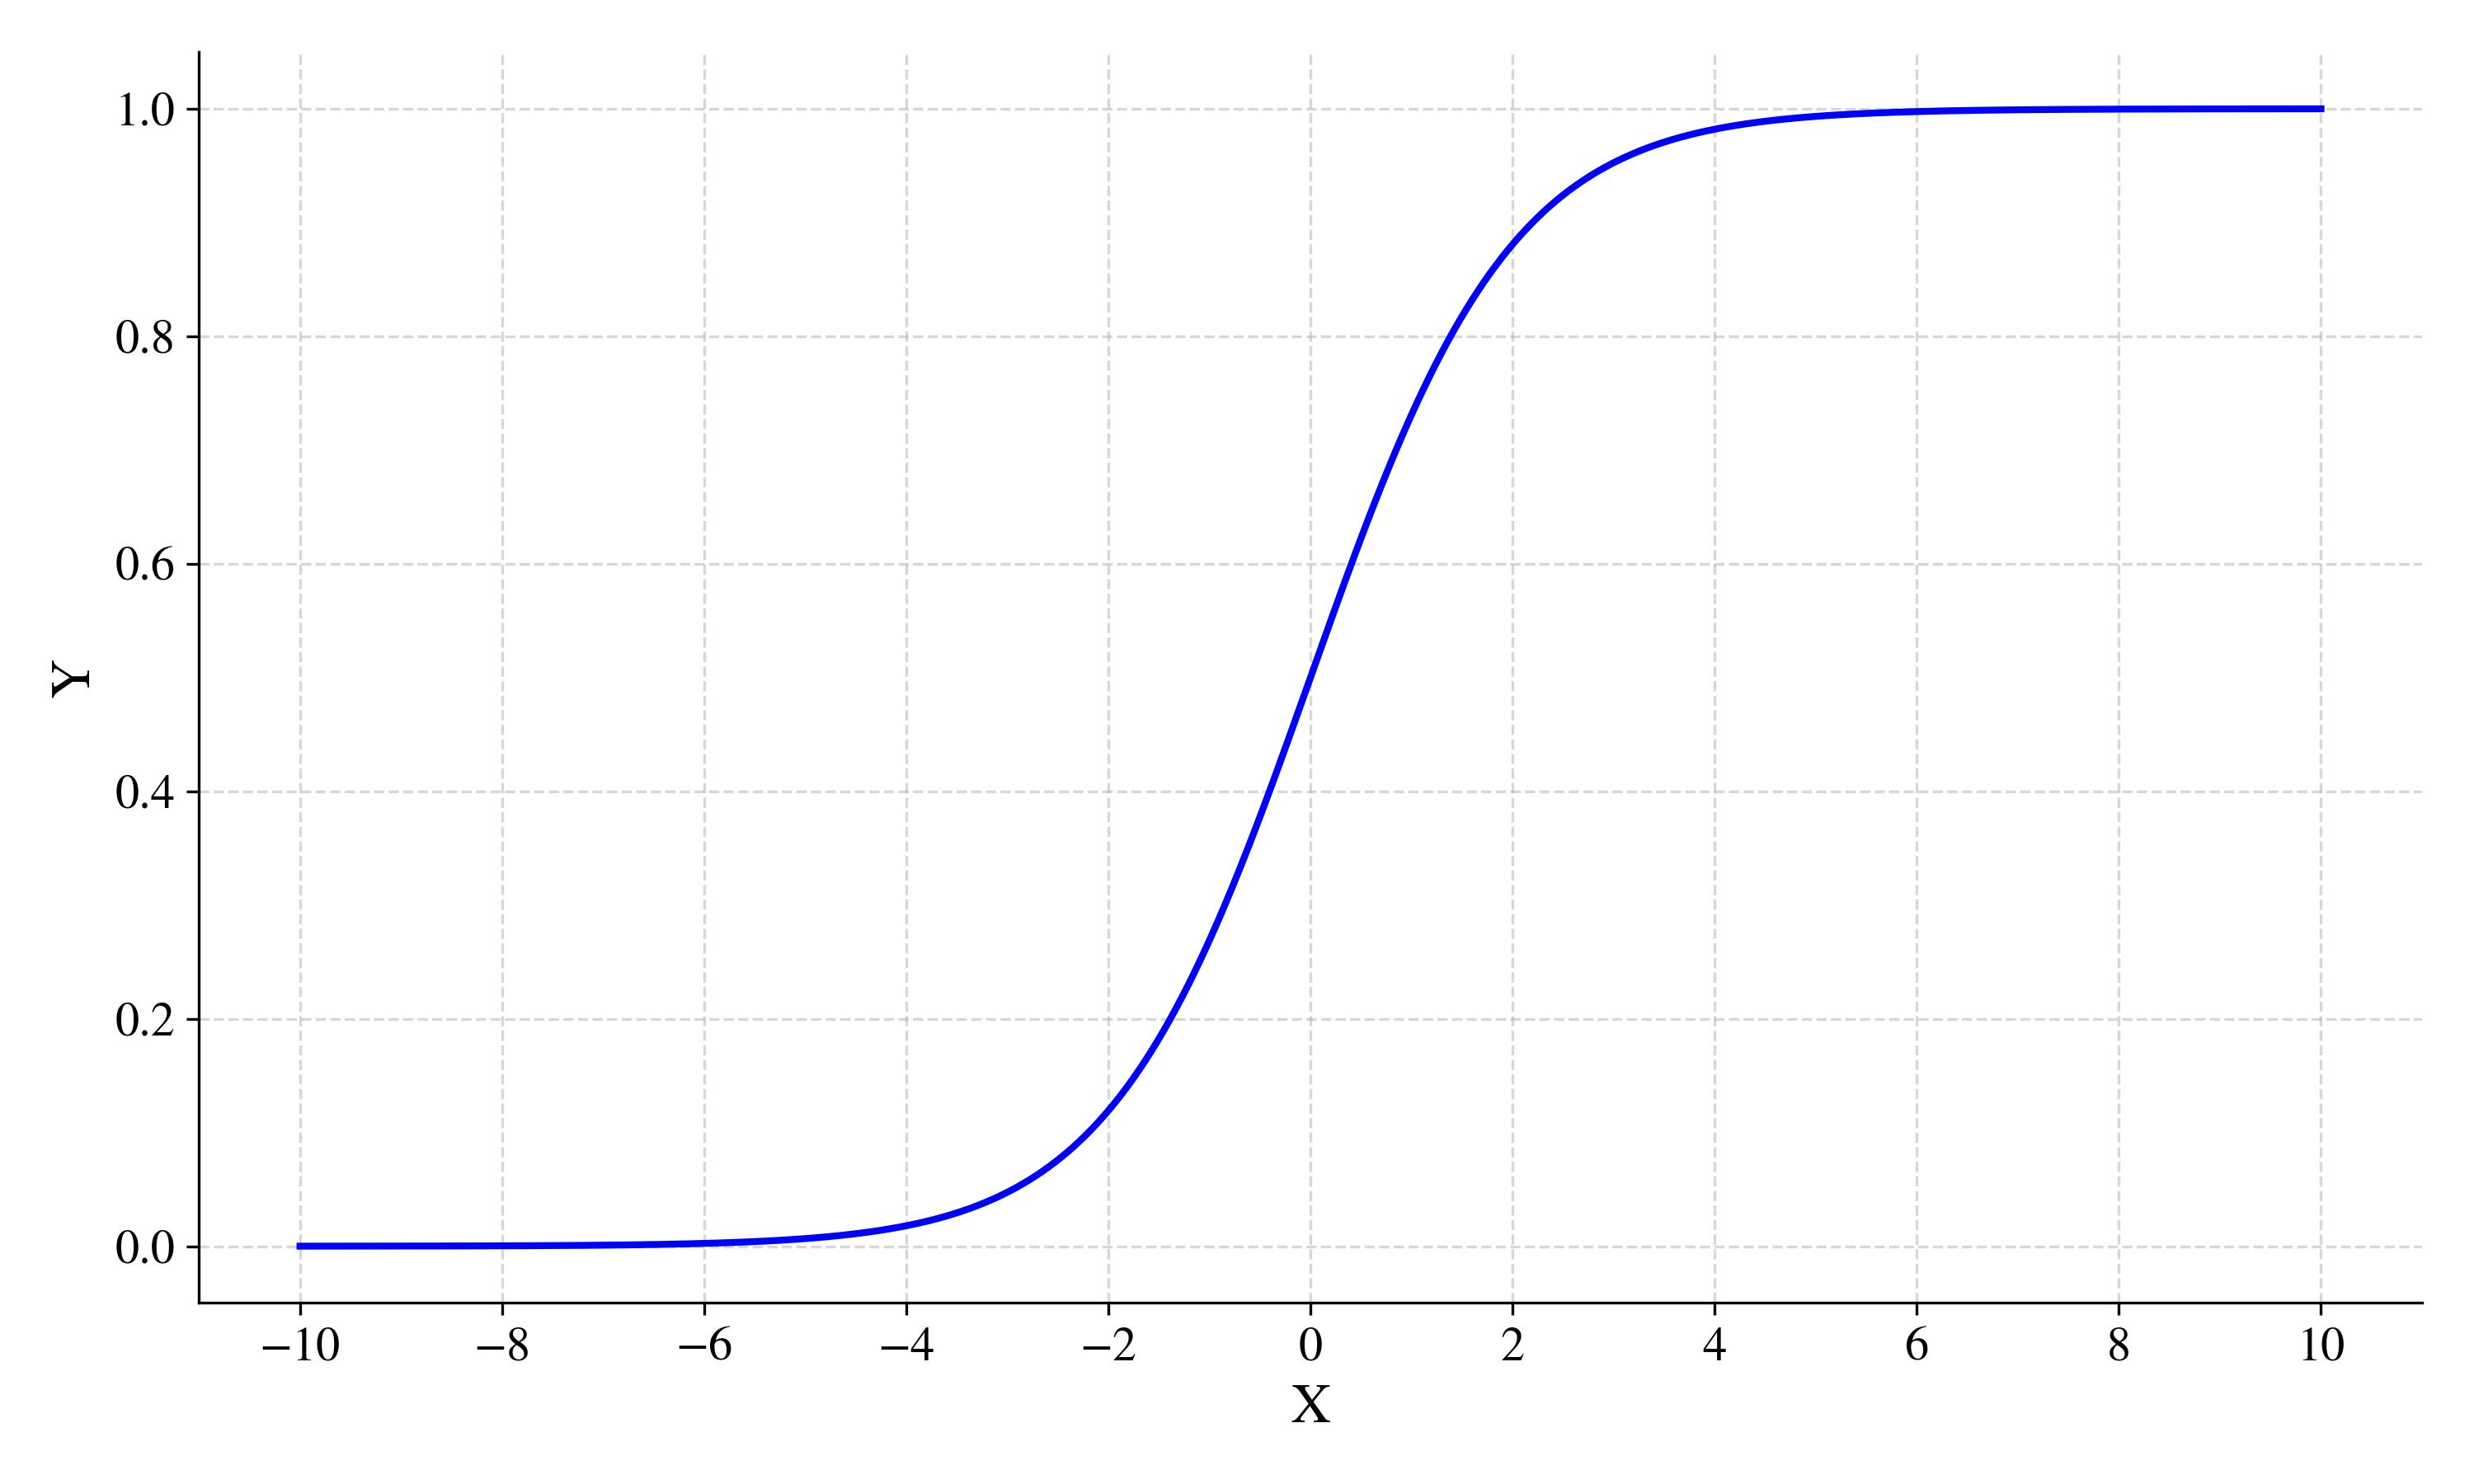
\includegraphics[width=130mm]{Figures/sigmoid.jpg}
    \centering{\begin{source}Author's simulation in Python\end{source}}\vspace{-1em}
\end{figure}

The linear form of the logistic regression with n features can be written as:

\begin{equation}\label{eq}
    \ln\left(\frac{P}{1-P}\right) = \beta_0  + \sum_{i=1}^{n} \beta_i X_i
\end{equation}

where $P$ is the probability of the occurred event, conditional on the set of given features. Let us denote $Y=1$ as an observed target instance where the event occurred (e.g., default), then:
\begin{equation}\label{eq}
    P = \operatorname{Pr}(Y=1 \mid X)
\end{equation}

Therefore, the term within the natural logarithm are the odds or more particularly, the ratio of the probability of the event with respect to the probability of non-event, both conditional on the same set of given features.
\begin{equation}\label{eq}
    \begin{aligned}
    \frac{P}{1-P}  {} & = \frac{\operatorname{Pr}(Y=1 \mid X_1,X_2,\ldots,X_n)}{1-\operatorname{Pr}(Y=1 \mid X_1,X_2,\ldots,X_n)} \\
    & = \frac{\operatorname{Pr}(Y=1 \mid X_1,X_2,\ldots,X_n)}{\operatorname{Pr}(Y=0 \mid X_1,X_2,\ldots,X_n)}
\end{aligned}
    \end{equation}

Referring to the previous equations, solving for $P$, henceforth we get a final equation for computing the probability of occurred event with usage of logistic regression:

\begin{equation}\label{eq}
P = \frac{1}{1+e^{-\left(\beta_0 + \displaystyle\sum_{i=1}^{n} \beta_i X_i\right)}}
\end{equation}

\subsection{Decision Tree}
\label{subsec:dt}

Decision tree (DT) is a rule--based algorithm which aims to partition the data into smaller and more homogeneous subsets. Such tree contains nodes, which are also visualized in \autoref{fig:dtnodes}, namely:
\begin{itemize}\setlength\itemsep{0em}
	\item Root node - the topmost node of the tree where the splitting begins.
	\item Internal node - the non--terminal nodes as a result of the split and can be further split into another subsets.
	\item Leaf node - the terminal nodes as a results of the split and cannot be further split into another subsets.
\end{itemize}
\begin{figure}[H]
    \centering
    \caption{Decision Tree's Nodes}\vspace{0.5em}
    \label{fig:dtnodes}\
    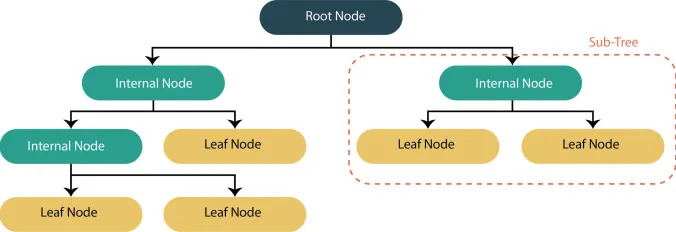
\includegraphics[width=130mm]{Figures/dtnodes.jpg}
    \centering{\begin{source}\citep{gauhar2020decision}\end{source}}\vspace{-1em}
\end{figure}

The splitting process is based on the homogeneity or so called purity of the node with respect to the target variable \citep{provost2013data}.
In other words, we want to have the node as pure as possible which means that the node should contain as high proportion of one class as possible.
In this case, the node should either contain high proportion of defaulters or non--defaulters, respectively.
Such splitting processs starts from the root node and continues until the leaf nodes are pure enough or until the stopping criteria are met.
The stopping criteria can be either a maximum depth of the tree, minimum number of observations within the node or minimum number of observations within the leaf node.
One way to measure impurity is using Entropy which ranges from 0 to 1 and is defined as:
\begin{equation}\label{eq}
    E = -\sum_{i=1}^{n} p_i \log_2 \left(p_i\right)
    \end{equation}
where $p_i$ is the probability of the occurrence of the event $i$, or in other words, it is a fraction of the observations belonging to the class $i$ within given node. In credit risk modelling terms, it is a proportion of defaulters within given node and $1-p_i$ is a proportion of non--defaulters within given sample.
The lower Entropy value, the purer the node is, i.e., the more homogeneous the subset is, where the frequency of one class is dominant to other class.
Therefore, the goal is to minimize the Entropy value since we want to have the purest nodes as possible, i.e., the nodes where is either a high proportion of defaulters or non--defaulters. 
However, the Entropy is not the only way to measure the impurity of the node. Another way is using Gini Impurity which ranges from 0 to 0.5 and is defined as:
\begin{equation}\label{eq}
    G = 1 - \sum_{i=1}^{n} p_{i}^{2}
\end{equation}
Both impurity measures are depicted in \autoref{fig:impurity} which we want to both of them minimize. Thus, we choose such feature and such rule which result in the lowest impurity measure. Such process is repeated until the stopping criteria are met or until the leaf nodes are pure enough.
\begin{figure}[H]
    \centering
    \caption{Gini Impurity vs. Entropy}\vspace{0.5em}
    \label{fig:impurity}\
    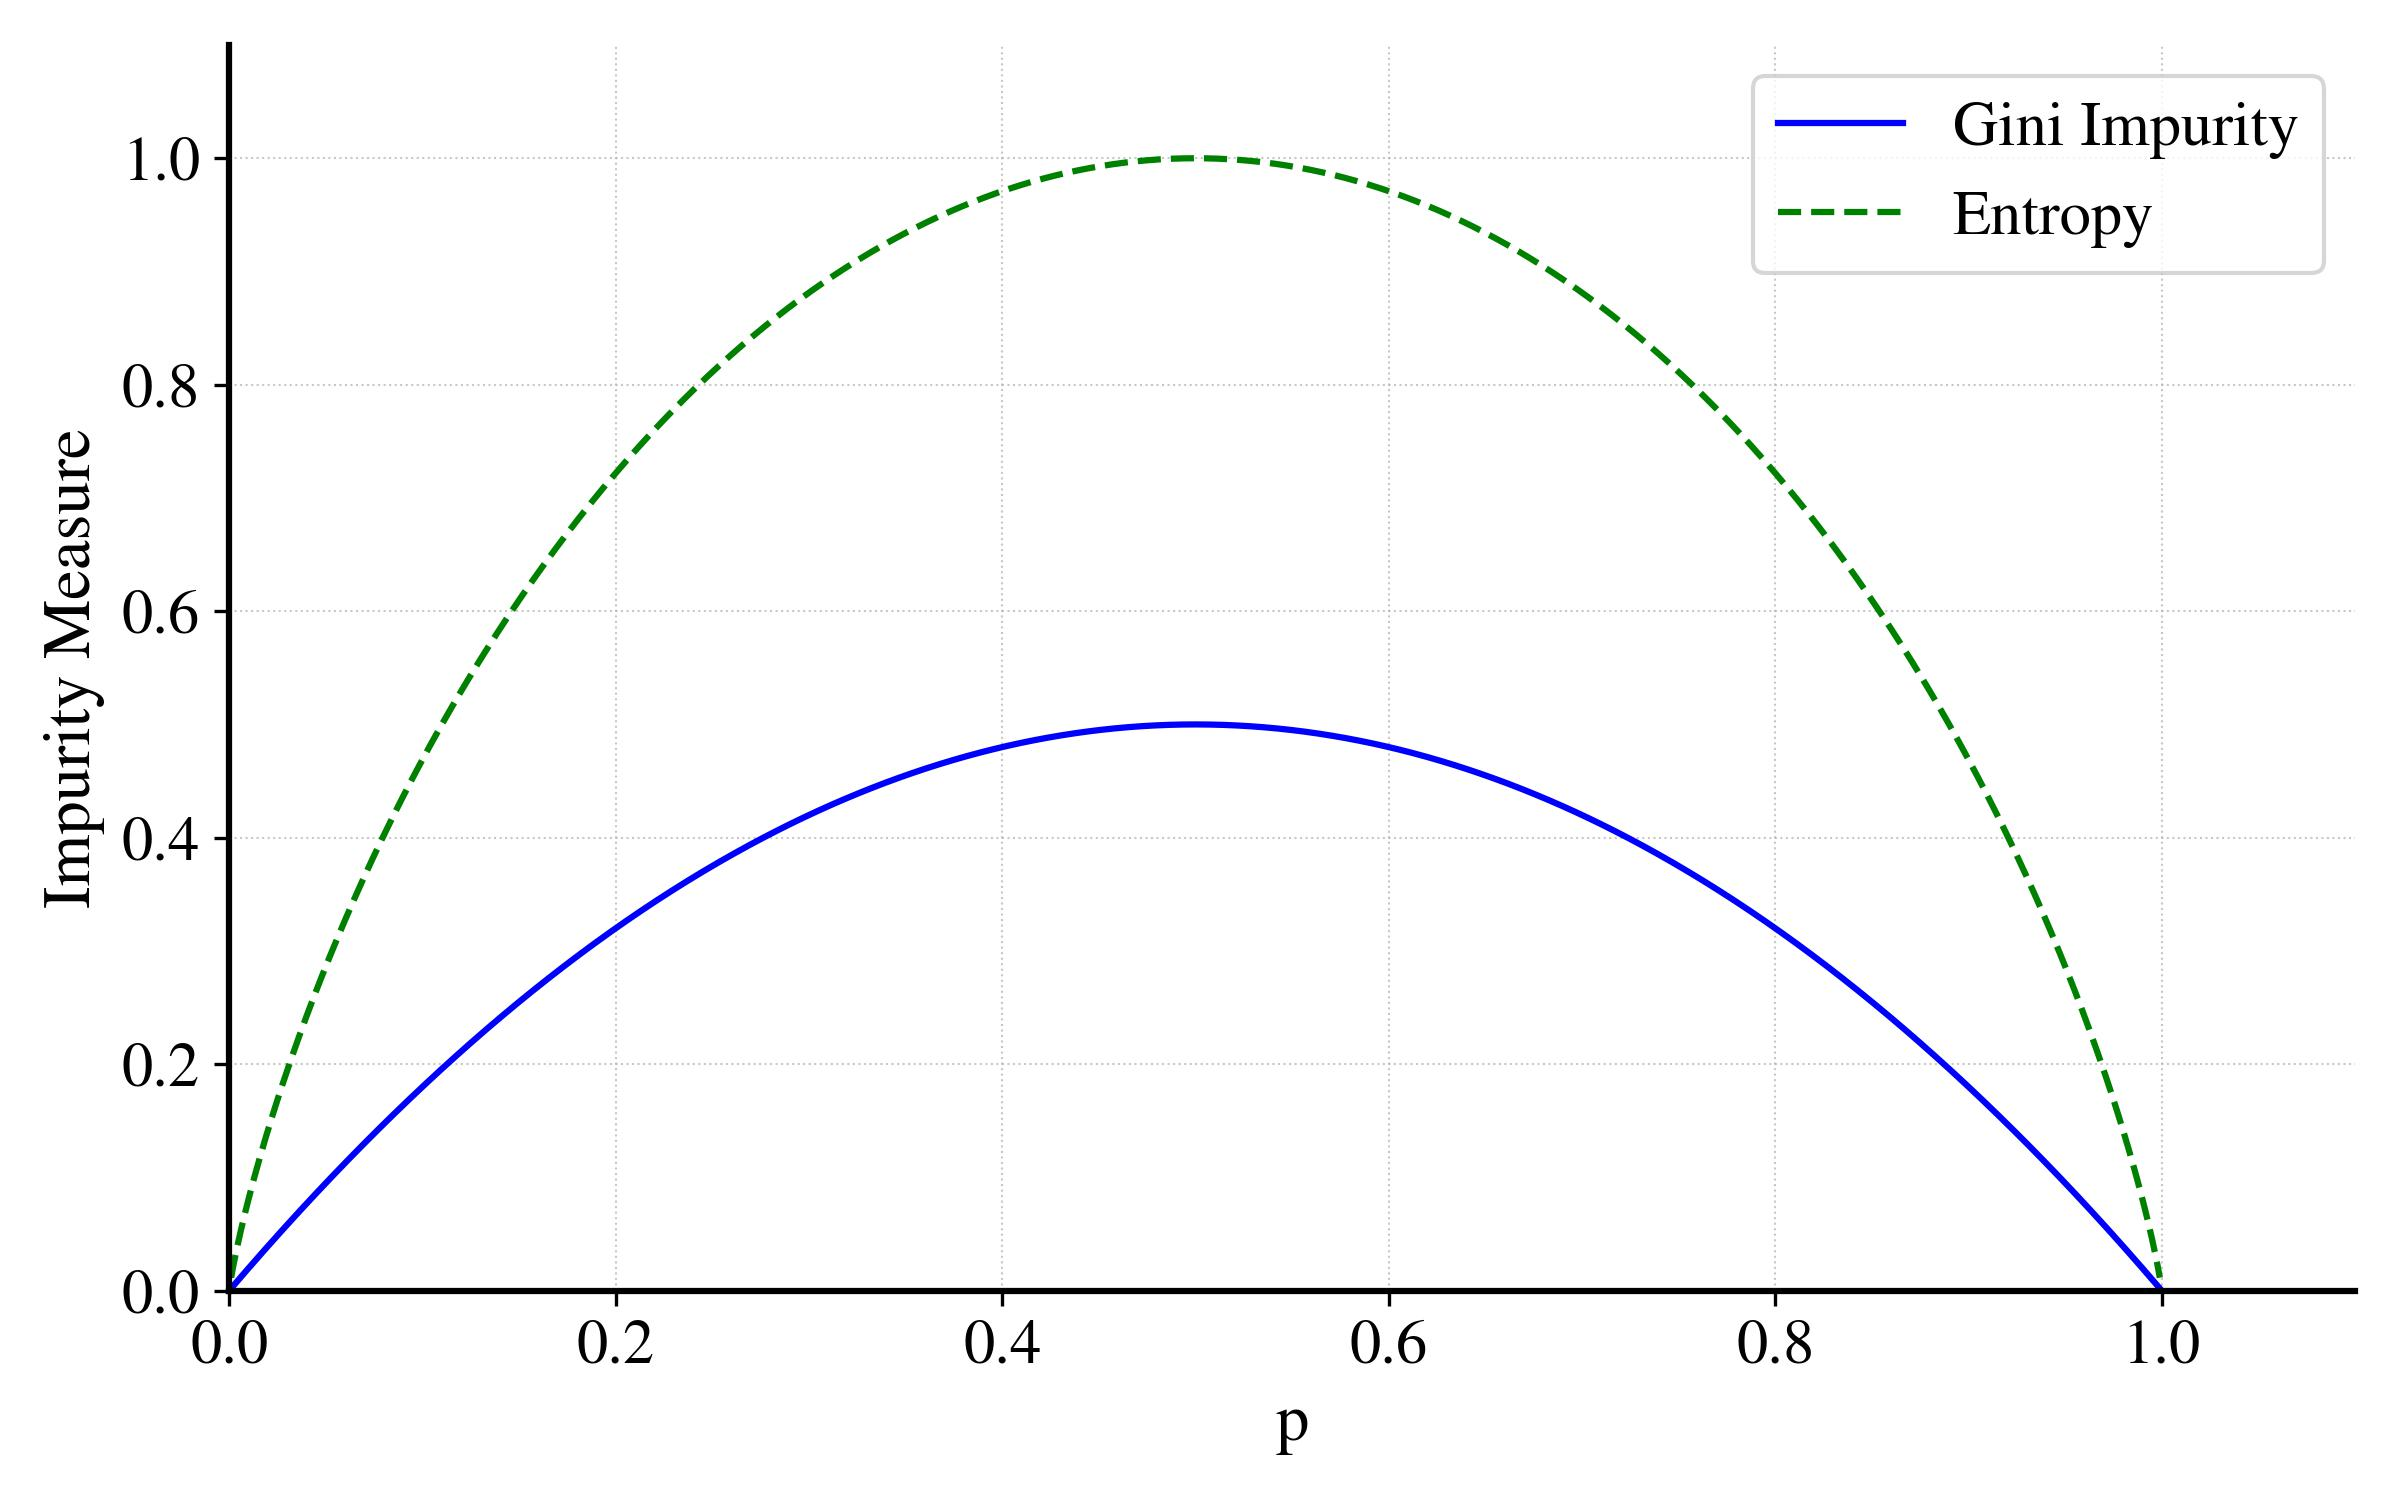
\includegraphics[width=130mm]{Figures/impurity.jpg}
    \centering{\begin{source}Author's simulation in Python\end{source}}\vspace{-1em}
\end{figure}

After the training, the DT predicts the target variable based on the rules which are stored in the tree.
The prediction process starts from the root node and continues until the leaf node is reached. Within the leaf node, the prediction can be either the most frequent class within the node or the probability of the occurrence of the event, i.e., the proportion of defaulters within given node.

\subsection{Naive Bayes}

Naive Bayes is a classification and probabilistic machine learning algorithm which is based on the Bayes theorem:

\begin{equation}\label{eq}
    \operatorname{Pr}\left(C=c \mid E \right) = \frac{\operatorname{Pr}\left(C=c\right) \times \operatorname{Pr}\left(E \mid C=c\right)}{\operatorname{Pr}\left(E\right)}
\end{equation}

where:
\begin{itemize}\setlength\itemsep{0em}
	\item $\operatorname{Pr}\left(C=c \mid E \right)$ is the posterior probability which is the probability that the target variable $C$ takes on the class of interest $c$ after taking the evidence $E$.
	\item $\operatorname{Pr}\left(C=c\right)$  is the prior probability of the class $c$ is the probability we would assign to the class $c$ before seeing any evidence $E$.
	\item $\operatorname{Pr}\left(E \mid C=c\right)$ is the probability of seeing the evidence $E$ conditional on the given class $c$.
	\item $\operatorname{Pr}\left(E\right)$ is the probability of the evidence $E$.
\end{itemize}

With regards to the binary classification, we can substitute $Y$ as a target variable instead $C$, and set of features $X$ which will refer to the set of evidence $E$., henceforth the probability of $Y$ using the Naive Bayes algorithm can be mathematically expressed as:

\begin{equation}\label{eq}
    \operatorname{Pr}\left(Y \mid X \right) = \frac{\operatorname{Pr}\left(Y\right) \times \operatorname{Pr}\left(X \mid Y \right)}{\operatorname{Pr}\left(X\right)}
\end{equation}

One of the assumptions of this algorithm is the conditional probabilistic independence among the features.
Since all the $X$ features' values combinations do not have to appear at all, we assume their independence \citep{cichosz2014data}.
Therefore, instead of computing the probability of all features together, conditional on the class event, for each feature $X$ we the conditional joint probability of $X$ given the class event. Hence:
\begin{equation}\label{eq}
    \operatorname{Pr}\left(X  \mid Y \right) = \prod_{i=1}^{n} \operatorname{Pr}\left(X_i \mid Y\right)
\end{equation}

Furthermore, the second adjustment is applied to the denominator of the Bayes theorem, i.e., $\operatorname{Pr}\left(X\right)$ - since such probability is constant over all the values of the class event, we can omit it from the equation. Therefore, the probability of the class event $Y$ can be expressed as:
\begin{equation}\label{eq}
    \operatorname{Pr}\left(Y \mid X \right) = \prod_{i=1}^{n} \operatorname{Pr}\left(X_i \mid Y\right) \times \operatorname{Pr}\left(Y\right)
\end{equation}

During the training process, the Naive Bayes algorithm computes $\operatorname{Pr}\left(Y\right)$ and $ \operatorname{Pr}\left(X \mid Y \right)$ for each class event $Y$ and each feature $X$.
In terms of default status, it calculates the proportion of defaulters  $\operatorname{Pr}\left(Y = 1\right)$ and non--defaulters $\operatorname{Pr}\left(Y=0\right)$ within given training sample as well as the proportion of defaulters and non--defaulters within given feature $X$.


When it comes to the predictions or classification of new instances, we use the trained Naive Bayes model, i.e., the computed probabilities $\operatorname{Pr}\left(Y\right)$ and $ \operatorname{Pr}\left(X \mid Y \right)$ for both default and non--default class.
Specifically, based on the new instance's features $X$, we determine the computed $\operatorname{Pr}\left(Y\right)$ and $ \operatorname{Pr}\left(X \mid Y \right)$ for both classes and aftewards, as a predicted class, we choose such class with the highest posterior probability. In general, the prediction while maximizing posterior probability is given as:
\begin{equation}\label{eq:nb-corrected}
    \operatorname{Pr}\left(Y \mid X \right) = \operatorname{argmax}_{y \in Y} \operatorname{Pr}\left(X \mid Y = y\right) \times \operatorname{Pr}(Y = y)
\end{equation}
Specifically, in terms of binary classification for prediction of given class, whether it is default or non--default, we can compute the probability of the default event ($1$) and non--default event ($0$) and choose the class with the higher probability.
\begin{equation}\label{eq}
    \operatorname{Pr}\left(Y \mid X \right)  = \max \left(\operatorname{Pr}\left(Y=1 \mid X\right), \operatorname{Pr}\left(Y=0 \mid X\right)\right)
\end{equation}
where:
\begin{equation}
    \operatorname{Pr}\left(Y=0 \mid X \right) = \operatorname{Pr}\left(Y=0\right) \times \prod_{i=1}^{n} \operatorname{Pr}\left(X_i \mid Y=0\right)
\end{equation}
respectively:
\begin{equation}
    \operatorname{Pr}\left(Y=1 \mid X \right) = \operatorname{Pr}\left(Y=1\right) \times \prod_{i=1}^{n} \operatorname{Pr}\left(X_i \mid Y=1\right)
\end{equation}
\subsection{K-Nearest Neighbors}

The goal of K-nearest Neighbors algorithm (also known as KNN) is to find $k$ instances that are most similar to particular instances y in the n-dimensional space, where n is the number of features.
The principle of this algorithm consists in the similarity between the instances as it assumes that the similar instances are close to each other.
Based on the predetermined $k$ neighbors, it will predict the class based on the k nearest instances.


There are several ways how to measure the distance. The most used one is the Euclidean distance. Geometrically, it is a straight line between the two points  and within two-dimensional space, it can be derived from the Pythagorean theorem, where the hypotenuse is the straight line measuring the distance. In the n-dimensional space, we take the sum the squared differences between the data points $x$ and $y$, underneath the square root in order to compute the total Euclidean distance.
\begin{equation}\label{eq}
d_{Euclidean}(x,y) = \sqrt{\sum\limits_{i=1}^{n} (x_i - y_i)^2}
\end{equation}

Other distance measure is the Manhattan distance measure, which is known as a city block distance, referring to the real-life problems, more particularly in order to reach particular destination, we have to take the path in between the blocks.
Mathematically, it is similar to the Euclidean distance, but instead of squared differences, it sums the absolute differences between the data points.
\begin{equation}\label{eq}
d_{Manhattan}(x,y) = \sqrt{\sum\limits_{i=1}^{n} |x_i - y_i|}
\end{equation}

The last measure is the Minkowski distance which is the generalized form Euclidean or Manhattan distance respectively.
It depends on p which represents the order of the norm. Hence, the Euclidean distance has the second order of the norm, whereas Manhattan distance has the first order of the norm.
\begin{equation}\label{eq}
d_{Minkowski}(x,y) = \sqrt[p]{\sum\limits_{i=1}^{n} |x_i - y_i|^p}
\end{equation}

Within the training process, KNN memorizes training instances and afterwards when it encounters a new instance, it tries to search for such training instance(s) which most strongly resembles the new instance \citep{witten2011data}.
Therefore, After the training process, when it comes to the prediction, the KNN compares the new instance to the training instances, calculates the distances between the the new input and the training instances, and predicts the class based on on the majority voting within the $k$ nearest neighbors, or predicts the probability scores as the fraction of positive instances within the $k$ nearest neighbors.


On the following \autoref{fig:knn-example}, let us consider 2--dimensional space and that $k$ is equal to 4, hence we are looking at four nearest neighbors for such new instance. Further, let us consider two classes - red squares and green triangles.
By looking at the four nearest neighbors, we can observe that three out of the nearest neighbors are the red triangles.
Therefore, when applying majority voting, KNN would predict such instance as a red triangle, or would predict a probability score of 0.75 for the red triangle.

\begin{figure}[H]
    \centering
    \caption{K-Nearest Neighbors with $k=4$}\vspace{0.5em}
    \label{fig:knn-example}\
    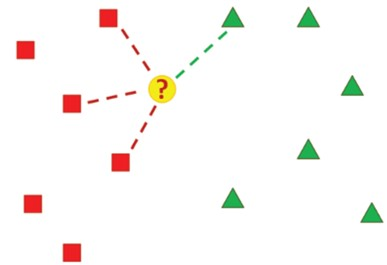
\includegraphics[width=80mm]{Figures/KNN_example.jpg}

    \centering{\begin{source}\citep{mucherino2009data}\end{source}}\vspace{-1em}
\end{figure}
\subsection{Random Forest}

Random forest is an ensemble algorithm which is a collection of decision trees where each tree is independently trained on on a bootstrap sample of the training data \citep{han2011data}, i.e., on a on a set which is randomly sampled from the training data with replacement which has the same size as the training data. In such way, each bootstrap sample is unique and can contain duplicates of the original data or does not have to contain all the original data.
Another aspect of randomness in such algorithm, particularly in the variability within trees, is the number of features considered for the split at each node.
Instead of considering all the features of the length $M$, it randomly selects a subset of features of the length $m$ (where $m<M$) and chooses the best split from the subset.
The training process of individual decision tree is the same as described in \autoref{subsec:dt}.

Within classifying new instances, the random forest algorithm predicts the class based on the majority voting of the individual decision trees or predicts a probability as an average of the probabilities of the individual decision trees \citep{randomforestmalley}, thus:
\begin{equation}
    \operatorname{Pr}\left(Y=1 \mid X \right) = \frac{1}{B} \sum_{b=1}^{B} \operatorname{Pr}\left(Y=1 \mid X, T_b \right)
\end{equation}
where $B$ is the number of trees and $T_b$ is the $b$-th tree.

\textbf{TBD}
\subsection{Gradient Boosting}

\textbf{TBD}
\subsection{Support Vector Machine}

Support Vector Machine (henceforth SVM) is machine learning algorithm which can handle both linear and non--linear classification problems and tries to transform original training data into a higher dimension, where the class points are linearly separable by a (linear) decision boundary, also known as hyperplane \citep{han2011data}.
In particular, SVM tries to maximize the margin which is the distance between the separating hyperplane and the support vectors, i.e., the training data points which are equally closest and parallel to such hyperplane\citep{tatsat2020machine}. The hyperplane can be expressed as follows, where $X$ are the features data, $W$ is the vector of the weights and $b$ is the intercept:
\begin{equation}
    W \times X + b = 0
\end{equation}
Moreover, the distance between the hyperplane and any training data point is expressed as $\frac{1}{\|W\|}$, where $\|W\|$ is Euclidean the norm of the weight vector $W$.
In order to maximize the margin, we therefore maximize $\frac{2}{\|W\|}$ as we want to maximize both sides of below and above the hyperplane.
When the data are not linearly separable, SVM transforms the original data points into a higher dimensional space using non--linear mapping functions, also known as kernels \citep{han2011data}.
In general, kernel function for the training tuples $(X_i,X_j)$ can be expressed as:
\begin{equation}
    K(X_i,X_j) = \phi(X_i) \cdot \phi(X_j)
\end{equation}
where $\phi$ mapping function for high--dimensional transformation of the feature space. The most common kernel functions are:
\begin{itemize}\setlength\itemsep{0em}
    \item $h$--degree polynomial kernel
\end{itemize}
\begin{equation}
    K\left(X_i,X_j\right) = (X_i \cdot X_k + 1)^{h}
\end{equation}
\begin{itemize}\setlength\itemsep{0em}
    \item Gaussian radial basis kernel
\end{itemize}
\begin{equation}
    K(X_i,X_j) = \exp\left(-\gamma |X_i-X_j\|^{2}\right)
\end{equation}
\begin{itemize}\setlength\itemsep{0em}
    \item Sigmoid kernel
\end{itemize}
\begin{equation}
    K(X_i,X_j) = \tanh(\kappa X_i \cdot X_j - \delta)
\end{equation}





\subsection{Neural Network}
Neural Network is a black--box machine learning algorithm which can handle very complex and non--linear relationship between. It contains several layers where each unit have a certain number of units. In general, we distinguish 3 type of layers:
\begin{itemize}\setlength\itemsep{0em}
    \item \textbf{Input layer} - The initial layer wghich contains $n$ units, where $n$ is the number of features within the dataset.
    \item \textbf{Output layer} - The final final layer which contains $m$ units, where $m$ is the number of classes within the target variable. Since we assume only binary classification algorithms, therefore the output layer contains only one unit.
    \item \textbf{Hiden layer} - The intermediate layer which is always between the two layers - either between the input and output layer or even between other hidden layers.
    \end{itemize}
The most common type of hidden layer is the fully connected layer where each unit is connected to each unit of the previous layer and to each unit in the next layer.
Thus, each unit receives the inputs from the previous layer, performs the computation and feed the output to the next layer - such process is called \textit{feed--forward}, thus feed--forward neural networks \citep{charu2018neural}.
Within the receiving the inputs, let us assume an integration function $g$ which performs a linear combination of the inputs $x$ and the weights $w$, and adds a bias term $b$.
Therefore, the ouput value $z$ of the single unit in hidden layer is calculated as:
\begin{equation}
    z = g\left(X,w\right)= b + \sum_{m=1}^{M} w_m x_m
\end{equation}
where $M$ indicates the number of units in the previous layer.
Before the output value $z$ is passed to the next layer, it is transformed by an activation function $f$ which is usually a non--linear function. The most common activation functions are:
\begin{itemize}\setlength\itemsep{0cm}
\item \textbf{ReLU} - Rectified Linear Unit (henceforth ReLU) is half--linear function which is rectified from the negative values to zero. The ReLU function is defined as:
\end{itemize}
\begin{equation}
    f(z) = \max(0,z)
\end{equation}
\begin{itemize}\setlength\itemsep{0cm}
    \item \textbf{Tanh} - Hyperbolic tangent (henceforth Tanh) is another widely used non--linear activation function which reminds of the sigmoid function. The Tanh function is limited to the range between -1 and 1, and is defined as:
    \end{itemize}
\begin{equation}
    f(z) = \frac{e^z - e^{-z}}{e^z + e^{-z}}
\end{equation}
\begin{itemize}\setlength\itemsep{0cm}
    \item \textbf{Sigmoid} - The logistic function was already described in \autoref{subsubsec:logisticregression}. Such function is usually used in the last hidden layer before the output layer as it maps the output to the range between 0 and 1, i.e., the predicted probability for binary classification. In terms of $z$, the sigmoid function is defined as:
    \end{itemize}
\begin{equation}
    f(z) = \frac{1}{1+e^{-z}}
\end{equation}
The training of neural network is an iterative process, where within each iteration (also called as epoch), the neural network is fed with the input, pass through the (hidden) layers to the output. The output is then compared with the actual value and the error is calculated.
Here comes another property of neural network which is the back--propagation, which updates all the weights and biases starting from the last layer by a small amount until the error is minimized as much as possible \citep{ayyadevara2018pro}.
The error is then backpropagated through the network and the weights are updated. The process is repeated until the error is minimized.

\section{Evaluation Metrics}

\textbf{TBD}

This section focuses on particular measures through which it is possible to determine a predictive power of model in terms of its performance.
The are many ways, how to evaluate the model's performance, therefore, only the most common ones and the most relevant are further described.
Note, since default prediction regards classification tasks, therefore regression's evaluation metrics are omitted.
If not stated otherwise, the higher metric measure, the better the model's performance is.
\subsection{Confusion Matrix and Derived Metrics}


Confusion matrix is a table which summarizes the classification model's performance with respect to the actual classes and predicted classes.
It is a square $n \times n$ matrix, where $n$ determines number of classes within the target variable.
Let us denote the confusion matrix as $C\left(f\right)$ for classification algorithm $f$. 
Its elements can be denoted as $c_{i,j}$ where $i$ and $j$ refer to the row and column indices, respectively, or more particularly, $i$ refers to the actual class and $j$ to the class predicted by the classifier $f$.
Each element of the confusion matrix refers to the number of instances corresponding to actual class $i$ and predicted class $j$ \citep{japkowicz2011evaluating}. For instance, the element $c_2,1$ would refer to the number of instances which have the actual class $2$ but have been classified as class $1$.
Mathematically, the confusion matrix can be written as following:

\begin{equation}\label{eq}
C = {c_{i,j} = \sum_{l=1}^{m}[(y_l=i) \land (f(x_l)=j)]}
\end{equation}

Or either in matrix form as:

\begin{equation}\label{eq}
    C_{i \times j} = \begin{bmatrix}
    c_{1,1} & c_{1,2} & \cdots & c_{1,j} \\
    c_{2,1} & c_{2,2} & \cdots & c_{2,j} \\
    \vdots & \vdots & \ddots & \vdots \\
    c_{i,1} & c_{i,2} & \cdots & c_{i,j} \\
    \end{bmatrix}
\end{equation}

From the given matrix, the diagonal elements represent the numbers of correctly classified instances, whereas the non-diagonal elements represent the numbers of misclassified instances.
Further, let us consider a binary classification - hence, the confusion matrix will have a form of $2\times 2$.

\begin{equation}
    C_{2 \times 2} = \begin{bmatrix}
    c_{1,1} & c_{1,2} \\
    c_{2,1} & c_{2,2} \\
    \end{bmatrix}
\end{equation}


We can this rewrite confusion matrix as:

\begin{equation}
    C_{2 \times 2} = \begin{bmatrix}
    TP & FN \\
    FP & TN \\
    \end{bmatrix}
\end{equation}

where:
\begin{itemize}\setlength\itemsep{0em}
    \item TP is the True Positive which refers to the number of instances which correspond to the actual class $True$ and indeed have been correctly classified as class $True$.
	\item $FP$ is the False Positive which refers to the number of instances which correspond to the actual class $True$, but have been incorrectly classified as class $False$. In the statistics and hypothesis--testing terms, it can be also called as Type 1 Error.
	\item $FN$ is the False Negative which refers to the number of instances which correspond to the actual class $False$, but have been incorrectly classified as class $True$. In the statistics and hypothesis--testing terms, it can be also called as Type 2 Error.
	\item $TN$ is the True Negative which refers to the number of instances which correspond to the actual class $False$ and indeed have been correctly classified as class $False$.
\end{itemize}

\subsubsection{Accuracy}
Such metric ranges from 0 to 1 and it describes in relatives terms how many instances the model has correctly predicted. Thus, the goal is to minimize the number of False Positives and False Negatives, or in credit risk modelling terms, number of defaulters which the model has classified as non--defaulters and number of non--defaulters which the model has classified as defaulters.
However, accuracy is inappropriate metric for evaluation when having imbalanced class, i.e., where the distribution of the target variable is skewed.
In such case, the model can achieve a relatively high accuracy even though it is not able to predict the minority class correctly \citep{brownlee2021failure}, thus it would lead to the misleading results.
This is the case of the credit risk modelling, when the loan portfolio oftenly have a lot of non--defaults and few defaults.
Therefore, it is deemed appropriate to consider other metrics when having imbalanced class.
\begin{equation}\label{eq}
    Accuracy = \frac{TP + FN}{TP + TN + FP + FN}
\end{equation}

\subsubsection{Recall}
Such metric is also known as True Positive Rate (TPR) or Sensitivity, which also ranges from 0 to 1, and it describes in relative terms how many actual \textit{True} instances the model has correctly predicted out of all the \textit{True} instances. Thus, the goal is to minimize the number of False Negatives, i.e., number of defaulters which the model has classified as non--defaulters.
A lower value of recall could therefore indicates that either the model is not able to predict correctly the $True$ classes resulting in low number of True Positives and/or high number of False Negatives.
Recall metris is useful when having imbalanced class and should be used instead of accuracy metric as it measures the model's ability to correctly identify instances of the minority class (i.e., defaults).
Mathematically based on the confusion matrix elements, it can be computed as:
\begin{equation}\label{eq}
    Recall = \frac{TP}{TP + FN}
\end{equation}

\subsubsection{Precision}
This metric describes in relative terms how many predicted \textit{True} instances are actually \textit{True}. Thus, the goal is to minimize the number of False Positives, i.e., number of non--defaulters which the model has classified as defaulters.
A lower value of precision could therefore indicates that either the model is not able to predict correctly the $True$ classes (low number of True Positives) or its prediction of $True$ classes is noisy (high number of False Positives).
Precision is another metric which should be used instead of accuracy when having imbalanced class as it tt measures the model's ability to correctly identify instances of the minority class while minimizing false positives (i.e., non--default instances which the model has classified as default).
Similarly, Precision also ranges from 0 to 1 and can be derived from the confusion matrix as follows:
\begin{equation}\label{eq}
    Precision = \frac{TP}{TP + FP}
\end{equation}
\subsubsection{F1 Score}
F1 score incorporates both Recall and Precision into a single value and takes on values between 0 and 1 as well.
Is it defined as a weighted harmonic mean of these two metrics \citep{brabec2020model} (where both Recall and Precision have uniform weights), and the goal is to minimize False Positives and False Negatives at the same time as within accuracy.
Nevertheless, F1 score is deemed as more appropriate metric when dealing with imbalanced class as it provides more balanced evaluation of model's performance in imbalanced datasets compared to accuracy.
\begin{equation}\label{eq}
    F1 = \frac{2 \times Precision \times Recall}{Precision + Recall} = \frac{2 \times TP}{2 \times TP + FP + FN}
\end{equation}

\subsubsection{Matthews Correlation Coefficient}
The drawback of Recall, Precision and F1 score is they are asymmetric measures, i.e., they do not take into account the True Negatives.
Therefore, such metrics' values will differ if we swap the positive and negative classes \citep{chicco2020advantages}, e.g., 1 would indicate non--default and vice versa.
In order to overcome such drawback, Matthews Correlation Coefficient can be used as it is symmetric and it takes into account all the four elements of the confusion matrix as well as it captures imbalanced class issue.
Methodologically, Matthews Correlation Coefficient is defined as a discretization of Pearson correlation for the case of binary variables \citep{boughorbel2017optimal}.
Pearson correlation coefficient is defined as:
\begin{equation}\label{eq}
    r(x,y) = \frac{\sum\limits_{i=1}^n (x_i - \bar{x})(y_i - \bar{y})}{\sqrt{\sum\limits_{i=1}^n (x_i - \bar{x})^2} \sqrt{\sum\limits_{i=1}^n (y_i - \bar{y})^2}}
\end{equation}
Thus, assuming that $x$ is the vector of True labels and $y$ is the vector of predictions, the Matthews Correlation Coefficient can be defined as:
\begin{equation}\label{eq}
    MCC = \frac{TP \times TN - FP \times FN}{\sqrt{(TP + FP) (TP + FN) (TN + FP) (TN + FN)}}
\end{equation}
Matthews correlation coefficient ranges from -1 to 1, where 1 indicates perfect model's predictions, -1 indicates that model misclassifies all the instances and 0 indicates that model's predictions are not better than random guessing.
\subsection{AUC}

In order to derive Area Under the Curve ($AUC$), first we need to define Receiver Operating Characteristics ($ROC$) curve.
ROC curve is two-dimensional visualization of the model performance as a probability curve in terms of True Positive Rate ($TPR$) and False Positive Rate ($FPR$) based on varying the given threshold.

Briefly, it can be construct as following: First, we need to sort the instances by the predicted probability and based on the given probability, we set a threshold - what will be above the threshold will be classified as $True$ instance and what is below the threshold will be classified as $False$ instance.
Based on these classified instances, the confusion matrix can be constructed and via which we can compute the $TPR$ and $FPR$ values.
Thus, if the probability is 1, the threshold will be 1 as well and hence:
\begin{itemize}\setlength\itemsep{0em}
    \item $TPR$ will be 0 because there is no probability which is higher than 1 and hence, everything will be classified as $False$ which will result into $TP$ of 0, and subsequently into $TPR$ of 0 as well.
	\item $FPR$ will be 0, too - since everything will be classified as $False$, therefore $FP$ will be 0 which implies $FPR$ to be 0, too.
\end{itemize}
On the other hand, if the probability is 0, the threshold will be 0 as well and hence:
\begin{itemize}\setlength\itemsep{0em}
    \item $TPR$ will be 1 because there is no probability which is lower than 0 and hence, everything will be classified as $True$ which will result into $FN$ of 0, and subsequently into $TPR$ of 1.
	\item $FPR$ will be 1, too - since everything will be classified as $True$, therefore $TN$ will be 0 which implies $FPR$ to be 1.
\end{itemize}

Thus, based on each threshold, the $TPR$ and $FPR$ will be to coordinates for single point within the graph and based on such points, we can construct the ROC curve.
Such visualization on the following \autoref{fig:roccurvetheory}.d
Note the diagonal line represents a random model which randomly and correctly predicts the $True$ and $False$ classes in such way, that $FPR$ and $TPR$ are the same.
Logically, a decent model should perform better than the random model, thus it the ROC curve should be above the diagonal line.
Intuitively, the best possible theoretical model would have $TPR$ of 1 and $FPR$ of 0, meaning that all the $True$ actual classes should be predicted as $True$ and all the $False$ actual classes should not be classified as $True$
 Within the ROC curve, the given curve reaches the left top corner which corresponds to the coordinates of $TPR$ and $FPR$.

 \begin{figure}[H]
    \centering
    \caption{ROC Curve}\vspace{0.5em}
    \label{fig:roccurvetheory}\
    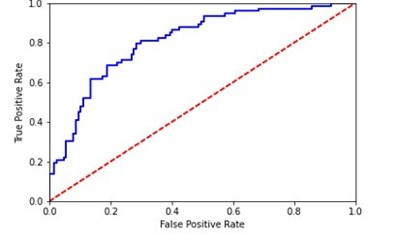
\includegraphics[width=100mm]{Figures/ROC_theory.jpg}

    \centering{\begin{source}Author's results in Python.\end{source}}\vspace{-1em}
\end{figure}

$AUC$ is basically the representation of ROC curve as a single number as it aggregates the performance on all possible thresholds.
$AUC$ can be interpreted as the probability that the randomly chosen actual $True$ instance is ranked higher than the randomly chosen actual $False$ instance.
Since ROC curve is a probability curve, thus it is considering distribution curve of $TP$ and distribution class of $TN$, separated by particular threshold – hence, $TP$ would have probability scores above the given thresholds, whereas $TN$ would have probability scores below the threshold.
If these curves do not overlap, meaning the model can perfectly distinguish between the $True$ and $False$ values, therefore the $AUC$ would be 1 and the ROC curve would reach the left top corner.
However, this idealistic situation does not occur in the practice at all, but rather the two distributions are overlapping since the misclassification of the classes takes the place.
The bigger overlap, the lower $AUC$ is.
If the distributions are completely overlapping, it implies the $AUC$ of 0.5, meaning that the model cannot distinguish between the $True$ and $False$ classes, which is the worst scenario.
On the other hand, if the distributions are totally opposite (meaning that the $TP$ instances would have probability scores below the given threshold, whereas the $TN$ instances would have probability scores above the given threshold), the $AUC$ would be 0 since the model is predicting the $True$ actual classes instead of $False$ and vice versa.

As the $AUC$ is an area present underneath the ROC curve, mathematically, it can be computed with the definite integral where $x$ is the given threshold:

\begin{equation}\label{eq}
    AUC = \int_{0}^{1} TPR \left(FPR^{-1}\left(x \right)\right) dx
\end{equation}

\subsection{Kolmogorov-Smirnov}

The Kolmogorov-Smirnov (KS) is non--parametric metric for assessing discriminant power of a model as it measures distance between the cumulative distribution functions (CDF) between two classes, and is quantified as a maximum vertical absolute difference between such two CDF's \citep{adeodato2016equivalence}.
In credit risk modelling terms, we can express KS as follows:
\begin{equation}\label{eq}
    \text{Kolmogorov Smirnov} = \max_{0 \le j \le 1} \left| F_D \left(j \right) - F_{ND} \left(j \right) \right|
\end{equation}
where $F_D$ and $F_{ND}$ are the cumulative distribution functions of default and non-default cases, respectively, and $j$ is the probability score threshold which ranges between 0 and 1.
\subsection{Somer's D}

The Somers' D is a metric which is part of the Kendall family of ranking measures. Particularly, assuming X-Y pairs, a Kendall's $\tau_{a}$ is defined as:
\begin{equation}\label{eq}
    \tau\left(X,Y\right) = \text{E} \left[ \text{sign}(X_i - X_j) \text{sign} (Y_i - Y_j) \right]
\end{equation}
Equivalently, Kendall's $\tau_{a}$ can be defined as the difference between the probability that the two X-Y pairs are \textit{concordant} and the probability that they are \textit{discordant}. X-Y pair is concordant if the larger of the $X$ values is paired with with larger of the $Y$ values, i.e, $X_i < X_j$ and $Y_i < Y_j$.
In contrast, X-Y pair is discordant if the larger of $X$ values is associated with smaller of $Y$ values or vice versa, i.e, $X_i < X_j$ and $Y_i > Y_j$, or $X_i > X_j$ and $Y_i < Y_j$ \citep{newson2002parameters}.
Therefore, Somers' D can be defined as the difference between the two conditional probabilities of concordance and discordance, given that the two $X$ values are unequal \citep{newson2014interpretation} as follows:
\begin{equation}
    D\left(Y \mid X\right) = \frac{\tau\left(X,Y\right)}{\tau\left(X,X\right)}
\end{equation}
In case of a binary classification, $X$ values would represent \textit{True} labels and $Y$ values would represent predicted probability scores as rank vectors. Such metric ranges from -1 to +1 (likewise as Matthews correlation coefficient +1). Thus, the higher value of Somers' D, the model's better ability to distinguish between borrowers who are likely to default and those who are not.

\subsection{Brier Score Loss}
Methodologically, Brier Score Loss is calculated in the same way as Mean Squared Error (MSE). However, Brier Score Loss is applied to the predicted probabilities (i.e., assumes that the target variable is dichotomous) \citep{comotto2022evaluation}, whereas MSE is rather used in regression tasks where is no assumption regarding the continuous target variable.
Henceforth, Brier Score Loss is defined as a mean squared error between the $True$ labels ($y$) and the predicted probabilities ($\hat{y}$) as follows:
\begin{equation}\label{eq}
    \text{Brier Score Loss} = \frac{1}{n} \sum_{i=1}^{n} (y_i - \hat{y}_i)^2
\end{equation}
Brier Score Loss ranges from 0 to 1, where the the ideal scenario would be Brier Score Loss of 0 - in such case, the model would be perfect predictive power.
\subsection{Jaccard Score}
Jaccard Score which is also known as Jaccard Index is a similarity metric as it measures similarity between the\textit{True} labels and predicted classes (0 or 1).
Let us denote $y$ as a vector of \textit{True} labels and $\hat{y}$ as a vector of predicted classes.
Hence, we can define Jaccard Score as the ratio of the size of intersection of $y$ and $\hat{y}$ to the size of union of $y$ and $\hat{y}$ \citep{leskovec2020mining}. Thus:
\begin{equation}\label{eq}
    \text{Jaccard Score} = \frac{|y \cap \hat{y} |}{|y \cup \hat{y} |}
\end{equation}
Likewise, Jaccard score ranges from 0 to 1 where the higher value indicates the higher similarity between the \textit{True} labels and predicted classes, hence the better model's performance.


\subsection{Log Loss}

Log loss, also know as logistic loss or cross--entropy loss, is a loss function metric which takes \textit{True} labels and predicted probabilities as an input and the minimize the difference between these two in a logarithmic function's form. Particularly, it indicates how close the predicted probabilities are to the corresponding $True$ labels. The more predicted probabilities diverges from the actual value, the more the log loss function penalizes the model's performance \citep{dembla2020intuition}.
\begin{equation}\label{eq}
    \text{Log Loss}  = -\frac{1}{N} \sum_{i=1}^{N} y_i \ln(p_i) + (1-y_i)\ln(1-p_i)
\end{equation}


Logically, the lower Log loss value, the better performance of the model is. As depicted in \autoref{fig:logloss}, we can observe the closer the predicted probability is closer to 1 with respect to the $True$ label being equal to 1, the more is the log loss function closer to 0 which is desired in terms of model's performance.
\begin{figure}[H]
    \centering
    \caption{Log Loss Function when $Y=1$}\vspace{0.5em}
    \label{fig:logloss}\
    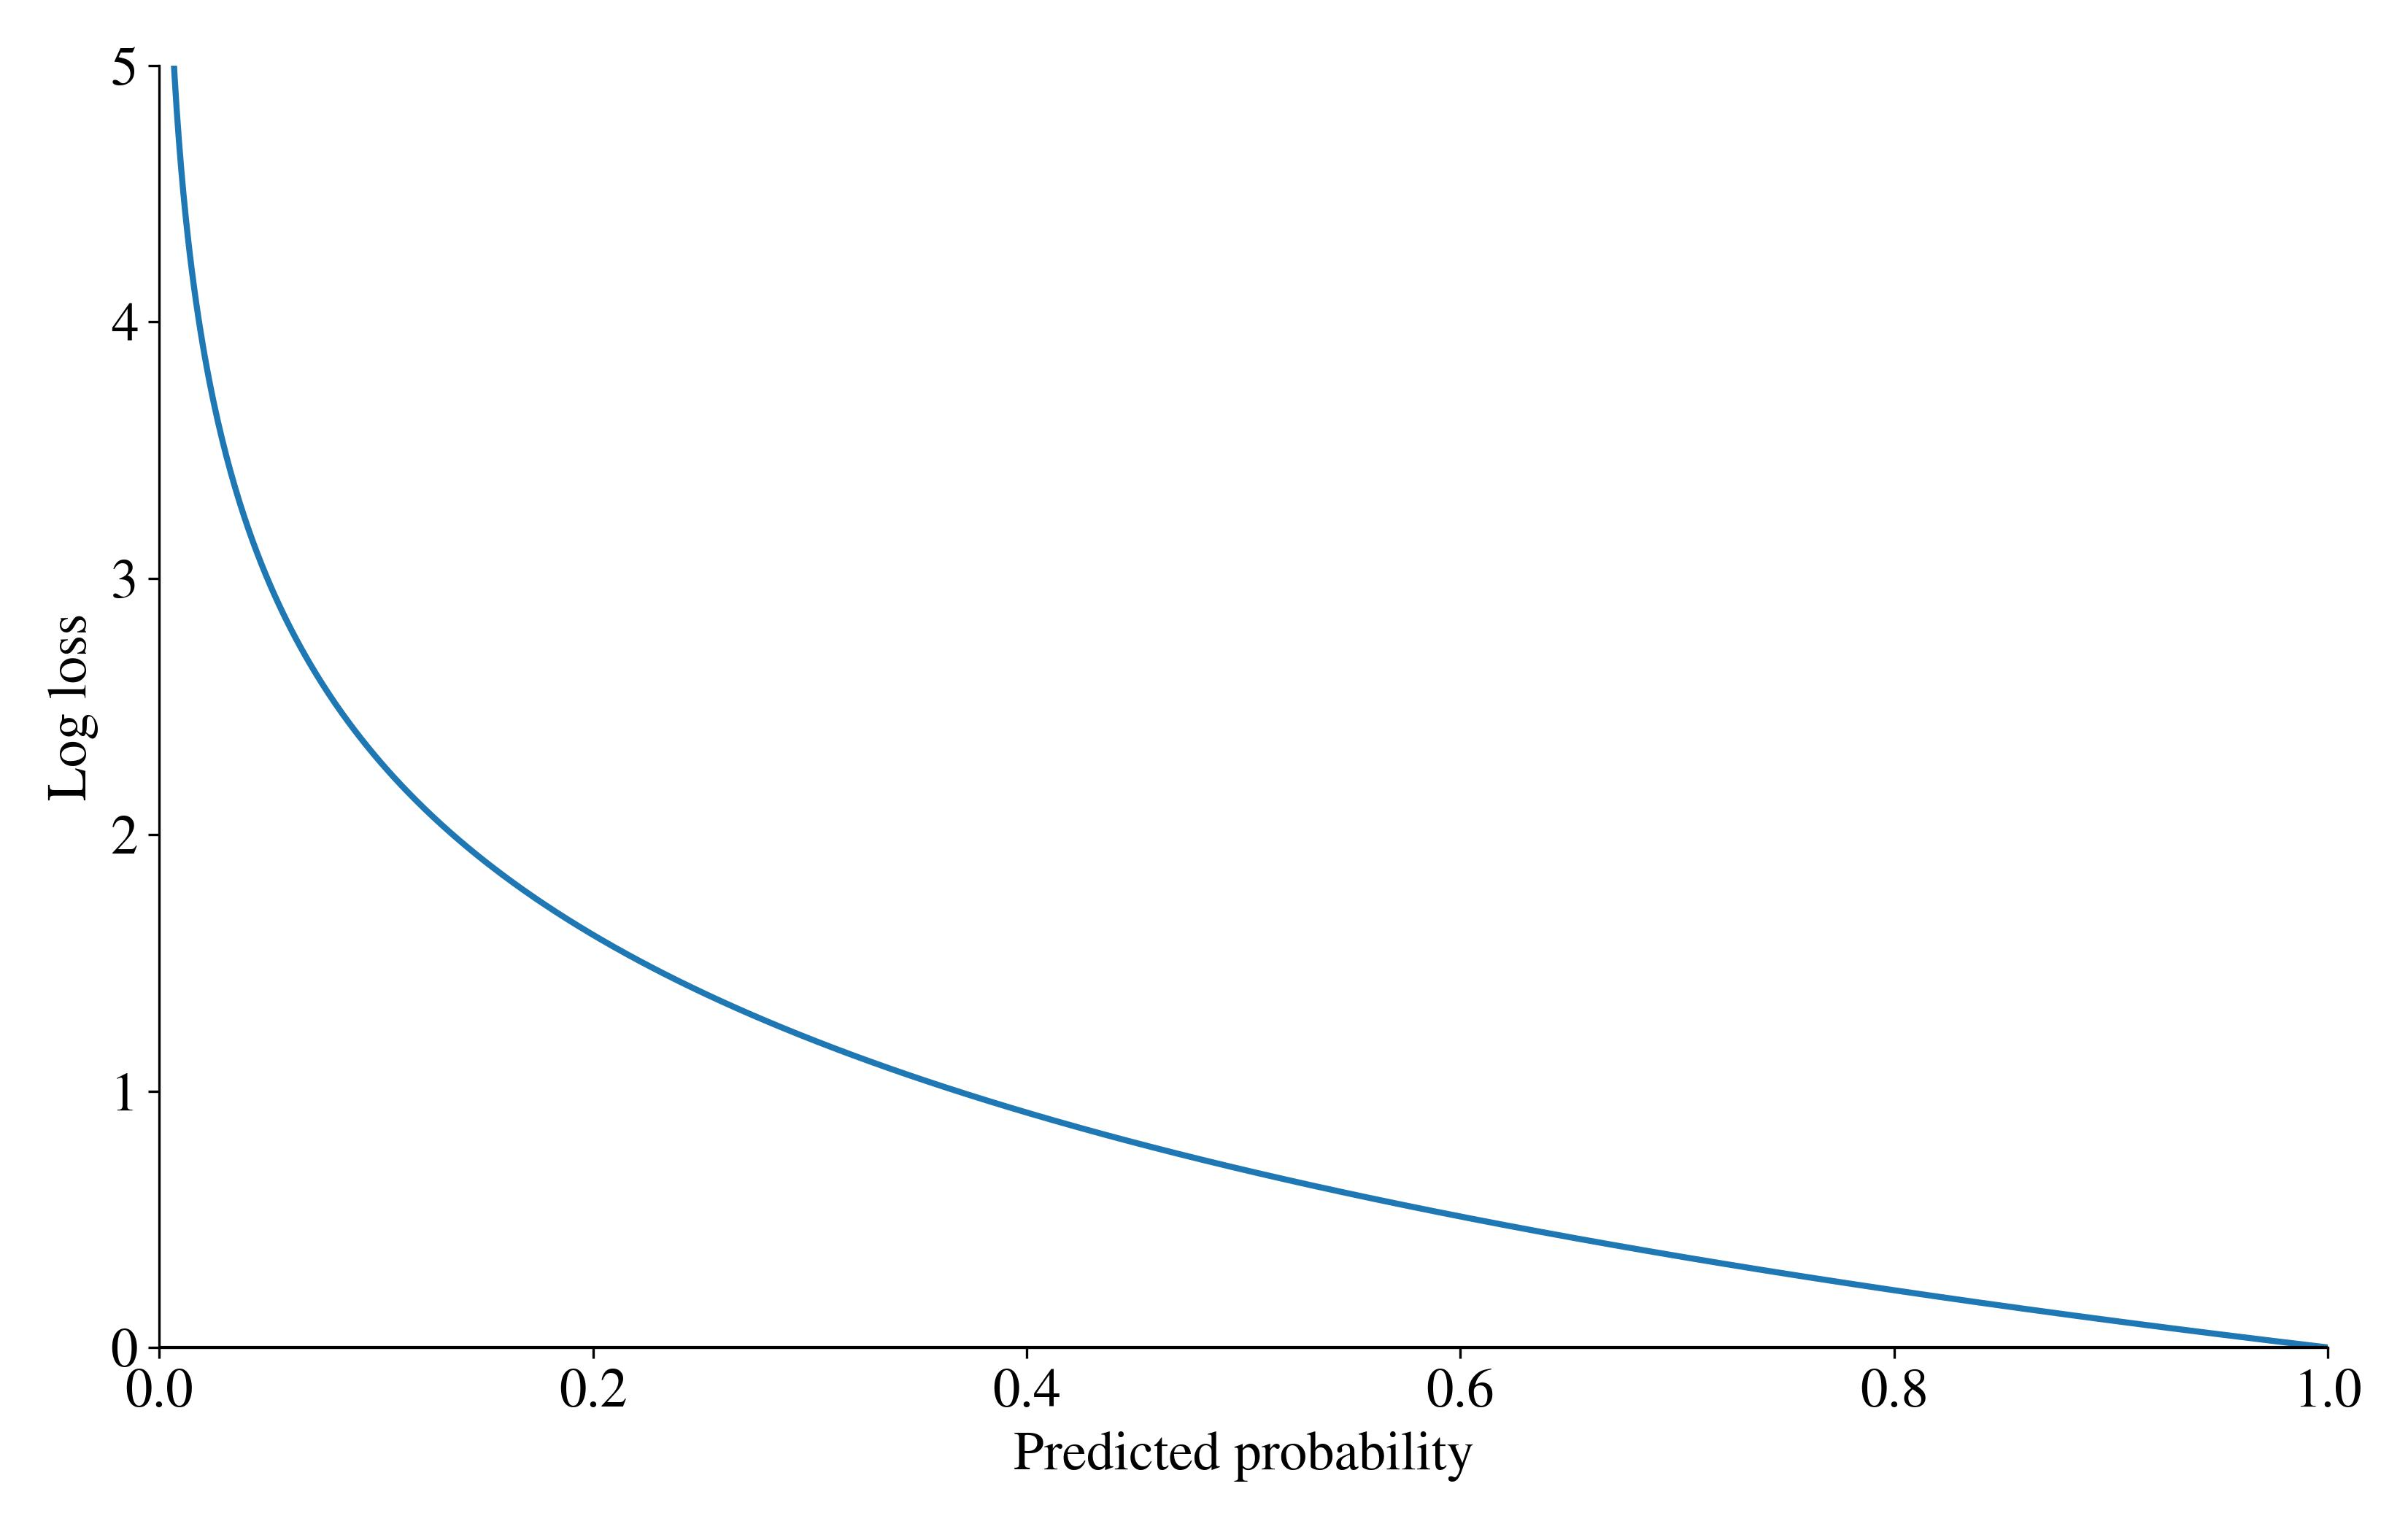
\includegraphics[width=130mm]{Figures/logloss.jpg}
    \centering{\begin{source}Author's simulation in Python\end{source}}\vspace{-1em}
\end{figure}
\chapter{Empirical Analysis - Machine Learning Implementation}
\label{chap:three}
This chapter focuses on the main part of this thesis, particularly on the practical example of machine learning implementation. The machine learning framework deployed in this thesis is shown in \autoref{fig:mlframe}.
\begin{itemize}\setlength\itemsep{0em}
\item \textbf{Data Exploration} - this part of the framework is focused on the exploration of the data in order to infer some insights about the data quality, distribution of the variables, statistical testing or association analysis.
\item \textbf{Data Split} - this part of the framework is focused on the splitting of the data which are used separaterly in diferrent tasks such as model training, model selection and model evaluation.
\item \textbf{Optimal Binning and WoE Encoding} - this part of the framework is focused on the optimal binning and the WoE encoding of the features as the main part of the feature preprocessing.
\item \textbf{Feature Selection} - this part of the framework is focused on the feature selection in order to reduce the dimensionality of the data and to improve the performance of the machine learning models - each input model estimator is tuned with Bayesian Optimization.
\item \textbf{Model Selection} - this part of the framework is focused on the model selection in order to find the best model based on the ranking - each input model is tuned with Bayesian Optimization on the subsets of selected features.
\item \textbf{Model Building (Evaluation)} - this part of the framework is focused on the recalibration of the final model by re-training it on the joined training and validation sets, which will be further evaluated.
\item \textbf{Model Evaluation} - this part of the framework is focused on the evaluation of the final model on the unseen data from test set.
\item \textbf{Model Building (Deployment)} - this part of the framework is focused on the final recalibration of the final model by re-training it on the joined training, validation and test sets, which will be further deployed into a production.
\item \textbf{Model Deployment} - this part of the framework is focused on the deployment of the final model into a production as a web application.
\end{itemize}

\begin{figure}[H]
\centering
\caption{Machine Learning Framework}\vspace{0.5em}
\label{fig:mlframe}
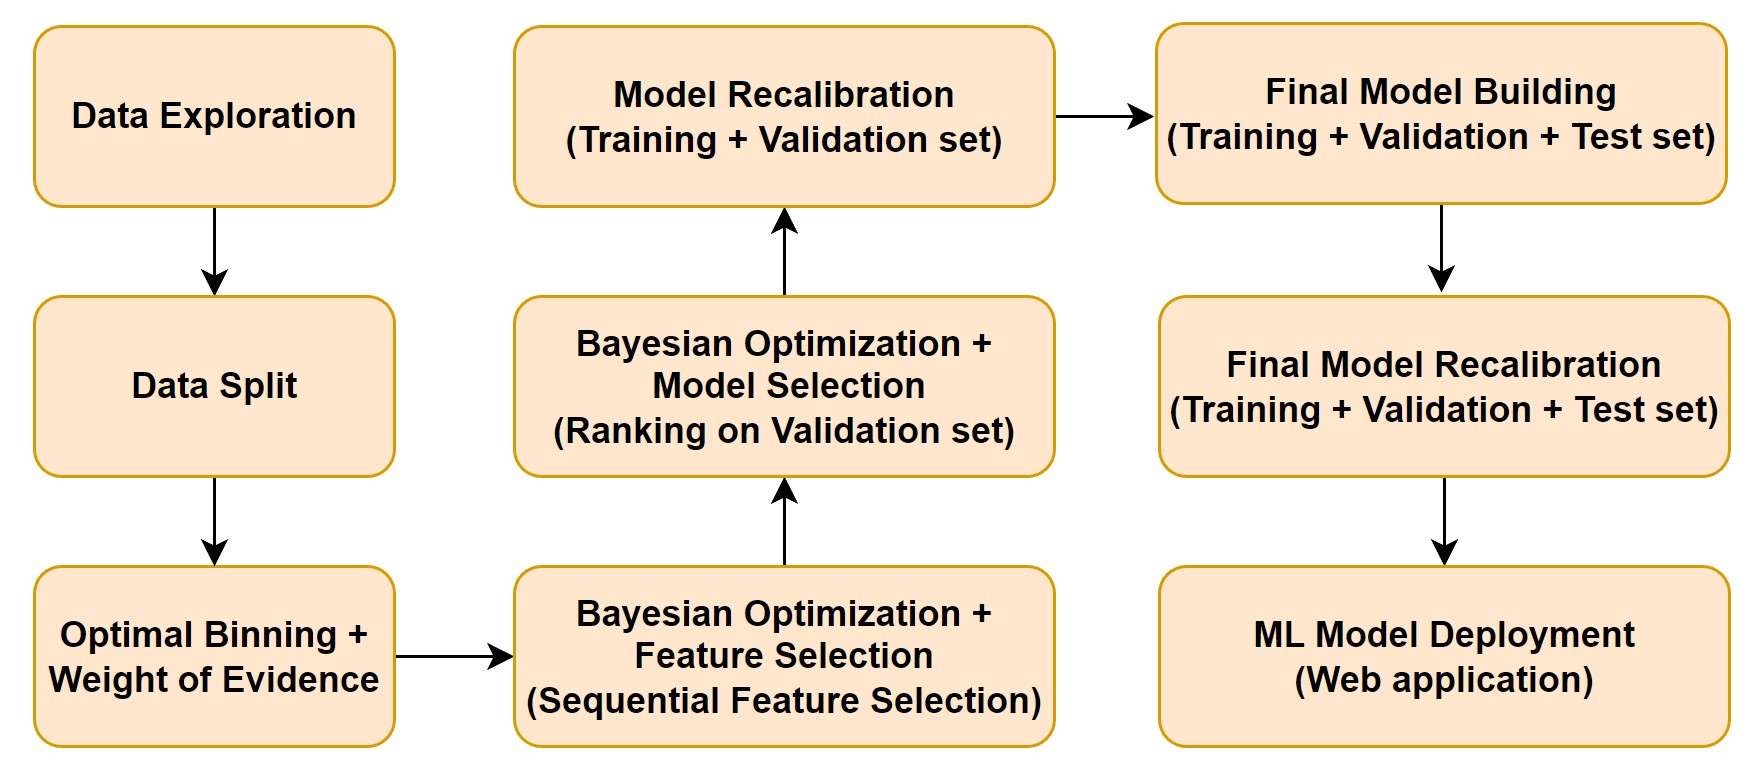
\includegraphics[width=120mm]{Figures/ml_framework.jpg}

\centering{\begin{source}Author's results\end{source}}\vspace{-1em}
\end{figure}

\section{Repository and Environment Structure}

The whole machine learning implmenetation as the scope of this thesis is done mainly using Python Programming Language and further with collaboration of Git and HTML.
The whole repository can be found in the separate appendix or is available on the GitHub repository \url{https://github.com/petr-ngn/FFU_VSE_Masters_Thesis_ML_Credit_Risk_Modelling}.
The repository structure is shown in \autoref{fig:repostructure}.
\begin{figure}[H]
\centering\caption{Repository Structure}
\label{fig:repostructure}

{\footnotesize
\begin{verbatim}

            |--- data
            |  |--- interim_dat.csv
            |  |--- preprocessed_data.csv
            |  |--- raw_data.csv
            |
            |--- flask_app
            |  |--- inputs
            |  |  |--- inputs_flask_app_dict.pkl
            |  |
            |  |--- templates
            |  |  |--- index.html
            |  |  |--- results.html
            |  |
            |  |--- static
            |  |
            |  |--- app.py
            |
            |--- models
            |  |--- feature_preprocessing
            |  |--- feature_selection
            |  |--- model_selection
            |  |--- objects_FINAL
            |
            |--- plots
            |--- Masters_Thesis.ipynb
            |--- README.md
            |--- requirements.yml
\end{verbatim}
}
\centering{\begin{source}Author's results at GitHub\end{source}}\vspace{0em}
\end{figure}


\begin{itemize}\setlength\itemsep{0em}
\item \texttt{data} - directory containing the raw data, partially preprocessed data (\texttt{interim}) and the final preprocessed data.
\item \texttt{flask\_app} - directory containing the Flask application which is used for the deployment of the model. Particularly, it contains the \texttt{app.py} file which is the main back-end file of the application, the \texttt{templates} and \texttt{static} subdirectories which contain the front-end HTML files for the application, and the \texttt{inputs} subdirectory which contains the input dictionary for the application (such as the trained model, threshold, final features etc.).
\item \texttt{models} - directory containing the the subdirectories of the trained and fitted objects for features preprocessing, feature selection and model selection, including the final objects used in deployment.
\item \texttt{plots} - directory containing the plots generated within the main Python notebook.
\item \texttt{Masters\_Thesis.ipynb} - main Python notebook containing the main part of the machine learning Implementation, such as exploratory analysis, data preprocessing, training and evaluation of the models.
\item \texttt{README.md} - README file containing the description of the repository.
\item \texttt{requirements.yml} - file containing the list of the required packages and their specific versions used in this project.
\end{itemize}

This particular solution is developed in Python version 3.10.9 and these are the main packages and modules used in this project:
\begin{itemize}\setlength\itemsep{0em}
\item \lstinline{NumPy}, \lstinline{Pandas} - for data manipulation and analysis.
\item \lstinline{Matplotlib}, \lstinline{Seaborn} - for data visualization.
\item \lstinline{Scipy} - for statistical analysis.
\item \lstinline{OptBinning} - for optimal binning of features with respect to the target.
\item \lstinline{ImbLearn} - for handling imbalanced data using oversampling.
\item {Scikit-learn} - for feature selection, model selection and model evaluation.
\item {Scikit-optimize} - for more advanced hyperparameter optimization.
\item {Flask} - for deployment of the model as web application.
\end{itemize}

To replicate this solution, one may download this repository as a zip file or either can clone this repository using Git to the local repository. Before running any files or scripts, it is important to set the environment for such project using the file \texttt{requirements.yml}. This can be done by running the following command in the Anaconda terminal which will create the new environment with the name \texttt{FFU\_VSE\_Masters\_Thesis} and install all the required packages:
\begin{figure}[H]
\centering\
{\footnotesize
\begin{verbatim}
>> conda env create -n FFU_VSE_Masters_Thesis -f requirements.yml    
\end{verbatim}
\vspace{-1em}
}
\end{figure}
Be aware of your current path directory in your terminal. In order to install the file \texttt{requirements.yml}, you need to define a path to the directory, where such file is located.
To achieve this, the user has to either change the path in the terminal using \texttt{cd} command, insert the path directory before the \texttt{requirements.yml} in terminal, or to copy the file \texttt{requirements.yml} to the current path directory. The following code shows the former approach:
\begin{figure}[H]
\centering\
{\footnotesize
\begin{verbatim}
>> cd C:\Users\ngnpe\FFU_VSE_Masters_Thesis_ML_Credit_Risk_Modelling
>> conda env create -n FFU_VSE_Masters_Thesis -f requirements.yml   
\end{verbatim}
\vspace{-1em}
}
\end{figure}


To preserve the reproducibility of this solution and conistency of the results, the random seed is instantiated to \texttt{42}, so for instance data split, model optimization or training would be deterministic and not totally random everytime when replicating the solution.

Some \lstinline{Scikit-learn} or \lstinline{Scikit-optimize} objects have optional argument \texttt{n\_jobs} which utilizes the number of CPU cores used during the parallelizing computation. Such argument was set to \texttt{-1}, hence all the processors are used in order to  speed up the training or optimization process.


\section{Data Exploration}
This section is focused on exploration of the analyzed loan dataset, particularly on dataset description, distribution analysis and association analysis, in order to infer potential valuable insights and hypotheses which can be used in the preprocessing or modelling part.

\subsection{Dataset Description}
The analyzed dataset pertains to the HMEQ dataset which contains loan application information and default status of 5,960 US home equity loans. Such dataset was acquired from Credit Risk Analytics platform. Since this dataset regards the loan application scoring data, using macroeconomic or other external data is omitted due to the dataset characteristics as well as modelling with behavioral scoring.
Thus our goal is to predict whether the loan applicant will or would default based on provided information from the loan application.

As can be seen in \autoref{tab:dataset}, the dataset contains 13 columns, 12 features and 1 target variable \texttt{BAD} indicating whether the loan was in default (\texttt{1}) or not (\texttt{0}). 
Amongst the 12 features, there are 10 numeric features and 2 categorical features, namely \texttt{REASON} which contains 2 categories - Debt consolidation (\texttt{DebtCon}) and Home improvement (\texttt{HomeImp}), and \texttt{JOB} which fontains following categories - Administration (\texttt{Office}), Sales, Manager (\texttt{Mgr}), Professional Executive (\texttt{ProfExe}), Self-employed (\texttt{Self}), and Other.


\begin{table}[H]
\small
\setlength{\tabcolsep}{8pt}
\renewcommand{\arraystretch}{1.3}
\begin{center}
\caption[Dataset columns]{Dataset columns}\label{tab:dataset}
\begin{tabular}{@{} l p{8cm} l @{}}
\toprule
\textbf{Columns} & \textbf{Description} & \textbf{Data type}\\
\midrule
\hline
BAD & Default status & Boolean \\

LOAN & Requested loan amount & numeric \\

MORTDUE & Loan amount due on existing mortgage & numeric \\

VALUE & Value of current underlying collateral property & numeric \\

REASON & Reason of loan application & categorical \\
JOB & Job occupancy category & categorical \\

YOJ & Years of employment at present job & numeric \\

DEROG & Number of derogatory public reports & numeric \\

DELINQ & Number of delinquent credit lines & numeric \\

CLAGE & Age of the oldest credit line in months & numeric \\

NINQ & Number of recent credit inquiries & numeric \\

CLNO & Number of credit lines & numeric \\

DEBTINC & Debt-to-income ratio & numeric \\
\hline
\bottomrule
\end{tabular}
\end{center}
\begin{center} % Center the source
\source{\url{http://www.creditriskanalytics.net/datasets-private2.html}}
\end{center}
\end{table}

After the initial data inspection, data does not contain any duplicates but does contain missing values, which are summarized in \autoref{tab:natable}.
Most of the missing values contains the feature \texttt{DEBTINC} with 1,267 missing observations, whereas columns indicating default status (\texttt{BAD}) or requested loan amount (\texttt{LOAN}) do not contain any missing values, which is expected as the bank should have the available information about their loans whether they have defaulted or not, and since this dataset pertains to the application scoring, when applying for a loan, an applicant should always fill out the requested loan amount.

\begin{table}[H]
\small
\setlength{\tabcolsep}{8pt}
\renewcommand{\arraystretch}{1.3}
\centering
\caption[Missing Values Summary]{Missing Values Summary}\label{tab:natable}
\begin{tabular}{l r r}
\toprule
\textbf{Columns} & \textbf{\# NA's} & \textbf{\% NA's}\\
\midrule
\hline
BAD & 0 & 0.00 \% \\
LOAN & 0 & 0.00 \% \\
MORTDUE & 518 & 8.69 \% \\
VALUE & 112 & 1.88 \% \\
REASON & 252 & 4.23 \% \\
JOB & 279 & 4.68 \% \\
YOJ & 515 & 8.64 \% \\
DEROG & 708 & 11.88 \% \\
DELINQ & 580 & 9.73 \% \\
CLAGE & 308 & 5.17 \% \\
NINQ & 510 & 8.56 \% \\
CLNO & 222 & 3.72 \% \\
DEBTINC & 1267 & 21.26 \% \\
\hline
\bottomrule
\end{tabular}
\vspace{0.35em}

\centering{\begin{source}Author's results in Python\end{source}}\vspace{-1em}
\end{table}


\subsection{Distribution Analysis}
In this subsection, we inspect the distribution of our variables, including the target variable and the features.
Such distribution inspection may help us to identify potential outliers, missing values, and other potential issues with the dataset.

\subsubsection{Default Distribution}

Regarding the the target variable distribution, from the \autoref{fig:defaultdist} we can observe that the default status distribution is heavily imbalanced, as most of the loans have not defaulted yet.
Particularly, 80.05\% of the observations have been labelled as non-default (4,771 observations) and 19.95\% observations labelled as default (1,189 observations).
This may cause problems in the modelling part, as the model may be biased towards the majority class, i.e., the non-default class. Such imbalanced class issue will be further treated in \autoref{subsec:data-split-ADASYN}.

\begin{figure}[H]
\centering
\caption{Default status distribution}
\label{fig:defaultdist}
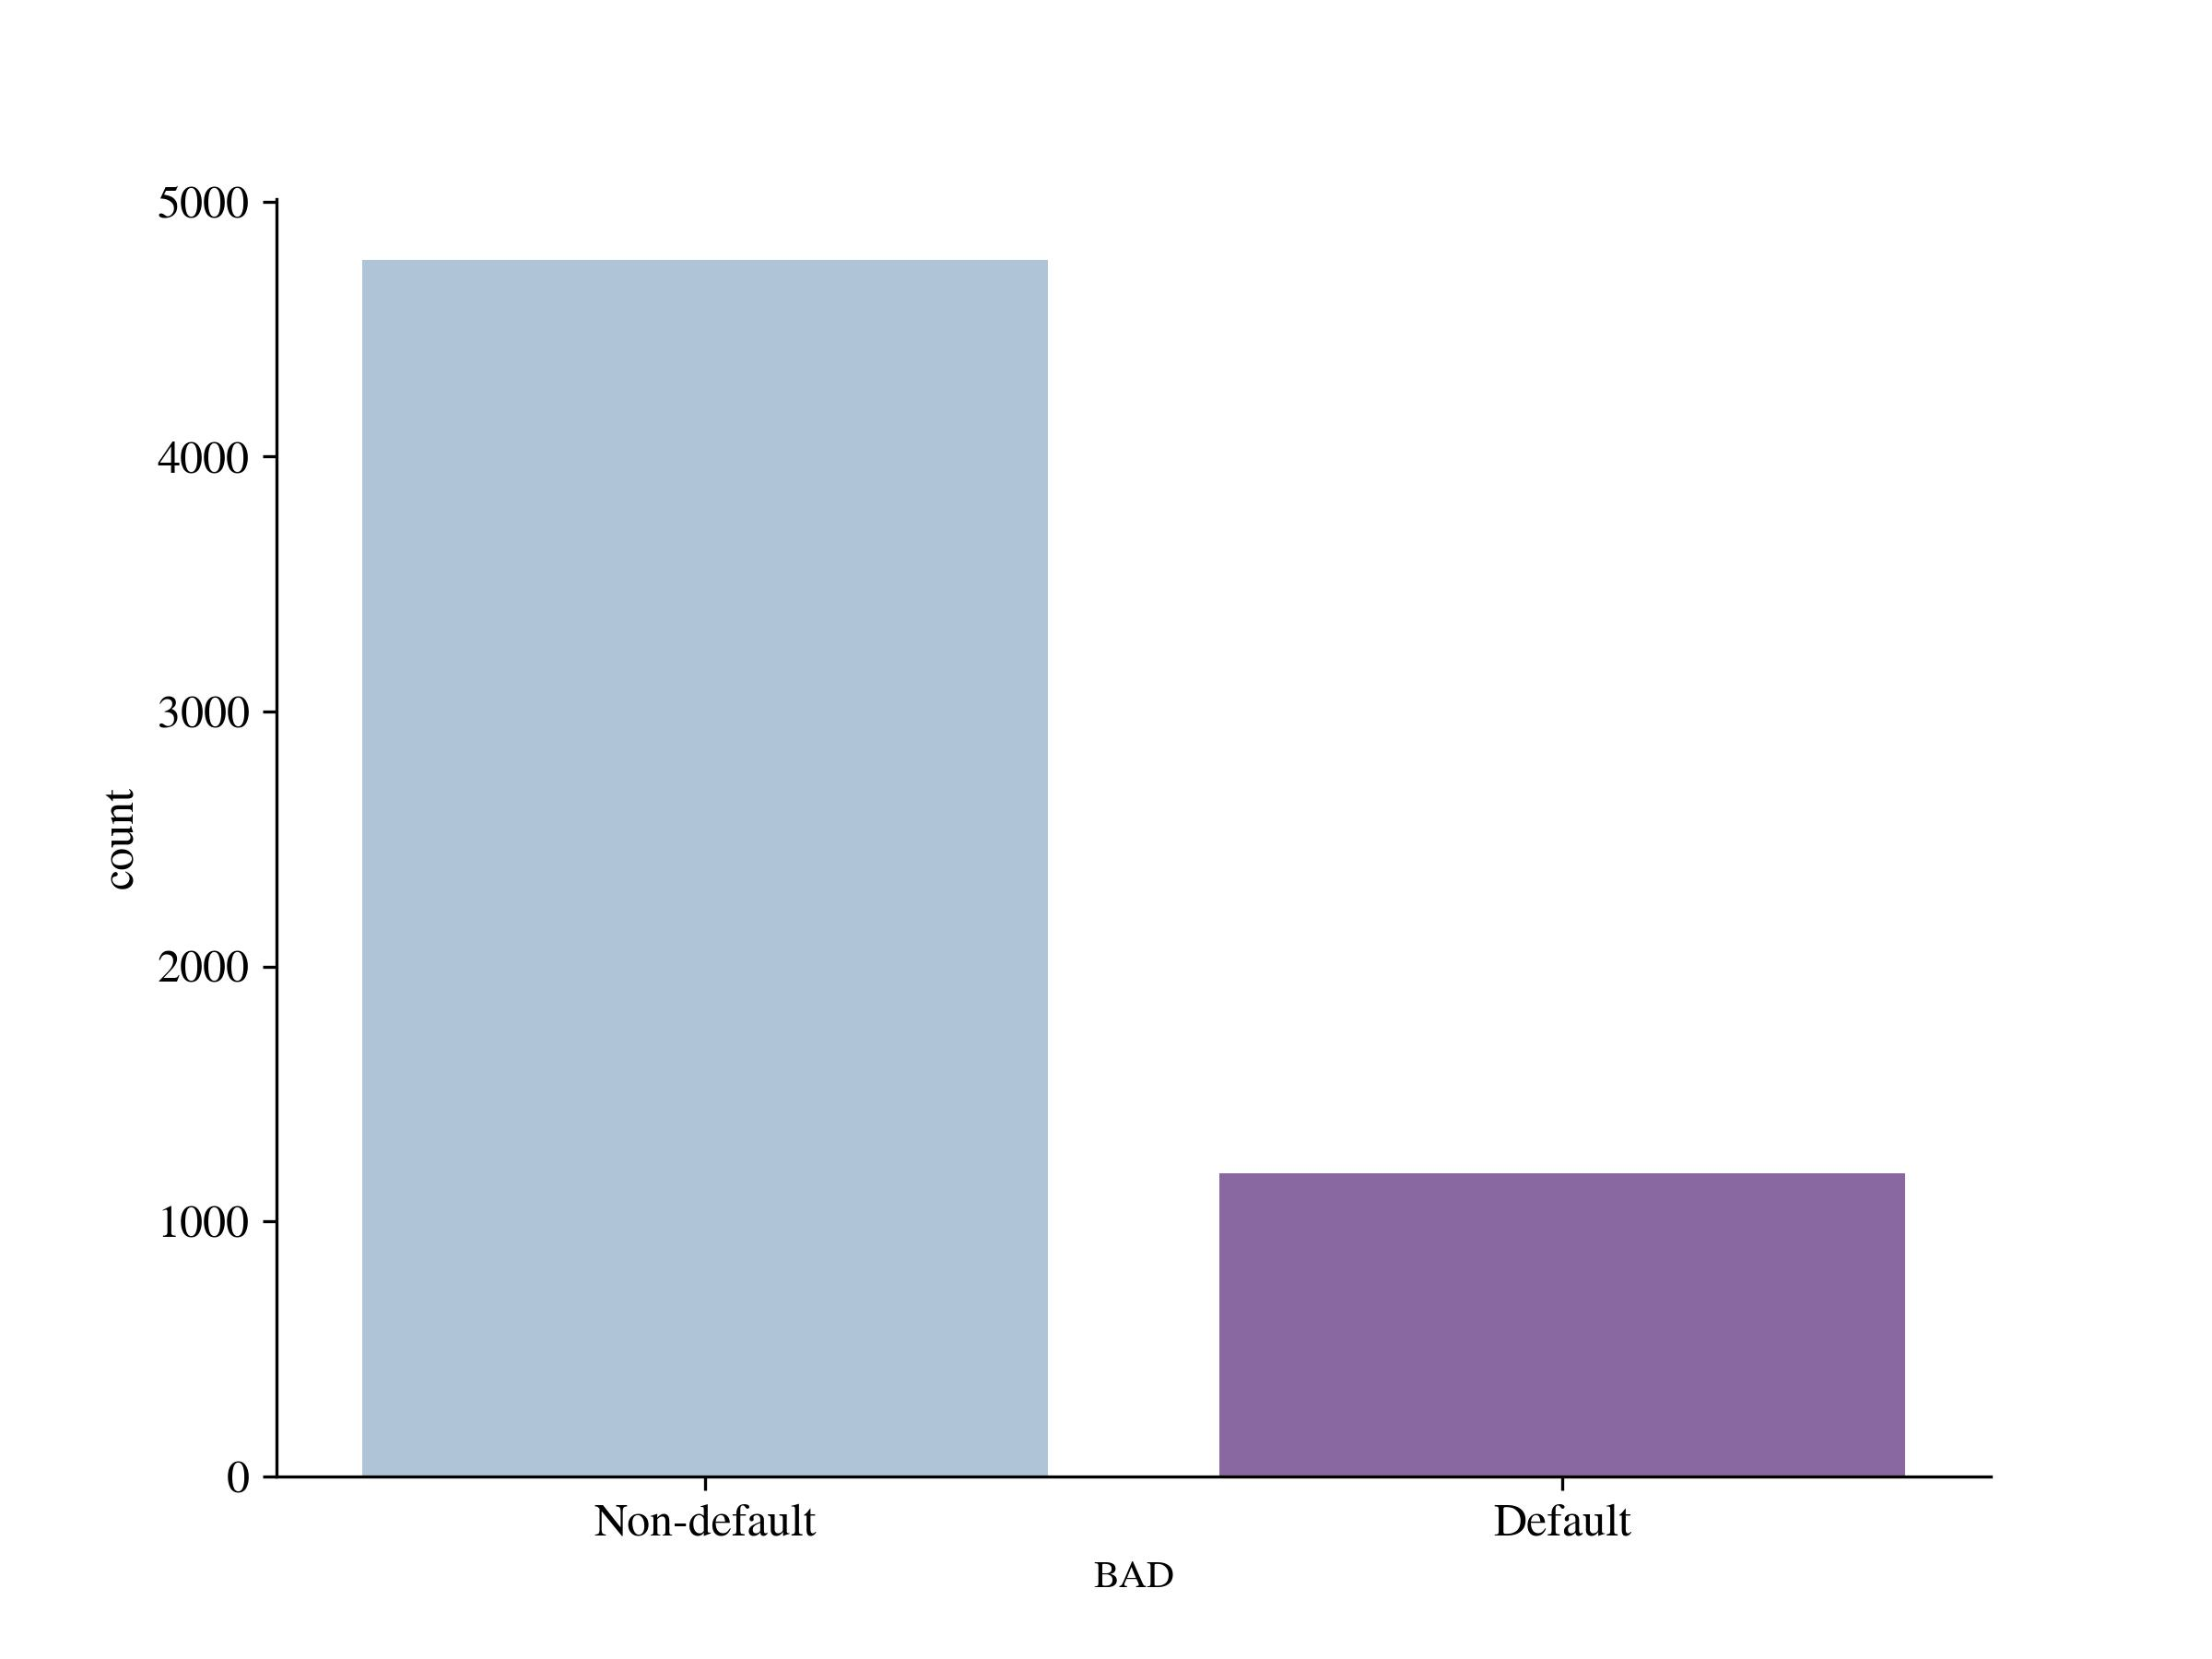
\includegraphics[width=130mm]{Figures/Default_Distribution.jpg}\vspace{-1em}
\centering{\begin{source}Author's results in Python\end{source}}\vspace{-1em}
\end{figure}

\subsubsection{Numeric Features' Distribution}
\label{subsubsec:numdist}

Regarding the numeric features, it can be observed that most of them exhibit a positive skewness and contain outliers, as illustrated in \autoref{fig:boxfeat}, which depicts the conditional distribution of the numeric features with respect to the default status via boxplots.

All the outliers appear to be valid, indicating that they have not arisen due to data entry errors.
This can be attributed to the non-negative nature of all the numeric features, which makes it impossible to have negative values for features such as the number of years at present job or the number of delinquent credit lines, among others.
Additionally, the maximum values of the given features are not unrealistically high, further corroborating the validity of the outliers.
However, it is necessary to treat these outliers as they can bias a model's weights or coefficients, particularly in the case of logistic regression or neural networks.
Outliers can also jeopardize distance calculations in the case of KNN, or in general, affect the position and orientation of the decision boundary.
Such factors can lead to overfitting and inaccurate and biased predictions.
A detailed explanation of the outlier treatment is provided in \autoref{subsec:prep-optbinning}.

Concerning the target variable, it can be observed that there are some differences in the distribution shapes of \texttt{DEROG} and \texttt{DELINQ}, which exhibit less skewness and lower dispersion for non-default cases as compared to default cases.
Since both features indicate negative information about delinquency, it is expected that a higher value for these features would increase the likelihood of loan default.
Referring to the feature \texttt{DEBTINC}, it does not exhibit any extreme values for non-default cases, but some extreme values are present for default cases.
From this, it can be inferred that if the debt-to-income ratio is too high, indicating that the applicant's income is not sufficient to cover their debt, the loan is more likely to end in default.
The association between the default status and the numeric features is further investigated in \autoref{subsubsec:target-num-ass}.

\begin{figure}[H]
\centering
\caption{Conditional distribution of numeric features}\vspace{0.5em}
\label{fig:boxfeat}
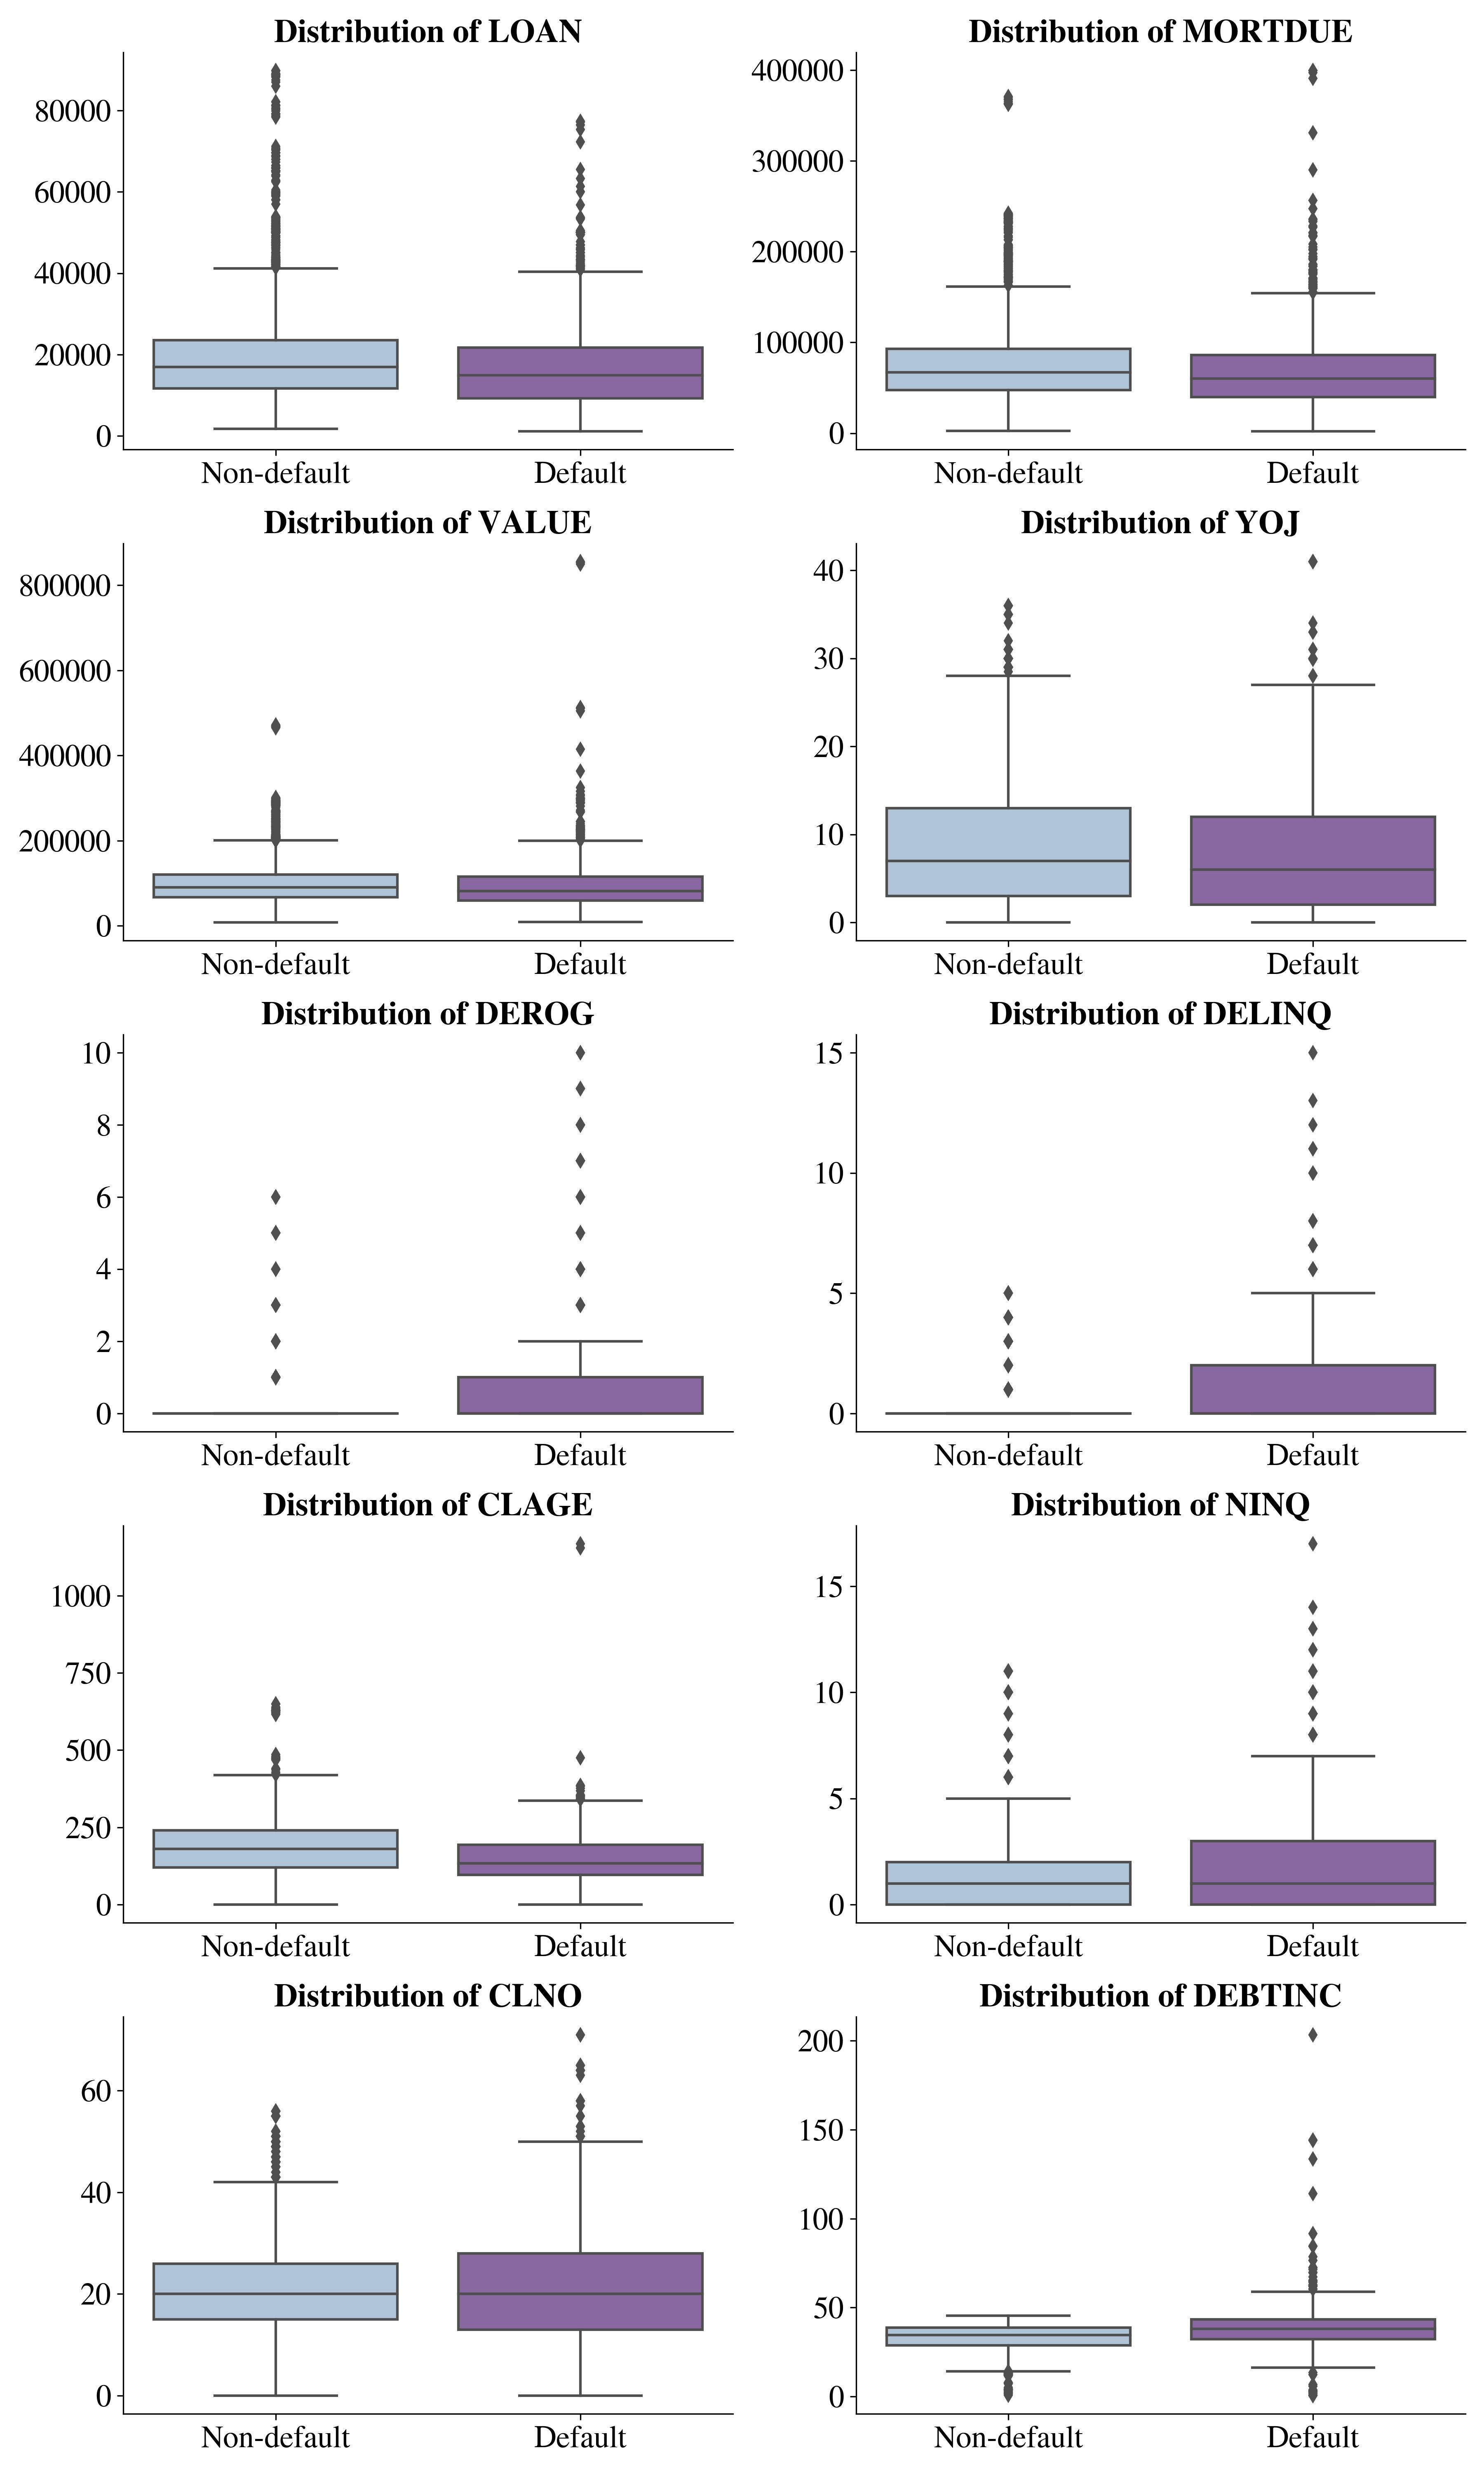
\includegraphics[width=140mm]{Figures/Numeric_Features_Distribution_Boxplots.jpg}
\centering{\begin{source}Author's results in Python\end{source}}\vspace{-1em}
\end{figure}

Due to the fact that the boxplots do not capture the missing values occurred in given features, it is also important to inspect the numbers and proportions of missing values in each feature, conditional on the default status.
As can be seen in \autoref{tab:nacont-table}, $n_0$ refers to the number of missing values in given feature for non-default cases, $n_1$ refers to the number of missing values in given feature for default cases.
$N_0$ and $N_1$ refer to the total number non--default cases and default cases respectively, therefore $n_0/N_0$ refers to the proportion of missing values in given feature for non-default cases, and $n_1/N_1$ refers to the proportion of missing values in given feature for default cases.

Pertaining to the feature \texttt{DEBTINC}, we can observe a significant difference in the number of missing values between the default and non-default cases. Out of all defaulted loans, 66.11 \% had missing debt--to--income ratio, whereas only 10.08 \% out of all non-defaulted loans had missing debt--to--income ratio.
Therefore, there could be a strong association between the missing debt--to--income ratio and the default.

Similarly, the table depicts a significant difference with respect to \texttt{VALUE} as 0.15 \% had missing collateral property value out of all non--defaulted loan, and 8.92 \% defaulted loans had missing collateral property value.
It can be inferred that loan applicants who withhold information on their collateral property value or debt-to-income ratio are more likely to default on their loans.
This may be due to negative information that they are trying to conceal, such as an excessively high debt or low income, or a low collateral property value.
Such associations are further investigated in \autoref{subsubsec:target-na-ass}.


\begin{table}[H]
\small
\setlength{\tabcolsep}{8pt}
\renewcommand{\arraystretch}{1.3}
% define a new column type 'L' for left alignment
\newcolumntype{R}[1]{>{\raggedleft\arraybackslash}p{#1}} % define a new column type 'R' for right alignment
\begin{center}
\caption[Numeric features NA's table]{Numeric features NA's table}\label{tab:nacont-table}
\begin{tabular}{l R{1cm}R{1cm}|R{1.5cm}R{1.5cm}}
    \toprule
    \textbf{Feature} & \textbf{$n_0$} & \textbf{$n_1$} & \textbf{$n_0/N_0$} & \textbf{$n_1/N_1$} \\
    \midrule
    \hline
    LOAN & 0 & 0 & 0 \% & 0 \% \\

    MORTDUE & 412 & 106 & 8.64 \% & 8.92 \% \\

    VALUE & 7 & 105 & 0.15 \% & 8.83 \% \\

    YOJ & 450 & 65 & 9.43 \% & 5.47 \% \\

    DEROG & 621 & 87 & 13.02 \% & 7.32 \% \\

    DELINQ & 508 & 72 & 10.65 \% & 6.06 \% \\

    CLAGE & 230 & 78 & 4.82 \% & 6.56 \% \\

    NINQ & 435 & 75 & 9.12 \% & 6.31 \% \\

    CLNO & 169 & 53 & 3.54 \% & 4.46 \% \\

    DEBTINC & 481 & 786 & 10.08 \% & 66.11 \% \\ \hline
    \bottomrule
\end{tabular}
\end{center}
\begin{center}
\source{Author's results in Python}
\end{center}
\end{table}
\subsubsection{Categorical Features' Distribution}
\label{subsubsec:catdist}

Regarding the distribution of categorical features, the dataset includes 2 nominal features, namely \texttt{REASON} and \texttt{JOB}.
The conditional distribution of categorical features on the default status is visualized using barplots in \autoref{fig:catdist}.
The plot indicates that most loan applicants applied for debt consolidation, while most job occupancies were labeled as \texttt{Other}.

With respect to the default status, there appears to be no significant difference between the default and non-default cases in terms of the relative distribution of the \texttt{REASON} feature.
However, a slight difference is observed between the default and non-default cases in terms of the relative distribution of the \texttt{JOB} feature.
Specifically, the categories \texttt{Office}, \texttt{ProfExe}, and \texttt{N/A} exhibit a relatively higher proportion of non-default cases than default cases.
Hence, a moderate association between the \texttt{JOB} feature and the default status is possible, as further investigated in \autoref{subsubsec:target-cat-ass}.


\begin{figure}[H]
\centering
\caption{Conditional distribution of categorical features}\vspace{0.5em}
\label{fig:catdist}
\includegraphics[width=140mm]{Figures/Categorical_Features_Distribution.jpg}
\centering{\begin{source}Author's results in Python\end{source}}\vspace{-1em}
\end{figure}
\subsection{Association Analysis}
In this subsection, we aim to examine potential relationships between the variables by analyzing their associations. Firstly, we investigate the association between the default status and the features. Subsequently, we explore the association among the features themselves.

\subsubsection{Association between default status and numeric features}
\label{subsubsec:target-num-ass}

To measure the association between the target variable and the numeric features, we use the Point-Biserial correlation coefficient, which is the Pearson's product moment correlation coefficient between a continuous variable and a dichotomous variable \citep{kornbrot2014point}.
This coefficient ranges from -1 to +1 and can be used to assess the strength and direction of the relationship between a continuous variable and a binary variable.
The formula for computing this coefficient is as follows:

\begin{equation}\label{eq}
r_{pb,X} =  \frac{\mu \left( X | Y=1 \right) -\mu \left( X | Y=0 \right)}{\sigma_{X}}\sqrt{\frac{N\left(Y=1\right) \times N\left(Y=0\right)}{N \left(N - 1 \right)}}
\end{equation}

Here, $\mu \left( X | Y=1 \right)$ and $\mu \left( X | Y=0 \right)$ represent the means of the given numeric feature $X$ conditional on the default status and non-default status, respectively, while $\sigma_{X}$ denotes the standard deviation of $X$.
The values of $N\left(Y=1\right)$ and $N\left(Y=0\right)$ indicate the number of observations with default status and non-default status, respectively, and $N$ represents the total number of observations within the feature $X$.


The following \autoref{tab:pointbi} displays the computed Point-Biserial coefficient for each numeric feature with respect to the default status, along with its statistical significance.
The results show that features such as \texttt{DEROG}, \texttt{DELINQ}, and \texttt{DEBTINC} are moderately and positively associated with the default status at the 1\% statistical significance level.
These findings support the observations made in \autoref{subsubsec:numdist} regarding the positive associations of these features with the default status. It can be inferred that these features may serve as important predictors in the model.

\begin{table}[H]
    \small
    \setlength{\tabcolsep}{8pt}
    \renewcommand{\arraystretch}{1.3}
    \centering
        \caption[Point--Biserial Correlation table]{Point--Biserial Correlation table}\label{tab:pointbi}
        \begin{tabular}{@{} l r @{\hspace{1cm}} l @{}}
    \toprule
    \textbf{Feature} & \textbf{Coefficient} & \textbf{Significance}\\
    \midrule
    \hline

    LOAN & -0.075  & ***\\

    MORTDUE & -0.048  & ***\\

    VALUE & -0.030  & ** \\
    
    YOJ & -0.060  & *** \\

    DEROG & 0.276 & *** \\

    DELINQ & 0.354 & *** \\
    
    CLAGE & -0.170 & *** \\

    NINQ & 0.175 & *** \\

    CLNO & -0.004 & \\

    DEBTINC & 0.200 & *** \\
    \hline
    \bottomrule
    \end{tabular}
    \vspace{0.35em}


        \centering\footnotesize{$^{*}$: $p<0.10$, $^{**}$: $p<0.05$, $^{***}$: $p<0.01$}\vspace{0.7em}

        \centering{\begin{source}Author's results in Python\end{source}}\vspace{-1em}

\end{table}

\subsubsection{Association between default status and categorical features}
\label{subsubsec:target-cat-ass}

In order to measure the strength of the relationship between the dichotomous default status and categorical variables, we employ Cramer's V, which ranges from 0 to 1 and is defined as:


\begin{equation}\label{eq}
    CV_{X} = \sqrt{\frac{\chi^{2}}{N\left(k-1\right)}}
\end{equation}


As noted in \autoref{subsubsec:catdist}, the association between the default status and \texttt{REASON} is weak, as evidenced by the Cramer's V value being close to zero.
Conversely, the association between the default status and \texttt{JOB} is slightly stronger, as the categories \texttt{Office}, \texttt{ProfExe}, and \texttt{N/A} exhibit a higher proportion of non-default cases than default cases.
Both \texttt{REASON}'s and \texttt{JOB}'s associations with default status are statistically significant at the 1\% significance level.

While statistical significance is important, it does not necessarily indicate that a feature is a strong predictor of the target variable.
Ultimately, the usefulness of a feature in predicting the target variable is determined by the performance metrics of the model.

    \begin{table}[H]
        \small
        \setlength{\tabcolsep}{8pt}
        \renewcommand{\arraystretch}{1.3}
        \centering
            \caption[Cramer's V Association table]{Cramer's V Association table}\label{tab:cramer-v}
            \begin{tabular}{@{} l r @{\hspace{1cm}} l @{}}
        \toprule
        \textbf{Feature} & \textbf{Coefficient} & \textbf{Significance}\\
        \midrule
        \hline
        REASON & 0.038  & ***\\
        JOB & 0.120  & ***\\
        \hline

        \bottomrule
    \end{tabular}
    \vspace{0.35em}


        \centering\footnotesize{$^{*}$: $p<0.10$, $^{**}$: $p<0.05$, $^{***}$: $p<0.01$}\vspace{0.7em}

        \centering{\begin{source}Author's results in Python\end{source}}\vspace{-1em}
\end{table}

\subsubsection{Association between default status and missing values}
\label{subsubsec:target-na-ass}

Given that the loan dataset contains missing values, it is necessary to examine whether the missingness is associated with the default status. One possible approach is to encode the feature with missing values as a binary variable, where 1 indicates the presence of a missing value and 0 otherwise.

To quantify the strength of association between the two binary variables, the Phi coefficient is used, which is defined as:

\begin{equation}\label{eq}
\phi_{X} = \sqrt{\frac{\chi^{2}}{n}}
\end{equation}

In line with the finding regarding the \texttt{DEBTINC} and \texttt{VALUE} in \autoref{subsubsec:numdist}, there is a strong and statistically significant association between the missing debt-to-income ratio and default status, and a moderate and statistically significant association between the missing collateral property value and default status, as shown in \autoref{tab:phi-target}.
Therefore, we can anticipate that these features will be crucial indicators in default prediction. Further details on feature selection are presented in \autoref{subsec:feature-selection}.
\begin{table}[H]
    \small
    \setlength{\tabcolsep}{8pt}
    \renewcommand{\arraystretch}{1.3}
    \centering
        \caption[Phi Correlation Coefficient table]{Phi Correlation Coefficient table}\label{tab:phi-target}
        \begin{tabular}{@{} l r @{\hspace{1cm}} l @{}}
    \toprule
    \textbf{Feature} & \textbf{Coefficient} & \textbf{Significance}\\
    \midrule
    \hline
    LOAN & 0.000  & \\
    \hline
    MORTDUE & 0.003  & \\
    \hline
    VALUE & 0.254  & *** \\
    \hline
    REASON & 0.004 & \\
    \hline
    JOB & 0.064 & *** \\
    \hline
    YOJ & 0.056  & *** \\
    \hline
    DEROG & 0.070 & *** \\
    \hline
    DELINQ & 0.061 & *** \\
    \hline
    CLAGE & 0.030 & ** \\
    \hline
    NINQ & 0.039 & *** \\
    \hline
    CLNO & 0.018 & \\
    \hline
    DEBTINC & 0.547 & *** \\
    \bottomrule
    \end{tabular}
    \vspace{0.35em}


        \centering\footnotesize{$^{*}$: $p<0.10$, $^{**}$: $p<0.05$, $^{***}$: $p<0.01$}\vspace{0.7em}

        \centering{\begin{source}Author's results in Python\end{source}}\vspace{-1em}
\end{table}

\subsubsection{Missing Values Association}
Additionally, it is imperative to investigate the relationship between missing values and default status, as well as the interrelationship between the missing values themselves.
A common approach to identifying patterns of missing data in a dataset is through the use of a dendrogram, which clusters variables hierarchically based on the occurrence of missing values.
This method groups variables into clusters based on the similarity of their missing value patterns, such that variables with comparable patterns of missingness are clustered together.
Conversely, variables with dissimilar patterns of missingness are placed in separate clusters.
The dendrogram is constructed by merging the two closest clusters iteratively until all variables are in the same cluster.
The distance between the clusters at each step of the merging process is shown on the y-axis of the dendrogram, and the order in which the variables are merged is displayed on the x-axis.

In \autoref{fig:dendrogram}, the hierarchical clustering of the dataset's variables is illustrated, excluding the default status and requested loan amount feature \texttt{LOAN}, as these variables do not contain any missing values.
As depicted in the dendrogram, the \texttt{CLNO} and \texttt{CLAGE} features have the most similar patterns of missing values occurrences.
Therefore, it can be inferred that a significant number of loan applicants tend to omit information regarding their number of credit lines (\texttt{CLNO}) and the age of their most recent credit line (\texttt{CLAGE}) when submitting their loan applications.

\begin{figure}[H]
    \centering
    \caption{Nullity dendrogram}\vspace{0.5em}
    \label{fig:dendrogram}
    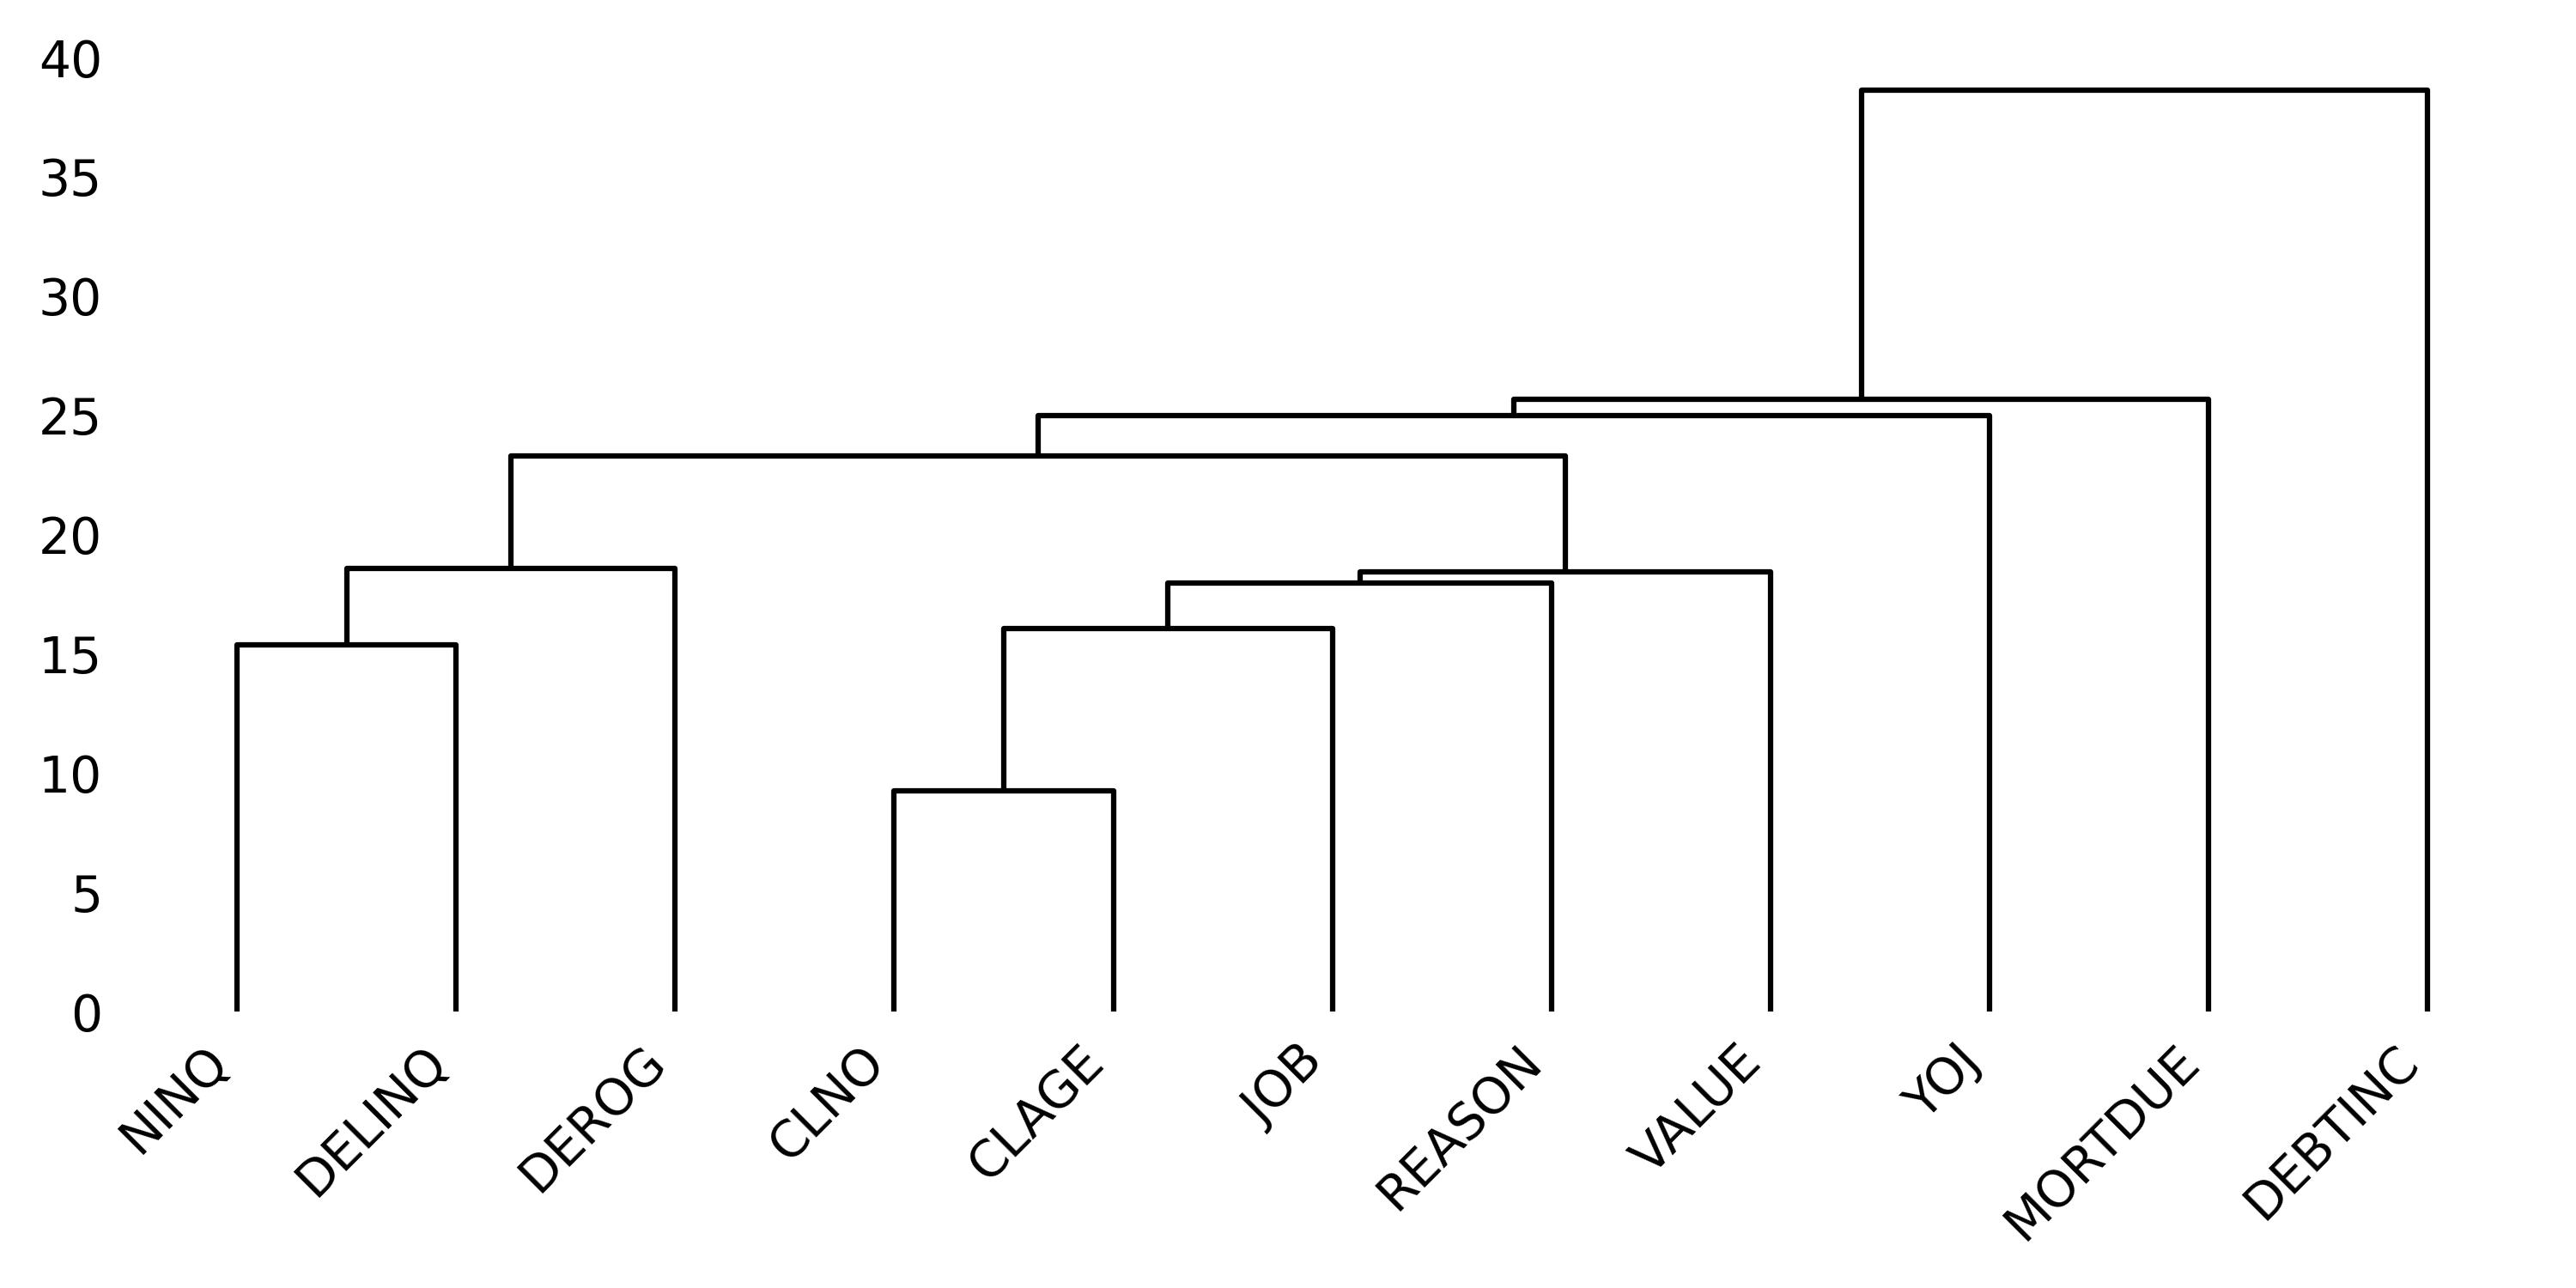
\includegraphics[width=150mm]{Figures/NA_Dendrogram.jpg}
    \centering{\begin{source}Author's results in Python\end{source}}\vspace{-1em}
\end{figure}

\subsubsection{Multicolinearity Analysis}

To quantify the association between the numerical features, Pearson correlation coefficient is often used.
However, it is highly sensitive to outliers and makes assumptions regarding the normal distribution and linear relationship between variables.
Consequently, Spearman correlation coefficient is utilized as an alternative, as it is a non-parametric measure that does not make any assumptions regarding the distribution of variables or the linearity of their relationship.
The Spearman correlation coefficient is defined as follows:

\begin{equation}\label{eq}
\rho_{spearman} = 1 - \frac{6 \sum_{i=1}^{n} d_{i}^{2}}{n \left(n^{2}-1\right)}
\end{equation}


In the \autoref{fig:spearmancorr}, we can observe a very strong correlation between the \texttt{MORTDUE} and \texttt{VALUE} features. Such multicolinearity can cause problem in predictions na model's overfitting. Therefore, a feature selection is recommended - such selection is further described in \autoref{subsec:feature-selection}.

\begin{figure}[H]
    \centering
    \caption{Spearman Correlation Matrix}\vspace{0.5em}
    \label{fig:spearmancorr}\
    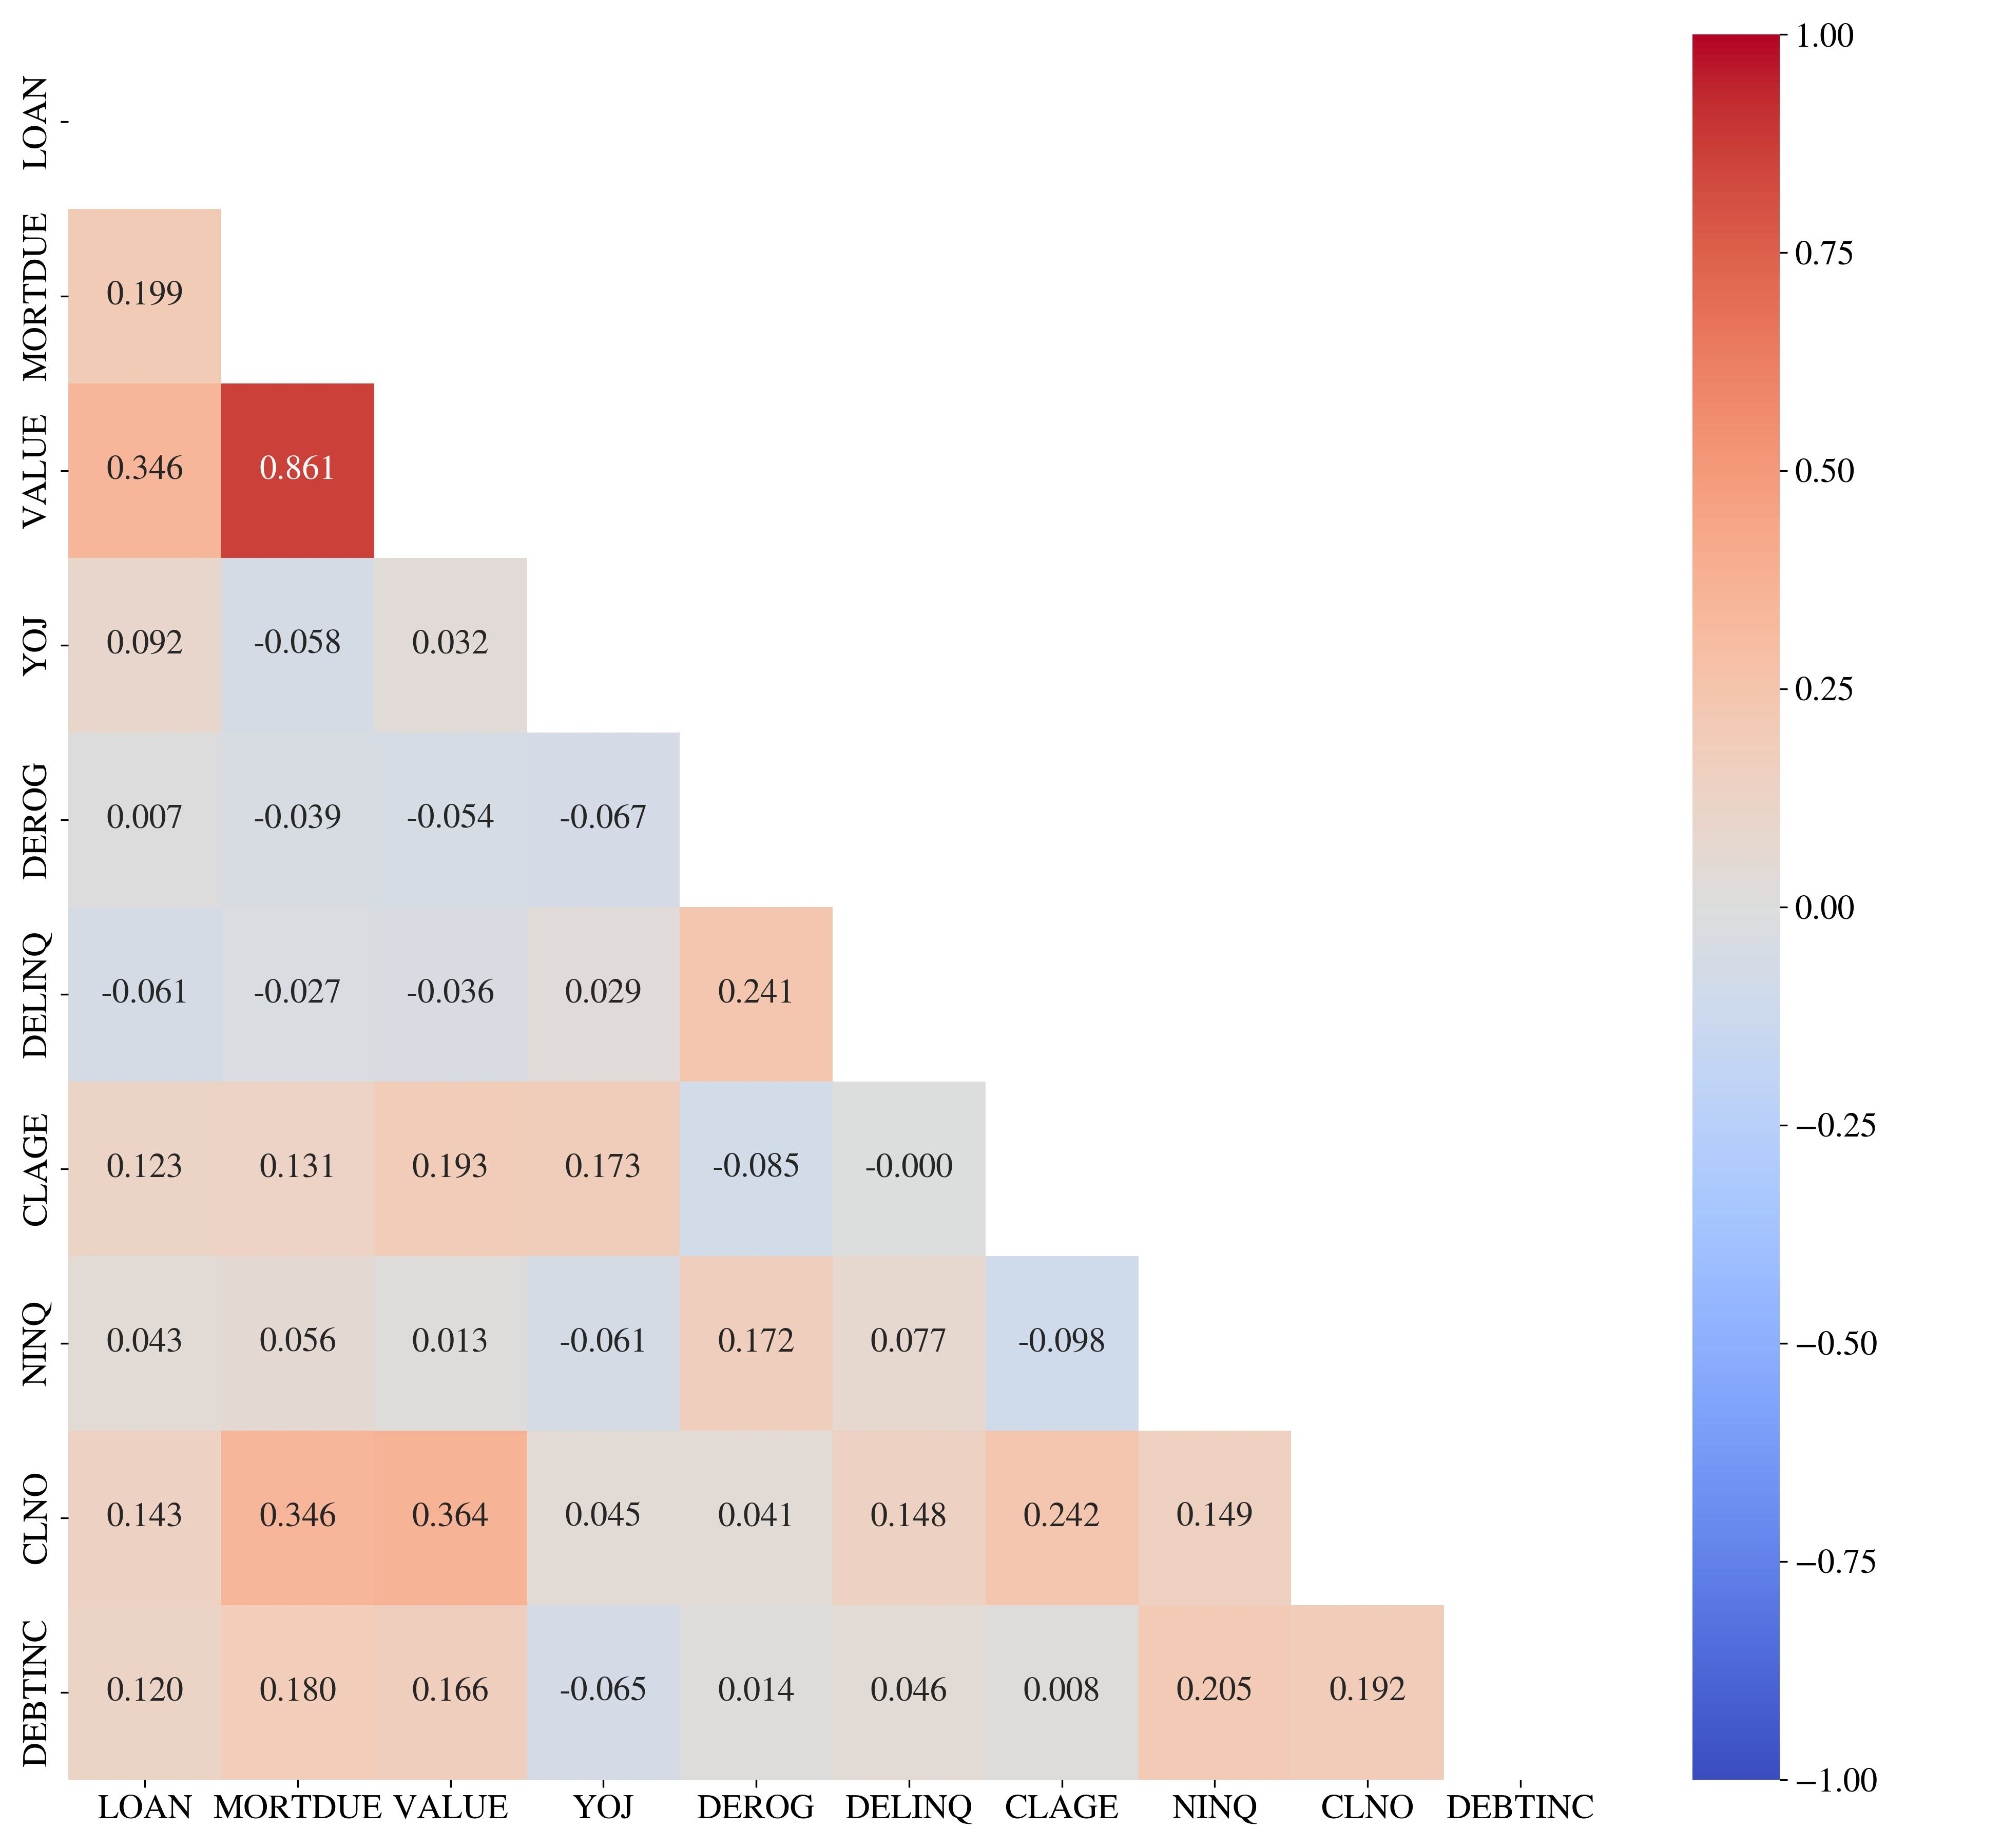
\includegraphics[width=150mm]{Figures/Spearman_Correlation_Matrix_Numeric_Features.jpg}
    \centering{\begin{source}Author's results in Python\end{source}}\vspace{-1em}
\end{figure}


\section{Data Preprocessing}
In this section, the process of preprocessing data is described as the crucial step in the machine learning modelling. Particularly, the following is described:
\begin{itemize}\setlength\itemsep{0em}
\item Splitting the data
\item oversampling,
\item discretization,
\item Weight--of--Evidence encoding.
\end{itemize}


\subsection{Data Split and ADASYN Oversampling}
\label{subsec:data-split-ADASYN}

To ensure appropriate model training and unbiased evaluation, it is necessary to split data into separate sets for various purposes. Specifically, the data was split into three sets with the ratio of 70:15:15:
\begin{itemize}\setlength\itemsep{0em} 
\item Training set for model training, feature selection, and hyperparameter tuning;
\item Validation set for selecting the best final model;
\item Test set for the final evaluation of the best final model.
\end{itemize}

The data is split using stratified split to preserve the default status distribution, which was highly imbalanced.
Stratification ensures that the distribution of defaults and non-defaults remains the same across all sets, thereby avoiding overfitting and data leakage. Using stratification, each set had 80 \% non-defaults and 20 \% defaults. This method enables accurate prediction since the model is trained and evaluated on the same population \citep{igareta2021strat}.

\subsubsection{ADASYN Oversampling}

However, stratification alone may not be sufficient for dealing with imbalanced classes. One would use random undersampling or random oversampling to deal with the class imbalanced issue. The former randomly eliminates majority class instances whereas the latter randomly duplicates minority class instances.
However, both have particular drawbacks, as the random under-sampling may lead to a a significant loss of information, and random oversampling is lead to the high degree of repetation of minority instances. Both then could lead to model's overfitting and detoriation in model's performance \citep{ma2013imbalanced}.
This might be a significant issue when the target variable distribution is heavily imbalanced - assume that we have a dataset of 1,000 instances where 990 instances belongs to majority class and 10 instances to minority class.
If we perform random undersampling in order to balance the target variable distribution, we would have to remove 980 instances and end up with undersampled dataset of 20 instances, which is not acceptable for model training.
On the other hand, if we perform random oversampling, we would end up with 1,980 instances, where 980 instances would be the same as in the original dataset, which would lead to the model's overfitting.

Therefore, the Adaptive Synthetic Sampling (henceforth ADASYN) technique is used for oversampling the minority class.
ADASYN generates synthetic instances of the minority class based on the nearest neighbors of the minority class instances.
Such approach is more effective than Synthetic Minority Oversampling Technique (henceforth SMOTE) which also uses nearest neighbors to generate synthetic instances of minority class, as it generates more synthetic instances which are hard--to--learn by K-Nearest Neighbors given the density distributtions, whereby SMOTE generates synthetic instances uniformly for each minority instance.
 \citep{adasynhaibo}. 
In other words, ADASYN generates more synthetic instances in regions where the density of the majority class within $K$ nearest neighbors of minority instance is higher and fewer synthetic instances in regions where the density is lower, thereby ADASYN focuses on generating more hard--to--learn minority instances.
Thereby, it makes easier for the machine learning model to learn the decision boundary between the minority and majority classes and boost the model's performance by focusing on hard--to--learn instances \citep{adasynhaibo}. 
The oversampling is performed on the training set only after the split to avoid data leakage and biased evaluation.

Before oversampling algorithm's execution, first we need to calculate the number of instances of minority class to be synthetically generated in order to balance the target variable distribution. The number of instances to be generated $G$ is calculated as follows:
\begin{equation}\label{eq}
    G = \left(m_{l} - m_{s}\right) \times \beta
\end{equation}
where $m_l$ is the number of majority class instances, $m_s$ is the number of minority class instances and $\beta$ indicates the desired ratio between the numbers of majority and minority class instances after oversampling.

Then for each minority class instance $x_i$, using K-nearest Neighbors with Euclidean distance calculate the ratio $r_i$ as:
\begin{equation}\label{eq}
   r_{i} = \frac{\delta_{i}} {K}
\end{equation}
where $\delta_{i}$ is the number of majority class instances within the $K$ nearest neighbors of $x_i$.
In such case, higher $r_i$ indicates dominance of the majority class in given specific neighbourhood of $x_i$ \citep{nian2018introduction}.
Subsequently, all the $r_i$ ratios are normalized as:
\begin{equation}\label{eq}
    \hat{r}_{i} = \frac{r{i}}{\displaystyle\sum_{i=1}^{m_{s}} r_{i}}
\end{equation}
In such way that sum of all the normalized $\hat{r}_i$ ratios is equal to 1. Hence, we can denote $\hat{r}_i$ as the density distribution.
\begin{equation}\label{eq}
    \sum_{i=1}^{m_{s}} \hat{r}_{i} = 1
\end{equation}

Finally, the oversampling process is initialized.
For each minority class instance $x_i$, calculate the number of instances to be synthetically generated based on the respective density distribution $\hat{r}_i$ and the total number of instances to be synthetically generated $G$. Thus, for the minority classes with higher density, it generates more synthetic instances, since those instances are hard--to--classify by the K-Nearest Neighbors.
\begin{equation}\label{eq}
    G_i = G \times \hat{r}_{i}
\end{equation}
Further, for each minority class instance $x$, generate $G_i$ synthetic instances $s_i$ as follows:
\begin{equation}\label{eq}
    s_i = x_i + \left(x_{zi} - x_{i} \right) \times \lambda
\end{equation}
where $x_{zi}$ represents the radnomly chosen minority class instance within the $K$ nearest neares neighbors for $x_i$, and $\lambda \in \left[0,1\right]$ is a random number.

The following \autoref{tab:split} shows the default distribution of the individual sets before and after oversampling. The training set after ADASYN oversampling was balanced, while the default distribution remained the same across the validation and test sets before and after oversampling, which is desirable due to stratification.

\begin{table}[H]
\small
\setlength{\tabcolsep}{8pt}
\renewcommand{\arraystretch}{1.3}
\centering
    \caption[WoE distribution]{WoE distribution}\label{tab:split}
    \begin{tabular}{lrrr}
\toprule
\textbf{Set} & \textbf{\# instances} & \textbf{\% defaults} & \textbf{\% non--defaults}\\
\midrule
\hline
Training & 4,171  & 19.95 \% & 80.05 \% \\
Training (oversampled) & 6,437 &  48.13 \% & 51.87 \% \\

Validation & 895 &  20.00 \% & 80.00 \% \\

Test & 894 &  20.00 \% & 80.00 \% \\
\hline
\bottomrule
\end{tabular}
\vspace{0.7em}

\centering{\begin{source}Author's results in Python\end{source}}\vspace{-1em}
\end{table}

In Python, the data are divided and oversampled using a custom function \lstinline{data_split()}.
This function first employs the \lstinline{train_test_split()} function from the \lstinline{scikit-learn} module to split the data into training, validation, and test sets with a stratification technique.
Next, the \lstinline{ADASYN()} class from the \lstinline{imblearn} module is used to oversample the training set. This is achieved by generating synthetic instances of the minority class based on the five nearest neighbors and Euclidean distance.

However, the \lstinline{ADASYN()} class from \lstinline{imblearn} is not designed to handle missing values or categorical features encoded as character. To overcome this limitation, the following approach is taken:
\begin{enumerate}\setlength\itemsep{0em} 
\item Separate the categorical and numeric features;
\item Impute the missing values with arbitrary values:
\begin{itemize}
\item Categorical features: string \lstinline{'N/A'};
\item Numeric features: number \lstinline{99999999999999} - such value is chosen since it is highly unlikely to be present in the dataset.
\end{itemize}
\item Convert the categorical features into dummy variables;
\item Join the numeric features with the dummy variables;
\item Perform the oversampling on the joined dataset;
\item Convert the dummy variables back into categorical features;
\item Retrieve back the missing values:
\begin{itemize}
\item Categorical features: replace string \lstinline{'N/A'} with \lstinline{np.nan};
\item Numeric features: for each feature $X$ if its value exceeds the original maximum value, then replace it with \lstinline{np.nan};
\end{itemize}
\end{enumerate}

\textbf{ADD IMPACT OF OVERSAMPLING ON FEATURES DISTRIBUTION}

\subsection{Optimal Binning and Weight--of--Evidence}
\label{subsec:prep-optbinning}

In the context of data preprocessing, it is crucial to consider the most appropriate feature transformation method that optimizes the performance of machine learning models.
Although common approaches such as dummy encoding, standardization, logarithmic transformation, and normalization are widely used, they may not always be suitable for a given dataset due to the presence of certain characteristics.
For instance, dummy encoding may not be suitable for categorical features with a large number of categories as it could lead to the curse of dimensionality.
Standardization may not be appropriate for features with a large number of outliers as it may result in a loss of information.
Similarly, logarithmic transformation may not be appropriate for features with a large number of zeros, and normalization may not be suitable for features with a significant number of outliers.

Therefore, alternative approaches such as discretization or binning are increasingly being used. Binning is a categorization process to transform a continuous variable into a small set of groups or bins \citep{zeng2014necessary}. This approach enables the identification of outliers within bins and reduce their impact, and additionally, it can capture missing values without requiring the removal or imputation of such values.
As a result, binning is a more flexible and versatile feature transformation method that can effectively handle different types of datasets and is particularly useful in cases where other methods may not be appropriate.

In this thesis, we employ the \lstinline{BinningProcess} from the \lstinline{optbinning} module in Python for an optimal binning of both numeric and categorical features with respect to the target variable, developed by Guillermo Navas--Palencia \citep{navas2020optimal}. 
This approach involves grouping the values of a continuous variable into discrete intervals, or "bins", based on their relationship with the target variable.
Similarly, for categorical features, the approach involves grouping the categories based on their relationship with the target variable.
In general, the optimal binning is solved by iteratively merging an initial granular discretization until imposed constraints are satisfied. Particularly, the optimal binning process consists of two phases - pre--binning process (for generating initial granular discretization) and subsequent optimization (for satisfying imposed constraints).
The former phase usually uses decision tree to generate initial split points to create pre--bins which are further merged while maximizing Information Value (also known as Jeffreys' divergence) while accounting for the constraints. \citep{navas2020optimal} Such constraints are:
\begin{itemize}\setlength\itemsep{0em} 
    \item Creation of separate bins for missing values: Since missing values can have a significant impact on the target variable, hence is important to create a separate bin for them.
    \item Minimum bin size constraint - at least 5 \% of the total number of instances: Such constraint ensures a bin's representativness.
    \item Each bin should have at least one instance of each target class: Application of such constraint allows to compute divergence measure.
\end{itemize}
Thus, the optimal binning process, the goal is the maximize discriminatory power among bins, i.e., divergence measure.
For more information about optimal binning, please refer to \citep{navas2020optimal}.

After the binning process, the bins as categorical values needed to be encoded into numeric values. The most common approach in credit risk modelling is Weight-of-Evidence (henceforth WoE) encoding. The WoE is a commonly used measure of the strength of association between a binary target variable and an independent variable.
According to Witzany \citep{witzany2017credit}, the WoE of categorical value $c$ can be expressed as the change between the overal log odds ratio and the log odds ratio given the value $c$, hence:
\begin{equation}\label{eq}
    WoE\left(c\right) = \ln\left(\operatorname{Pr}\left(c \mid Y = 0 \right) \right) - \ln\left(\operatorname{Pr}\left(c \mid Y = 1 \right) \right)
\end{equation}
Assuming feature $X$ and its respective bin $b_i$, thus $b_i \in X$, we can express WoE in terms of $b$ as follows:
\begin{equation}\label{eq}
    WoE_{X, b}= \ln \left(\frac{\Pr{\left(X = b\;\middle|\;Y = 0\right)}}{\Pr{\left(X = b\;\middle|\;Y = 1\right)}}\right)
\end{equation}
According to Navas--Palencia \citep{navas2020optimal}, the WoE for bin $i$ can be also computed as:
\begin{equation}\label{eq}
    WoE_{i} = \ln \left( \frac{r^{ND}_i / r^{ND}_T} {r^{D}_i / r^{D}_T}  \right)
\end{equation}
where $r^{ND}_i$ is the number of non--default instances in given bin $i$, $r^{D}_i$ is the number of default instances in the given bin $i$, $r^{ND}_T$ is the total number of non--default instances in whole sample and $r^{D}_T$ is the total number of default instances in whole sample.
Thus, positive WoE value is indicates larger distribution of non--defaults, i.e. higher likelihood of non--default, while negative WoE value indicates larger distribution of defaults, i.e., higher likelihood of default. 

The following \autoref{fig:woedist} depicts the distribution of Weight-of-Evidence (WoE) bins for each feature. It can be observed that binning captures either linear, non-linear, monotonic, or non-monotonic relationships between the default status and the numeric features in terms of WoE.
Regarding the \texttt{DELINQ} feature, a monotonic relationship can be observed, where the higher number of delinquent credit lines, the lower the WoE coefficient, indicating a larger distribution of defaults with respect to non-defaults in the given bin.
Thus, the higher the number of delinquent credit lines, the higher the likelihood of defaulting in terms of WoE.

A non-linear relationship can be observed with respect to the \texttt{YOJ} feature, where the WoE coefficient is positive for applicants who have recently started working at their new job (i.e., number of years at the present job is less than 1) and for applicants who have been working at their current job for a relatively long time (i.e., number of years at the present job is higher than 19).
Thus, applicants who have been working for a longer time have stable income and are more creditworthy and less likely to default.
Regarding applicants who have recently started working at their new job, it is possible that they are less likely to default since the \texttt{YOJ} feature does not capture the applicant's total number of years of work experience, but only the number of years at the present job.
Thus, in the given dataset, applicants who have recently started working at their new job have a relatively higher total number of years of work experience, making them more creditworthy and less likely to default. On the other hand, for applicants who have been working at their present job between 1 and 19 years, the WoE coefficient is negative.
This relationship seems to be complex and can be influenced by other factors not present in the dataset, such as the applicant's age, total number of years of work experience, education, etc.

Both numeric and categorical features contain a separate bin capturing missing values, which can be a useful indicator when training a model. This is evident in the \texttt{DEBTINC} feature, where the bin capturing missing values has the most negative WoE coefficient, indicating that there is a larger distribution of defaulters compared to non-defaulters.
This finding was already raised in \autoref{subsubsec:target-na-ass} in terms of the strong and statistically significant association between the default status and the missing values in \texttt{DEBTINC}.

However, inconsistencies can also be observed in terms of distributions from exploratory analysis and the WoE coefficient distributions.
One example pertains to the \texttt{Mgr} category in the \texttt{JOB} feature, where the WoE coefficient is substantially negative, indicating that among managers, there is a larger distribution of defaulters compared to non-defaulters.
However, this was not observed in the distribution analysis of categorical features (\autoref{subsubsec:catdist}), where the relative distributions conditional on the default status do not differ too much in terms of the \texttt{Mgr} category.
This is a result of ADASYN oversampling, which synthetically replicates minority instances, especially those instances that are hard-to-learn.
Hence defaulted loans that managers have applied for are difficult to learn, and ADASYN balances default distribution by generating default instances having \texttt{JOB} equal to \texttt{Mgr}, which results in an increase in the number of instances having \texttt{JOB} equal to \texttt{Mgr}, i.e., a larger distribution of defaulters in the \texttt{Mgr} bin, and therefore a negative WoE coefficient.

\begin{figure}[H]
\centering
\caption{WoE Bins Distribution}\vspace{0.5em}
\label{fig:woedist}
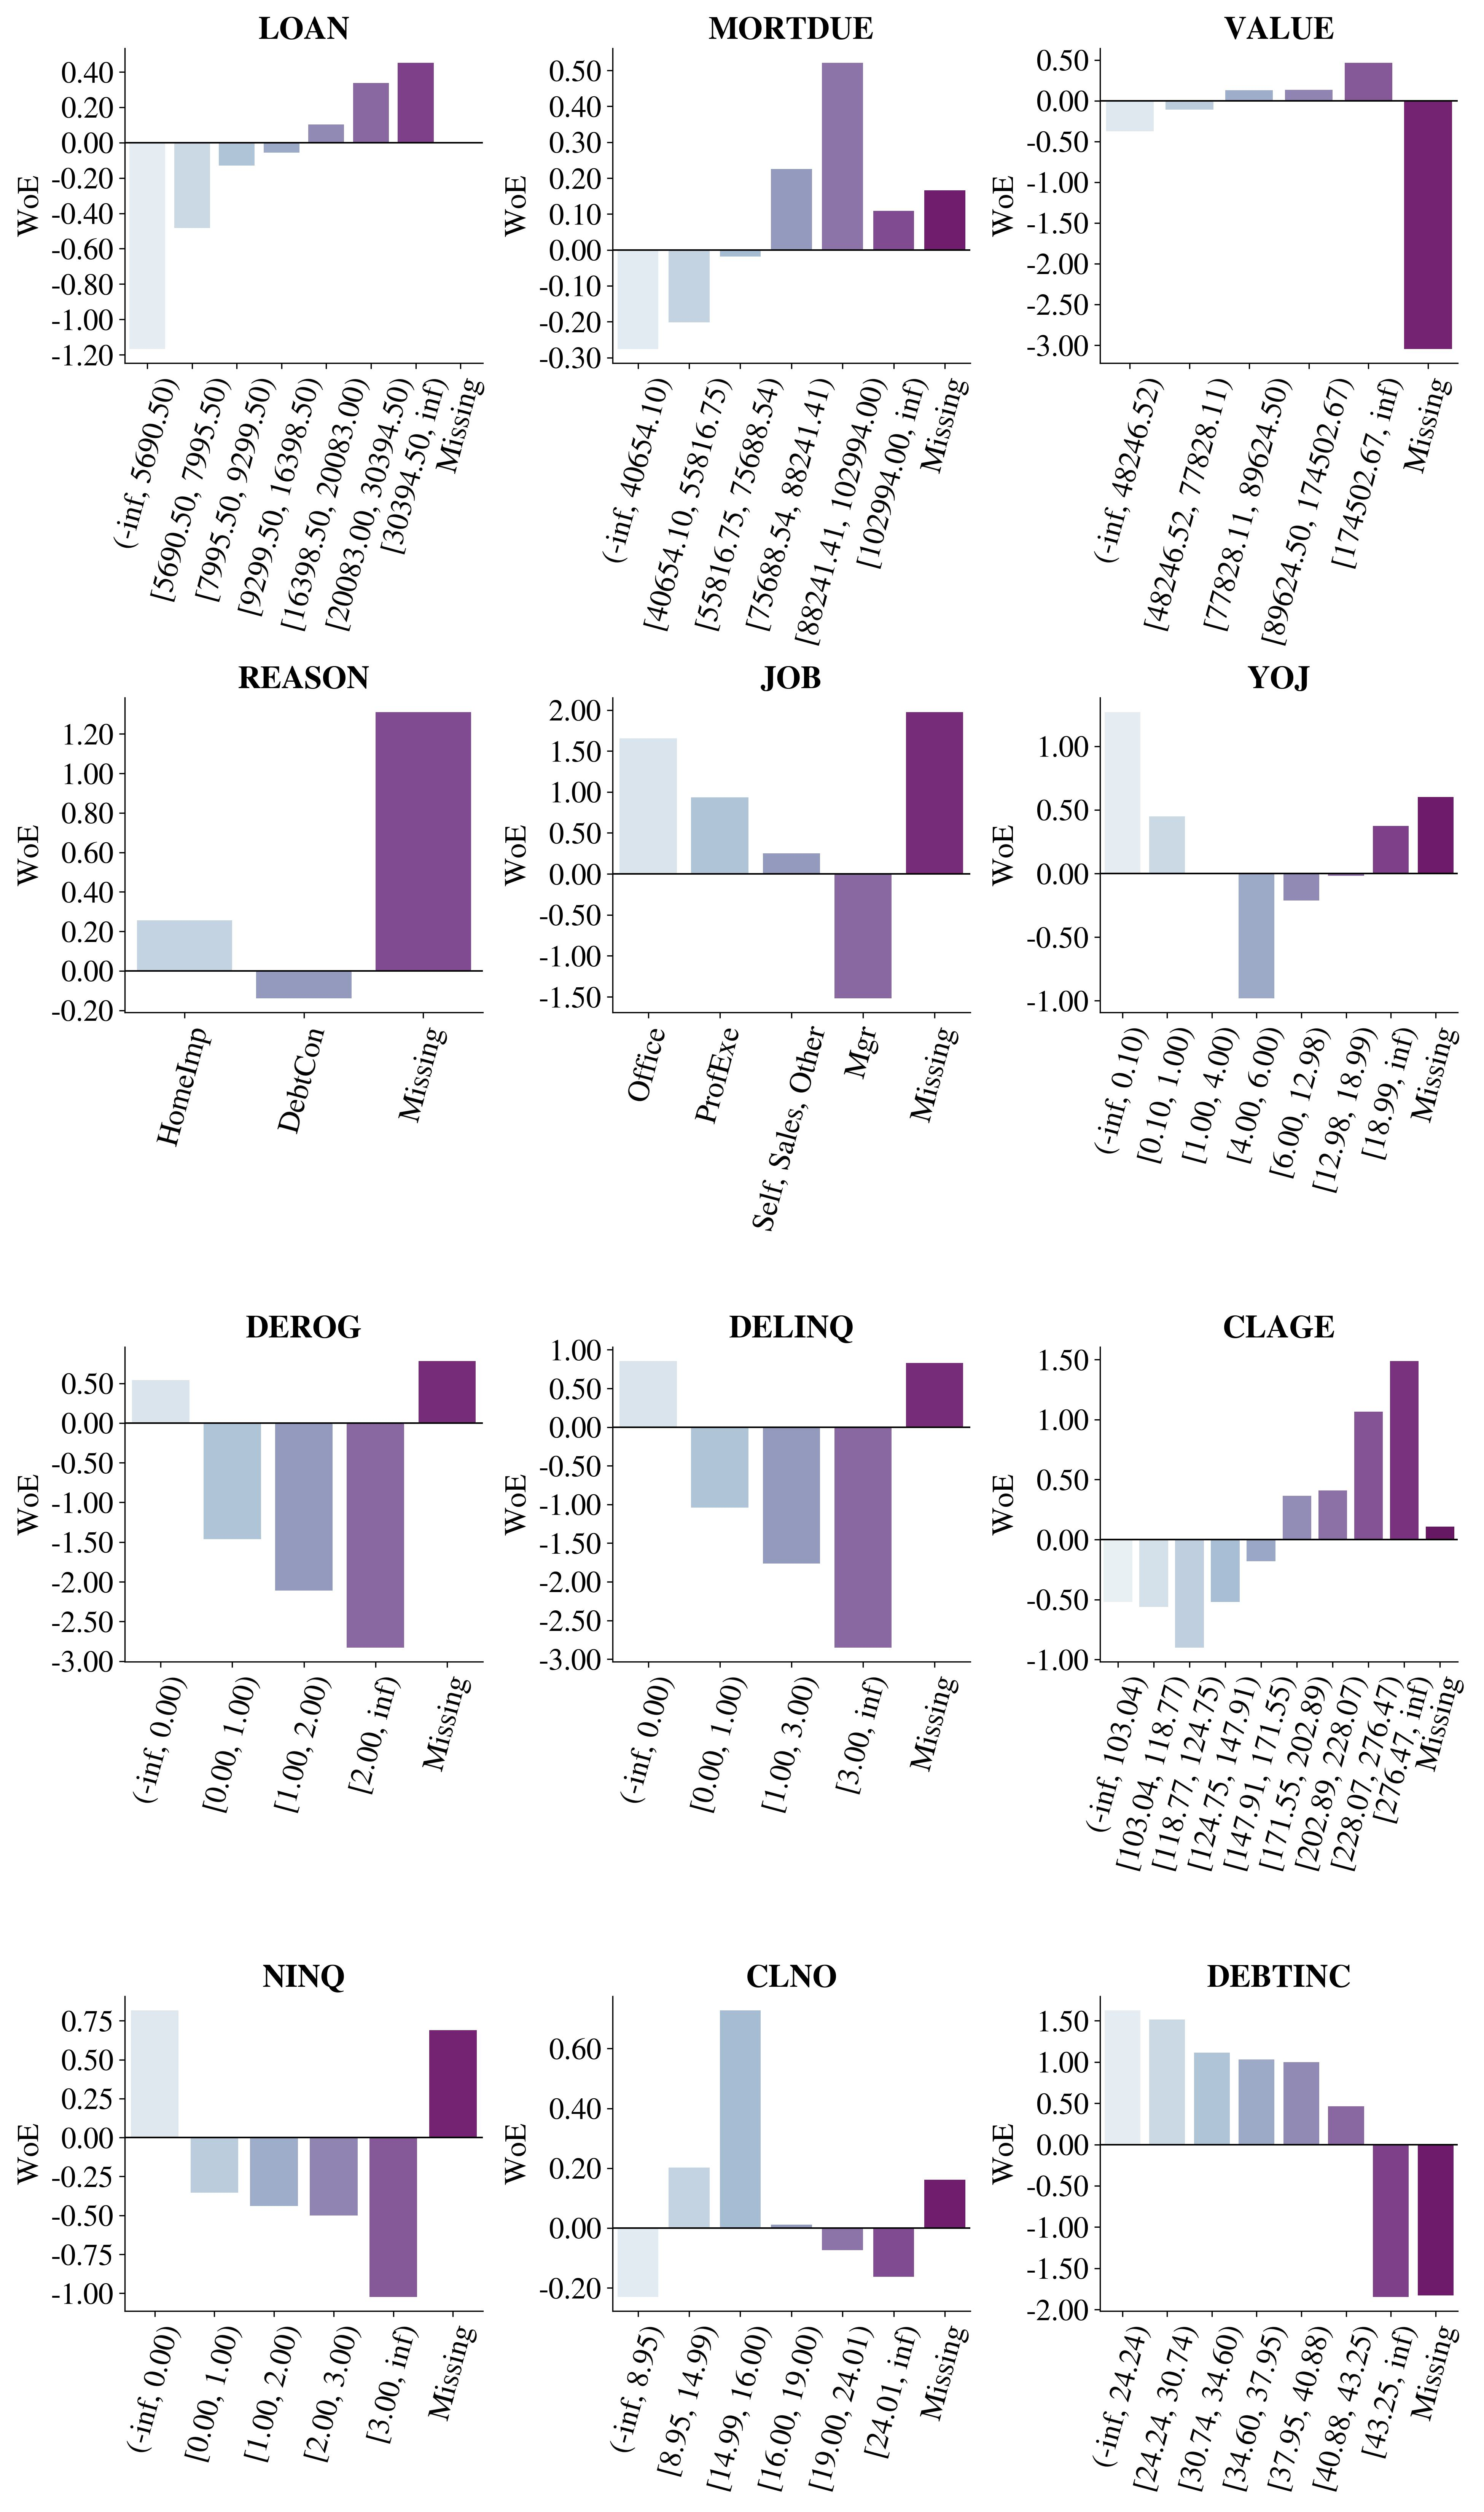
\includegraphics[width=140mm]{Figures/WoE_Distribution.jpg}
\centering{\begin{source}Author's results in Python\end{source}}\vspace{-1em}
\end{figure}


\section{Modelling}
Once the data are finally preprocessed, the next step regards the modelling part which includes hyperparameter tuning, feature selection, model selection and model building.

In Python, 8 different machine learning models from \lstinline{Scikit-learn} module are used for the default status prediction, which were already described in \autoref{sec:algorithms}, namely:
\begin{itemize}\setlength\itemsep{0em}
\item Logistic Regression - \lstinline{LogisticRegression()},
\item Decision Tree - \lstinline{DecisionTreeClassifier()},
\item Gaussian Naive Bayes - \lstinline{GaussianNB()},
\item K-Nearest Neighbors - \lstinline{KNeighborsClassifier()},
\item Random Forest - \lstinline{RandomForestClassifier()},
\item Gradient Boosting - \lstinline{GradientBoostingClassifier()},
\item Support Vector Machine - \lstinline{SVC()},
\item Neural Network - \lstinline{MLPClassifier()}.
\end{itemize}

\subsection{Hyperparameter Bayesian Optimization}

Most of the machine learning models are configured by a set of hyperparameters which are not learned during the training process but need to be set beforehand. Such hyperparameters' values must be carefully chosen and considerably impact model's performance \citep{bischl2023hyperparameter}.
It is needed to point that the difference between parameter and hyperparameter - while paramater value is learnt during the training process from the data, on the other hand, hyperparameter value is set before the training process and cannot be learnt from the data \citep{owen2022hyperparameter}. In case of logistic regression, the parameters are estimated coefficients and intercept, while the hyperparameters are for instance regularization parameter, optimization solver etc.

Thus, it is recommended to select optimal hyperparameter values instead of relying on default hyperparameters.
Nonetheless, selecting optimal hyperparameter values can be very challenging, especially when there are many hyperparameters to tune.
Fortunately, in machine learning practice already exist several methods how to choose the best hyperparameters' values. The most common ones are Grid Search and Random Search.
The former approach tries all the possible combinations of hyperparameters' values from predetermined hyperparameter space, which can be very computationally expensive, when the number of hyperparameters is large \citep{marinov2019hyperparameter}, when the space of hyperparameter's values is too wide or when the dataset is too large.
Regarding the latter approach, instead of trying al the possible combinations from the grid, it randomly selects samples of hyperparameters combinations. Although such approach can be less computationally expensive, it does not guarantee to find the global optimum.
Another issue pertaining to both approach is that they do not consider any information from previous iterations and rather check all possible hyperparameter combinations or randomly select hyperparameter combinations, respectively.

The compromise for such drawbacks is hyperparameter tuning with Bayesian Optimization, which is able to find the best hyperparameters' values in less time and with less computational resources than Grid Search and also, it leads to better model's performance than Random Search despite the longer optimization time \citep{drahokoupil2022application}.

This method employs a probabilistic model using a Gaussian Process to approximate the objective function of interest.
By utilizing Bayesian inference, the approach updates the prior distribution over hyperparameter values based on the results of previous iterations and uses the resulting posterior distribution to guide the selection of the next set of hyperparameters to evaluate.
In summary, Bayesian Optimization provides a more efficient and effective approach to hyperparameter tuning compared to Grid Search and Random Search, by utilizing prior information and Bayesian inference to guide the selection of hyperparameters to evaluate.

In Python, a custom function, \lstinline{bayesian_optimization()}, is implemented to perform hyperparameter tuning using Bayesian Optimization.
This function utilizes \lstinline{BayesSearchCV} class from the \lstinline{Scikit-optimize} module, with a 10-fold stratified cross-validation scheme and 50 iterations, while maximizing the F1 score.
For each model, the Bayesian Optimization algorithm performs 50 iterations, searching for the best hyperparameters values that maximize the F1 score. Within each iteration, a 10-fold stratified cross-validation is conducted to evaluate the model's F1 score.

The use of \lstinline{BayesSearchCV} with stratified cross-validation in the hyperparameter tuning process provides a robust and reliable approach to selecting the optimal hyperparameters for the model, while the incorporation of Bayesian Optimization enables the efficient exploration of the hyperparameter space.
By maximizing the F1 score, the hyperparameters selected through this process will result in a model with improved performance for the classification task at hand.

The hyperparameter space is defined for each model as follows(\textit{The individual hyperparameters will be later described in the theory part}):
\subsubsection{Logistic Regression}

\begin{table}[H]
\small
\setlength{\tabcolsep}{8pt}
\renewcommand{\arraystretch}{1.3}
\centering
    \caption[Logistic Regression - Hyperparameter Space]{Logistic Regression - Hyperparameter Space}\label{tab:lrspace}
    \begin{tabular}{ll}
\toprule
\textbf{Hyperparameter} & \textbf{Space}\\
\midrule
\hline
Intercept & True, False \\
$C$ factor & <$1\times10^{-6}$, 5>\\
Penalty & L1, L2, Elastic Net, None \\
Solver & lbfgs, liblinear, newton-cg, sag, saga \\
Class weight & None, balanced \\
L1 ratio & <0, 1> \\
Intercept scaling & True, False  \\
\hline
\bottomrule
\end{tabular}
\vspace{0.7em}

\centering{\begin{source}Author's results in Python\end{source}}\vspace{-1em}
\end{table}


\subsubsection{Decision Tree}
\begin{table}[H]
\small
\setlength{\tabcolsep}{8pt}
\renewcommand{\arraystretch}{1.3}
\centering
    \caption[Decision Tree - Hyperparameter Space]{Decision Tree - Hyperparameter Space}\label{tab:dtspace}
    \begin{tabular}{ll}
\toprule
\textbf{Hyperparameter} & \textbf{Space}\\
\midrule
\hline
Criterion & Gini, Entropy \\
Max depth & <1, 10> \\
Max features & <1, \verb|len(X.columns)|>  \\
\hline
\bottomrule
\end{tabular}
\vspace{0.7em}

\centering{\begin{source}Author's results in Python\end{source}}\vspace{-1em}
\end{table}

\subsubsection{Gaussian Naive Bayes}

\begin{table}[H]
\small
\setlength{\tabcolsep}{8pt}
\renewcommand{\arraystretch}{1.3}
\centering
    \caption[Gaussian Naive Bayes - Hyperparameter Space]{Gaussian Naive Bayes  - Hyperparameter Space}\label{tab:gnbspace}
    \begin{tabular}{ll}
\toprule
\textbf{Hyperparameter} & \textbf{Space}\\
\midrule
\hline
Variance smoothing & <$1\times 10^{-9}$, $1\times 10^{-6}$> \\
\hline
\bottomrule
\end{tabular}
\vspace{0.7em}

\centering{\begin{source}Author's results in Python\end{source}}\vspace{-1em}
\end{table}

\subsubsection{K-Nearest Neighbors}

\begin{table}[H]
\small
\setlength{\tabcolsep}{8pt}
\renewcommand{\arraystretch}{1.3}
\centering
    \caption[K--Nearest Neighbors - Hyperparameter Space]{K--Nearest Neighbors - Hyperparameter Space}\label{tab:knnspace}
    \begin{tabular}{ll}
\toprule
\textbf{Hyperparameter} & \textbf{Space}\\
\midrule
\hline
\# neighbors & <5, 20> \\
Weights & Uniform, Distance \\
Algorithm & Ball Tree, KD Tree, Brute, Auto \\
Metric & Euclidean, Manhattan, Minkowski \\
\hline
\bottomrule
\end{tabular}
\vspace{0.7em}

\centering{\begin{source}Author's results in Python\end{source}}\vspace{-1em}
\end{table}

\subsubsection{Random Forest}

\begin{table}[H]
\small
\setlength{\tabcolsep}{8pt}
\renewcommand{\arraystretch}{1.3}
\centering
    \caption[Random Forest - Hyperparameter Space]{Random Forest - Hyperparameter Space}\label{tab:rfspace}
    \begin{tabular}{ll}
\toprule
\textbf{Hyperparameter} & \textbf{Space}\\
\midrule
\hline
\# estimators & <100, 1000> \\
Criterion & Gini, Entropy, Log Loss \\
Max depth & <1, 10> \\
Max features & <1, \verb|len(X.columns)|>  \\
Class weight & None, balanced, subsample balanced \\
Bootstrap & True, False \\
CCP alpha & <$1 \times 10^{-12}$, 0.5> \\
\hline
\bottomrule
\end{tabular}
\vspace{0.7em}

\centering{\begin{source}Author's results in Python\end{source}}\vspace{-1em}
\end{table}

\subsubsection{Gradient Boosting}

\begin{table}[H]
\small
\setlength{\tabcolsep}{8pt}
\renewcommand{\arraystretch}{1.3}
\centering
    \caption[Gradient Boosting - Hyperparameter Space]{Gradient Boosting - Hyperparameter Space}\label{tab:gbspace}
    \begin{tabular}{ll}
\toprule
\textbf{Hyperparameter} & \textbf{Space}\\
\midrule
\hline
\# estimators & <100, 1000> \\
Criterion & Friedman MSE, Squared Error \\
Max depth & <1, 10> \\
Max features & <1, \verb|len(X.columns)|>  \\
Loss & Log Loss, Exponential \\
Learning rate & <0.0001, 0.2> \\
\hline
\bottomrule
\end{tabular}
\vspace{0.7em}

\centering{\begin{source}Author's results in Python\end{source}}\vspace{-1em}
\end{table}

\subsubsection{Support Vector Machine}


\begin{table}[H]
\small
\setlength{\tabcolsep}{8pt}
\renewcommand{\arraystretch}{1.3}
\centering
    \caption[Support Vector Machine - Hyperparameter Space]{Support Vector Machine - Hyperparameter Space}\label{tab:svmspace}
    \begin{tabular}{ll}
\toprule
\textbf{Hyperparameter} & \textbf{Space}\\
\midrule
\hline
C factor & <$1\times 10^{-6}$, 5> \\
Kernel & Linear, Poly, RBF, Sigmoid \\
Degree & <1, 10> \\
Gamma & scale, auto \\
Shrinking & True, False \\
Decision function shape & OVR, OVO \\
tol & <$1\times 10^{-9}$, $1\times 10^{-3}$> \\
Class weight & balanced, None \\
\hline
\bottomrule
\end{tabular}
\vspace{0.7em}

\centering{\begin{source}Author's results in Python\end{source}}\vspace{-1em}
\end{table}

\subsubsection{Neural Network}

\begin{table}[H]
\small
\setlength{\tabcolsep}{8pt}
\renewcommand{\arraystretch}{1.3}
\centering
    \caption[Multi Layer Percepton - Hyperparameter Space]{Multi Layer Percepton - Hyperparameter Space}\label{tab:mlpspace}
    \begin{tabular}{ll}
\toprule
\textbf{Hyperparameter} & \textbf{Space}\\
\midrule
\hline
Hidden layer size & <5, 500> \\
Activation function & Identity, Logistic, Tanh, ReLU \\
Solver & Adam, SGD, LBFGS \\
Learning rate & Constant, Adaptive, Invscaling \\
\hline
\bottomrule
\end{tabular}
\vspace{0.7em}

\centering{\begin{source}Author's results in Python\end{source}}\vspace{-1em}
\end{table}

\subsection{Feature Selection}
\label{subsec:feature-selection}

In subsection, the process of selecting optimal features is described. Such process is called feature selection and can be defined as the process of detecting the most relevant features and discarding the noisy redundant ones. Instead of using all the features in dataset, we use only the subset of the most relevant ones, which can further reduce the dimensionality of dataset, boost model performance, save computational resources and reduce overfitting \citep{bolon2015feature}.

With respect to the target variable, we distinguish 2 most common types of feature selection approaches: (1) filter methods and (2) warapper methods.
Using the former approach, the feature selection is independent on a machine learning model itself, but rather is performed using univariate statistical tests, such as correlation measures, Chi--square test, Fisher score and others \citep{kaushik2016introduction}, and chooses those ones with the highest or lowest values.
This approach is used when we prefer lower computational cost and faster feature selection process, but since it does no take into account the model itself, it does not have to able to select the features which would be optimal for particular model.
Regarding the latter approach, the feature selection is based on a specific machine learning model and follows a greedy search approach by evaluating all the possible combinations of features against the evaluation metric criteria \citep{Verma2020}. Although, such approach is very computationally expensive, it is able to select the optimal features for a particular model.

The most common wrapper method for feature selection is Recursive Feature Elimination (henceforth RFE). Such method takes a machine learning model as an base estimator, fit the model on whole set of features, computes and ranks their coefficients or feature importances, eliminates the least important features and repeats the process until the desired number of features is reached \citep{Brownlee2020} or until the stop criteria is met.
However, the drawback of RFE is that it always requires feature importances or coefficients to compute, which is not suitable for models which do not produce any coefficients nor feature importances, such as KNN or Naive Bayes. Therefore, this approach is not implemented in this thesis.

Instead, the feature selection is performed with Sequential Feature Selection (henceforth SFS). Such method is iteratively adding (or removes) features the set sequentially. Hence, there are two approaches, Forward SFS and Backward SFS.
The former approach keeps adding features to the set until the desired number of features is reached, while the latter approach starts with the whole set of features and removes them until the desired number of features is reached.
In this thesis, Forward SFS is used since it was way more computationally efficient than Backward SFS within author's analysis. Forward SFS starts with an empty set of features and afterwards, variant features are sequentially added until the desired number of features is reached  or until the addition of extra features does not reduce the criterion \citep{Verma2021}. 
According to Scikit-learn's documentation \citep{sfs}, at each stage, SFS chooses the best feature to add based on the cross--validation score. 


Within machine learning implemenation, instead of fitting Forward SFS only with one model, Forward SFS is fitted for each input model in order to obtain the best subsets of features for each model, assuming the importance of each features varies across the models.
Instead of using input models with default hyperparameters, each model is tuned with Bayesian Optimization in order to obtain the optimal hyperparameters for each model, which would further improve the performance of each model within SFS and therefore, it would lead to the more optimal selection of features.
The custom feature selection algorithm is stated in Algorithm \autoref{alg:feature_selection}, thus, when having $n$ input models, it returns $n$  subsets of optimal features, one per each model:
\begin{algorithm}[H]
\caption{Feature Selection Algorithm}
\label{alg:feature_selection}
\begin{algorithmic}[1]
\For{$model \in \textit{models}$}
    \State $\textit{optimized\_model} \gets \textsc{BayesianOptimization}(model)$
    \State $\textit{best\_features} \gets \textsc{ForwardSFS}(\textit{optimized\_model})$
\EndFor
\end{algorithmic}
\end{algorithm}
Particularly, each input model is first tuned on the training set with Bayesian Optimization with 50 iterations and 10--fold stratified cross validation (in order to preserve the target variable distribution across the folds) while maximizing the F1 score - within author's machine learning implemenation, his custom function \lstinline{bayesian_optimization()} is used.
Once the model is tuned, the Forward SFS is fitted with such tuned model on the same training set with 10--fold stratified cross validation while maximizing the F1 score. Instead of selecting the fixed number of features, Scikit-learn's \lstinline{SequentialFeatureSelector}  class allows to set a stop criterion (\lstinline{tol} parameter) which stops adding features if the objective score function is not increasing between two consecutive feature additions \citep{sfs}.


Such feature selection algorithm is wrapped into author's custom function \lstinline{SFS_feature_selection()}.
This function iteratively prints the process of the feature selection as can be seen in \autoref{fig:featselectprint}, including the current step (Bayesian Optimization or Feature Selection), the execution time in muntes, and the selected features for each model. Since we have 8 input models, we get 8 optimal subset of features.

\begin{figure}[H]
\centering\caption{Feature Selection Print Statement}
\label{fig:featselectprint}

{\fontsize{8.8}{11}\selectfont 
\begin{verbatim}
-------------------------------------------------------------------------------------
------------------------------------------ 2/8 --------------------------------------
-------------------------------------------------------------------------------------
------------------------------- FEATURE SELECTION WITH DT ---------------------------
-------------------------------------------------------------------------------------
------------------------------------------------------------------------------------- 

1/4 ... Starting Bayesian Optimization on the whole set of features
2/4 ... Bayesian Optimization finished
3/4 ... Starting Forward Sequential Feature Selection
4/4 ... Forward Sequential Feature Selection with finished 

Execution time: 0.8622 minutes 

9 features selected: VALUE, JOB, YOJ, DEROG, DELINQ, CLAGE, NINQ, CLNO, DEBTINC 

-------------------------------------------------------------------------------------
------------------------------------------------------------------------------------- 


-------------------------------------------------------------------------------------
------------------------------------------ 3/8 --------------------------------------
-------------------------------------------------------------------------------------
------------------------------- FEATURE SELECTION WITH GNB --------------------------
-------------------------------------------------------------------------------------
------------------------------------------------------------------------------------- 

1/4 ... Starting Bayesian Optimization on the whole set of features
2/4 ... Bayesian Optimization finished
3/4 ... Starting Forward Sequential Feature Selection
4/4 ... Forward Sequential Feature Selection with finished 

Execution time: 0.4152 minutes 

6 features selected: MORTDUE, JOB, DELINQ, CLAGE, NINQ, DEBTINC 

------------------------------------------------------------------------------------- 
------------------------------------------------------------------------------------- 
\end{verbatim}
}
\centering{\begin{source}Author's results in Python\end{source}}\vspace{0em}
\end{figure}


The following \autoref{fig:fsrec} depicts the reccurrence of the selected features. As can be seen, features such as \texttt{CLAGE}, \texttt{DEBTINC}, \texttt{DELINQ} and \texttt{JOB} were selected by each model. 
On the other hand, features such as \texttt{LOAN} and \texttt{REASON} were selected by only four times. Therefore, it can be expected that such features which were selected every time will have significant impact in predictions.
\begin{figure}[H]
\centering
\caption{Reccurrence of Selected Features}\vspace{0.5em}
\label{fig:fsrec}\
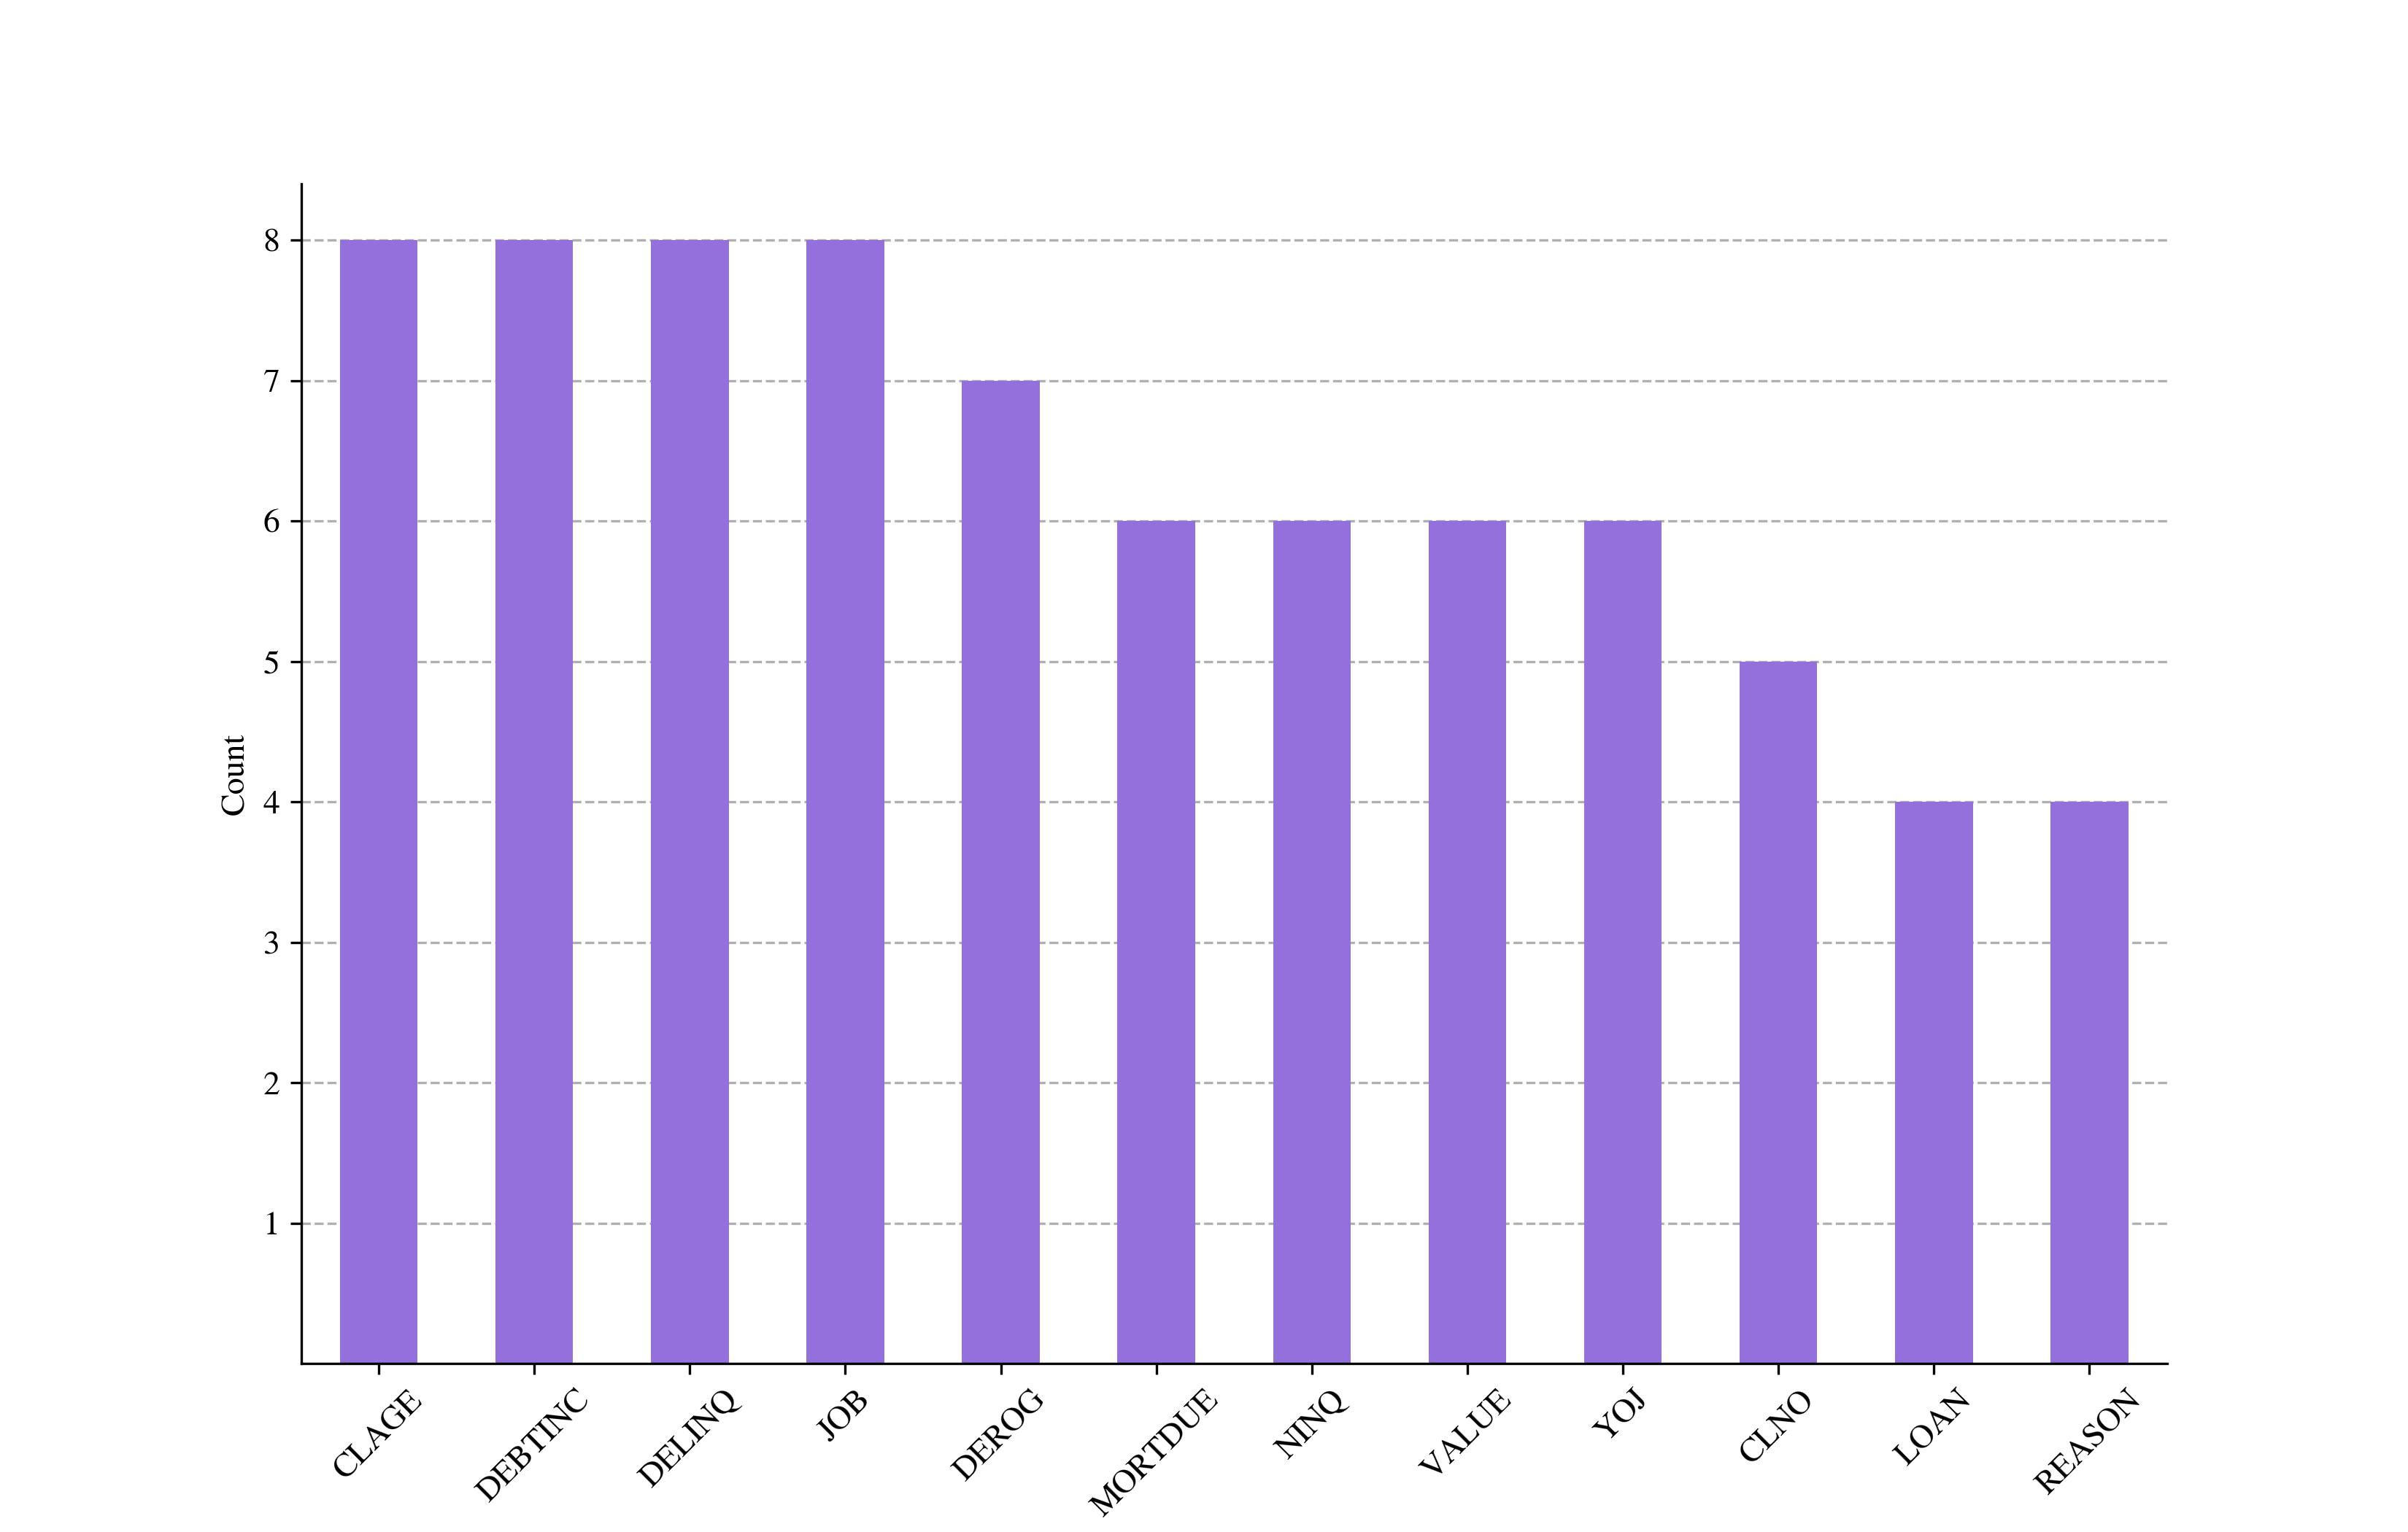
\includegraphics[width=140mm]{Figures/Recurrence_Selected_Features.jpg}
\centering{\begin{source}Author's results in Python\end{source}}\vspace{-1em}
\end{figure}


According to \autoref{fig:fsdistmod}, models such as K--Nearest Neighbors, Random Forest, Gradient Boosting and Support Vector Machine chose almost all the features as one feature feature was eliminated. On the other hand, Gaussian Naive Bayes chose only 6. It seems to be that most of the features are important as each model has selected a higher amount of features.
It is evident the more comples and/or black--box models require more features in contrast to transparant models such as Logistic Regression or Gaussian Naive Bayes.

\begin{figure}[H]
\centering
\caption{Distribution of Selected Features per Model}\vspace{0.5em}
\label{fig:fsdistmod}\
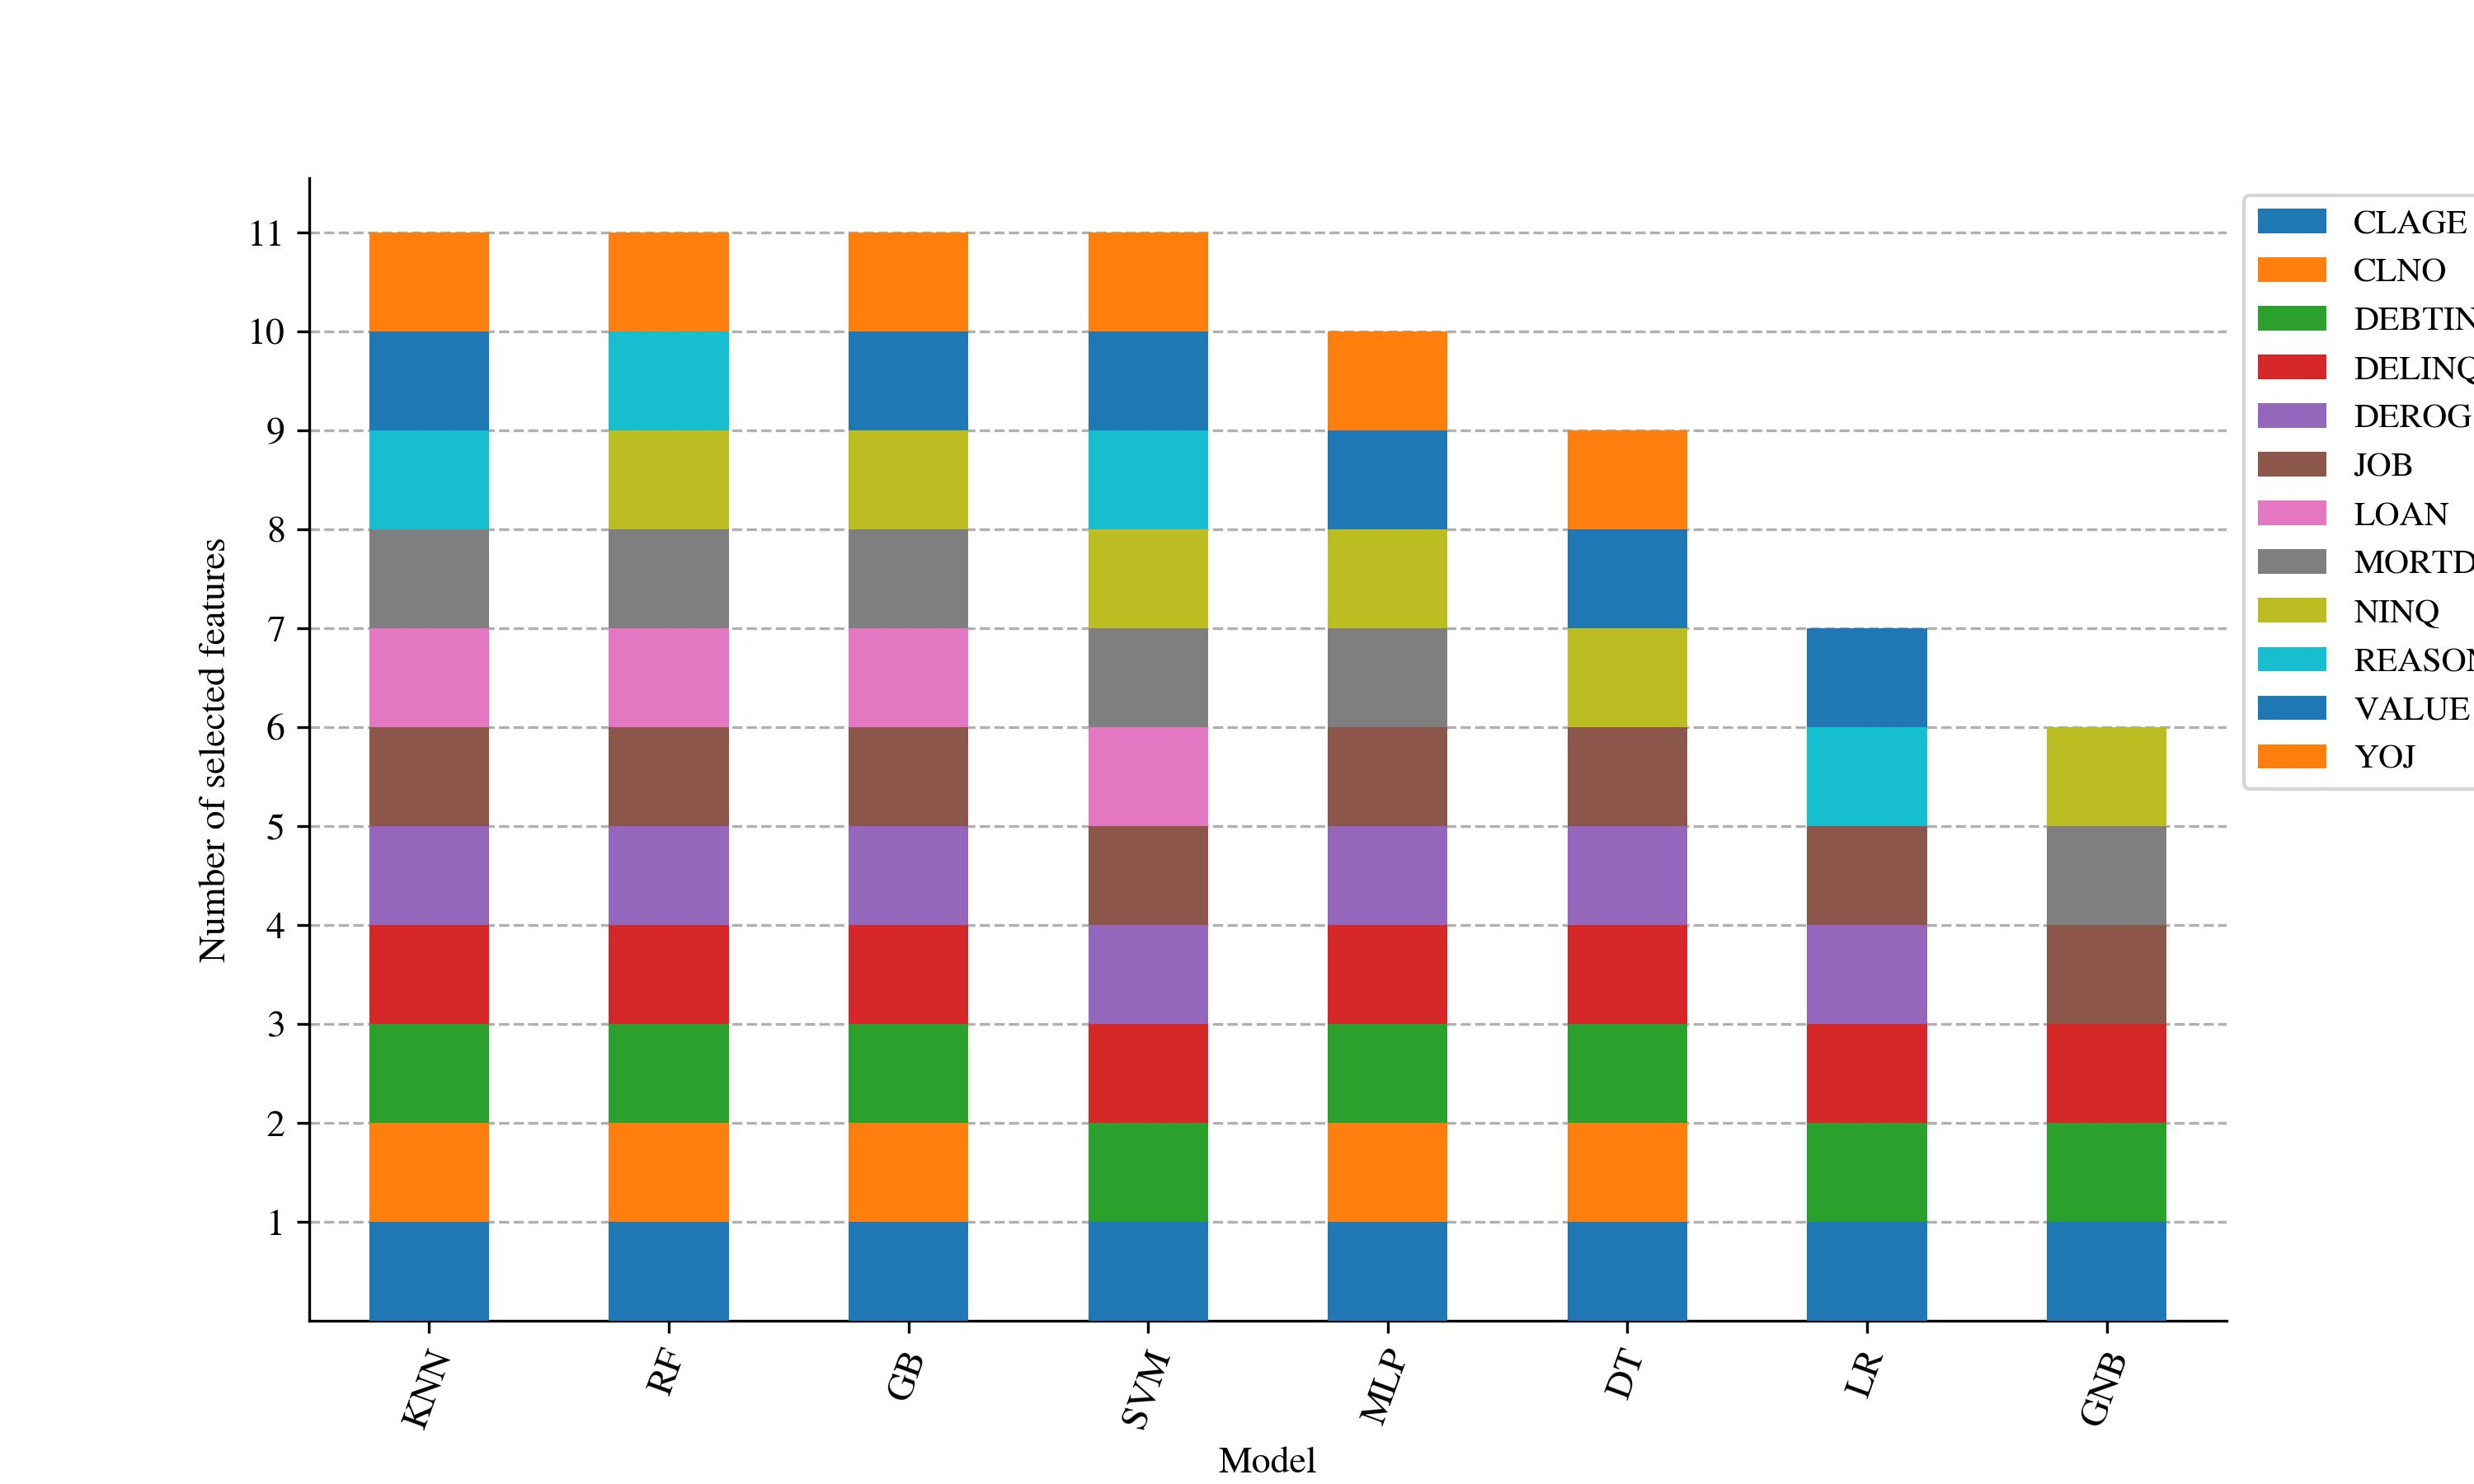
\includegraphics[width=140mm]{Figures/Selected_Features_Distribution.jpg}
\centering{\begin{source}Author's results in Python\end{source}}\vspace{-1em}
\end{figure}

\subsection{Model Selection}

In combination with the pre--selected subsets of features, the next step regards the selection of the final model. The algorithm process is described in Algorithm  \autoref{alg:model_selection} below:
\begin{algorithm}[H]
\caption{Model Selection Algorithm}
\label{alg:model_selection}
\begin{algorithmic}[1]
\For{$model \in \textit{models}$}
    \For{$F \subseteq \textit{features\_subsets}$}
        \State $\textit{optimized\_model} \gets \textsc{BayesianOptimization}(model, F)$
        \For{$\textit{metric} \in \textit{evaluation\_metrics}$}
            \State $\textit{performance} \gets \textsc{Evaluation}(\textit{optimized\_model}, \textit{metric})$
        \EndFor
    \EndFor
\EndFor
\end{algorithmic}
\end{algorithm}


\vspace{-1em}
Therefore, each input model is tuned on each subset of features selected within feature selection on the training set and subsequently, the optimized model is evaluated on the validation set. Thus, when having $n$ input models and $m$ subsets of selected features, we get $n \times m$ tuned models.
$m \leq n$ because we exclude duplicated subset of selected features which can occur when more than one model choose the same subset(s) of features.
Since there are 8 input models and 8 unique subsets of selected features, the total number of tuned models is 64.

\subsubsection{Metrics Space}

When evaluating classification models using class-based metrics such as F1 score, Precision, Recall, Accuracy, Matthews Correlation Coefficient and Jaccard Score, a default classification threshold of 0.5 is often used. This threshold separates predicted classes based on whether the predicted probability score is higher or lower than 0.5.
However, in real-world use cases, the 0.5 classification threshold may not be appropriate and according to \citep{esposito2021ghost}, such threshold is not appropriate when having imbalanced ata. Therefore, it is recommended to calculate an optimal threshold rather than relying on the default one.
For such case, the Youden index is employed which is derived from ROC curve and enables the selection of an optimal classification threshold value. 
The Younden index searches for the threshold that maximizes the sum of True Positive Rate and True Negative Rate, decreased by 1 \citep{fluss2005estimation}, thus:
\begin{equation}\label{eq}
J = TPR + TNR - 1
\end{equation}
Mathematically, the optimal threshold using Youden index is derived as follows:
\begin{equation}\label{eq}
T_{opt} = \text{argmax}_{t \in [0, 1]}\left(J\right)
\end{equation}
In Python, the \lstinline{roc_curve} function from \lstinline{Scikit-learn} returns False Positive Rate instead of the True Negative Rate. Nevertheless, we can derive the True Negative Rate from False Positive Rate as follows:
\begin{equation}\label{eq}
TNR =  1-FPR
\end{equation}
Therefore:
\begin{equation}\label{eq}
T_{opt} = \text{argmax}_{t \in [0, 1]}\left(TPR +  \left(1-FPR\right) - 1\right)
\end{equation}

In order to ensure a more comprehensive and unbiased evaluation of a model's performance, it is recommended to consider multiple metrics rather than relying on a single metric alone. This approach provides a more generalized overview of the model's performance across different aspects and helps to prevent any bias towards a single metric.
To accomplish this, models can be ranked based on their performance on each individual metric, where a higher score or a lower loss indicates a better model, resulting in a higher rank for that metric. Subsequently, for each metric, the ranking of the models is determined, and the final ranking is calculated as a weighted average of these individual rankings.
The weights have been set expertly and are summarized in \autoref{tab:weightsrank}.

Specifically, the highest weight (1.5) is assigned to the F1 score, which provides a balanced measure of a model's performance with respect to both False Positives and False Negatives.
This metric is commonly used in classification tasks, particularly in imbalanced datasets, such as the validation set in our case, which has not been oversampled.
In addition to the F1 score, higher weight is assigned to the Recall score as well (1.2), which is a metric that penalizes False Negatives.
False Negatives occur when the model predicts a negative result (i.e., no default) for an instance that is actually positive (i.e., default).
In the context of loan applications, one may prefer to reject a loan applicant who would not have defaulted (False Positive) rather than approving the application of a client who would have defaulted (False Negative). Therefore, it is appropriate to give higher weight to Recall in order to reduce the likelihood of False Negatives.
Henceforth, the weights are assigned to different metrics based on their relevance to the models' ranking, with the highest weight given to F1 score and additional weight given to Recall to ensure that False Negatives are minimized.

\begin{table}[H]
\small
\setlength{\tabcolsep}{8pt}
\renewcommand{\arraystretch}{1.3}
\centering
    \caption[Model Ranking Weights table]{Model Ranking Weights table}\label{tab:weightsrank}
    \begin{tabular}{>{\raggedleft\arraybackslash}p{0.4\linewidth} l}
\toprule
\textbf{Metric} & \textbf{Weight}\\
\midrule
\hline
F1 score & 1.5 \\
Recall & 1.2 \\
Precision & 1 \\
Accuracy & 1 \\
AUC & 1 \\
Somers' D & 1 \\ 
Kolmogorov Smirnov Distance  & 1 \\
Matthews Correlation Coefficient  & 1 \\
Jaccard Score  & 1 \\
Brier Score Loss  & 1 \\
\hline
\bottomrule
\end{tabular}
\vspace{0.7em}

\centering{\begin{source}Author's results in Python\end{source}}\vspace{-1em}
\end{table}

\subsubsection{Model Selection Results}



The custom function \lstinline{model_selection()} iteratively prints the process of the model tuning and evaluation on each subset of features, in order to keep the track of such process as it is depicted in \autoref{fig:modselprint}.
Particularly, it prints which model on which features is being tuned and evaluated, exeuction time, optimal threshold, F1 score on the validation set and the best hyperparameters.

\begin{figure}[H]
\centering\caption{Model Selection Print Statement}
\label{fig:modselprint}

{\fontsize{8.8}{11}\selectfont 
\begin{verbatim}
-------------------------------------------------------------------------------------
--------------------------------------- 56/64 ---------------------------------------
-------------------------------------------------------------------------------------
---------------------------- BAYESIAN OPTIMIZATION OF SVM ---------------------------
--------------------------- WITH FEATURES SELECTED BY MLP ---------------------------
-------------------------------------------------------------------------------------
------------------------------------------------------------------------------------- 

1/2 ... Starting Bayesian Optimization on the subset of features (10 features):
        MORTDUE, VALUE, JOB, YOJ, DEROG, DELINQ, CLAGE, NINQ, CLNO, DEBTINC
2/2... Bayesian Optimization finished 

Execution time: 22.0695 minutes 

F1 Score on Validation set: 0.7102272727272726 

Optimal classification threshold: 0.6477 

Tuned hyperparameters of SVM: 

    C: 4.999999999999999
    break_ties: False
    cache_size: 200
    class_weight: balanced
    coef0: 0.0
    decision_function_shape: ovr
    degree: 1
    gamma: scale
    kernel: rbf
    max_iter: -1
    probability: True
    random_state: 42
    shrinking: False
    tol: 1.102507160381566e-09
    verbose: False

-------------------------------------------------------------------------------------
------------------------------------------------------------------------------------- 
\end{verbatim}
}
\centering{\begin{source}Author's results in Python\end{source}}\vspace{0em}
\end{figure}



The final output of the function \lstinline{model_selection()} is table which summarizes the model's computed metrics as depicted in \autoref{tab:modelsectab}. As can be seen, the best models in terms of ranking are the Gradient Boosting models which in general have the highest score metrics and the lowest loss metrics. On the other hand, the worst-performing models are Gaussian Naive Bayes models.


\clearpage
\newpage

\KOMAoptions{paper=landscape,DIV=last}
\newgeometry{hmargin=2.5cm,bottom=25mm,height=150mm,includehead}
\fancyheadoffset{0pt}



\begin{table}[H]
\small
\setlength{\tabcolsep}{8pt}
\renewcommand{\arraystretch}{1.3}
\caption[Model Selection table]{Model Selection table}\label{tab:modelsectab}
\centering
\scalebox{0.8}{

\begin{tabular}{|p{1.3cm}|p{1.2cm}|p{1.4cm}|r|c|c|c|c|c|c|c|c|c|c|c|c|c|c|}
    \toprule
    \textbf{Tuned model} & \textbf{FS model} & \# \newline Features & Time & Thres & F1 & Prec & Rec & Acc & AUC & SD & KS & MCC & JC & BSL & Log Loss & rank \\
    \midrule
    \hline
    GB & MLP & 10 & 12.30 & 0.4955 & 0.7809 & 0.7853 & 0.7765 & 0.9128 & 0.9515 & 0.9030 & 0.7751 & 0.7265 & 0.6406 & 0.0666 & 0.2487 & 1 \\
GB & KNN & 11 & 12.80 & 0.5072 & 0.7978 & 0.7912 & 0.8045 & 0.9184 & 0.9587 & 0.9175 & 0.7989 & 0.7467 & 0.6636 & 0.0687  & 0.4135 & 2 \\
GB & SVM & 11 & 15.08 & 0.5053 & 0.7896 & 0.8155 & 0.7654 & 0.9184 & 0.9555 & 0.9109 & 0.7961 & 0.7397 & 0.6524 & 0.0718  & 0.3486 & 3 \\
GB & GB & 11 & 11.44 & 0.4132 & 0.7799 & 0.7778 & 0.7821 & 0.9117 & 0.9543 & 0.9086 & 0.7989 & 0.7247 & 0.6393 & 0.0703  & 0.3372 & 4 \\
GB & RF & 11 & 13.38 & 0.4973 & 0.7775 & 0.7841 & 0.7709 & 0.9117 & 0.9541 & 0.9081 & 0.7961 & 0.7225 & 0.6359 & 0.0669 & 0.2803 & 5 \\
RF & KNN & 11 & 5.94 & 0.4725 & 0.7486 & 0.7326 & 0.7654 & 0.8972 & 0.9226 & 0.8452 & 0.7109 & 0.6843 & 0.5983 & 0.0923 & 0.3232 & 6 \\
GB & DT & 9 & 12.00 & 0.4729 & 0.7675 & 0.7697 & 0.7654 & 0.9073 & 0.9407 & 0.8814 & 0.7556 & 0.7096 & 0.6227 &0.0808 &  0.4693 & 7 \\
RF & GB & 11 & 5.18 & 0.4517 & 0.7385 & 0.7135 & 0.7654 & 0.8916 & 0.9200 & 0.8400 & 0.7123 & 0.6709 & 0.5855 & 0.0886  & 0.3135 & 8 \\
RF & MLP & 10 & 6.62 & 0.4761 & 0.7357 & 0.7181 & 0.7542 & 0.8916 & 0.9179 & 0.8358 & 0.7081 & 0.6679 & 0.5819 & 0.0879  & 0.3084 & 9 \\
GB & LR & 7 & 16.81 & 0.4362 & 0.7388 & 0.7000 & 0.7821 & 0.8894 & 0.9219 & 0.8438 & 0.7081 & 0.6706 & 0.5858 & 0.0886 & 0.3925 & 10 \\
\ldots & \ldots & \ldots & \ldots & \ldots & \ldots & \ldots & \ldots & \ldots & \ldots & \ldots & \ldots & \ldots & \ldots & \ldots & \ldots & \ldots \\
GNB & LR & 7 & 0.39 & 0.2990 & 0.6099 & 0.5094 & 0.7598 & 0.8056 & 0.8420 & 0.6840 & 0.5866 & 0.5043 & 0.4387 & 0.1340 & 0.6458
& 55 \\
DT & GNB & 6 & 0.89 & 0.5000 & 0.6354 & 0.6284 & 0.6425 & 0.8525 & 0.8187 & 0.6375 & 0.5838 & 0.5430 & 0.4656 & 0.1251 &  2.1679 & 56 \\
GNB & KNN & 11 & 0.38 & 0.3588 & 0.6093 & 0.5219 & 0.7318 & 0.8123 & 0.8479 & 0.6957 & 0.5698 & 0.5024 & 0.4381 & 0.1367  & 0.6686 & 57 \\
GNB & DT & 9 & 0.39 & 0.2241 & 0.6063 & 0.5095 & 0.7486 & 0.8056 & 0.8467 & 0.6935 & 0.5768 & 0.4991 & 0.4351 & 0.1316 &  0.6370 & 58 \\
GNB & GB & 11 & 0.38 & 0.1829 & 0.5969 & 0.4893 & 0.7654 & 0.7933 & 0.8531 & 0.7063 & 0.5810 & 0.4880 & 0.4255 & 0.1310  & 0.6461 & 59 \\
GNB & MLP & 10 & 0.39 & 0.2194 & 0.6013 & 0.5000 & 0.7542 & 0.8000 & 0.8493 & 0.6986 & 0.5768 & 0.4930 & 0.4299 & 0.1319  & 0.6360 & 60 \\
GNB & GNB & 6 & 0.38 & 0.4787 & 0.5950 & 0.5039 & 0.7263& 0.8022 & 0.8356 & 0.6711 & 0.5559 & 0.4835 & 0.4235 & 0.1470 &  0.5280 & 61 \\
LR & GNB & 6 & 1.59 & 0.4561 & 0.5948 & 0.5121 & 0.7095 & 0.8067 & 0.8379 & 0.6758 & 0.5531 & 0.4831 & 0.4233 & 0.1319  & 0.4180 & 62 \\
GNB & SVM & 11 & 0.38 & 0.1991 & 0.5885 & 0.4872 & 0.7430 & 0.7922 & 0.8425 & 0.6850 & 0.5712 & 0.4756 & 0.4169 & 0.1345  & 0.6721 & 63 \\
GNB & RF & 11 & 0.39 & 0.3413 & 0.5864 & 0.4943 & 0.7207 & 0.7966 & 0.8288 & 0.6577 & 0.5545 & 0.4720 & 0.4148 & 0.1486 &  0.7040 & 64 \\
    \hline
    \bottomrule 
\end{tabular}}
\vspace{1em}

\centering{\begin{source}Author's results in Python\end{source}}\vspace{-1em}
\end{table}

\clearpage
\newpage
\KOMAoptions{paper=portrait,DIV=last}
\restoregeometry
\fancyheadoffset{0pt}

In order to gain a more detailed understanding of the model selection results, the distribution of computed metrics is plotted. In \autoref{fig:f1dist}, the F1 score distribution is visualized for each input model. An outlier can be observed in KNN where the F1 score is 0.				
\begin{figure}[H]
\centering
\caption{F1 score distribution}\vspace{0.5em}
\label{fig:f1dist}\
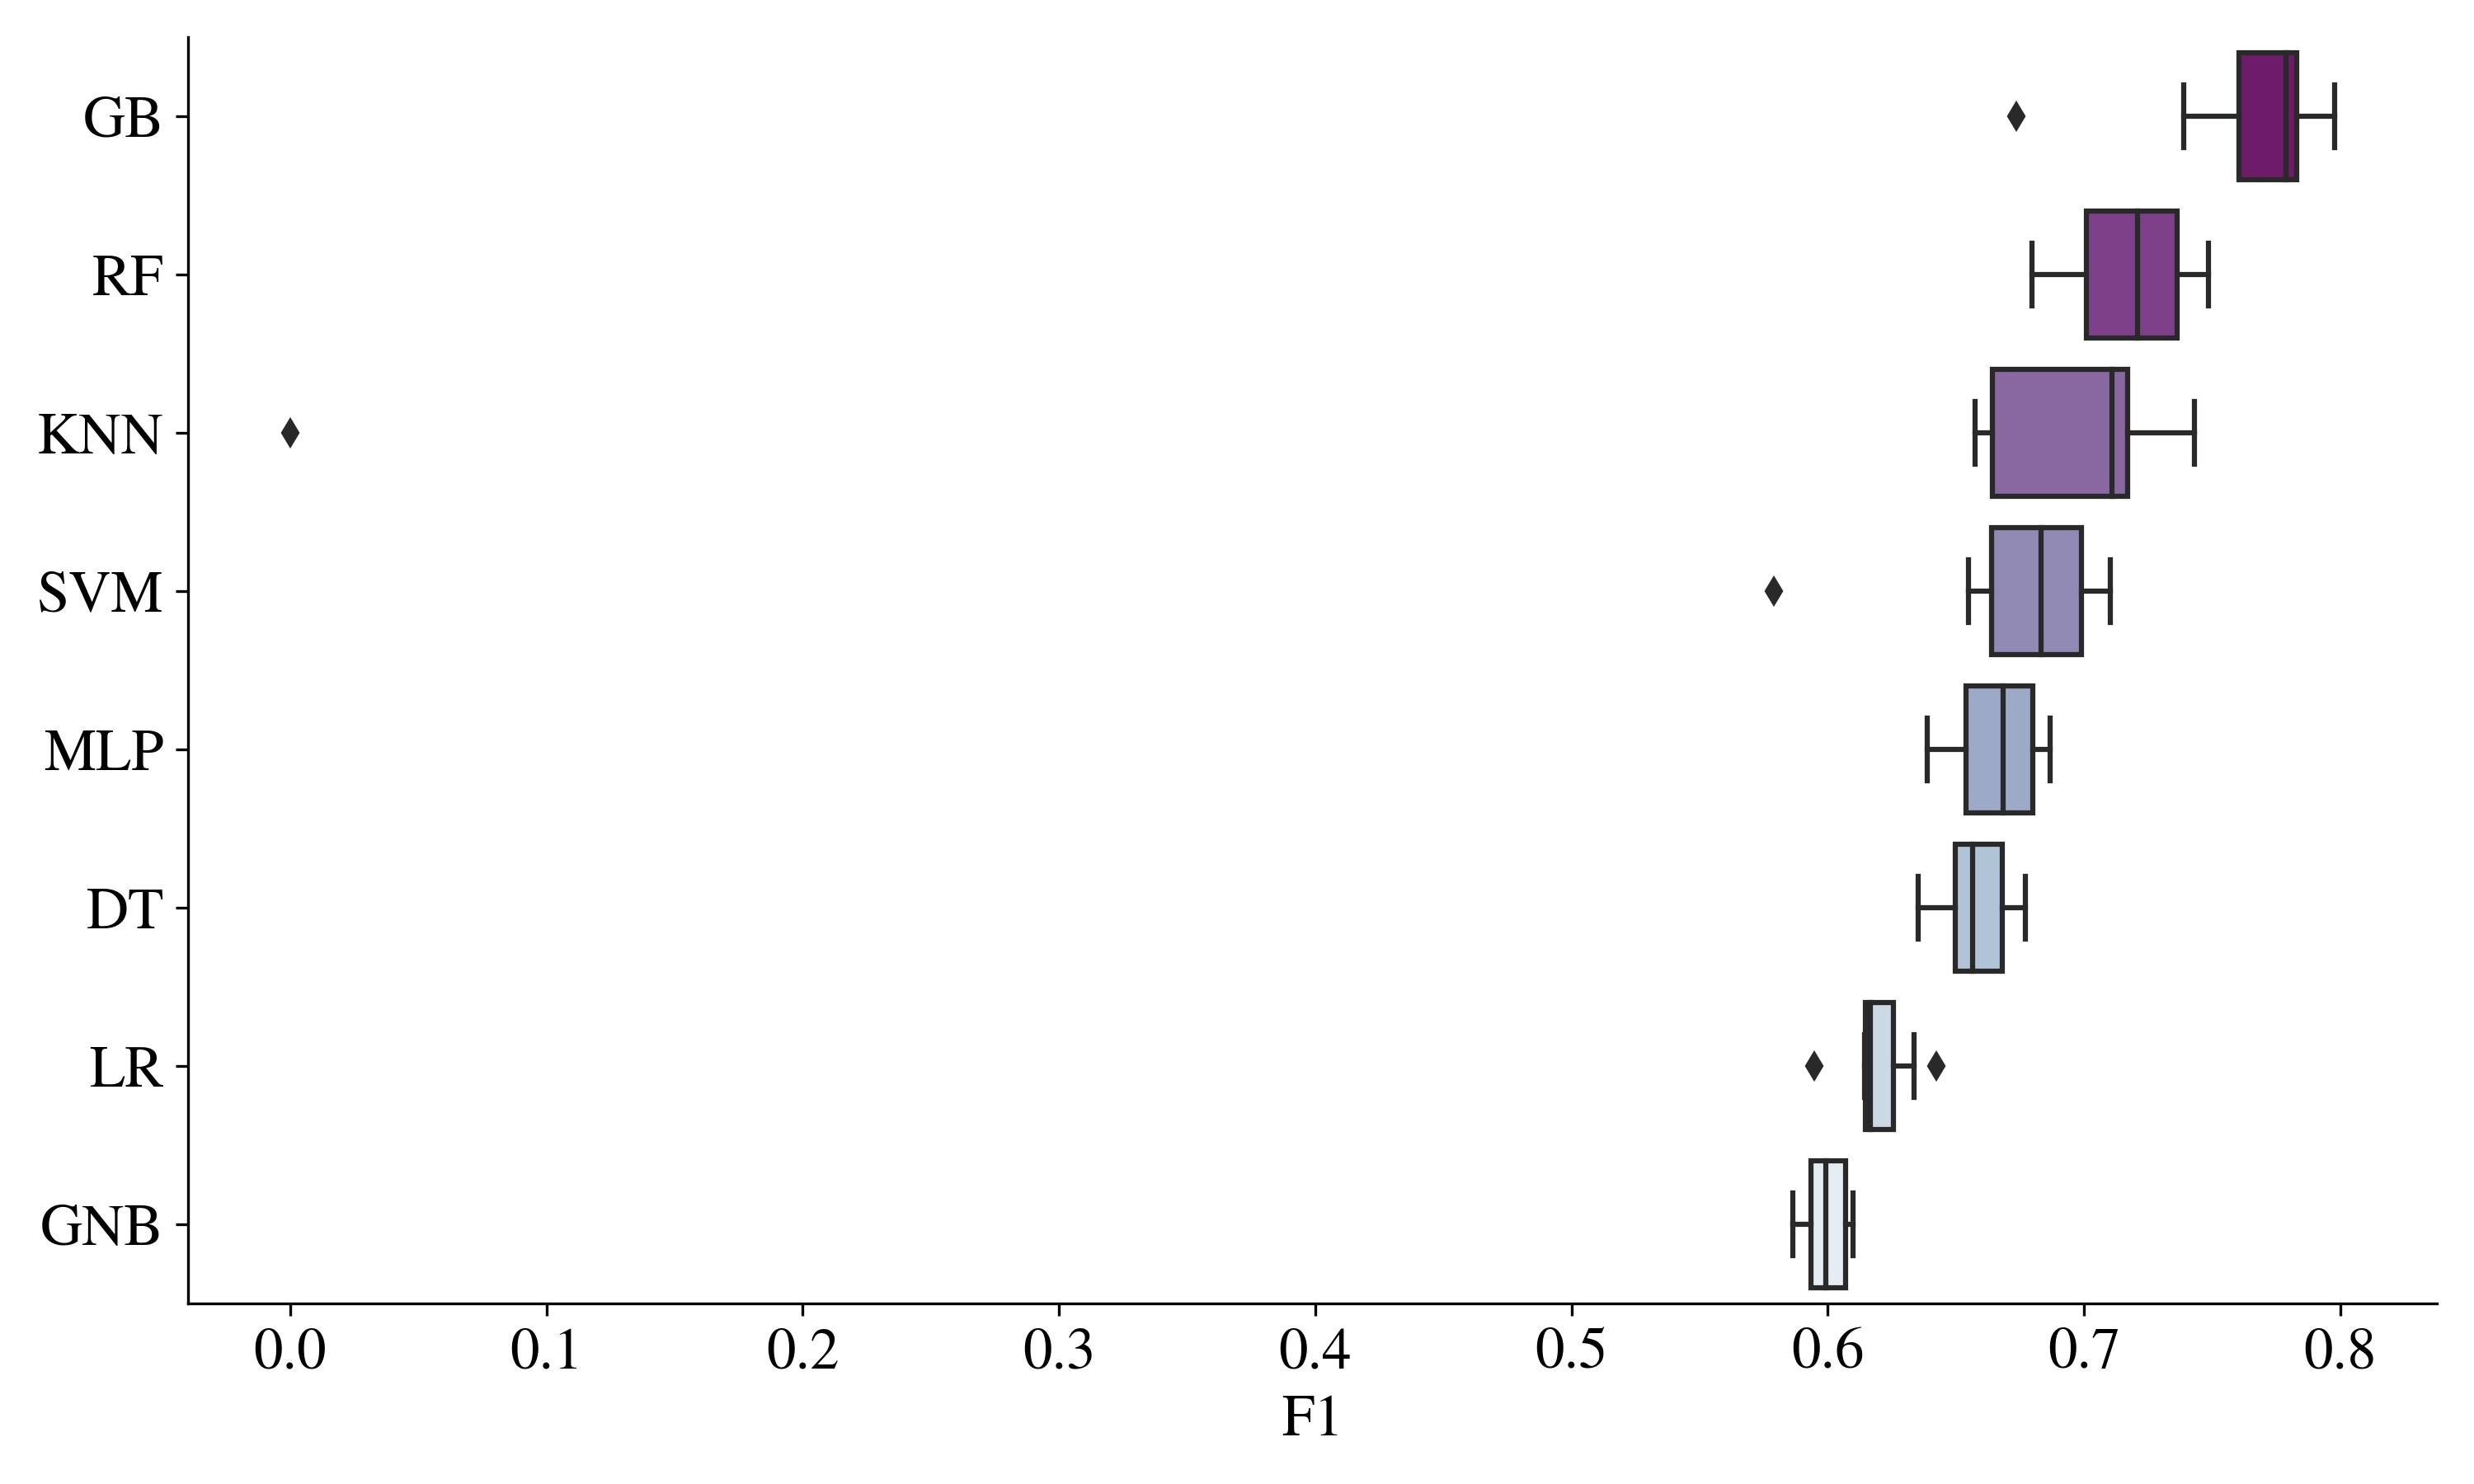
\includegraphics[width=140mm]{Figures/F1_Distribution.jpg}
\centering{\begin{source}Author's results in Python\end{source}}\vspace{-1em}
\end{figure}
Such outlier is removed in \autoref{fig:f1distclean} to gain a more general insight into the F1 score distribution.
It can be observed that Gradient Boosting models have the highest F1 scores of around 80 \%.
Another tree ensemble model, Random Forest, is performing well as the second best. However, more transparent models such as Logistic Regression and Naive Bayes are performing poorly, having F1 scores around 60 \%.
Surprisingly, black box models such as Support Vector Machine and Neural Network are outperformed by the less complex KNN model.
Nonetheless, given the relatively small sample size, KNN performs better than Neural Network and non-linear SVM on small datasets, whereas NN or non-linear SVM generally outperform KNN when it comes to large datasets.
\begin{figure}[H]
\centering
\caption{F1 score distribution - without outliers}\vspace{0.5em}
\label{fig:f1distclean}\
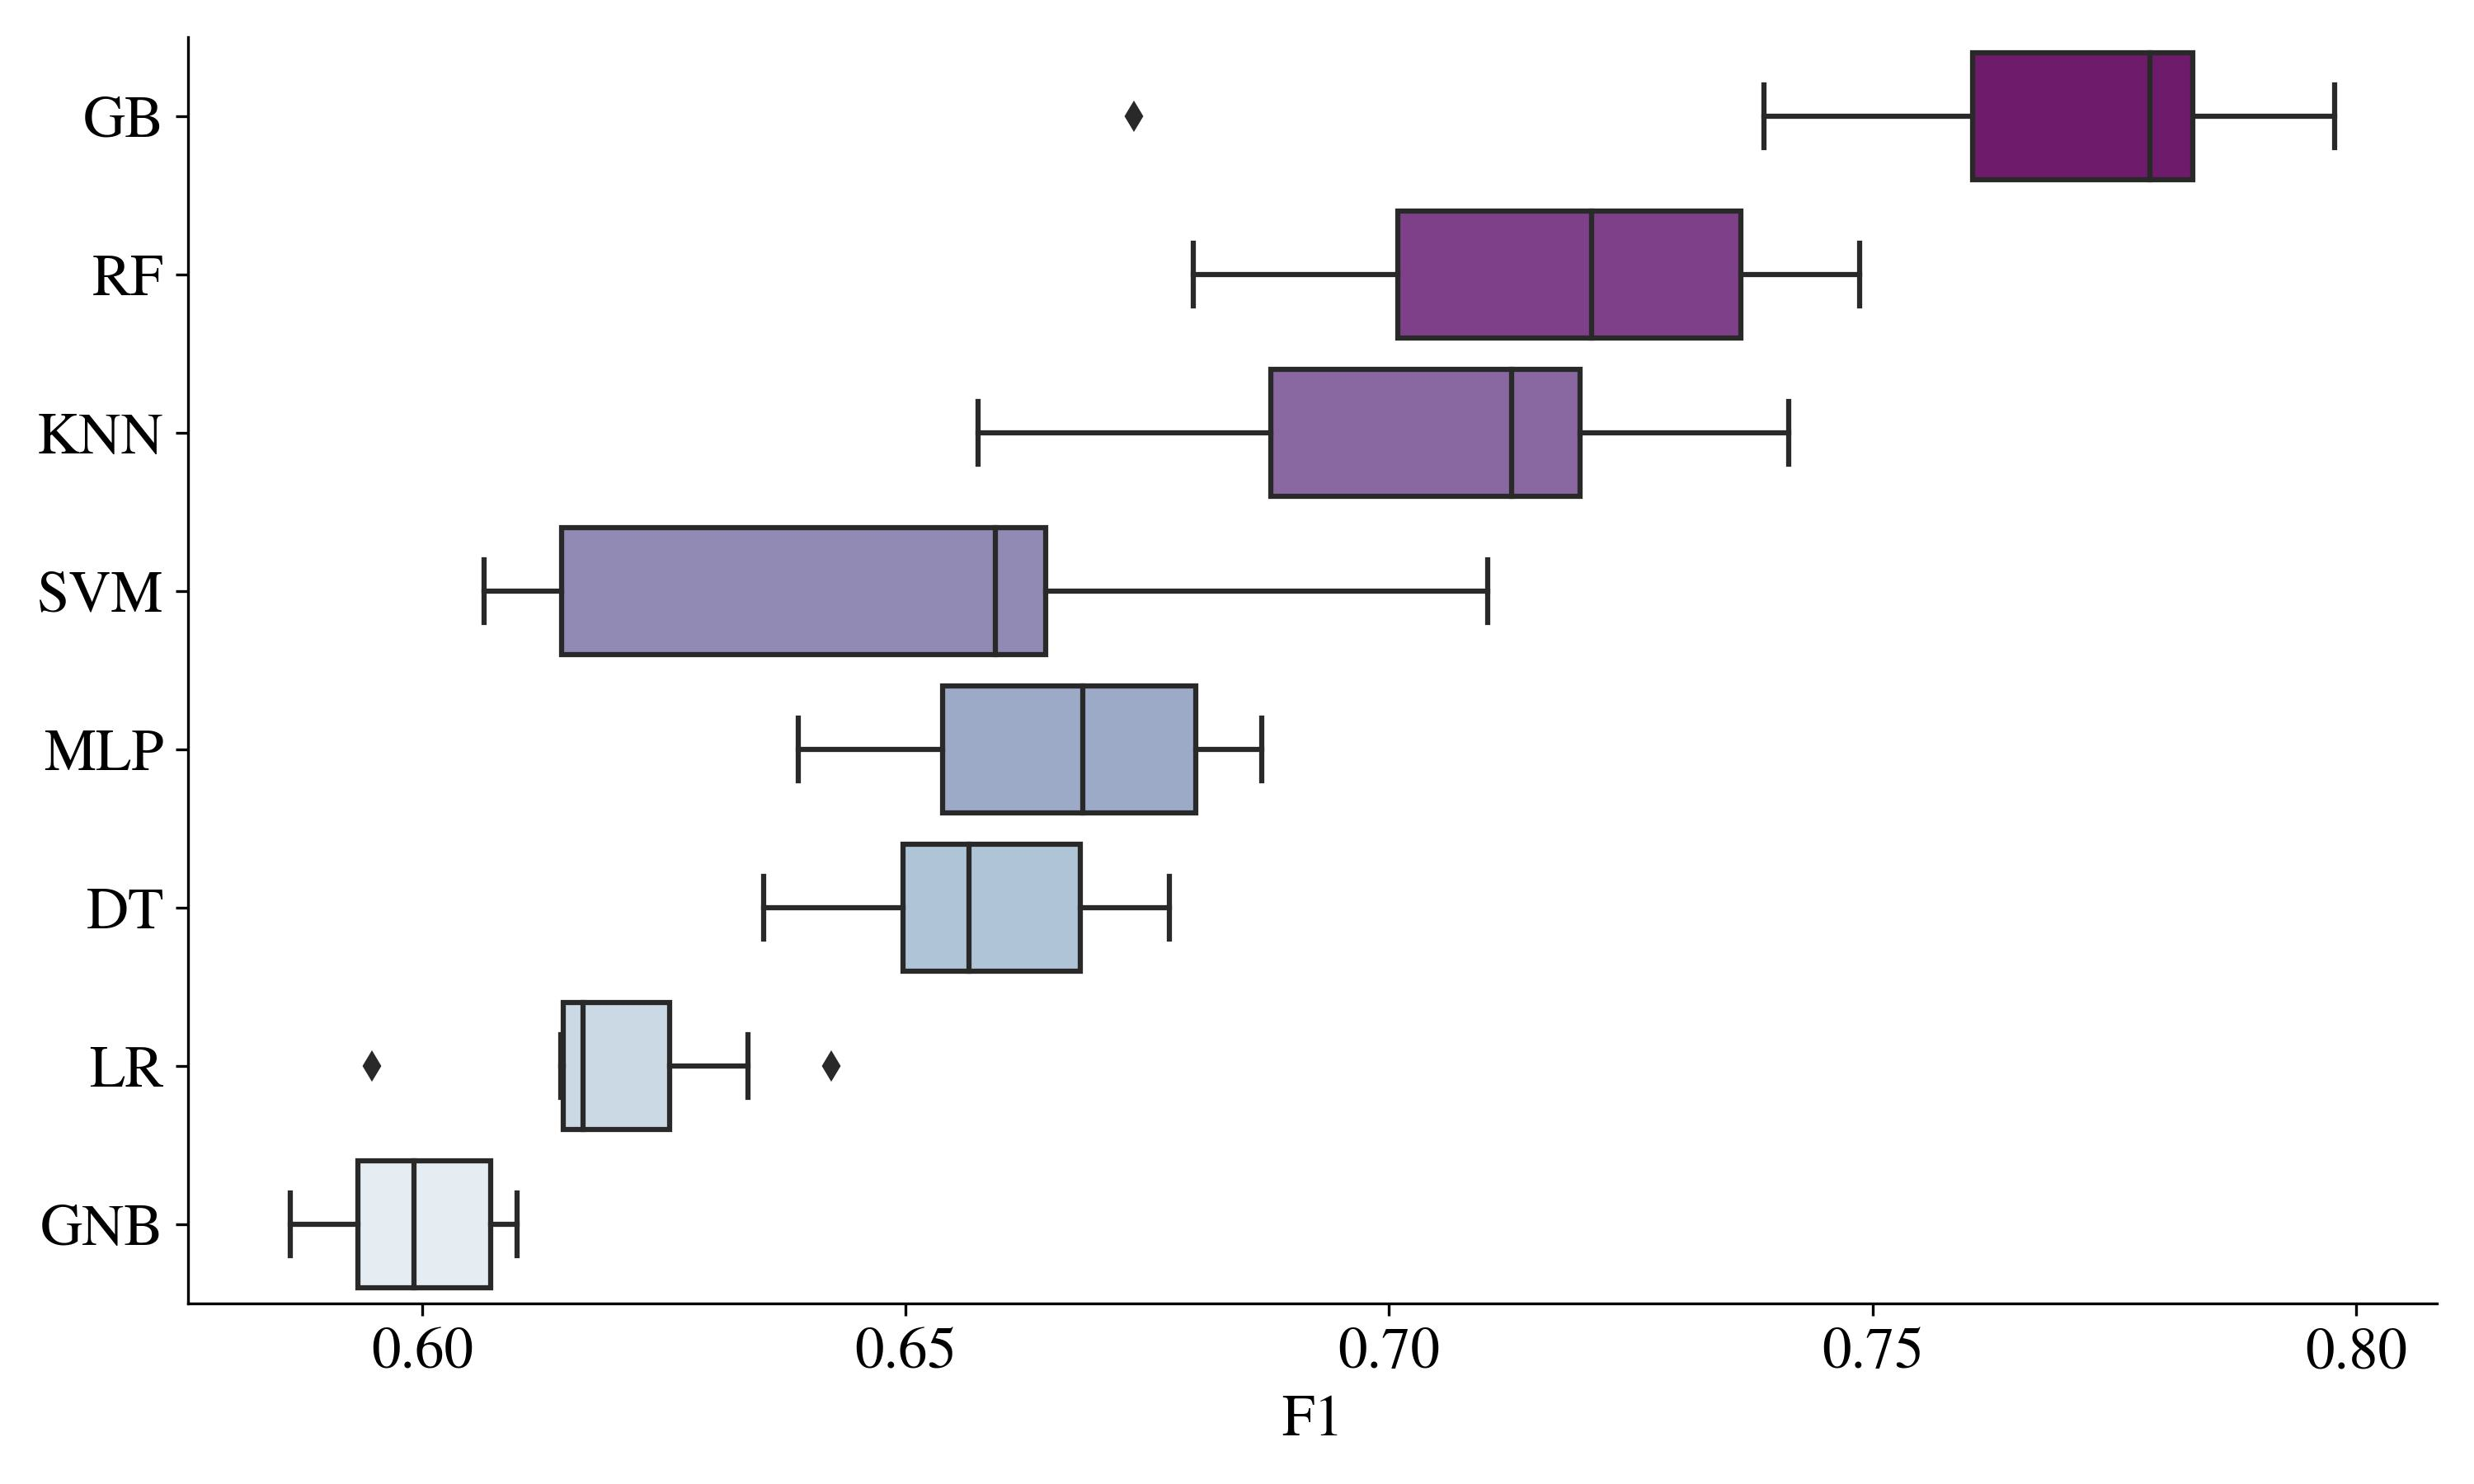
\includegraphics[width=140mm]{Figures/F1_wo_outliers_Distribution.jpg}
\centering{\begin{source}Author's results in Python\end{source}}\vspace{-1em}
\end{figure}

The optimal threshold distribution for each base model is presented in \autoref{fig:thresdist}. We can observe an outlier in KNN having a threshold value of 1, which explains the F1 score outlier found previously in \autoref{fig:f1dist}.
\begin{figure}[H]
\centering
\caption{Threshold distribution}\vspace{0.5em}
\label{fig:thresdist}\
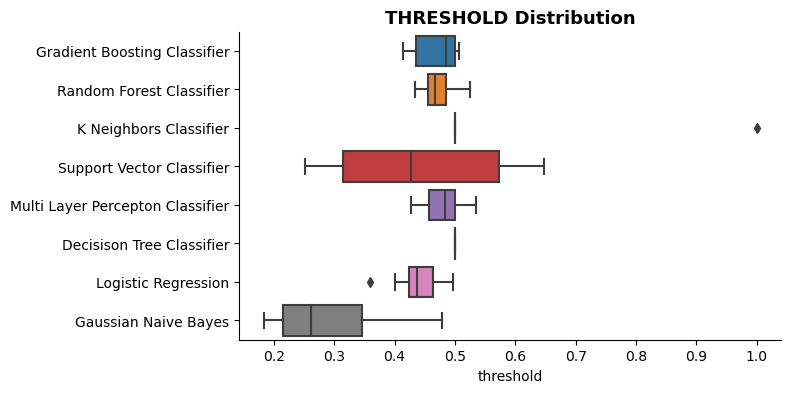
\includegraphics[width=140mm]{Figures/Threshold_Distribution.jpg}
\centering{\begin{source}Author's results in Python\end{source}}\vspace{-1em}
\end{figure}

In order to obtain a better insight into the distribution of optimal thresholds, the outlier in KNN is excluded, resulting in the threshold distribution depicted in \autoref{fig:thresdistclean}. The optimal threshold values are mostly distributed below 0.5, indicating that the models are generally more conservative. The most conservative model is Gaussian Naive Bayes, which has a median threshold value around 0.25.
\begin{figure}[H]
\centering
\caption{Threshold distribution - without outliers}\vspace{0.5em}
\label{fig:thresdistclean}\
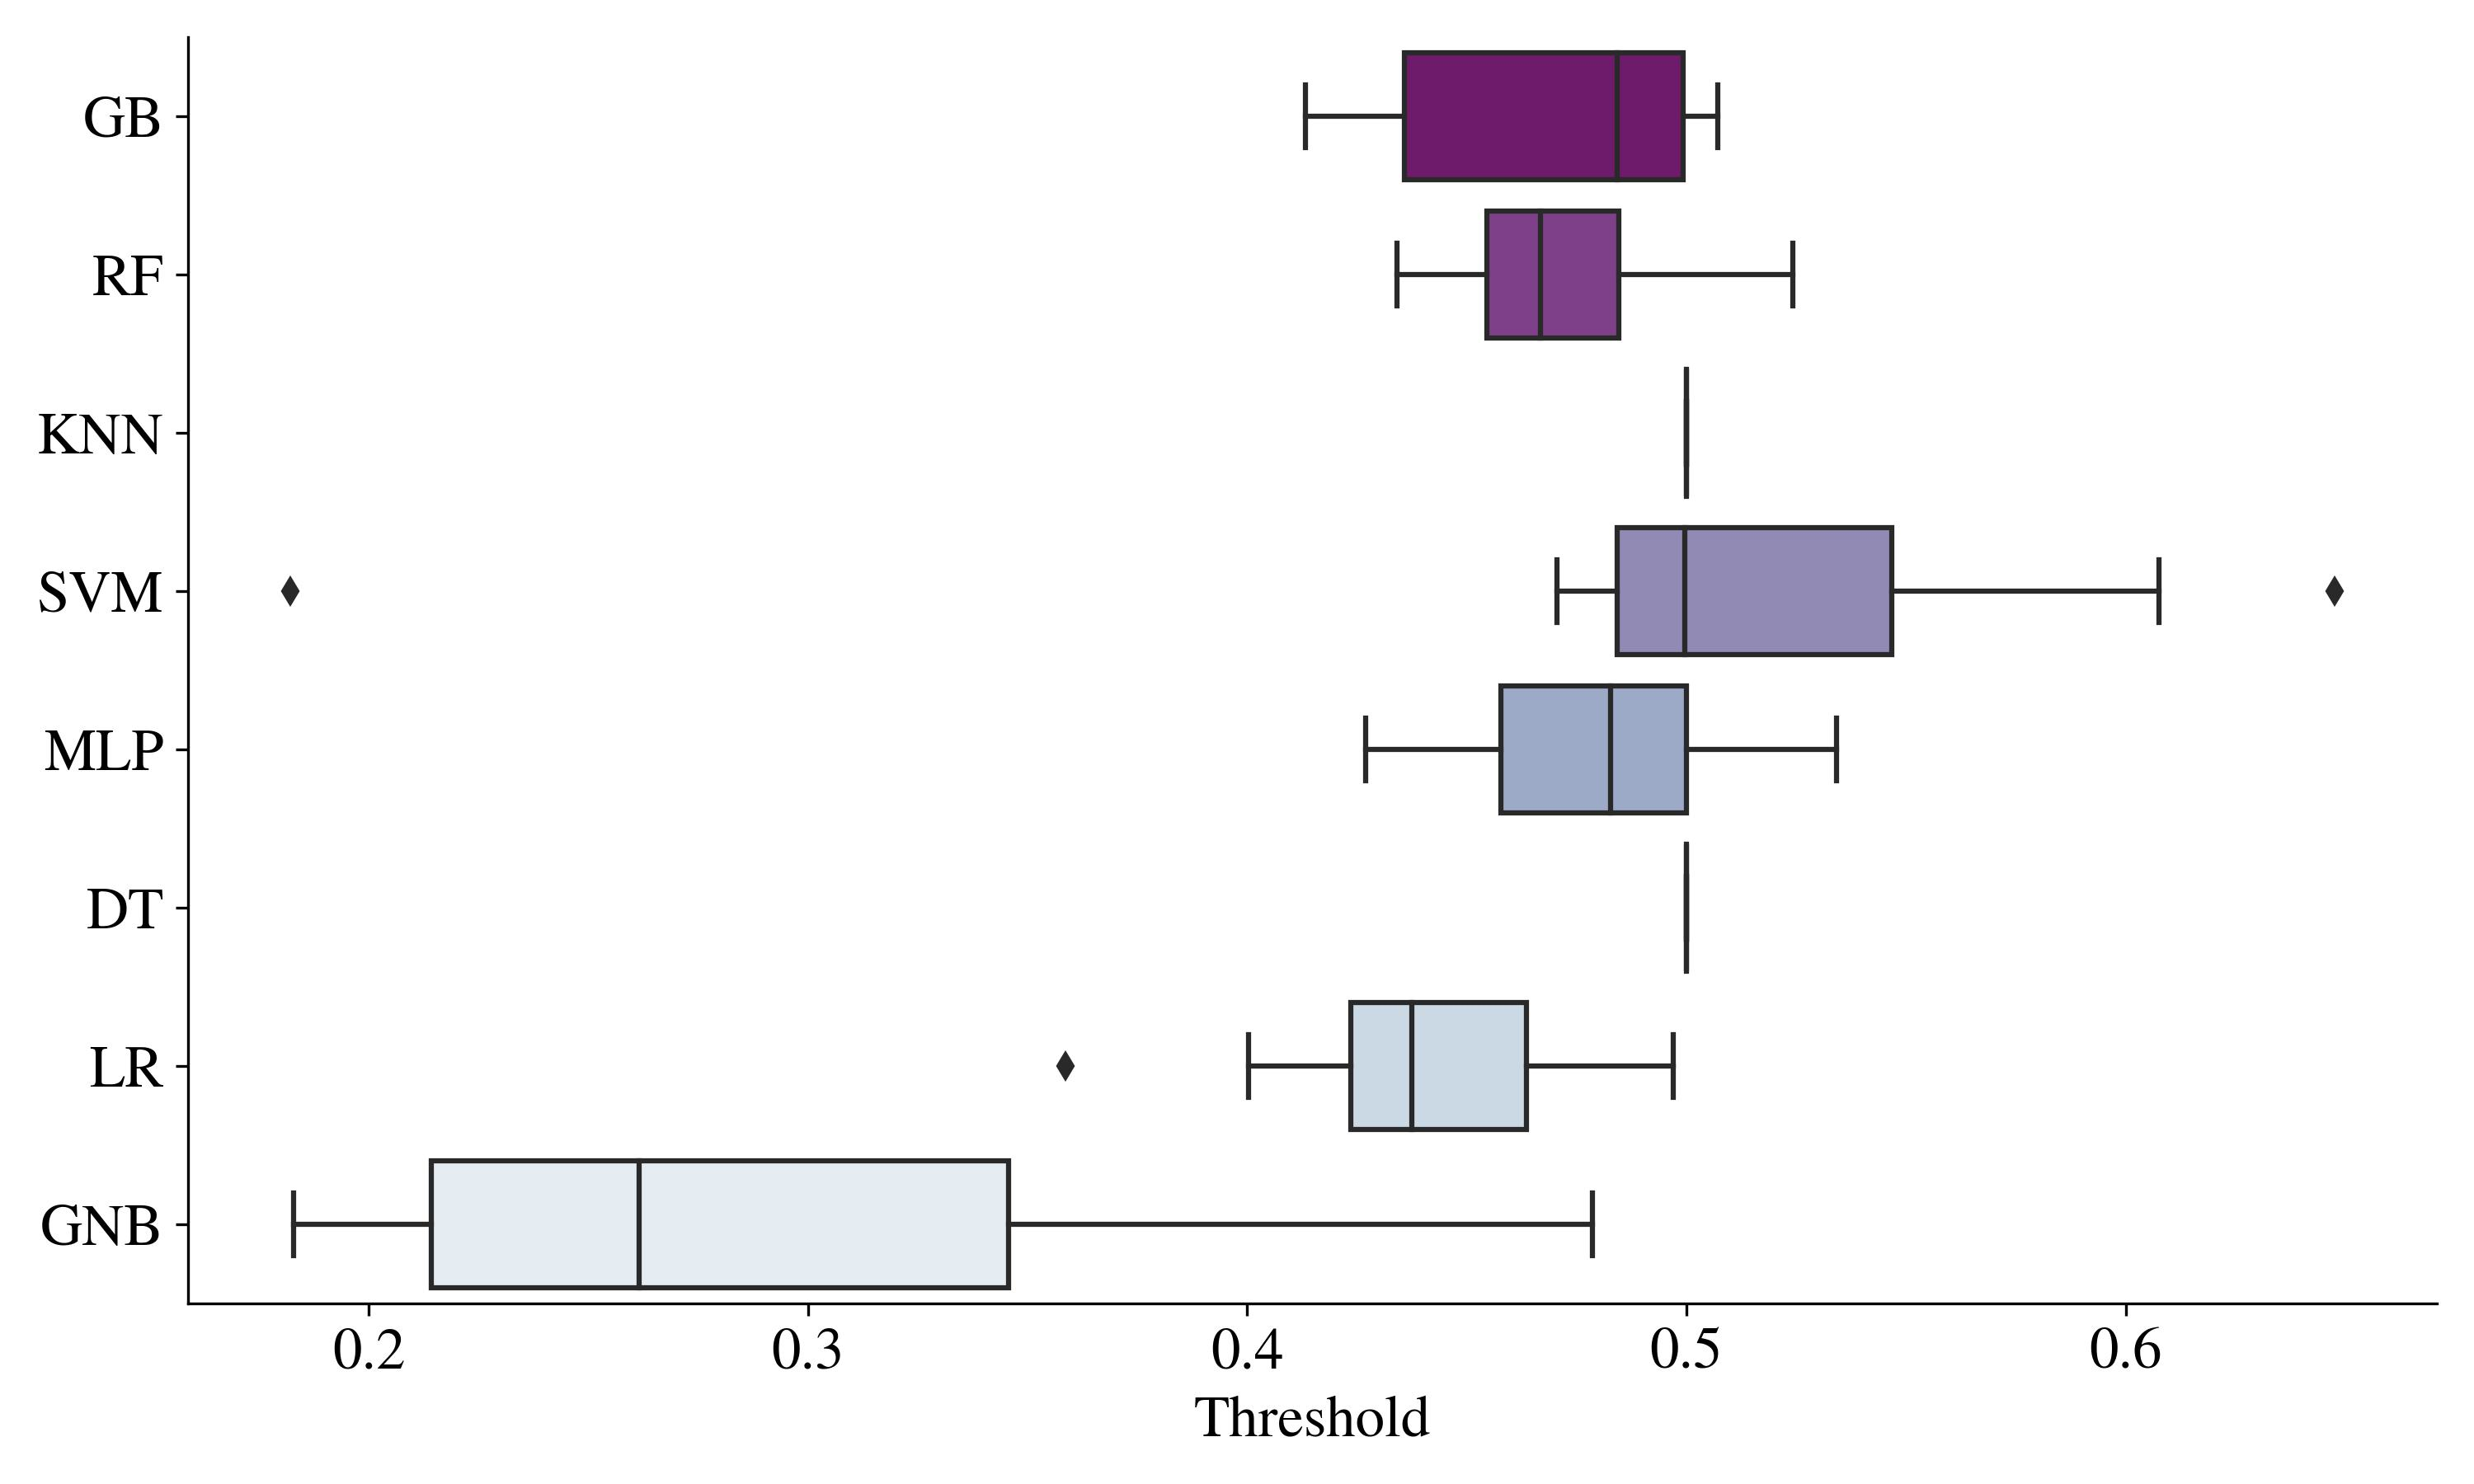
\includegraphics[width=140mm]{Figures/Threshold_wo_outliers_Distribution.jpg}
\centering{\begin{source}Author's results in Python\end{source}}\vspace{-1em}
\end{figure}

Upon examining the optimization time of each model, it can be observed that the transparent and non-complex models such as Logistic Regression, Gaussian Naive Bayes, or even Decision Tree, which take around only 1 minute to optimize themselves, also perform poorly, as already inspected in \autoref{fig:f1distclean}.
Conversely, the most time-consuming models are undoubtedly the Neural Network models, which take around 30 minutes to optimize themselves. Other time-consuming models include Gradient Boosting and Support Vector Machine, which take around 13 and 11 minutes to optimize themselves, respectively.
This finding suggests that longer optimization time does not necessarily lead to better performance, as the Neural Network models are significantly outperformed by several other models.
\begin{figure}[H]
\centering
\caption{Execution time distribution}\vspace{0.5em}
\label{fig:timedist}\
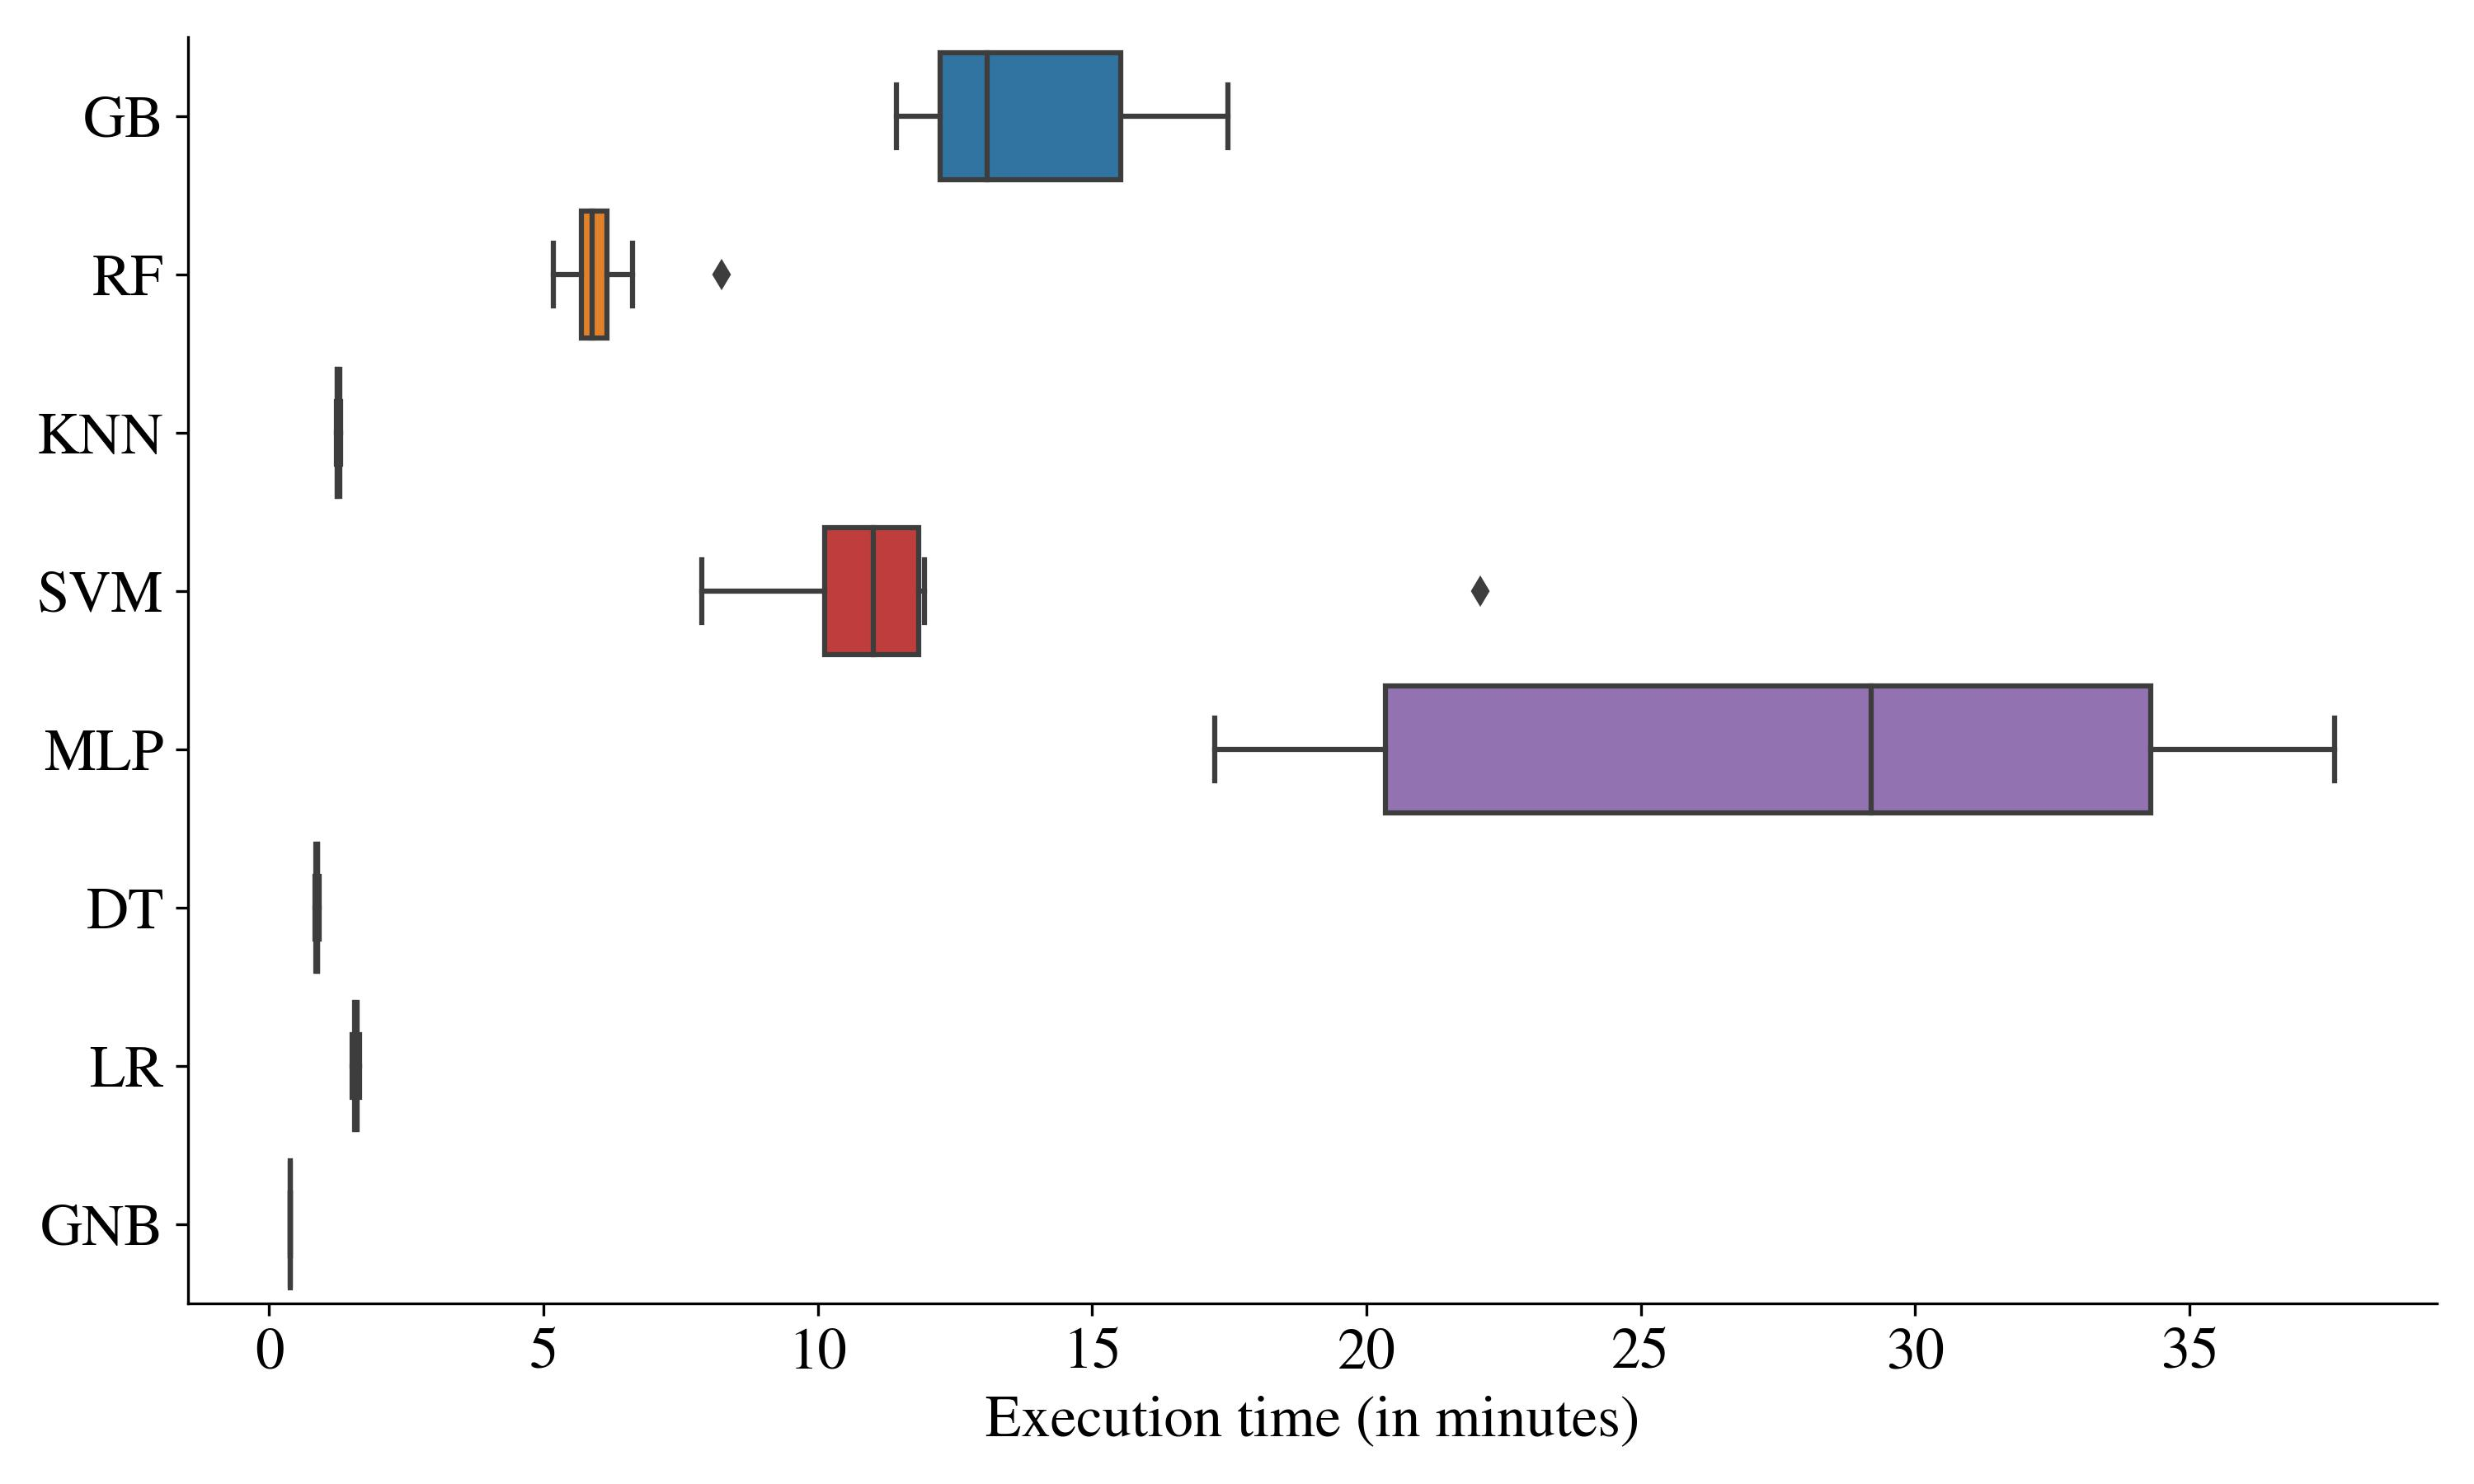
\includegraphics[width=140mm]{Figures/EXECUTION_TIME_Distribution.jpg}
\centering{\begin{source}Author's results in Python\end{source}}\vspace{-1em}
\end{figure}

The execution time and the F1 score were inspected together using a scatterplot, as shown in \autoref{fig:scattertime}.
A cluster of non-complex and transparent models, such as Logistic Regression, Gaussian Naive Bayes, Decision Tree, and KNN, can be observed around the vertical line near 0 execution time. These models are quick to optimize, but their F1 scores are generally low, except for KNN.
Further, their variance in execution time is quite low, regardless of the feature subset they are optimized on.
On the other hand, the Neural Network models always perform poorly, regardless of the length of the execution time. Furthermore, the variance of the F1 scores is quite low for these models, indicating that the execution time does not have a significant impact on the F1 score in the case of Neural Networks.

\begin{figure}[H]
\centering
\caption{Execution time vs. F1 Scatterplot}\vspace{0.5em}
\label{fig:scattertime}\
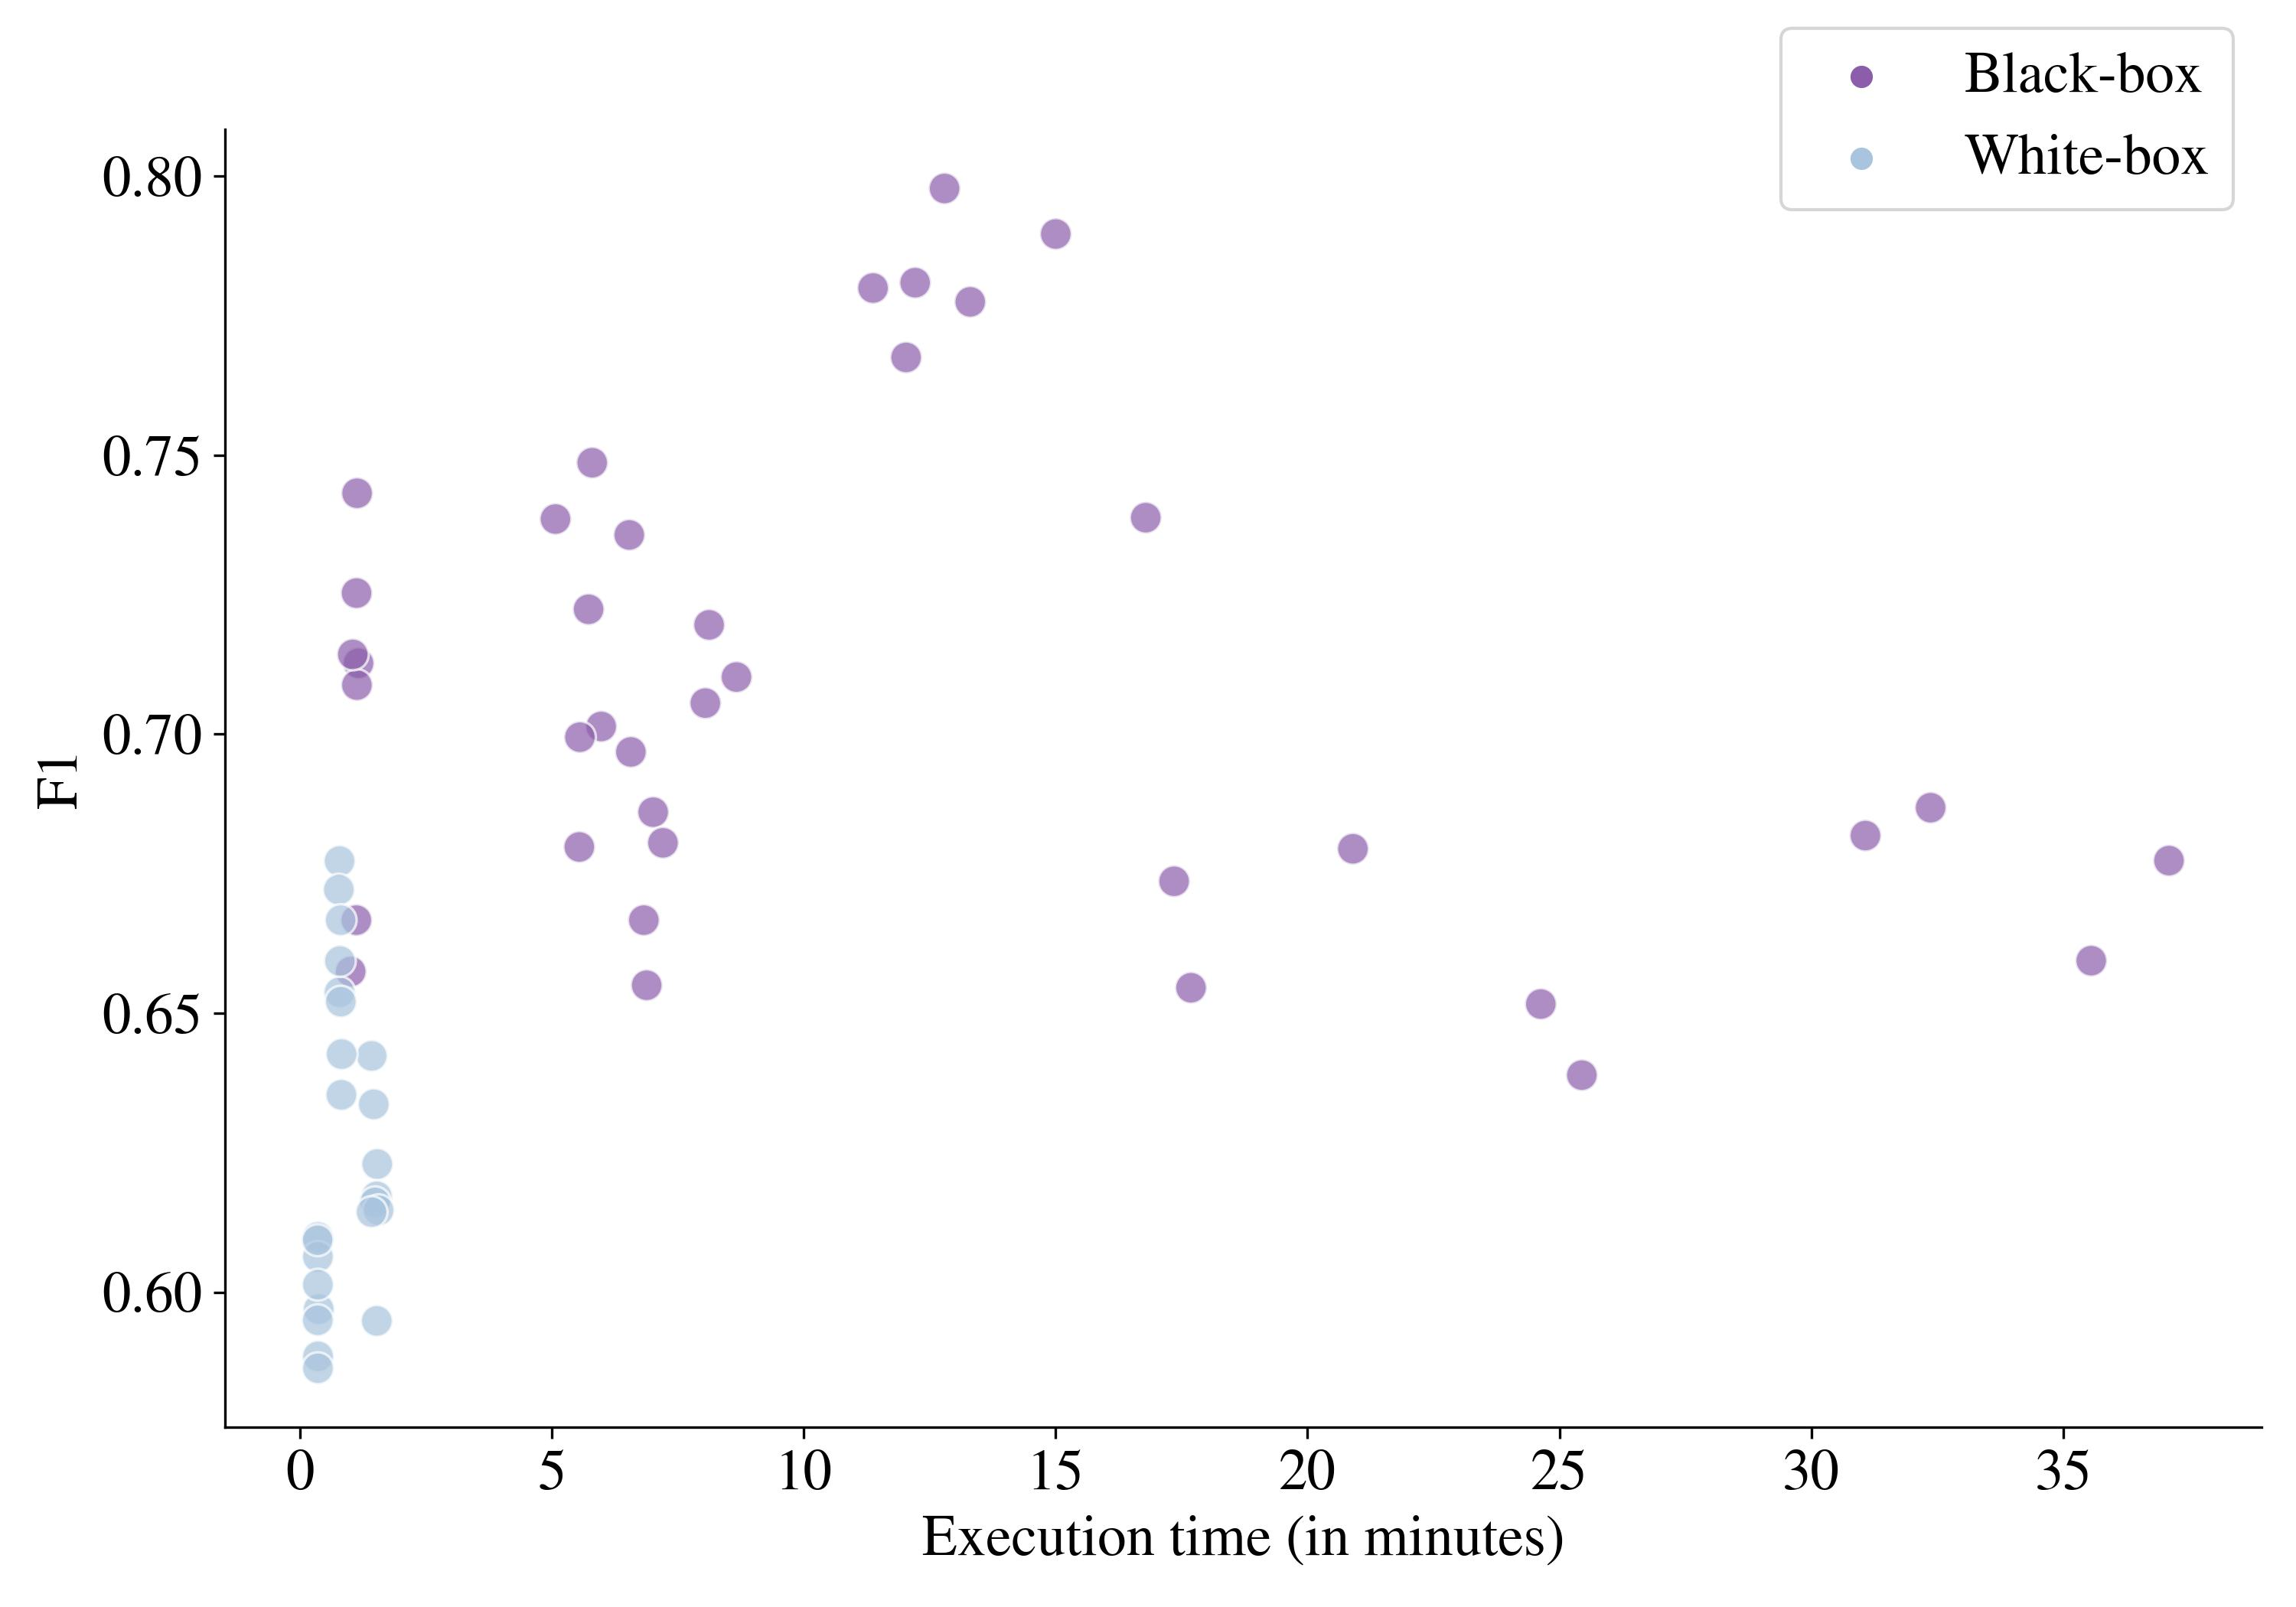
\includegraphics[width=140mm]{Figures/Scatterplot_execution_time_F1_wo_outliers.jpg}
\centering{\begin{source}Author's results in Python\end{source}}\vspace{-1em}
\end{figure}

To summarize this subsection, the best and final model is the Gradient Boosting Classifier which was optimized on the subset of features selected by Multi-Layer Percepton - both the model information and its final hyperparameters' values are described in \autoref{tab:finalmodelinfo}. Such model is then used in the next modelling steps, including the recalibration, evaluation and deployment.
\begin{table}[H]
    \small
    \setlength{\tabcolsep}{8pt}
    \renewcommand{\arraystretch}{1.3}
    \centering
    \caption{Final Model Information}\label{tab:finalmodelinfo}
    \begin{tabular}{>{\raggedleft\arraybackslash}p{0.20\linewidth}|p{0.65\linewidth}}
    \toprule
    \midrule
    \textbf{Final Model} & Gradient Boosting \\
    \midrule
    \textbf{FS Model} & Multi--Layer Percepton \\
    \midrule
    \textbf{Final Features} &
    MORTDUE, VALUE, JOB, YOJ, DEROG, DELINQ, CLAGE, NINQ, CLNO, DEBTINC \\
    \midrule
    \textbf{Threshold} & 0.4955 \\
    \midrule
    \textbf{F1} & 0.7809 \\
    \midrule
    \textit{\# estimators} & 1,000 \\
    \midrule
    \textit{Criterion} & Friedman MSE \\
    \midrule
    \textit{Max depth} & 10 \\
    \midrule
    \textit{Max features} & 1 \\
    \midrule
    \textit{Loss} & Log loss \\
    \midrule
    \textit{Learning rate} & 0.0150 \\
    \midrule
    \bottomrule
    \end{tabular}
    \vspace{0.5em}
    
    \centering{\begin{source}Author's results in Python\end{source}}\vspace{-0.5em}
\end{table}

\subsection{Model Recalibration}

In order to ensure that the final model performs well on unseen data, it is common practice to employ the recalibration approach, which involves retraining the model on both the training and validation sets.
By doing so, the sample size used for training is increased, resulting in improved model performance.
The recalibrated model is then used to evaluate the performance of the final model on the test set, which is the ultimate measure of a model's performance.

In addition to recalibrating the final model, it is crucial to recalibrate the threshold value for assigning class labels based on predicted probabilities. The optimal threshold value can be determined using the training and validation sets.
In this thesis, the optimal threshold value is found to be \textbf{0.4955}, which is then used for evaluating the final model's performance on the test set.
By recalibrating the threshold value, the model's performance is further improved, resulting in more accurate predictions.

Moreover, the recalibration process helps to mitigate overfitting issues, which occur when the model is only trained on the training set.
By incorporating the validation set into the training process, the recalibrated model can better generalize to new data and improve its overall performance on the test set.
The inclusion of the validation set during the recalibration process does not cause any data leakage issues since this set was already used during model selection to evaluate each model's performance.
Therefore, using the validation data for recalibration is a sound practice that helps to ensure the reliability and accuracy of the final model.

\section{Model Evaluation}

\subsection{Model's Performance Assessment}

After recalibrating the model and threshold, the final step in evaluating the model's performance is to test it on previously unseen data, specifically the test set.
This evaluation is critical to determine whether the model can generalize well to new data beyond the training, feature selection, and model selection phases.
During the evaluation, the recalibrated classification threshold of 0.4511, determined in the model recalibration process, is also used.

In \autoref{fig:confmat}, the confusion matrix for the final model, based on the test set and using the recalibrated threshold, is presented. The matrix shows that the model is generalizing well, having correctly predicted 140 defaults and misclassified only 38 defaults and further, correctly predicted 686 non--defaults and misclassified only 30 non--defaults. Such a result indicates that the model is a good fit for the data and can provide useful predictions for the problem at hand.

\begin{figure}[H]
\centering
\caption{Confusion Matrix}\vspace{0.5em}
\label{fig:confmat}\
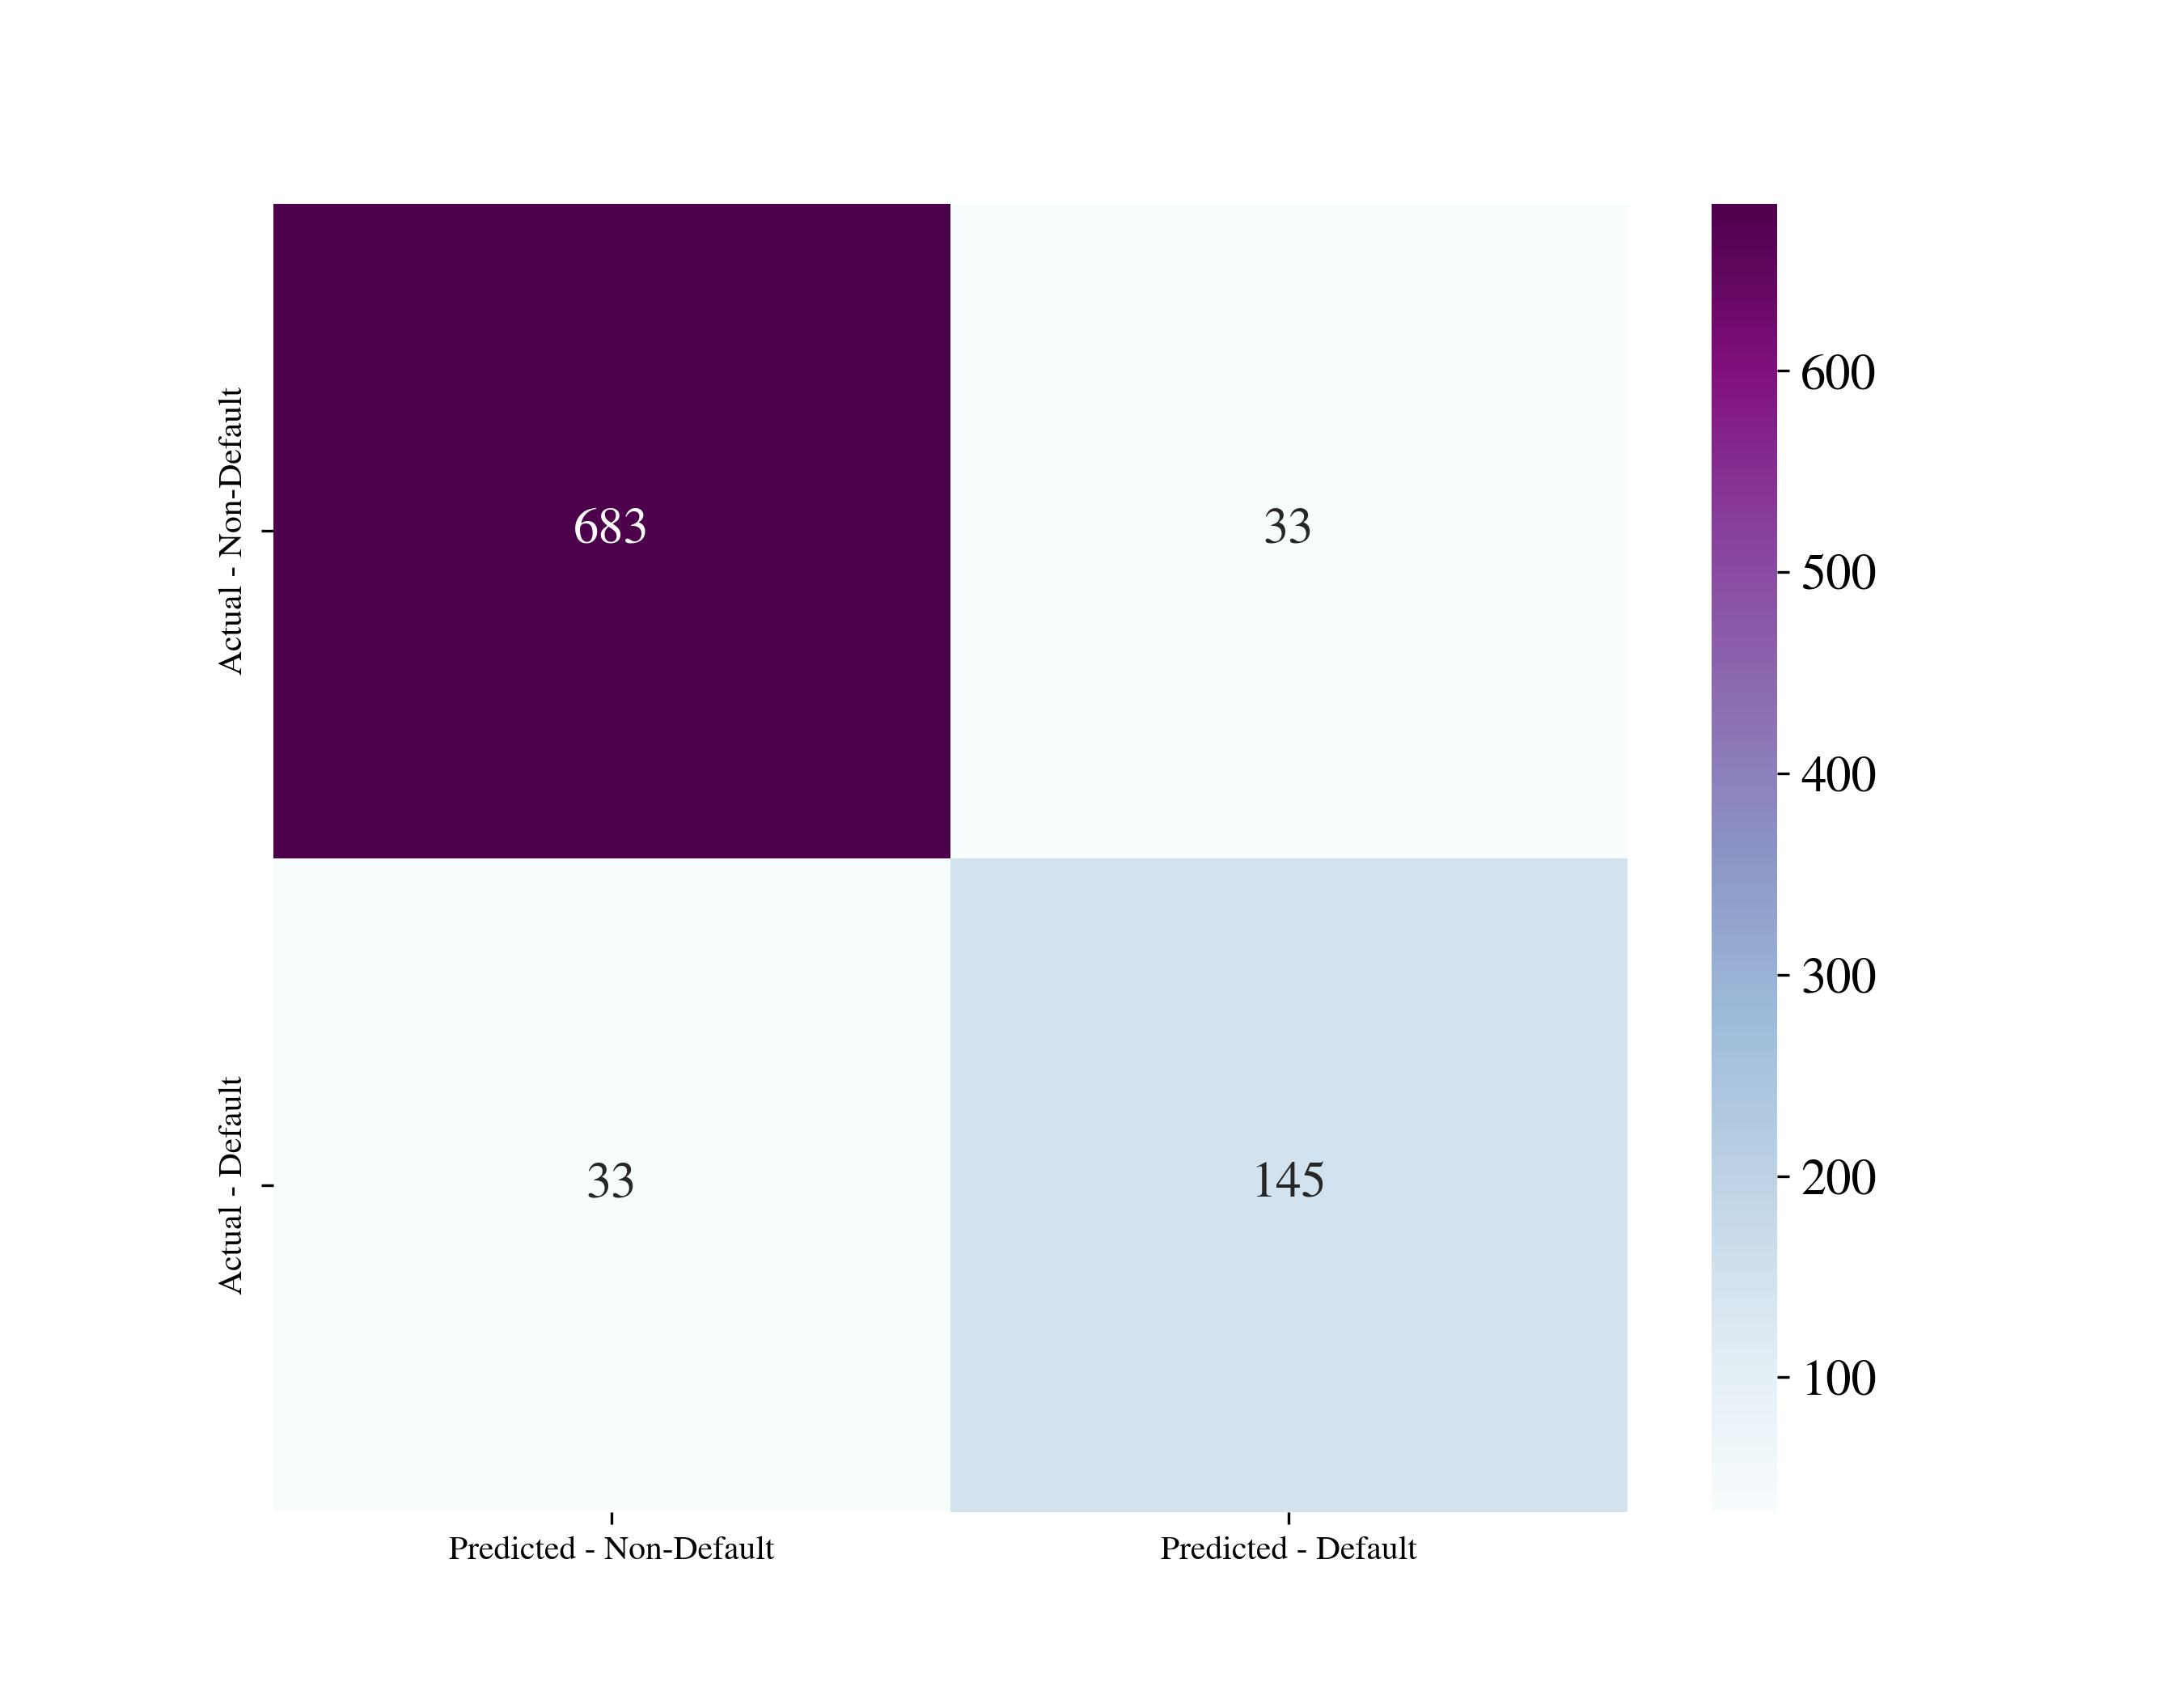
\includegraphics[width=130mm]{Figures/Confusion_Matrix.jpg}
\centering{\begin{source}Author's results in Python\end{source}}\vspace{-1em}
\end{figure}

In order to obtain a better understanding of the model's performance on previously unseen data, we computed several metrics that were used during the model selection process.
These metrics are presented in \autoref{tab:metrics eval}. The results indicate that the model performs well on the unseen data, with most of the scores metrics around 80 \% to 90 \%.
Furthermore, the loss metrics are relatively low, indicating that the model can effectively distinguish between defaults and non-defaults.
Overall, these results suggest that the model is performing well and is suitable for predicting defaults.
The results suggest that the model has a good balance between correctly identifying defaults and non-defaults, as well as minimizing false positives and false negatives. This further confirms the model's ability to accurately predict defaults.
\begin{table}[H]
    \small
    \setlength{\tabcolsep}{8pt}
    \renewcommand{\arraystretch}{1.3}
    \centering
        \caption[Metrics Evaluation]{Metrics Evaluation}\label{tab:metrics eval}
        \begin{tabular}{@{} r r @{\hspace{1cm}} l @{}}
    \toprule
    \textbf{Metric} & \textbf{Value}\\
    \midrule
    \hline
    F1 & 0.8146 \\ 
    Precision & 0.8146 \\ 
    Recall & 0.8146 \\ 
    Accuracy & 0.9262 \\ 
    AUC & 0.9564 \\ 
    Somers D & 0.9128 \\ 
    KS & 0.7915 \\ 
    MCC & 0.7685 \\ 
    Jaccard Score & 0.6872 \\
    Brier Score Loss & 0.0594 \\
    Log Loss & 0.2163 \\
    \hline
    \bottomrule
    \end{tabular}
    \vspace{0.35em}

        \centering{\begin{source}Author's results in Python\end{source}}\vspace{-1em}
\end{table}

To further evaluate the performance of the model, we can visualize the Receiver Operating Characteristic (ROC) curve, as presented in \autoref{fig:roc}. The curve illustrates the trade-off between the true positive rate and the false positive rate at various classification thresholds. An ideal ROC curve should have an area under the curve (AUC) value of 100 \%, indicating a perfect classifier, while a random classifier would have an AUC of 50 \%.

From the curve, we observe that the AUC value of the model is 95.55 \%, indicating a high degree of accuracy in distinguishing between defaults and non-defaults. The curve covers most of the area under the diagonal line, indicating that the model is performing well in differentiating the two classes. Therefore, the results suggest that the model is performing well and is capable of accurately identifying potential defaulters.

\begin{figure}[H]
\centering
\caption{ROC Curve}\vspace{0.5em}
\label{fig:roc}\
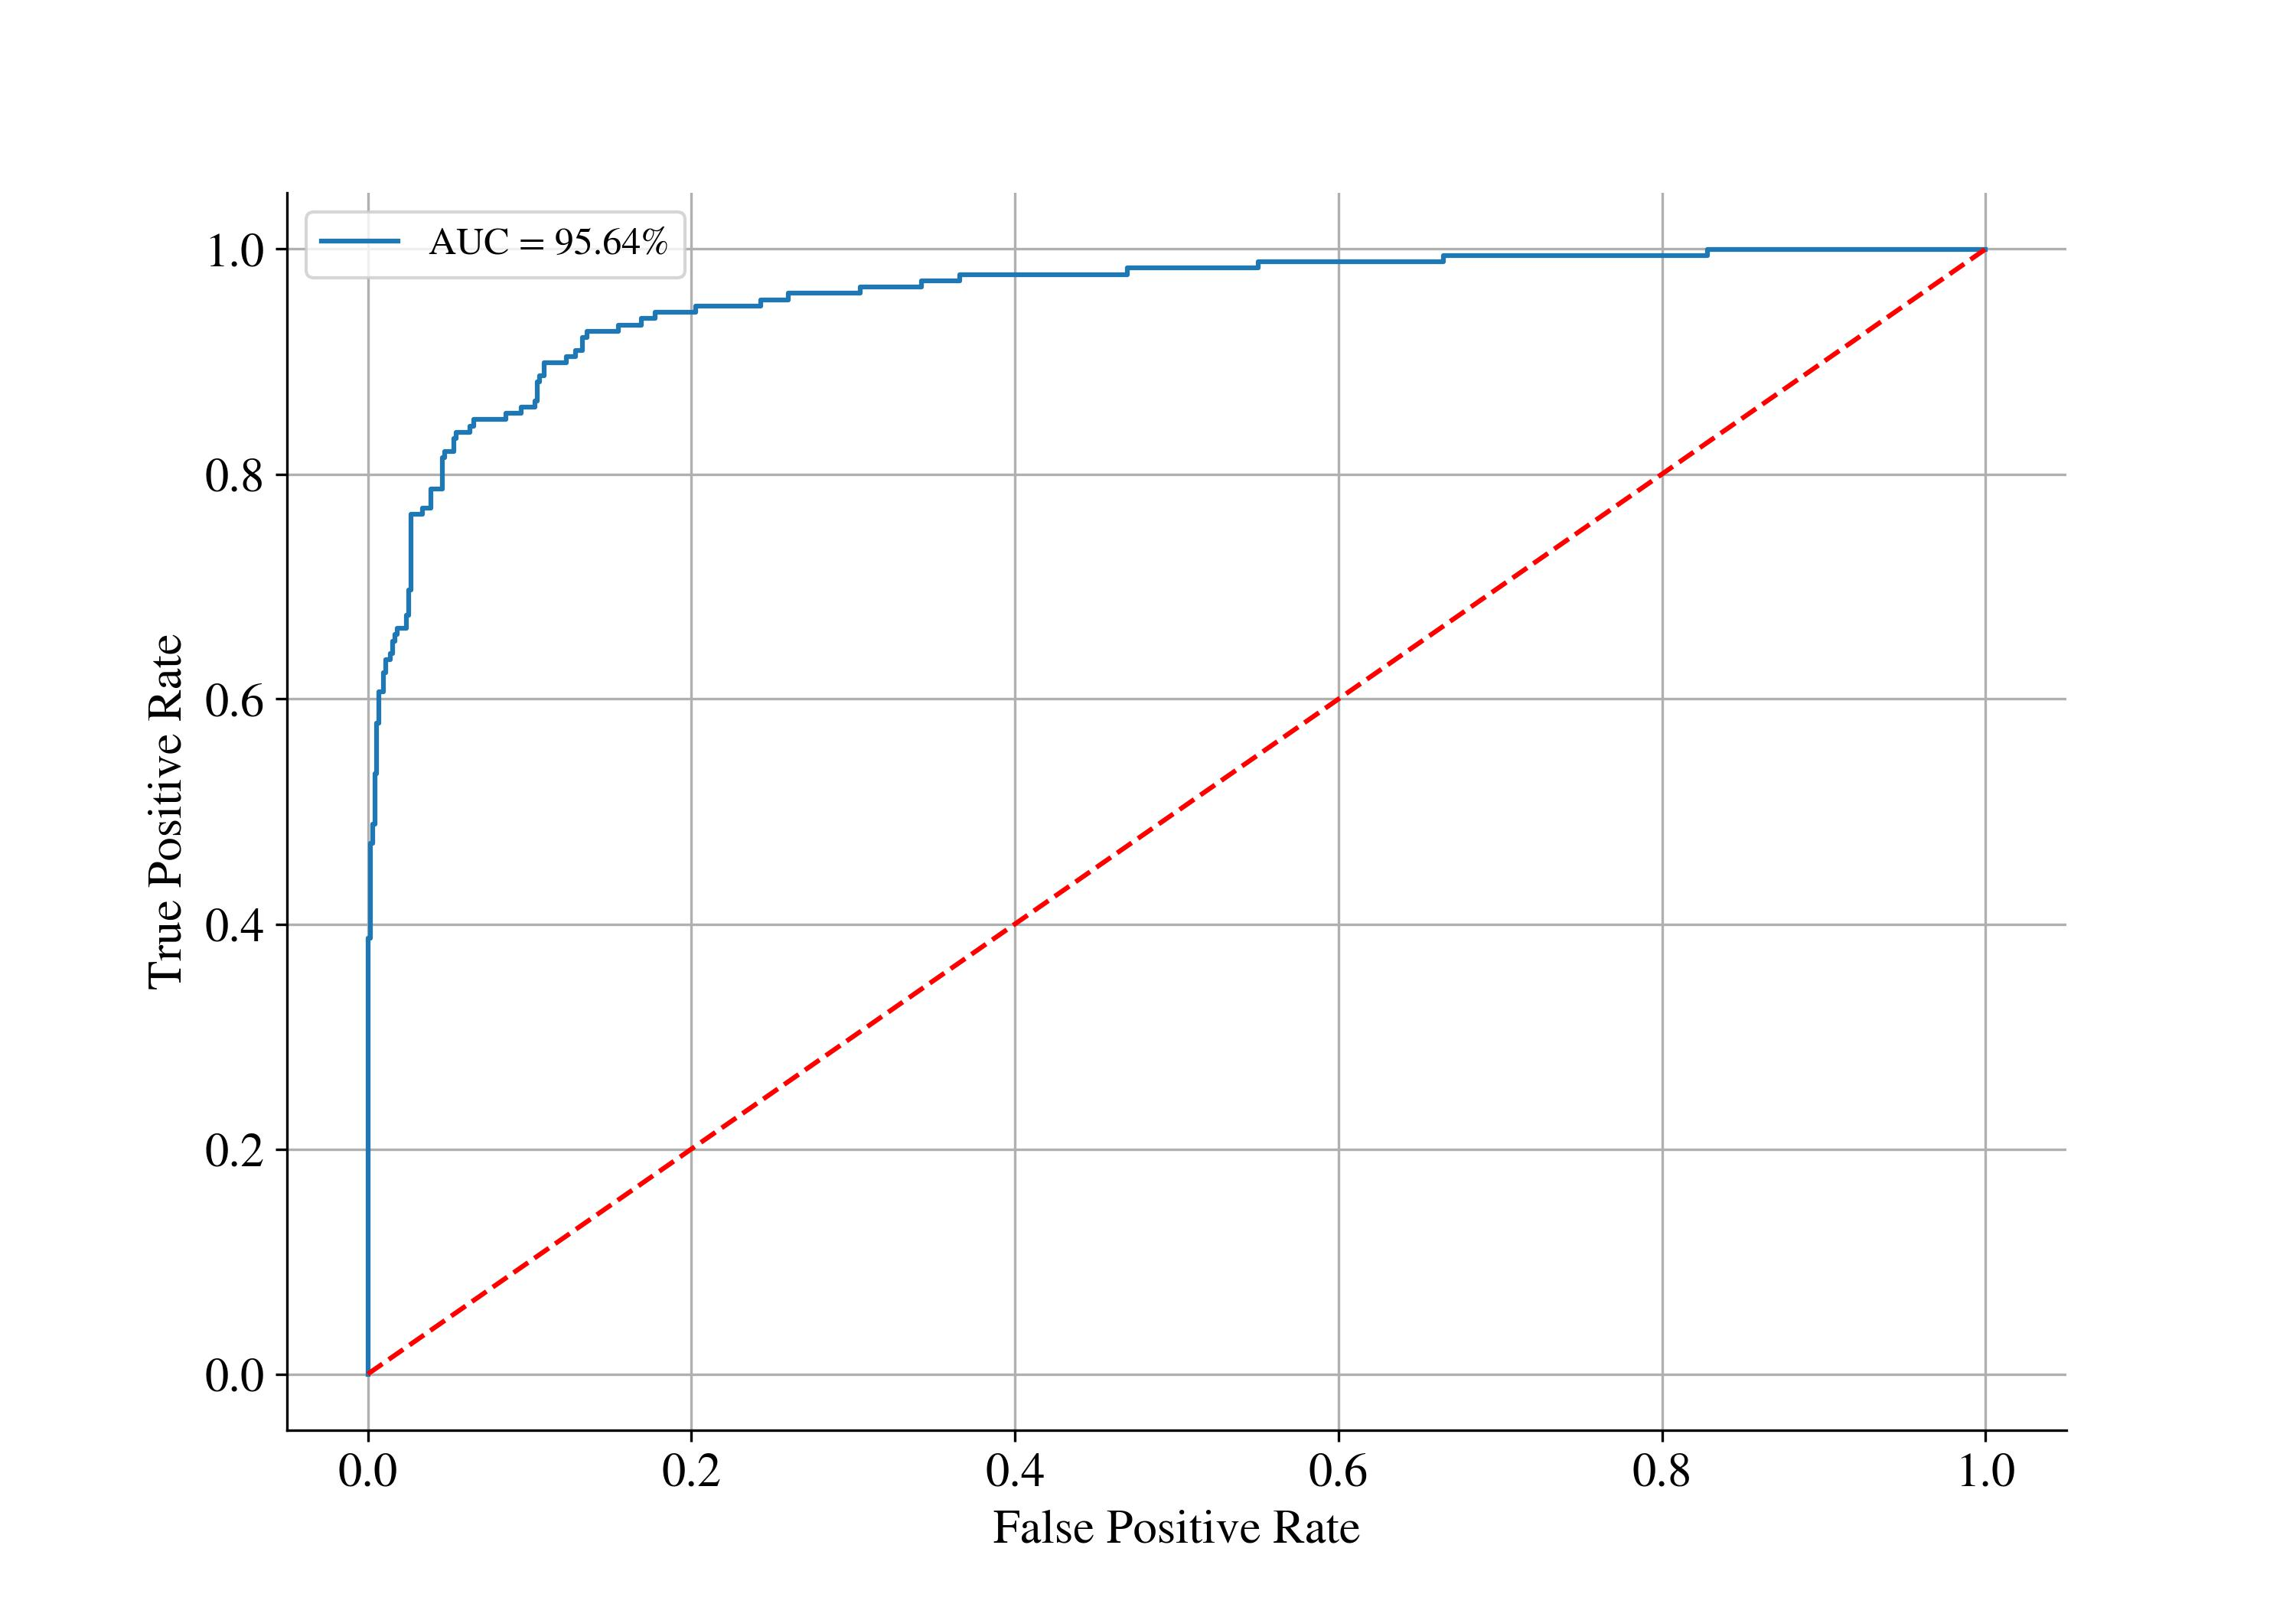
\includegraphics[width=140mm]{Figures/ROC_curve_FINAL.jpg}

\centering{\begin{source}Author's results in Python\end{source}}\vspace{-1em}
\end{figure}
To gain insights into the impact of the features used in the final model, a feature importance graph was visualized and is presented in \autoref{fig:fi}.
Feature importance is a measure of how much a feature contributes to the overall performance of the model, and it is based on the reduction in impurity achieved by splitting the data on that feature.
The higher the reduction in impurity, the more important the feature is considered to be.
Overall, the feature importance plot provides valuable insights into the factors that are most important in predicting loan defaults. It can be used to identify which features are contributing the most to the model's accuracy and to guide future feature selection efforts.
The two most important features used in the final model are \texttt{DEBTINC} and \texttt{DEROG}, which are crucial delinquency indicators in determining whether a borrower would be able to repay their loan. These two features have a significant impact on the model's ability to accurately predict loan defaults, with high feature importance scores.

Understanding the impact of individual features on model performance can be useful in identifying areas for improvement, as well as in identifying the most significant factors that drive loan defaults.
By focusing on these important features, lenders and policymakers can better understand and address the underlying factors that contribute to default risk, ultimately leading to better lending decisions and improved outcomes for borrowers and lenders alike.

\subsection{Model Explainability}

\begin{figure}[H]
\centering
\caption{Feature Importance}\vspace{0.5em}
\label{fig:fi}\
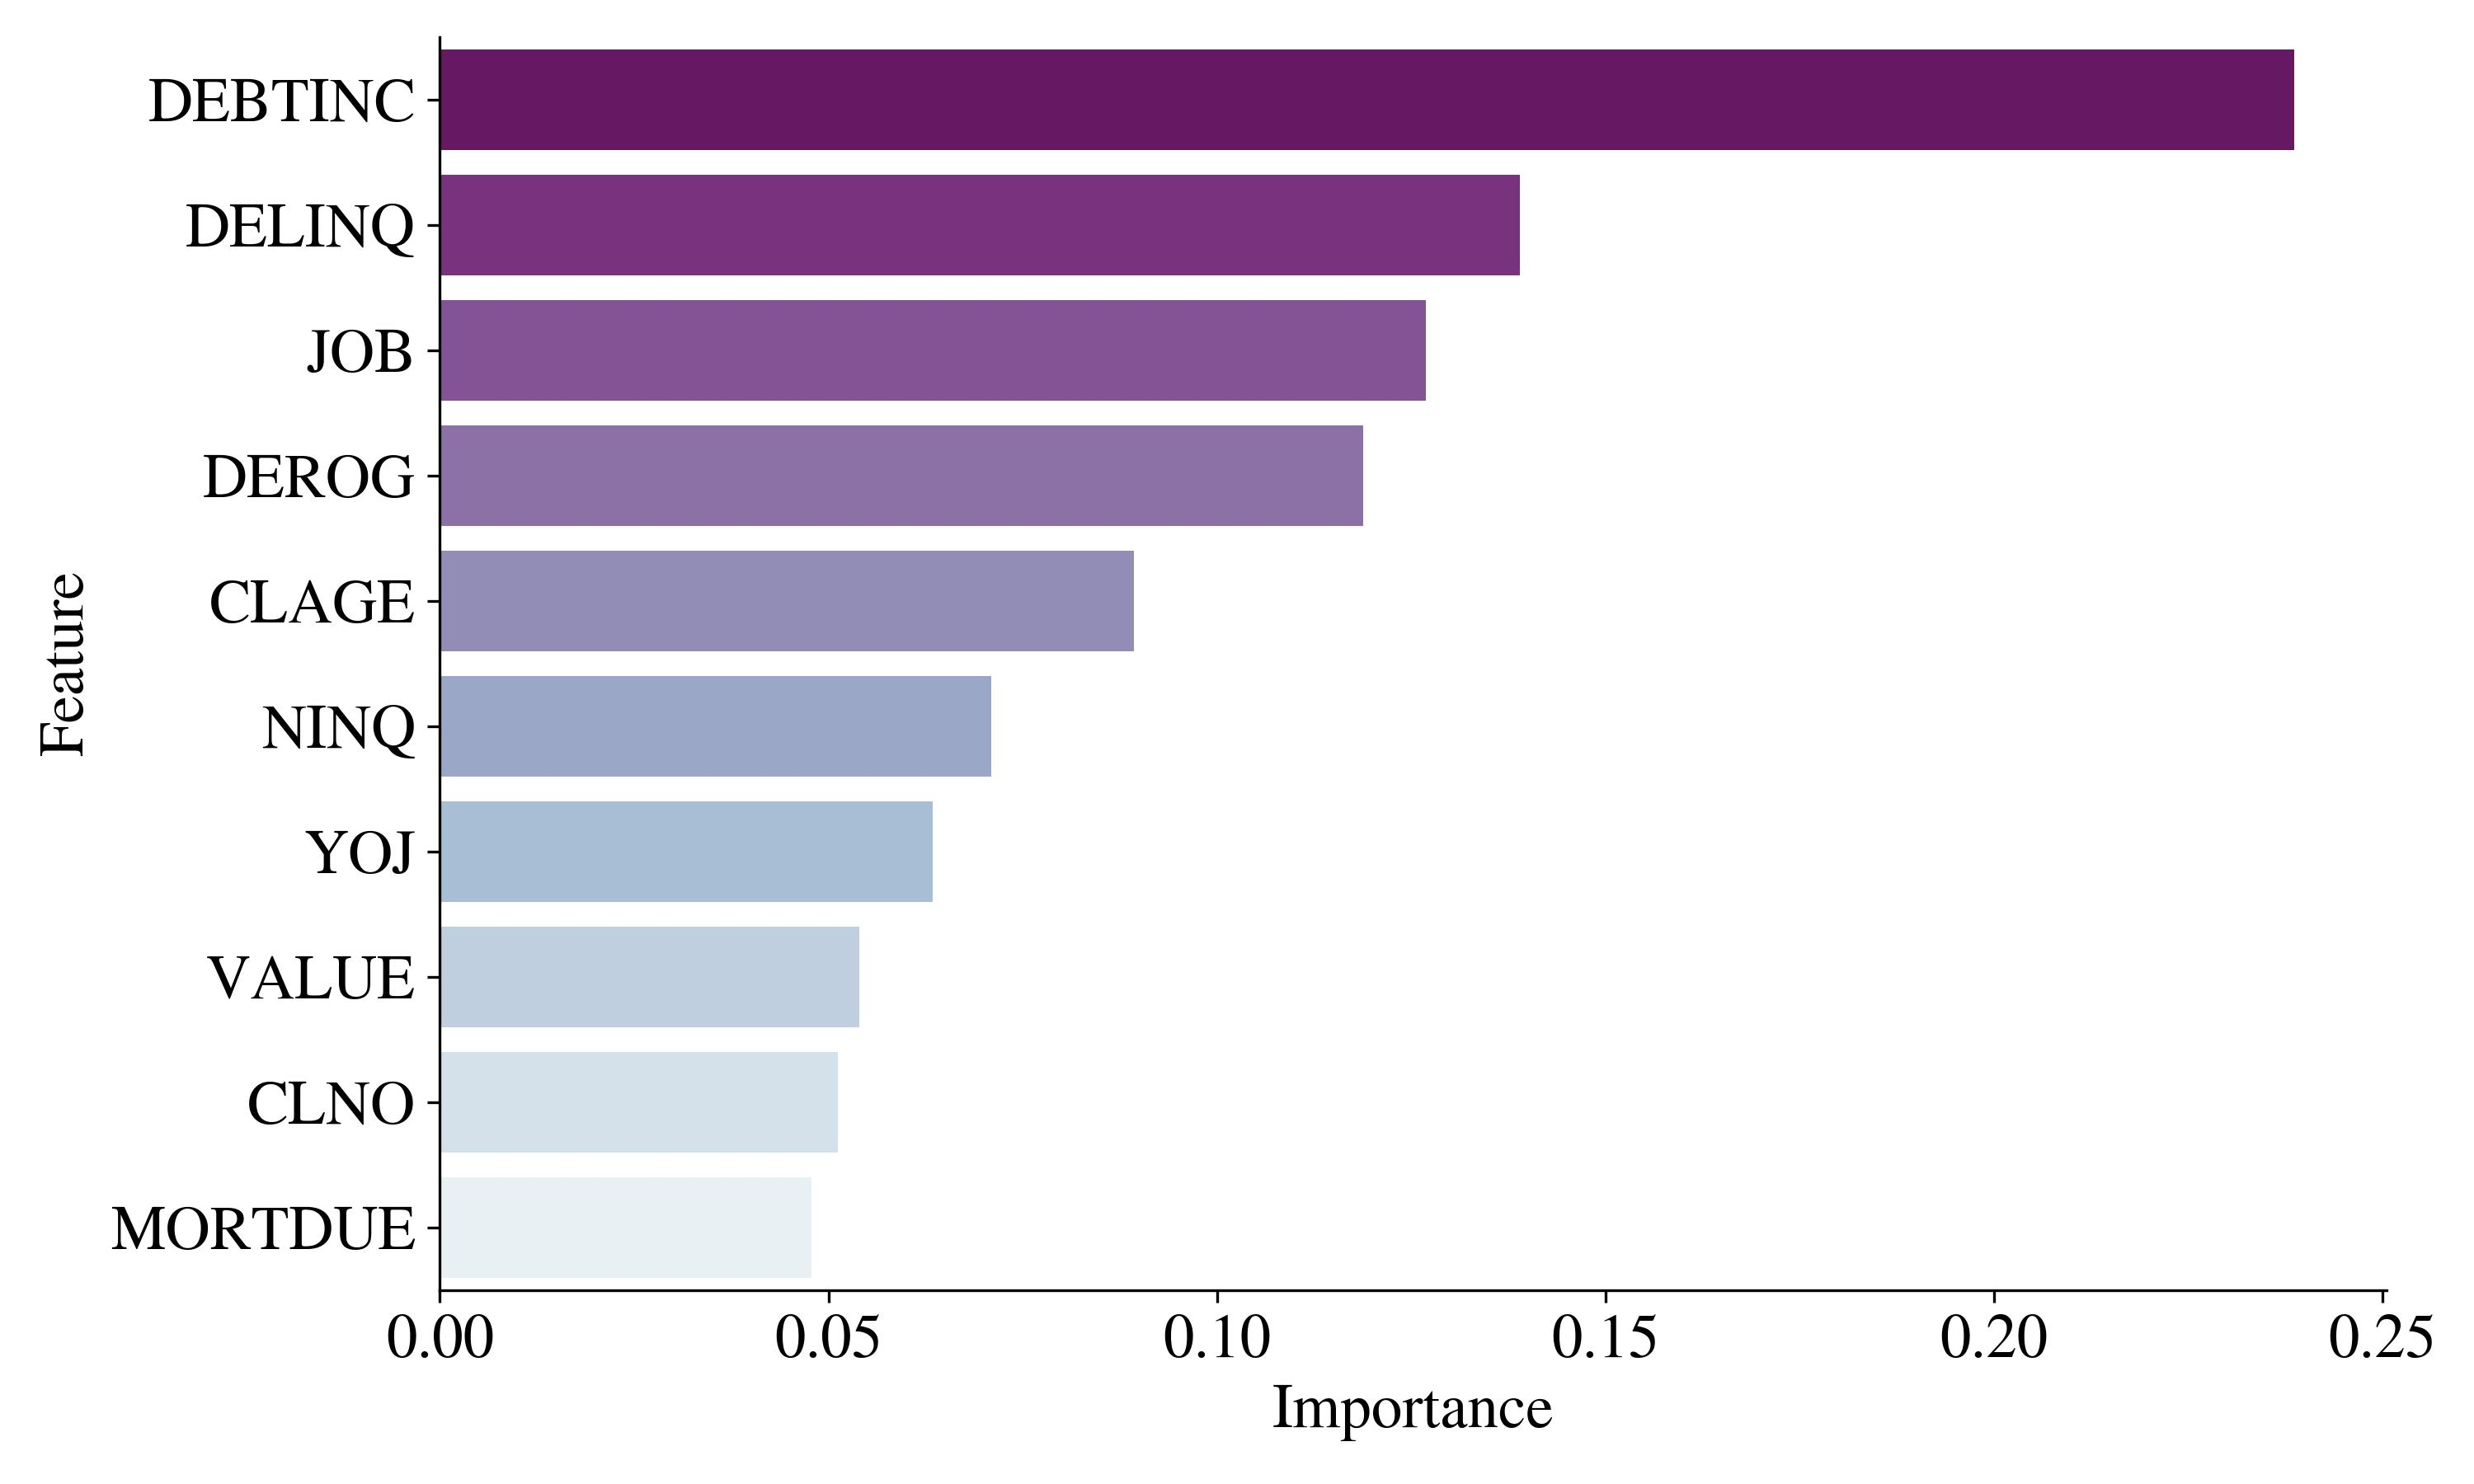
\includegraphics[width=140mm]{Figures/Feature_Importances.jpg}
\centering{\begin{source}Author's results in Python\end{source}}\vspace{-1em}
\end{figure}

To gain further insights into the impact of the features on the final model's predictions, the SHAP (SHapley Additive exPlanations) summary plot is displayed in \autoref{fig:shap}.
The SHAP summary plot provides a clear visualization of the contribution each feature makes to a prediction and is used for a black box model explainability.
Each dot in the plot represents a feature and its corresponding SHAP value.
The color of the dot represents the feature's value, with red indicating high values and blue indicating low values.
The position of the dot on the x-axis represents the impact of the feature on the prediction, with features on the right-hand side contributing more positively to the prediction, and features on the left-hand side contributing more negatively.

Since our data points are encoded in WoE values, the higher (the more positive) value, the larger distribution of non-defaulters compared to defaulters, and vice versa, the lower (the more negative) value, the larger distribution of defaulters compared to non-defaulters.
For the most important features, we can observe that the blue values (negative WoE values) and red values (positive WoE values) are quite separable.
Negative WoE values are positively contributing to the predictions, and the positive WoE values are negatively contributing to the predictions. This means that the more negative the WoE value, the more likely the borrower is to default, and vice versa.

Overall, the SHAP summary plot provides a valuable tool for interpreting and understanding the complex decision-making process of the final model.
The plot enables us to examine the impact of individual features on the model's output and helps us to identify which features are most influential in the model's decision-making process.
By understanding the relative importance of each feature, we can gain deeper insights into the creditworthiness assessment process and make more informed decisions in the lending industry.

\begin{figure}[H]
\centering
\caption{SHAP Summary Plot}\vspace{0.5em}
\label{fig:shap}\
\includegraphics[width=140mm]{Figures/SHAP_summary_plot.jpg}
\centering{\begin{source}Author's results in Python\end{source}}\vspace{-1em}
\end{figure}

\section{Machine Learning Deployment}
This section describes the process of taking a trained machine learning model and making it available for use in the real world. It involves taking the model from a development environment and integrating it into a production environment where it can be used to make predictions or decisions based on new data. In this thesis, the machine learning model is deployed as web application using Flask and HTML.
\subsection{Final Model Recalibration}
Before deploying the model in a production setting, a meticulous process is undertaken to ensure optimal performance.
This involves conducting a final recalibration of the model using the entire dataset, comprising the training, validation, and test sets.
The purpose of this recalibration is to fine-tune the model parameters, thereby maximizing its ability to generalize and yield accurate predictions.

The test set, which has been employed previously during the model evaluation phase, is incorporated into the recalibration process without any risk of data leakage.
By including the test set, the sample size for training is expanded, thereby increasing the model's capacity to generalize effectively.

Upon completion of the recalibration, the final classification threshold for deployment is determined to be \textbf{0.3358}.
This value is derived from a comprehensive analysis of the training, validation, and test sets, which ensures that the model's generalization capabilities are further enhanced for optimal performance in real-world applications.

\subsection{Flask and HTML Web Application}

In this case, the machine learning model was deployed into a web application using Flask and HTML. The application is temporarily deployed on the Cloud server on the \textbf{PythonAnywhere} platform and is accessible here: \url{http://ml-credit-risk-app-petrngn.pythonanywhere.com/}.
However, the application will be shut down after the thesis defense and will not be available online anymore due to the budget reasons.
Nevertheless, the code for the application is available in the GitHub repository, and the application can be run locally using any Python compiler.

Furthermore, prior to deployment, we need to prepare several Python inputs for the web application, including:
\begin{itemize}\setlength\itemsep{0em}
\item Model - the final model recalibrated on the training, validation and test set.
\item Threshold - the final classification threshold recalibrated on the training, validation and test set.
\item Features - the final features used in the final model.
\item Data Frame - he input data frame used in the web application to store the loan applicant's inputs.
\item Optimal Binning Transformator - fitted \lstinline{BinningProcess} object for binning and WoE-encoding of the loan applicant's inputs.
\item WoE Bins - a set of bins and WoE values used for mapping the WoE values to missing values.
\end{itemize}

Such inputs required for the machine learning application are exported in the \lstinline{.pkl} format using the \lstinline{pickle} module. This format allows for efficient and easy-to-use serialization and deserialization of the inputs. The pickled file is then loaded directly into the Flask application.

For the back-end of the web application, Flask is used to deploy the machine learning model. The Flask application is coded in the \lstinline{app.py} file, which is stored in the \lstinline{flask_app} repository. The front-end of the web application is coded in HTML, with CSS and JavaScript elements used to enhance the user interface.

The web application first renders an HTML page, as shown in \autoref{fig:flaskform}.
This page contains a loan application form, in which the user or the loan applicant fills in the respective field values that correspond to the features on which the machine learning model was trained.
The form is designed to capture the necessary information required for the model to make a prediction about the loan applicant's application.
Note that not all fields in the loan application form need to be filled out, except for the requested loan amount. This is because missing values in certain features may indicate a higher risk of defaulting. Conversely, one may choose to impose a restriction on the form, requiring all fields to be filled out. However, this could result in a lower number of received applications from delinquent clients, as they may not have all the necessary information to complete the form.

\begin{figure}[H]
\centering
\caption{Flask Web Application Form}\vspace{0.5em}
\label{fig:flaskform}\
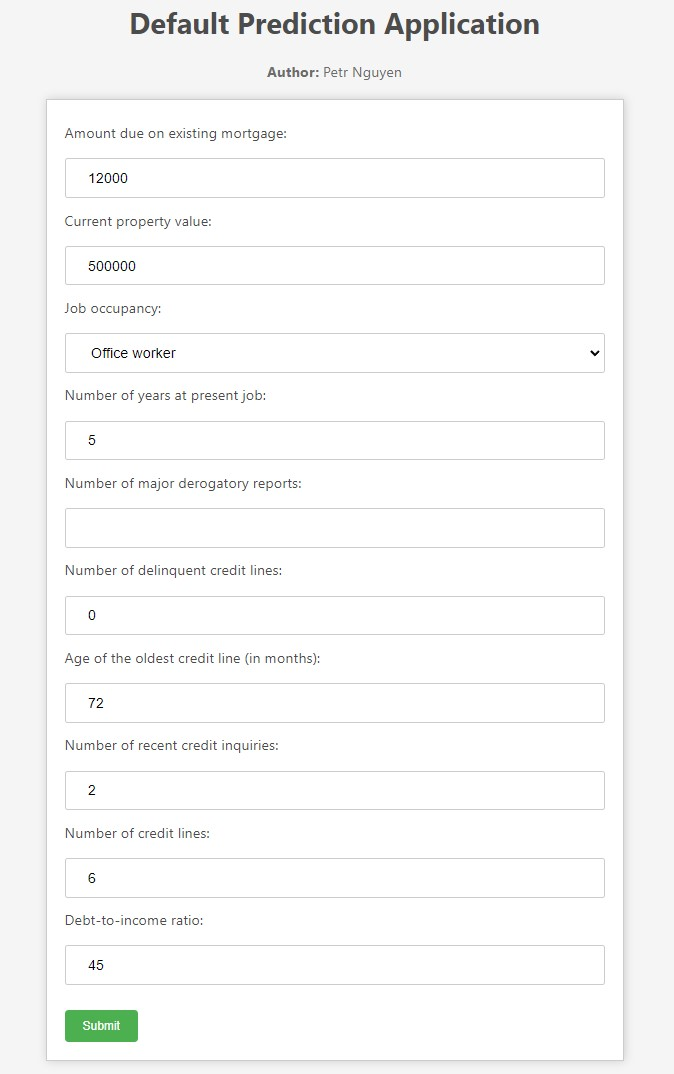
\includegraphics[width=140mm]{Figures/flask_app_form.jpg}

\centering{\begin{source}Author's results in Python\end{source}}\vspace{-1em}
\end{figure}
\clearpage

Once, the loan application form is submitted, the web application uses the pickled input to transform the data from the loan application form and use it in the recalibrated model in order to get the result, whether the given loan applicant would repay his loan based on predetermined threshold. The result is then displayed in the web application, as shown in \autoref{fig:flaskres}.
Particularly, the web application returns whether the loan application would be denied or approved and also the probability score of default.

\begin{figure}[H]
\centering
\caption{Flask Web Application - Prediction Result}\vspace{0.5em}
\label{fig:flaskres}\
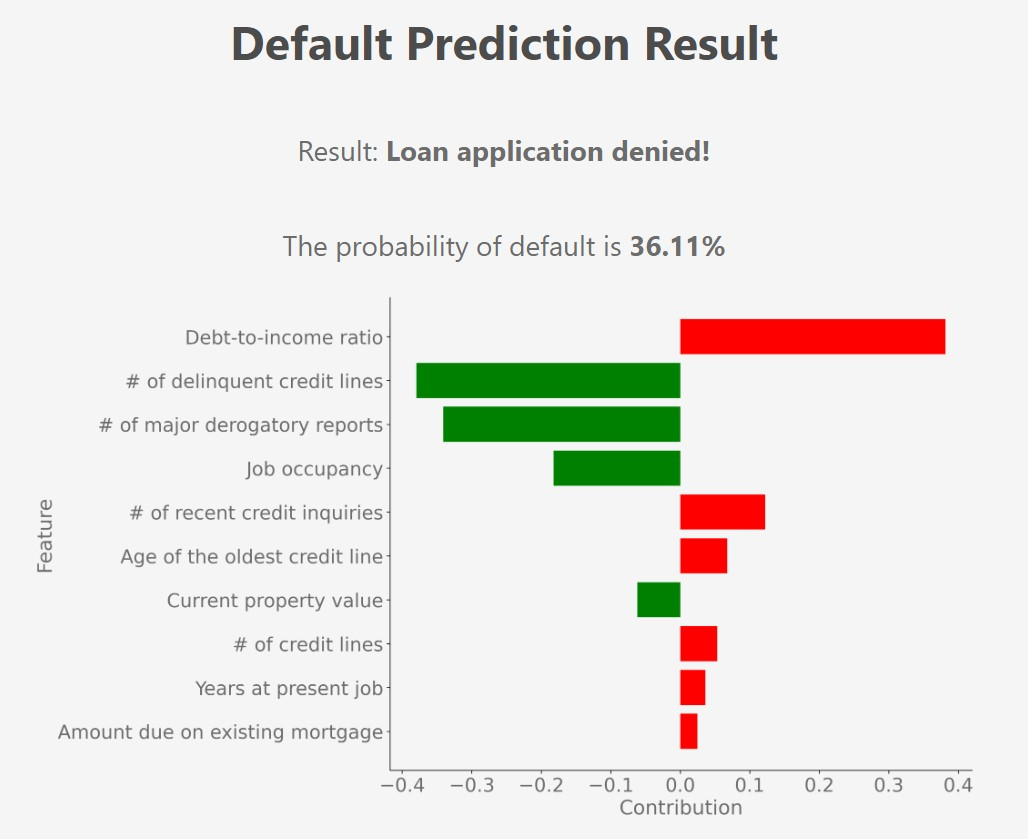
\includegraphics[width=130mm]{Figures/flask_app_result.jpg}

\centering{\begin{source}Author's results in Python\end{source}}\vspace{-1em}
\end{figure}

Besides the prediction results, it also displays the Local Interpretable Model-Agnostic Explanations (LIME) of the black--box model (Gradient Boosting) with respect to the inputs submitted within the form.
LIME focuses on the local explainability of the black box model around the black--box prediction as it generates a new dataset consisting of perturbed samples around the given prediction and then trains a surrogate linear model on the new dataset.
Such local interpretable, surrogate model should be a good approximation of the black box model in the vicinity of the given prediction, i.e., the local interpretable model is then used to explain the prediction of the black box model \citep{ribeiro2016should}.

The LIME explanation of input instances $x$ is given as follows:
\begin{equation}\label{eq}
\xi(x) = \arg\min_{g \in G} L(f, g, \pi_x) + \Omega(g)
\end{equation}

where $f$ is the original black--box model, $g$ is the surrogate model, $L$ is the loss functions measuring how far is the explanation $\xi(x)$ far from the prediction produced by black--box model $f$, and $\Omega(g)$ is the complexity of the surrogate model $g$.


The explanation is given in terms of the feature importance, which is represented by the magnitude of the feature's coefficient in the local interpretable model. The higher the magnitude of the coefficient, the more important the feature is in the prediction of the black box model.
Therefore, as it is shown in \autoref{fig:flaskres}, the red bars indicate positive contribution to the probability of default whereas green bars indicate negative contribution to the probability of default. In other words, The features with red bars indicates that the client would not probably repay his loan and vice versa.
The contributions' magnitudes are in line with the findings from feature imporance or SHAP values which is focused on the global explainability of the black--box model (not local explainability), that features such as debt--to--income ratio (\texttt{DEBTINC}) or number of deliquent credit lines (\texttt{DELINQ}) have the largest impact of the probability default.
Particularly, a high value of debt--to--income ratio causes higher probability default, whereas no delinquent credit lines leads to the lower probability default.

\chapter{Empirical Analysis - Machine Learning Implementation}
\label{chap:four}
This chapter focuses on the main part of this thesis, particularly on the practical example of machine learning implementation. The machine learning framework deployed in this thesis is shown in \autoref{fig:mlframe}.
\begin{itemize}\setlength\itemsep{0em}
\item \textbf{Data Exploration} - Focus on the exploration of the data in order to infer some insights about the data quality, distribution of the variables, statistical testing or association analysis.
\item \textbf{Data Split} - Focus on the splitting of the data which are used separaterly in diferrent tasks such as model training, hyperparameter tuning, feature selection, model selection and model evaluation.
\item \textbf{Optimal Binning and WoE Encoding} - Focus on the optimal binning and the WoE encoding of the features as the main part of the feature preprocessing.
\item \textbf{Feature Selection} Focus on the feature selection in order to reduce the dimensionality of the data and to improve the performance of the machine learning models - each input model is tuned with Bayesian Optimization.
\item \textbf{Model Selection} -Focusd on the model selection in order to find the best model based on the ranking - each input model is tuned with Bayesian Optimization on the subsets of selected features.
\item \textbf{Model Recalibration (Evaluation)} - Focus on the recalibration of the final model by re-training it on the joined training and validation sets, which will be further evaluated.
\item \textbf{Model Evaluation} - Focus on the evaluation of the final model on the unseen data from test set in order to assess model's predictive power.
\item \textbf{Model Recalibration (Deployment)} - Focus on the final recalibration of the final model by re-training it on the joined training, validation and test sets, which will be further deployed into a production.
\item \textbf{Model Deployment} - Focus on the deployment of the final model into a production as a web application.
\end{itemize}

\begin{figure}[H]
\centering
\caption{Machine Learning Framework}\vspace{0.5em}
\label{fig:mlframe}
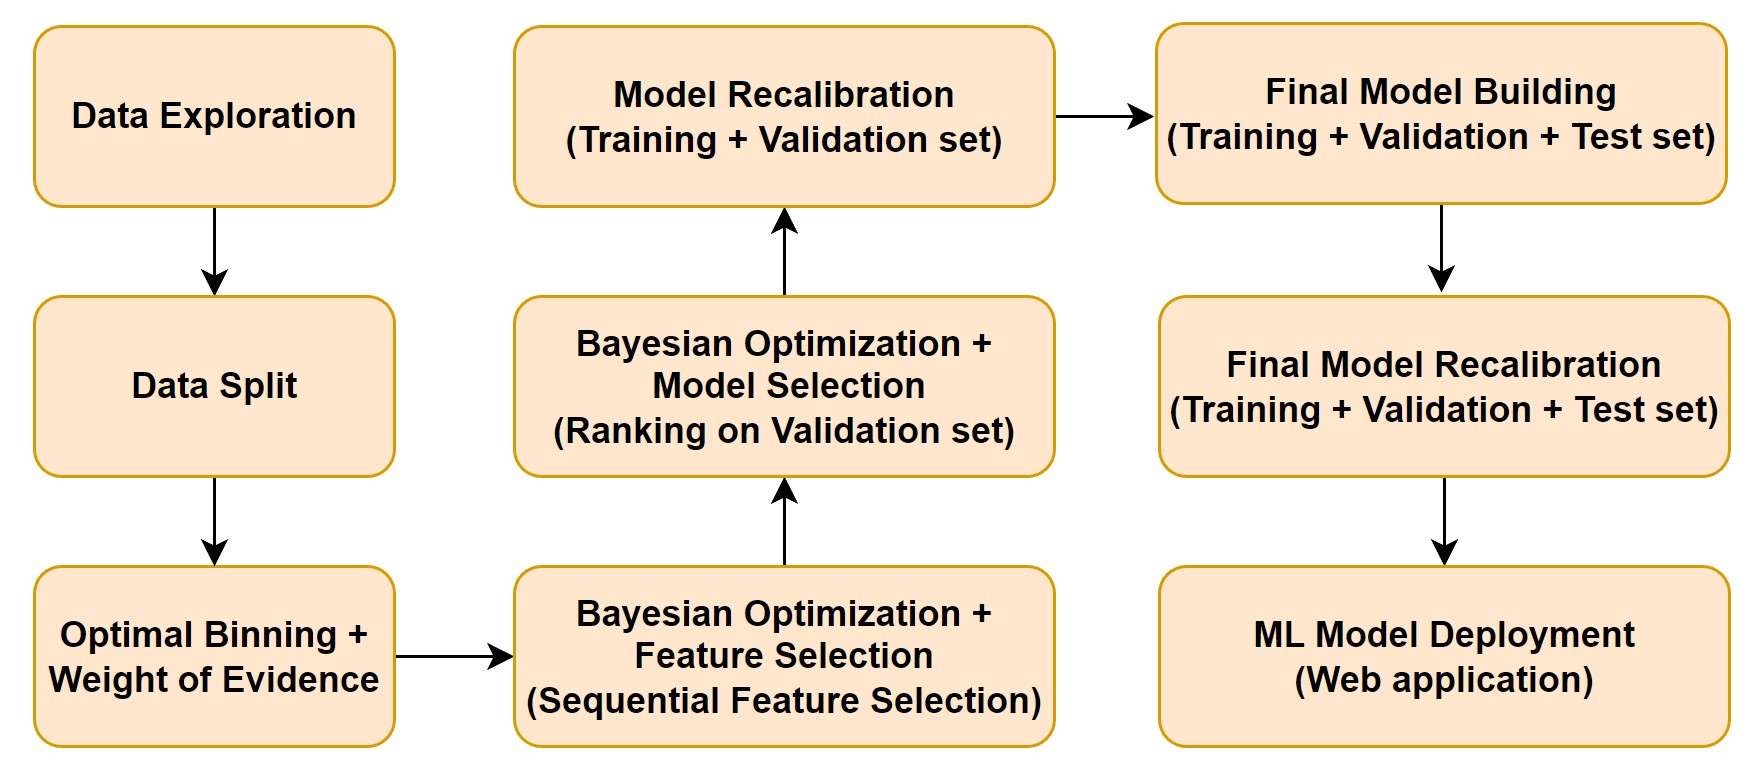
\includegraphics[width=120mm]{Figures/ml_framework.jpg}

\centering{\begin{source}Author's Framework\end{source}}\vspace{-1em}
\end{figure}

\newpage
\section{Repository and Environment Structure}

The whole machine learning implmenetation as the scope of this thesis is done mainly using Python Programming Language and further with collaboration of Git and HTML.
The whole repository can be found in the separate appendix or is available on the GitHub repository \url{https://github.com/petr-ngn/FFU_VSE_Masters_Thesis_ML_Credit_Risk_Modelling}.
The repository structure is shown in \autoref{fig:repostructure}.
\begin{figure}[H]
\centering\caption{Repository Structure}
\label{fig:repostructure}

{\footnotesize
\begin{verbatim}

            |--- data
            |  |--- interim_dat.csv
            |  |--- preprocessed_data.csv
            |  |--- raw_data.csv
            |
            |--- flask_app
            |  |--- inputs
            |  |  |--- inputs_flask_app_dict.pkl
            |  |
            |  |--- templates
            |  |  |--- index.html
            |  |  |--- results.html
            |  |
            |  |--- static
            |  |
            |  |--- app.py
            |
            |--- models
            |  |--- feature_preprocessing
            |  |--- feature_selection
            |  |--- model_selection
            |  |--- objects_FINAL
            |
            |--- plots
            |--- Masters_Thesis.ipynb
            |--- README.md
            |--- requirements.yml
\end{verbatim}
}
\centering{\begin{source}Author's results at GitHub\end{source}}\vspace{0em}
\end{figure}


\begin{itemize}\setlength\itemsep{0em}
\item \texttt{data} - directory containing the raw data, partially preprocessed data (\texttt{interim}) and the final preprocessed data.
\item \texttt{flask\_app} - directory containing the Flask application which is used for the deployment of the model. Particularly, it contains the \texttt{app.py} file which is the main back-end file of the application, the \texttt{templates} and \texttt{static} subdirectories which contain the front-end HTML files for the application, and the \texttt{inputs} subdirectory which contains the input dictionary for the application (such as the trained model, threshold, final features etc.).
\item \texttt{models} - directory containing the the subdirectories of the trained and fitted objects for features preprocessing, feature selection and model selection, including the final objects used in deployment.
\item \texttt{plots} - directory containing the plots generated within the main Python notebook.
\item \texttt{Masters\_Thesis.ipynb} - main Python notebook containing the main part of the machine learning Implementation, such as exploratory analysis, data preprocessing, training and evaluation of the models.
\item \texttt{README.md} - README file containing the description of the repository.
\item \texttt{requirements.yml} - file containing the list of the required packages and their specific versions used in this project.
\end{itemize}

This particular solution is developed in Python version 3.10.9 and these are the main packages and modules used in this project:
\begin{itemize}\setlength\itemsep{0em}
\item \lstinline{NumPy}, \lstinline{Pandas} - for data manipulation and analysis.
\item \lstinline{Matplotlib}, \lstinline{Seaborn} - for data visualization.
\item \lstinline{Scipy} - for statistical analysis.
\item \lstinline{OptBinning} - for optimal binning of features with respect to the target.
\item \lstinline{ImbLearn} - for handling imbalanced data using oversampling.
\item \lstinline{Scikit-learn} - for feature selection, model selection and model evaluation.
\item \lstinline{Scikit-optimize} - for more advanced hyperparameter optimization.
\item \lstinline{Flask} - for deployment of the model as web application.
\end{itemize}

To replicate this solution, one may download this repository as a zip file or either can clone this repository using Git to the local repository. Before running any files or scripts, it is important to set the environment for such project using the file \texttt{requirements.yml}. This can be done by running the following command in the Anaconda terminal which will create the new environment with the name \texttt{FFU\_VSE\_Masters\_Thesis} and install all the required packages:
\begin{figure}[H]
\centering\
{\footnotesize
\begin{verbatim}
>> conda env create -n FFU_VSE_Masters_Thesis -f requirements.yml    
\end{verbatim}
\vspace{-1em}
}
\end{figure}
Be aware of your current path directory in your terminal. In order to install the file \texttt{requirements.yml}, you need to define a path to the directory, where such file is located.
To achieve this, the user has to either change the path in the terminal using \texttt{cd} command, insert the path directory before the \texttt{requirements.yml} in terminal, or to copy the file \texttt{requirements.yml} to the current path directory. The following code shows the former approach:
\begin{figure}[H]
\centering\
{\footnotesize
\begin{verbatim}
>> cd C:\Users\ngnpe\FFU_VSE_Masters_Thesis_ML_Credit_Risk_Modelling
>> conda env create -n FFU_VSE_Masters_Thesis -f requirements.yml   
\end{verbatim}
\vspace{-1em}
}
\end{figure}


To preserve the reproducibility of this solution and conistency of the results, the random seed is instantiated to \texttt{42}, so for instance data split, model optimization or training would be deterministic and not totally random everytime when replicating the solution.

Some \lstinline{Scikit-learn} or \lstinline{Scikit-optimize} objects have optional argument \texttt{n\_jobs} which utilizes the number of CPU cores used during the parallelizing computation. Such argument is set to \texttt{-1}, hence all the processors are used in order to  speed up the training or optimization process.

\newpage
\section{Data Exploration}
This section is focused on exploration of the analyzed loan data set, particularly on data set description, distribution analysis and association analysis, in order to infer potential valuable insights and which can be used in the preprocessing or modelling part.

\subsection{Data Set Description}
\label{subsec:datadescript}
The analyzed data set pertains to the HMEQ data set which contains loan application information and default status of 5,960 US home equity loans. Such data set was acquired from Credit Risk Analytics website \citep{baesens2016credit}. Since this data set regards the loan application scoring data, using macroeconomic or other external data is omitted due to the data set characteristics as well as modelling with behavioral scoring.
Thus our goal is to predict whether the loan applicant will or would default based on provided information from the loan application.

As can be seen in \autoref{tab:dataset}, the data set contains 13 columns, 12 features and 1 target variable \texttt{BAD} indicating whether the loan was in default (\texttt{1}) or not (\texttt{0}). 
Amongst the 12 features, there are 10 numeric features and 2 categorical features, namely \texttt{REASON} which contains 2 categories - Debt consolidation (\texttt{DebtCon}) and Home improvement (\texttt{HomeImp}), and \texttt{JOB} which fontains following categories - Administration (\texttt{Office}), Sales, Manager (\texttt{Mgr}), Professional Executive (\texttt{ProfExe}), Self-employed (\texttt{Self}), and Other.


\begin{table}[H]
\small
\setlength{\tabcolsep}{8pt}
\renewcommand{\arraystretch}{1.3}
\centering
\caption[Data Set Columns]{Data Set Columns}\label{tab:dataset}
\begin{tabular}{@{} l p{8cm} l @{}}
\toprule
\textbf{Variable} & \textbf{Description} & \textbf{Data type}\\
\midrule
\hline
BAD & Default status & Boolean \\

LOAN & Requested loan amount & numeric \\

MORTDUE & Loan amount due on existing mortgage & numeric \\

VALUE & Value of current underlying collateral property & numeric \\

REASON & Reason of loan application & categorical \\
JOB & Job occupancy category & categorical \\

YOJ & Years of employment at present job & numeric \\

DEROG & Number of derogatory public reports & numeric \\

DELINQ & Number of delinquent credit lines & numeric \\

CLAGE & Age of the oldest credit line in months & numeric \\

NINQ & Number of recent credit inquiries & numeric \\

CLNO & Number of credit lines & numeric \\

DEBTINC & Debt-to-income ratio & numeric \\
\hline
\bottomrule
\end{tabular}
\vspace{0.35em}

\centering{\begin{source}\citep{baesens2016credit}\end{source}}\vspace{-1em}
\end{table}

After the initial data inspection, data does not contain any duplicates but does contain missing values, which are summarized in \autoref{tab:natable}.
Most of the missing values are observed within the feature \texttt{DEBTINC} with 1,267 missing observations,
whereas columns indicating default status (\texttt{BAD}) or requested loan amount (\texttt{LOAN}) do not contain any missing values, which is expected as the bank should have the available information about their loans whether they have defaulted or not, and since this data set pertains to the application scoring, when applying for a loan, an applicant should always fill out the requested loan amount.

\begin{table}[H]
\small
\setlength{\tabcolsep}{8pt}
\renewcommand{\arraystretch}{1.3}
\centering
\caption[Missing Values Summary]{Missing Values Summary}\label{tab:natable}
\begin{tabular}{l r r}
\toprule
\textbf{Variable} & \textbf{\# NA's} & \textbf{\% NA's}\\
\midrule
\hline
BAD & 0 & 0.00 \% \\
LOAN & 0 & 0.00 \% \\
MORTDUE & 518 & 8.69 \% \\
VALUE & 112 & 1.88 \% \\
REASON & 252 & 4.23 \% \\
JOB & 279 & 4.68 \% \\
YOJ & 515 & 8.64 \% \\
DEROG & 708 & 11.88 \% \\
DELINQ & 580 & 9.73 \% \\
CLAGE & 308 & 5.17 \% \\
NINQ & 510 & 8.56 \% \\
CLNO & 222 & 3.72 \% \\
DEBTINC & 1267 & 21.26 \% \\
\hline
\bottomrule
\end{tabular}
\vspace{0.35em}

\centering{\begin{source}Author's results in Python\end{source}}\vspace{-1em}
\end{table}


\subsection{Distribution Analysis}
\label{subsec:distribution}
In this subsection, we inspect the distribution of our variables, including the target variable and the features.
Such distribution inspection may help us to identify outliers, and other potential issues with the data set.

\subsubsection{Default Distribution}

Regarding the the target variable distribution, from the \autoref{fig:defaultdist} we can observe that the default status distribution is heavily imbalanced, as most of the loans have not defaulted yet.
Particularly, 80.05\% of the observations have been labelled as non-default (4,771 observations) and 19.95\% observations labelled as default (1,189 observations).
This may cause problems in the modelling part, as the model may be biased towards the majority class, i.e., the non-default class. Such imbalanced class issue will be further treated in \autoref{subsec:data-split-ADASYN}.

\begin{figure}[H]
\centering
\caption{Default Distribution}
\label{fig:defaultdist}
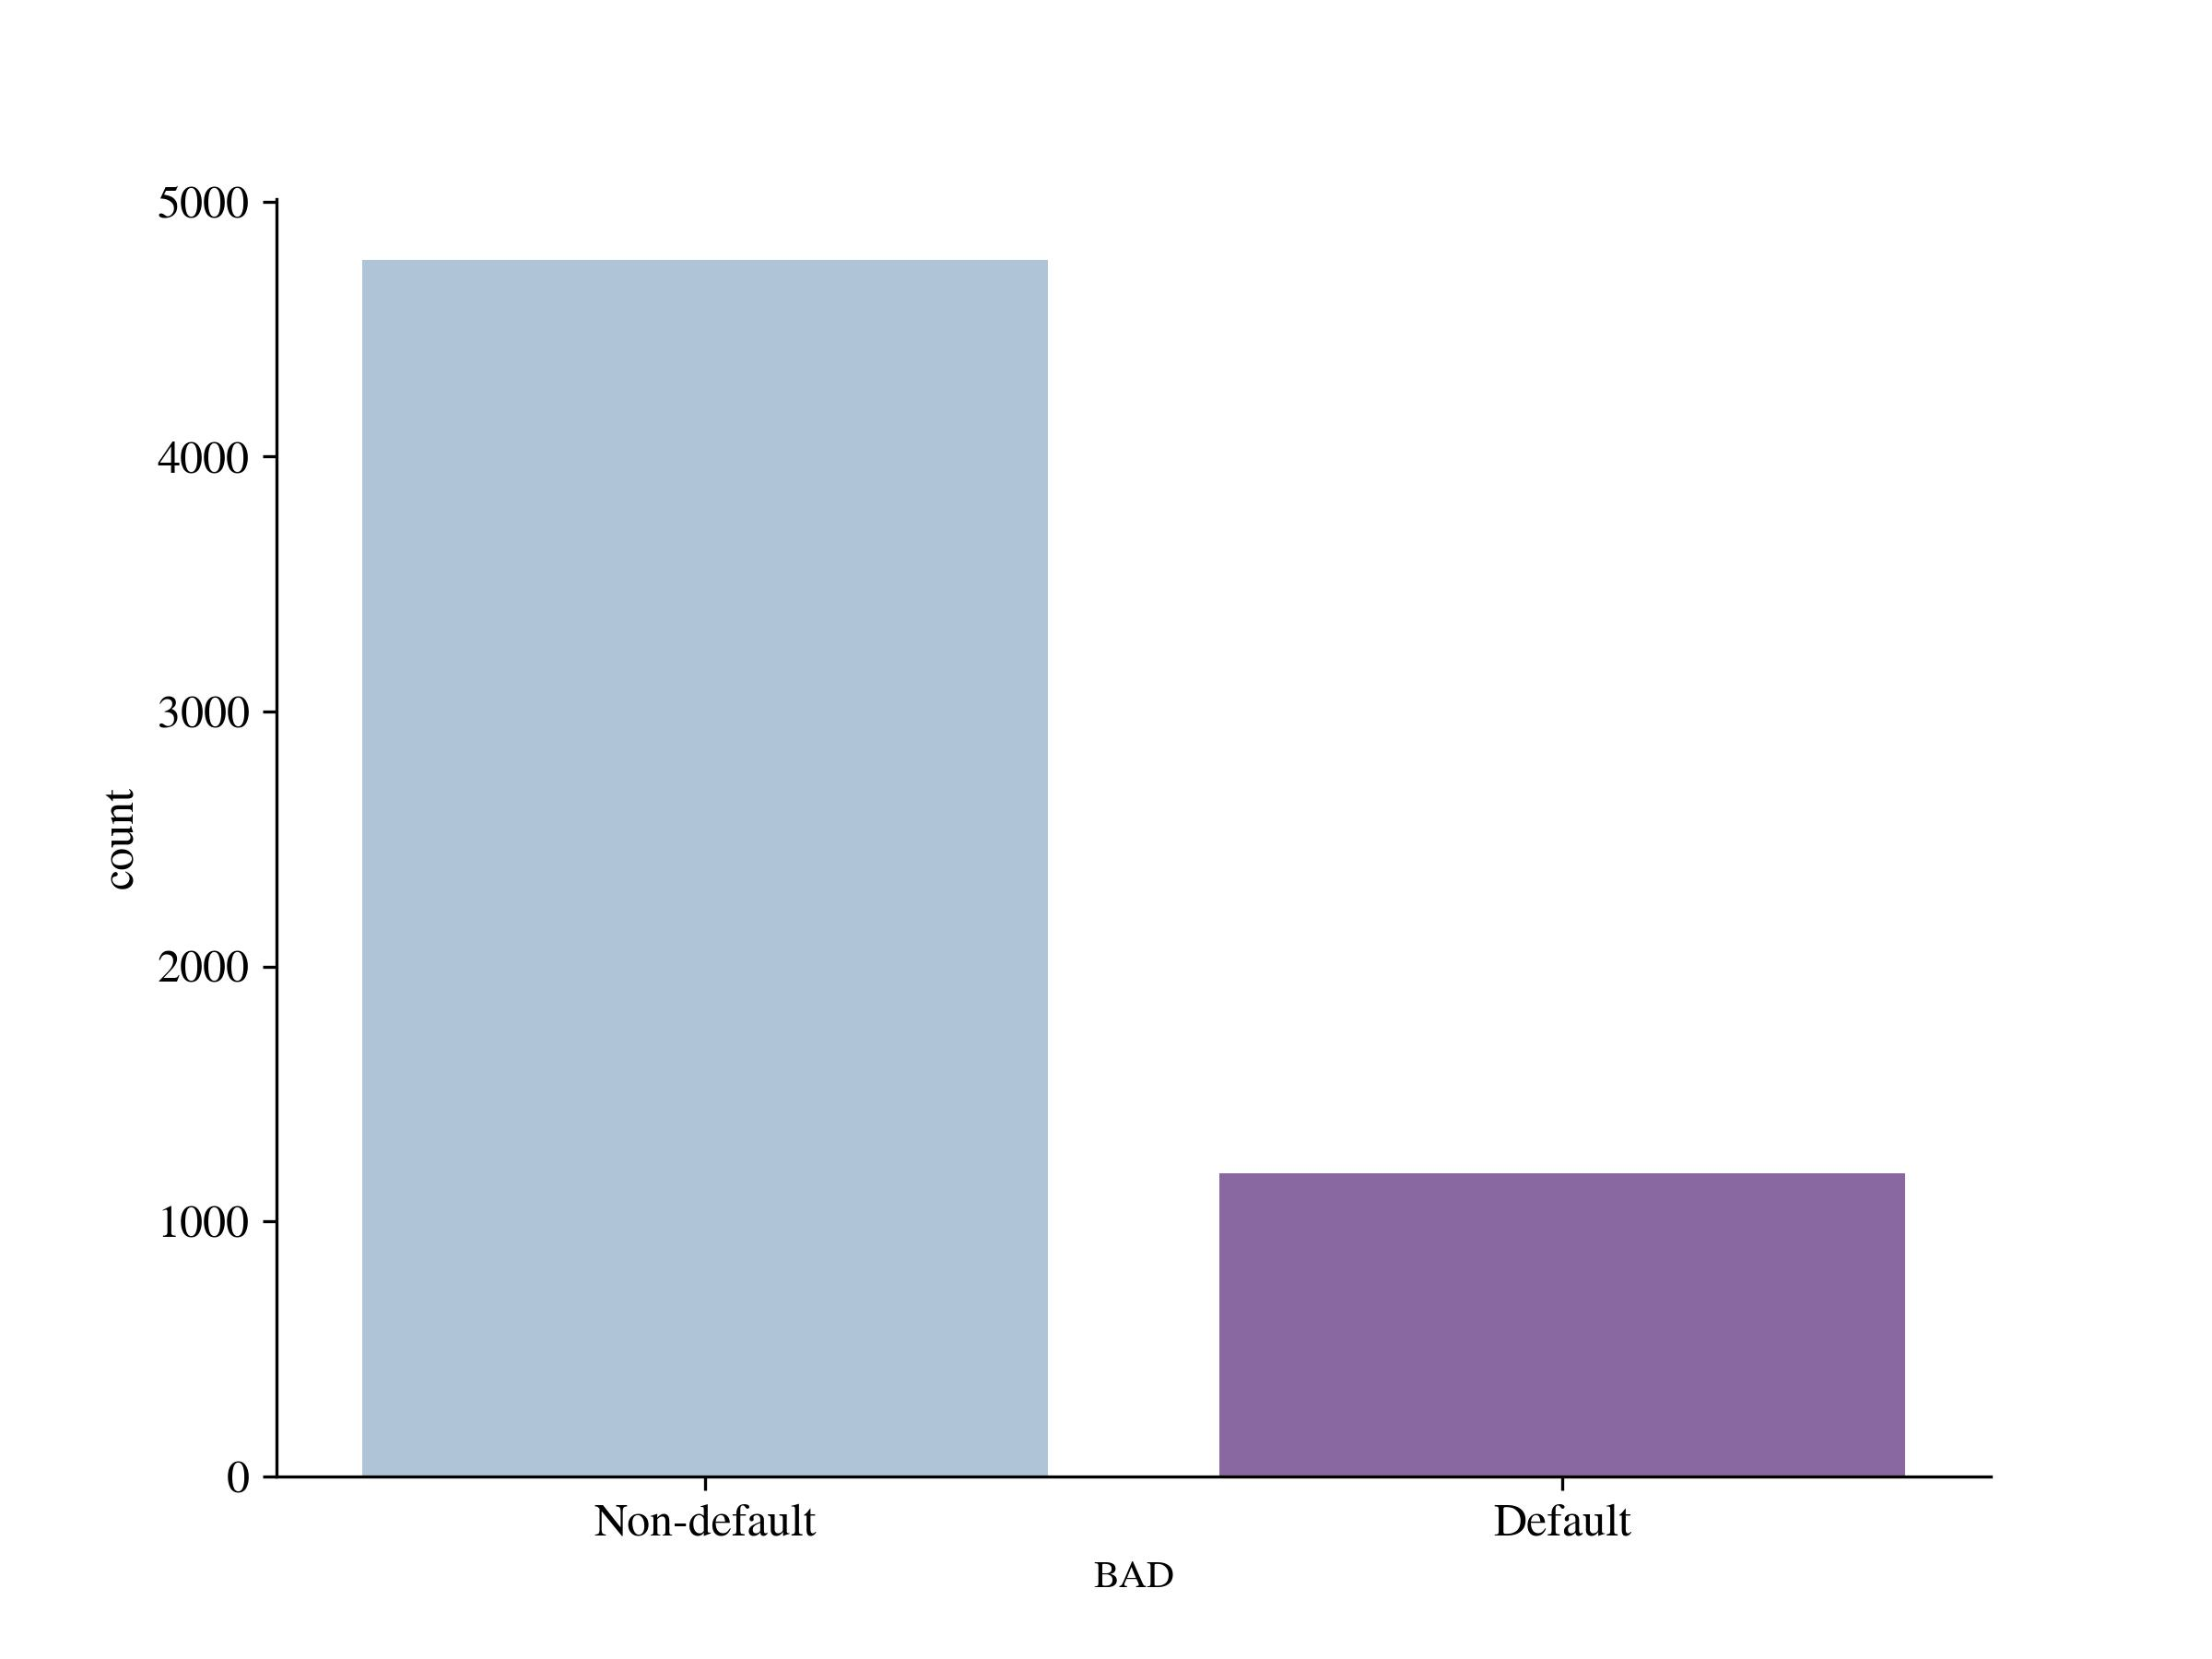
\includegraphics[width=130mm]{Figures/Default_Distribution.jpg}\vspace{-1em}
\centering{\begin{source}Author's results in Python\end{source}}\vspace{-1em}
\end{figure}

\subsubsection{Numeric Features' Distribution}
\label{subsubsec:numdist}

Regarding the numeric features, it can be observed that most of them exhibit a positive skewness and contain outliers, as illustrated in \autoref{fig:boxfeat}, which depicts the conditional distribution of the numeric features with respect to the default status via boxplots.

All the outliers appear to be valid, indicating that they have not arisen due to data entry errors.
This can be attributed to the non-negative nature of all the numeric features, which makes it impossible to have negative values for features such as the number of years at present job or the number of delinquent credit lines, among others.
Additionally, the maximum values of the given features are not unrealistically high, further corroborating the validity of the outliers.
However, it is necessary to treat these outliers as they can bias a model's weights or coefficients, particularly in the case of logistic regression or neural networks.
Outliers can also jeopardize distance calculations in the case of KNN, or in general, affect the position and orientation of the decision boundary.
Such factors can lead to overfitting and inaccurate and biased predictions.
A detailed explanation of the outlier treatment is provided in \autoref{subsec:prep-optbinning}.

Concerning the target variable, it can be observed that there are some differences in the distribution shapes of \texttt{DEROG} and \texttt{DELINQ}, which exhibit less skewness and lower dispersion for non-default cases as compared to default cases.
Since both features indicate negative information about delinquency, it is expected that a higher value for these features would increase the likelihood of loan default.
Referring to the feature \texttt{DEBTINC}, it does not exhibit any extreme values for non-default cases, but some extreme values are present for default cases.
From this, it can be inferred that if the debt-to-income ratio is too high, indicating that the applicant's income is not sufficient to cover their debt, the loan is more likely to end in default.
The association between the default status and the numeric features is further investigated in \autoref{subsubsec:target-num-ass}.

Since the features are positively skewed a lot, they do not follow Guassian (normal) distribution. Additionally, Shapiro--Wilk test is conducted in order to assessed whether the features' distributions are significantly different from a normal distribution.
According to such test, all the numeric features' distributions do not follow normal distribution on 1\% statistical significance level.
For a reference, see \autoref{tab:normalitytest} in \autoref{chap:app1}.

\begin{figure}[H]
\centering
\caption{Conditional Distribution of Numeric Features}\vspace{0.5em}
\label{fig:boxfeat}
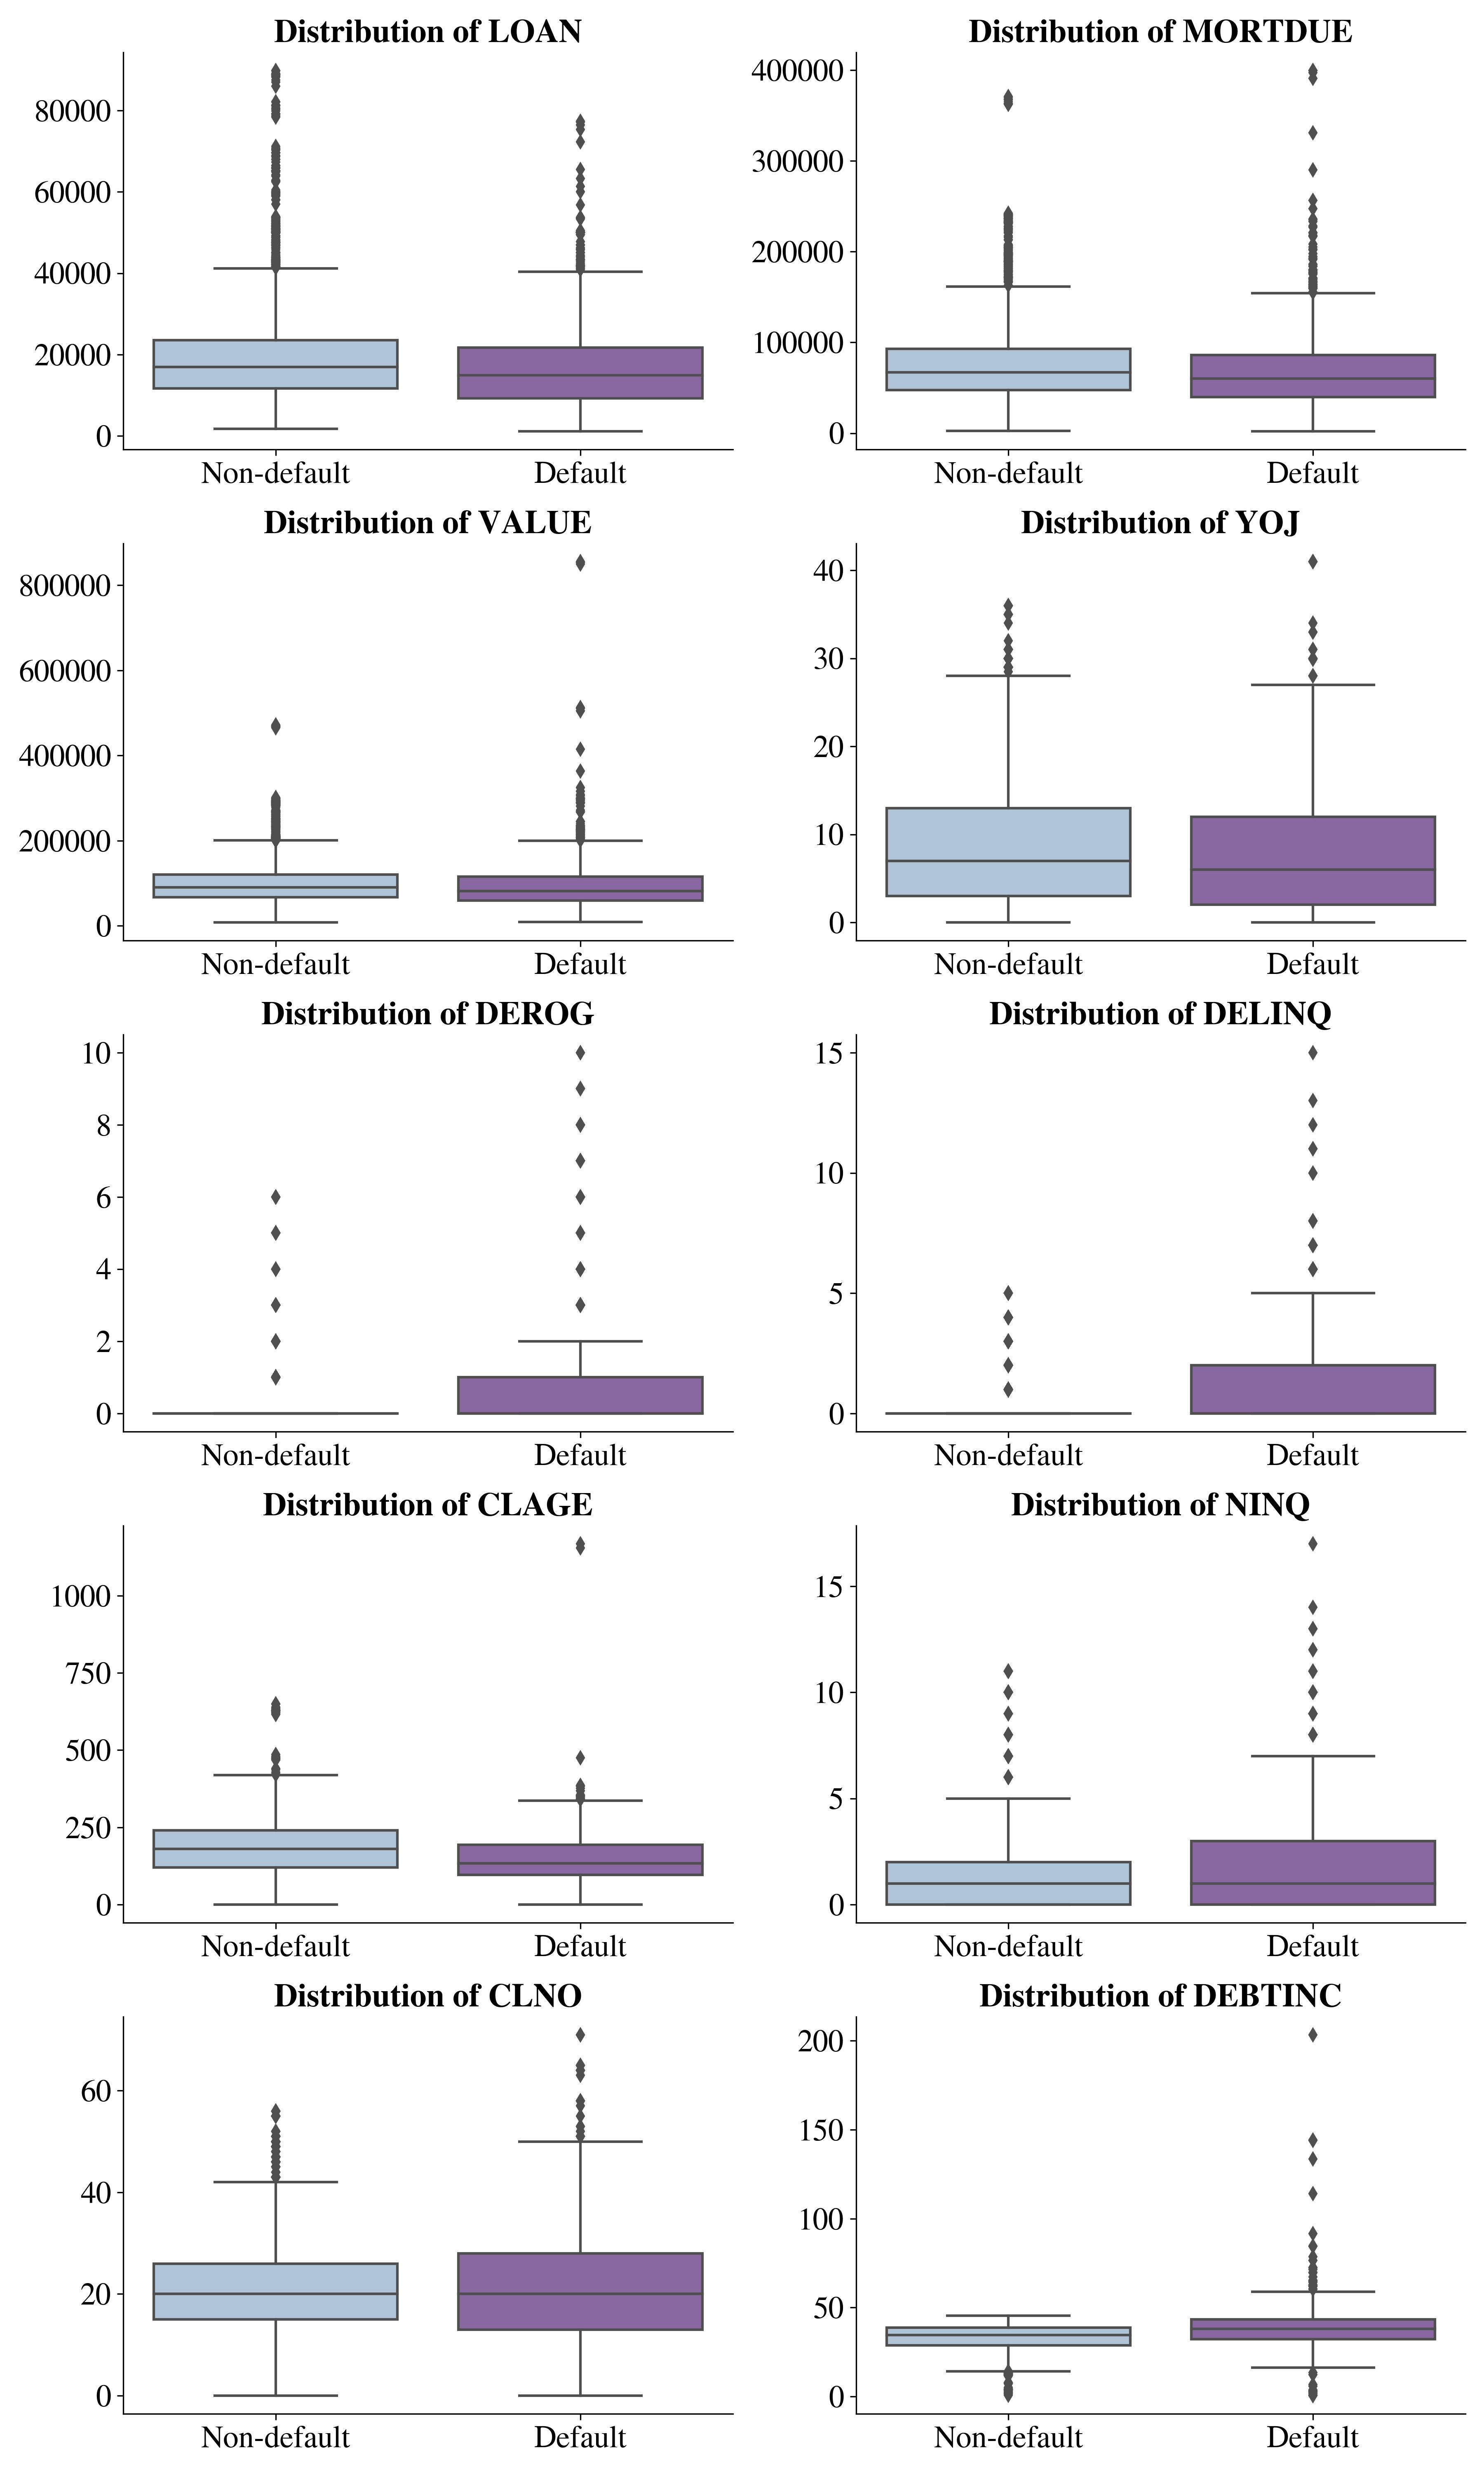
\includegraphics[width=140mm]{Figures/Numeric_Features_Distribution_Boxplots.jpg}
\centering{\begin{source}Author's results in Python\end{source}}\vspace{-1em}
\end{figure}

Due to the fact that the boxplots do not capture the missing values occurred in given features, it is also important to inspect the numbers and proportions of missing values in each feature, conditional on the default status.
As can be seen in \autoref{tab:nacont-table}, $n_0$ refers to the number of missing values in given feature for non-default cases, $n_1$ refers to the number of missing values in given feature for default cases.
$N_0$ and $N_1$ refer to the total number non--default cases and default cases respectively, therefore $n_0/N_0$ refers to the proportion of missing values in given feature for non-default cases, and $n_1/N_1$ refers to the proportion of missing values in given feature for default cases.

Pertaining to the feature \texttt{DEBTINC}, we can observe a significant difference in the number of missing values between the default and non-default cases. Out of all defaulted loans, 66.11 \% had missing debt--to--income ratio, whereas only 10.08 \% out of all non-defaulted loans had missing debt--to--income ratio.
Therefore, there could be a strong association between the missing debt--to--income ratio and the default.

Similarly, the table depicts a significant difference with respect to \texttt{VALUE} as 0.15 \% had missing collateral property value out of all non--defaulted loan, and 8.92 \% defaulted loans had missing collateral property value.
It can be inferred that loan applicants who withhold information on their collateral property value or debt-to-income ratio are more likely to default on their loans.
This may be due to negative information that they are trying to conceal, such as an excessively high debt or low income, or a low collateral property value.
Such associations are further investigated in \autoref{subsubsec:target-na-ass}.


\begin{table}[H]
\small
\setlength{\tabcolsep}{8pt}
\renewcommand{\arraystretch}{1.3}
% define a new column type 'L' for left alignment
\newcolumntype{R}[1]{>{\raggedleft\arraybackslash}p{#1}} % define a new column type 'R' for right alignment
\begin{center}
\caption[Numeric features NA's Summary]{Numeric features NA's Summary}\label{tab:nacont-table}
\begin{tabular}{l R{1cm}R{1cm}|R{1.5cm}R{1.5cm}}
    \toprule
    \textbf{Feature} & \textbf{$n_0$} & \textbf{$n_1$} & \textbf{$n_0/N_0$} & \textbf{$n_1/N_1$} \\
    \midrule
    \hline
    LOAN & 0 & 0 & 0 \% & 0 \% \\

    MORTDUE & 412 & 106 & 8.64 \% & 8.92 \% \\

    VALUE & 7 & 105 & 0.15 \% & 8.83 \% \\

    YOJ & 450 & 65 & 9.43 \% & 5.47 \% \\

    DEROG & 621 & 87 & 13.02 \% & 7.32 \% \\

    DELINQ & 508 & 72 & 10.65 \% & 6.06 \% \\

    CLAGE & 230 & 78 & 4.82 \% & 6.56 \% \\

    NINQ & 435 & 75 & 9.12 \% & 6.31 \% \\

    CLNO & 169 & 53 & 3.54 \% & 4.46 \% \\

    DEBTINC & 481 & 786 & 10.08 \% & 66.11 \% \\ \hline
    \bottomrule
\end{tabular}
\end{center}
\begin{center}
\source{Author's results in Python}
\end{center}
\end{table}
\subsubsection{Categorical Features' Distribution}
\label{subsubsec:catdist}

Regarding the distribution of categorical features, the data set includes 2 nominal features, namely \texttt{REASON} and \texttt{JOB}.
The conditional distribution of categorical features on the default status is visualized using barplots in \autoref{fig:catdist}.
The plot indicates that most loan applicants applied for debt consolidation, while most job occupancies were labeled as \texttt{Other}.

With respect to the default status, there appears to be no significant difference between the default and non-default cases in terms of the relative distribution of the \texttt{REASON} feature.
However, a slight difference is observed between the default and non-default cases in terms of the relative distribution of the \texttt{JOB} feature.
Specifically, the categories \texttt{Office}, \texttt{ProfExe}, and \texttt{N/A} exhibit a relatively higher proportion of non-default cases than default cases.
Hence, a moderate association between the \texttt{JOB} feature and the default status is possible, as further investigated in \autoref{subsubsec:target-cat-ass}.


\begin{figure}[H]
\centering
\caption{Conditional Distribution of Categorical Features}\vspace{0.5em}
\label{fig:catdist}
\includegraphics[width=140mm]{Figures/Categorical_Features_Distribution.jpg}
\centering{\begin{source}Author's results in Python\end{source}}\vspace{-1em}
\end{figure}
\subsection{Association Analysis}
In this subsection, we aim to examine potential relationships between the variables by analyzing their associations. Firstly, we investigate the association between the default status and the features. Subsequently, we explore the association among the features themselves.

\subsubsection{Association between default status and numeric features}
\label{subsubsec:target-num-ass}

To measure the association between the target variable and the numeric features, we use the Point-Biserial correlation coefficient, which is the Pearson's product moment correlation coefficient between a continuous variable and a dichotomous variable \citep{kornbrot2014point}.
This coefficient ranges from -1 to +1 and can be used to assess the strength and direction of the relationship between a continuous variable and a binary variable.
The formula for computing this coefficient is as follows:

\begin{equation}\label{eq}
r_{pb,X} =  \frac{\mu \left( X | Y=1 \right) -\mu \left( X | Y=0 \right)}{\sigma_{X}}\sqrt{\frac{N\left(Y=1\right) \times N\left(Y=0\right)}{N \left(N - 1 \right)}}
\end{equation}

Here, $\mu \left( X | Y=1 \right)$ and $\mu \left( X | Y=0 \right)$ represent the means of the given numeric feature $X$ conditional on the default status and non-default status, respectively, while $\sigma_{X}$ denotes the standard deviation of $X$.
The values of $N\left(Y=1\right)$ and $N\left(Y=0\right)$ indicate the number of observations with default status and non-default status, respectively, and $N$ represents the total number of observations within the feature $X$.


The following \autoref{tab:pointbi} displays the computed Point-Biserial coefficient for each numeric feature with respect to the default status, along with its statistical significance.
The results show that features such as \texttt{DEROG}, \texttt{DELINQ}, and \texttt{DEBTINC} are moderately and positively associated with the default status at the 1\% statistical significance level.
These findings support the observations made in \autoref{subsubsec:numdist} regarding the positive associations of these features with the default status. It can be inferred that these features may serve as important predictors in the model.

\begin{table}[H]
    \small
    \setlength{\tabcolsep}{8pt}
    \renewcommand{\arraystretch}{1.3}
    \centering
        \caption[Point--Biserial Correlation - Numeric Features vs. Default]{Point--Biserial Correlation - Numeric Features vs. Default}\label{tab:pointbi}
        \begin{tabular}{@{} l r @{\hspace{1cm}} l @{}}
    \toprule
    \textbf{Feature} & \textbf{Coefficient} & \textbf{Significance}\\
    \midrule
    \hline

    LOAN & -0.075  & ***\\

    MORTDUE & -0.048  & ***\\

    VALUE & -0.030  & ** \\
    
    YOJ & -0.060  & *** \\

    DEROG & 0.276 & *** \\

    DELINQ & 0.354 & *** \\
    
    CLAGE & -0.170 & *** \\

    NINQ & 0.175 & *** \\

    CLNO & -0.004 & \\

    DEBTINC & 0.200 & *** \\
    \hline
    \bottomrule
    \end{tabular}
    \vspace{0.35em}


        \centering\footnotesize{$^{*}$: $p<0.10$, $^{**}$: $p<0.05$, $^{***}$: $p<0.01$}\vspace{0.7em}

        \centering{\begin{source}Author's results in Python\end{source}}\vspace{-1em}

\end{table}

\subsubsection{Association between default status and categorical features}
\label{subsubsec:target-cat-ass}

In order to measure the strength of the relationship between the dichotomous default status and categorical variables, we employ Cramer's V, which ranges from 0 to 1 and is defined as:


\begin{equation}\label{eq}
    CV_{X} = \sqrt{\frac{\chi^{2}}{N\left(k-1\right)}}
\end{equation}


As noted in \autoref{subsubsec:catdist}, the association between the default status and \texttt{REASON} is weak, as evidenced by the Cramer's V value being close to zero.
Conversely, the association between the default status and \texttt{JOB} is slightly stronger, as the categories \texttt{Office}, \texttt{ProfExe}, and \texttt{N/A} exhibit a higher proportion of non-default cases than default cases.
Both \texttt{REASON}'s and \texttt{JOB}'s associations with default status are statistically significant at the 1\% significance level.

While statistical significance is important, it does not necessarily indicate that a feature is a strong predictor of the target variable.
Ultimately, the usefulness of a feature in predicting the target variable is determined by the performance metrics of the model.

    \begin{table}[H]
        \small
        \setlength{\tabcolsep}{8pt}
        \renewcommand{\arraystretch}{1.3}
        \centering
            \caption[Cramer's V Association - Categorical Features vs. Default]{Cramer's V Association - Categorical Features vs. Default}\label{tab:cramer-v}
            \begin{tabular}{@{} l r @{\hspace{1cm}} l @{}}
        \toprule
        \textbf{Feature} & \textbf{Coefficient} & \textbf{Significance}\\
        \midrule
        \hline
        REASON & 0.038  & ***\\
        JOB & 0.120  & ***\\
        \hline
        \bottomrule
    \end{tabular}
    \vspace{0.35em}


        \centering\footnotesize{$^{*}$: $p<0.10$, $^{**}$: $p<0.05$, $^{***}$: $p<0.01$}\vspace{0.7em}

        \centering{\begin{source}Author's results in Python\end{source}}\vspace{-1em}
\end{table}

\subsubsection{Association between default status and missing values}
\label{subsubsec:target-na-ass}

Given that the loan data set contains missing values, it is necessary to examine whether the missingness is associated with the default status. One possible approach is to encode the feature with missing values as a binary variable, where 1 indicates the presence of a missing value and 0 otherwise.

To quantify the strength of association between the two binary variables, the Phi coefficient is used, which is defined as:

\begin{equation}\label{eq}
\phi_{X} = \sqrt{\frac{\chi^{2}}{n}}
\end{equation}

In line with the finding regarding the \texttt{DEBTINC} and \texttt{VALUE} in \autoref{subsubsec:numdist}, there is a strong and statistically significant association between the missing debt-to-income ratio and default status, and a moderate and statistically significant association between the missing collateral property value and default status, as shown in \autoref{tab:phi-target}.
Therefore, we can anticipate that these features will be crucial indicators in default prediction. Further details on feature selection are presented in \autoref{subsec:feature-selection}.
\begin{table}[H]
    \small
    \setlength{\tabcolsep}{8pt}
    \renewcommand{\arraystretch}{1.3}
    \centering
        \caption[Phi Correlation Coefficient - NA's vs. Default]{Phi Correlation Coefficient - NA's vs. Default}\label{tab:phi-target}
        \begin{tabular}{@{} l r @{\hspace{1cm}} l @{}}
    \toprule
    \textbf{Feature} & \textbf{Coefficient} & \textbf{Significance}\\
    \midrule
    \hline
    LOAN & 0.000  & \\

    MORTDUE & 0.003  & \\
 
    VALUE & 0.254  & *** \\

    REASON & 0.004 & \\

    JOB & 0.064 & *** \\

    YOJ & 0.056  & *** \\

    DEROG & 0.070 & *** \\

    DELINQ & 0.061 & *** \\

    CLAGE & 0.030 & ** \\

    NINQ & 0.039 & *** \\

    CLNO & 0.018 & \\

    DEBTINC & 0.547 & *** \\
    \hline
    \bottomrule
    \end{tabular}
    \vspace{0.35em}


        \centering\footnotesize{$^{*}$: $p<0.10$, $^{**}$: $p<0.05$, $^{***}$: $p<0.01$}\vspace{0.7em}

        \centering{\begin{source}Author's results in Python\end{source}}\vspace{-1em}
\end{table}

\subsubsection{Missing Values Association}
Additionally, it is imperative to investigate the relationship between missing values and default status, as well as the interrelationship between the missing values themselves.
A common approach to identifying patterns of missing data in a data set is through the use of a dendrogram, which clusters variables hierarchically based on the occurrence of missing values.
This method groups variables into clusters based on the similarity of their missing value patterns, such that variables with comparable patterns of missingness are clustered together.
Conversely, variables with dissimilar patterns of missingness are placed in separate clusters.
The dendrogram is constructed by merging the two closest clusters iteratively until all variables are in the same cluster.
The distance between the clusters at each step of the merging process is shown on the y-axis of the dendrogram, and the order in which the variables are merged is displayed on the x-axis.

In \autoref{fig:dendrogram}, the hierarchical clustering of the data set's variables is illustrated, excluding the default status and requested loan amount feature \texttt{LOAN}, as these variables do not contain any missing values.
As depicted in the dendrogram, the \texttt{CLNO} and \texttt{CLAGE} features have the most similar patterns of missing values occurrences.
Therefore, it can be inferred that a significant number of loan applicants tend to omit information regarding their number of credit lines (\texttt{CLNO}) and the age of their most recent credit line (\texttt{CLAGE}) when submitting their loan applications.

\begin{figure}[H]
    \centering
    \caption{Nullity Dendrogram}\vspace{0.5em}
    \label{fig:dendrogram}
    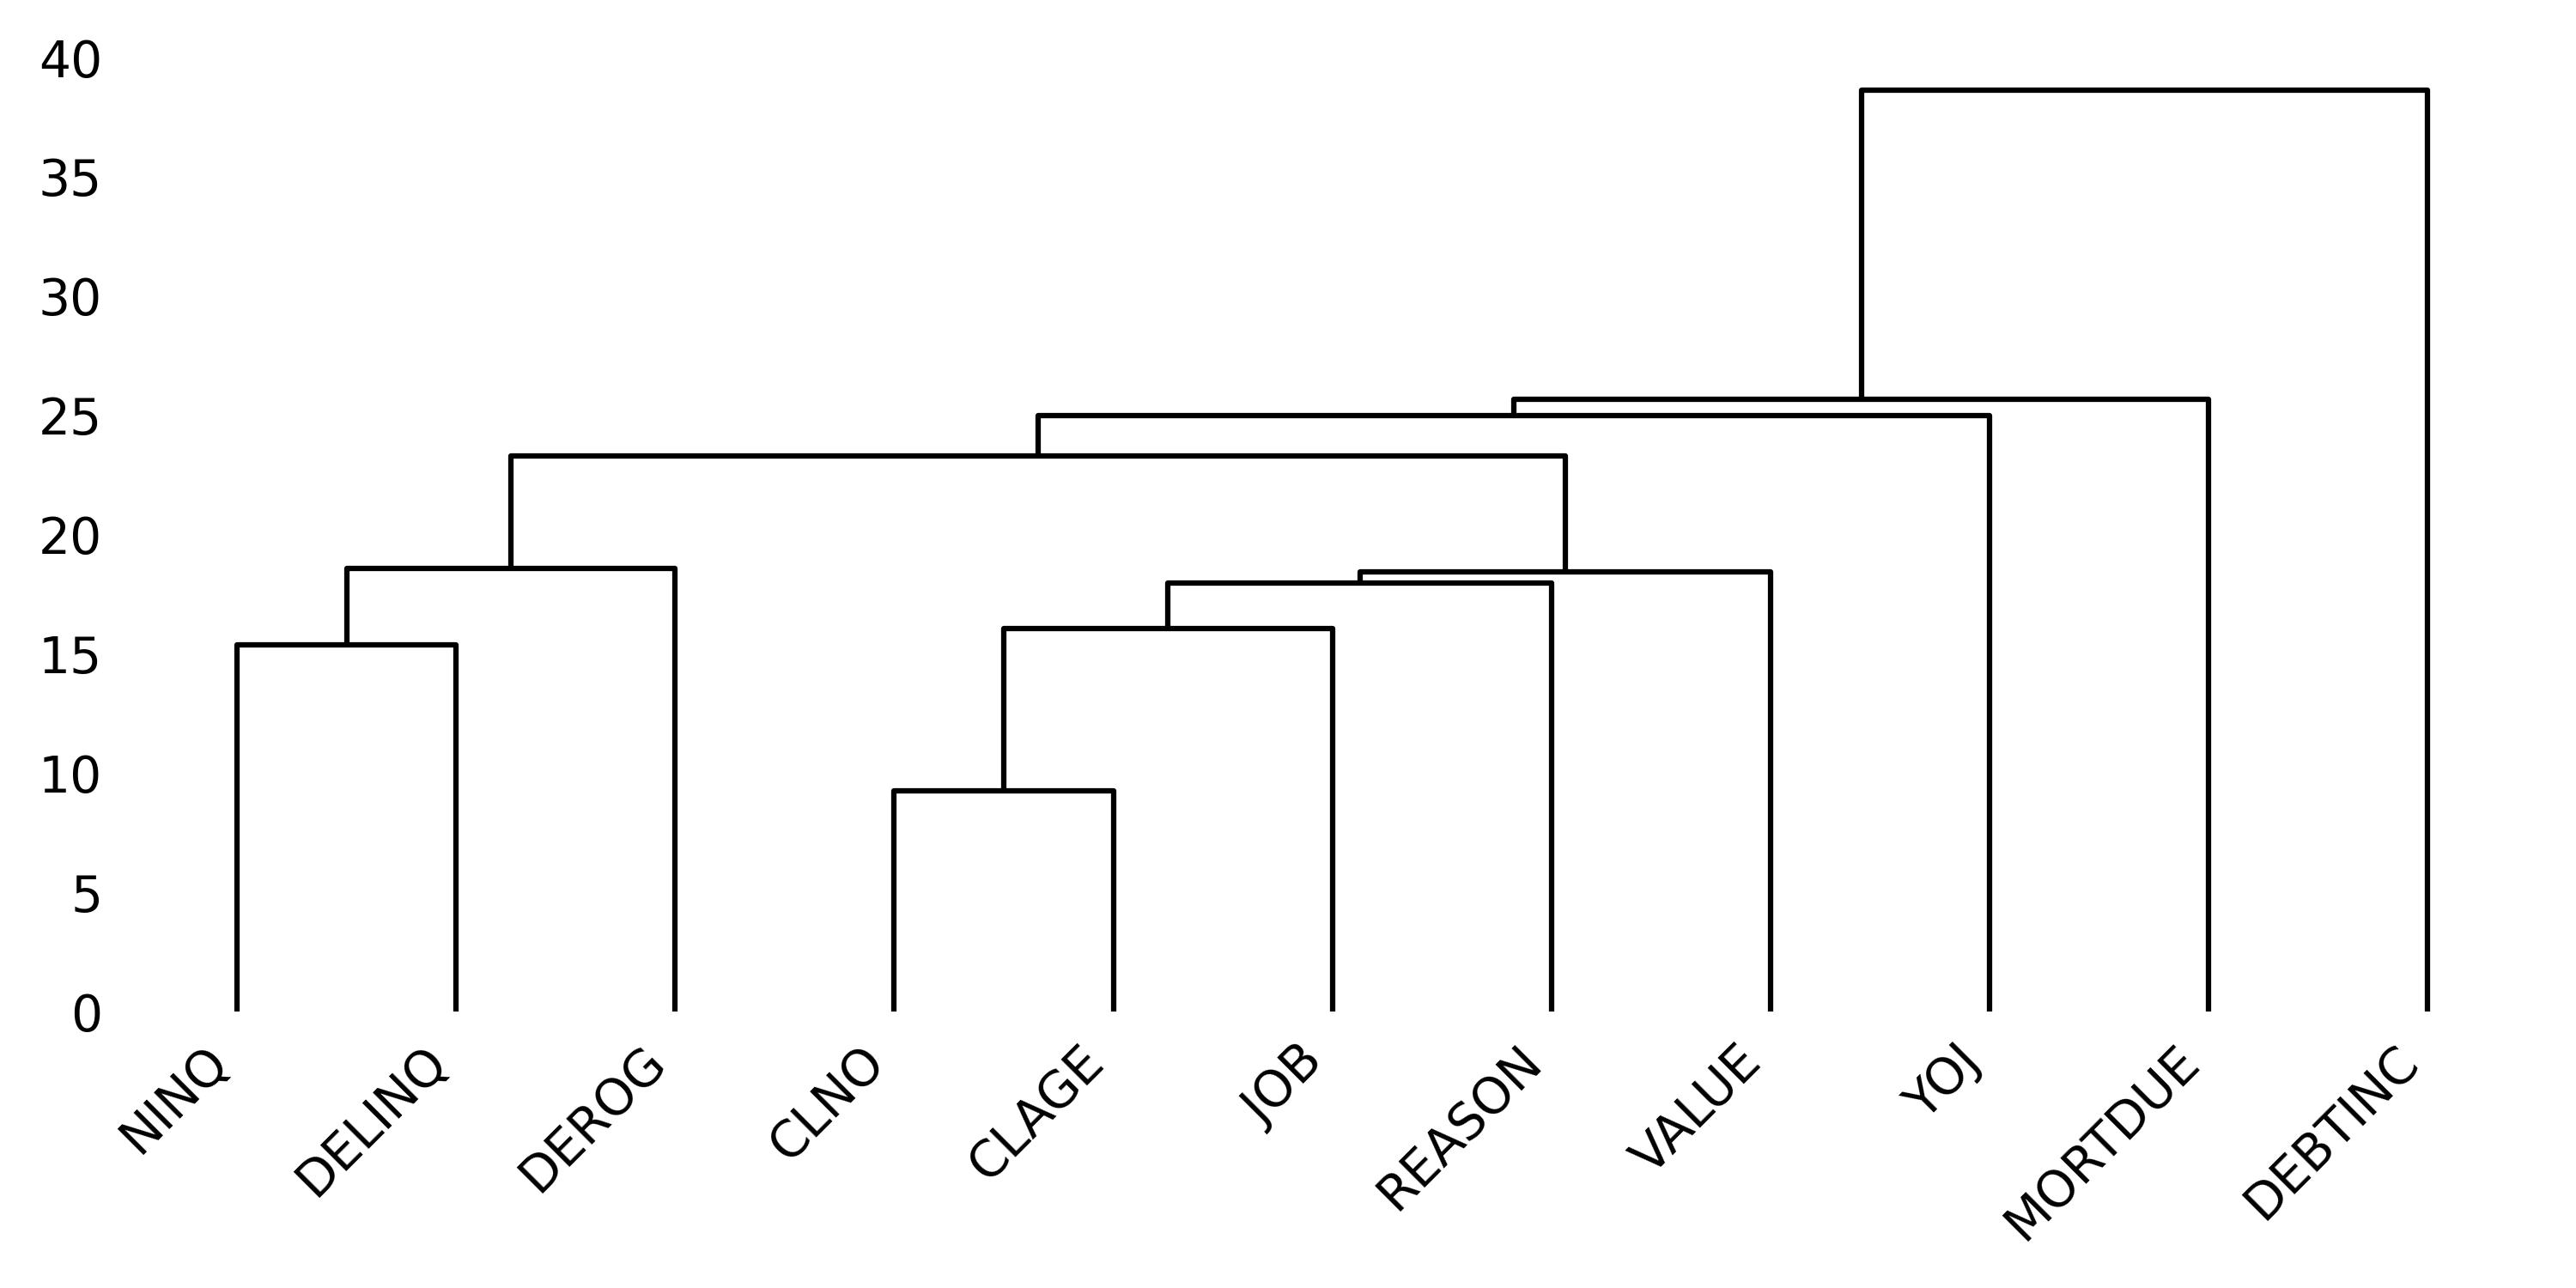
\includegraphics[width=140mm]{Figures/NA_Dendrogram.jpg}
    \centering{\begin{source}Author's results in Python\end{source}}\vspace{-1em}
\end{figure}

\subsubsection{Multicolinearity Analysis}

To quantify the association between the numerical features, Pearson correlation coefficient is often used.
However, it is highly sensitive to outliers and makes assumptions regarding the normal distribution and linear relationship between variables.
Consequently, Spearman correlation coefficient is utilized as an alternative, as it is a non-parametric measure that does not make any assumptions regarding the distribution of variables or the linearity of their relationship.
The Spearman correlation coefficient is defined as follows:

\begin{equation}\label{eq}
\rho_{spearman} = 1 - \frac{6 \sum_{i=1}^{n} d_{i}^{2}}{n \left(n^{2}-1\right)}
\end{equation}


In the \autoref{fig:spearmancorr}, we can observe a very strong correlation between the \texttt{MORTDUE} and \texttt{VALUE} features. Such multicolinearity can cause problem in predictions na model's overfitting. Therefore, a feature selection is recommended - such selection is further described in \autoref{subsec:feature-selection}.

\begin{figure}[H]
    \centering
    \caption{Spearman Correlation Matrix}\vspace{0.5em}
    \label{fig:spearmancorr}\
    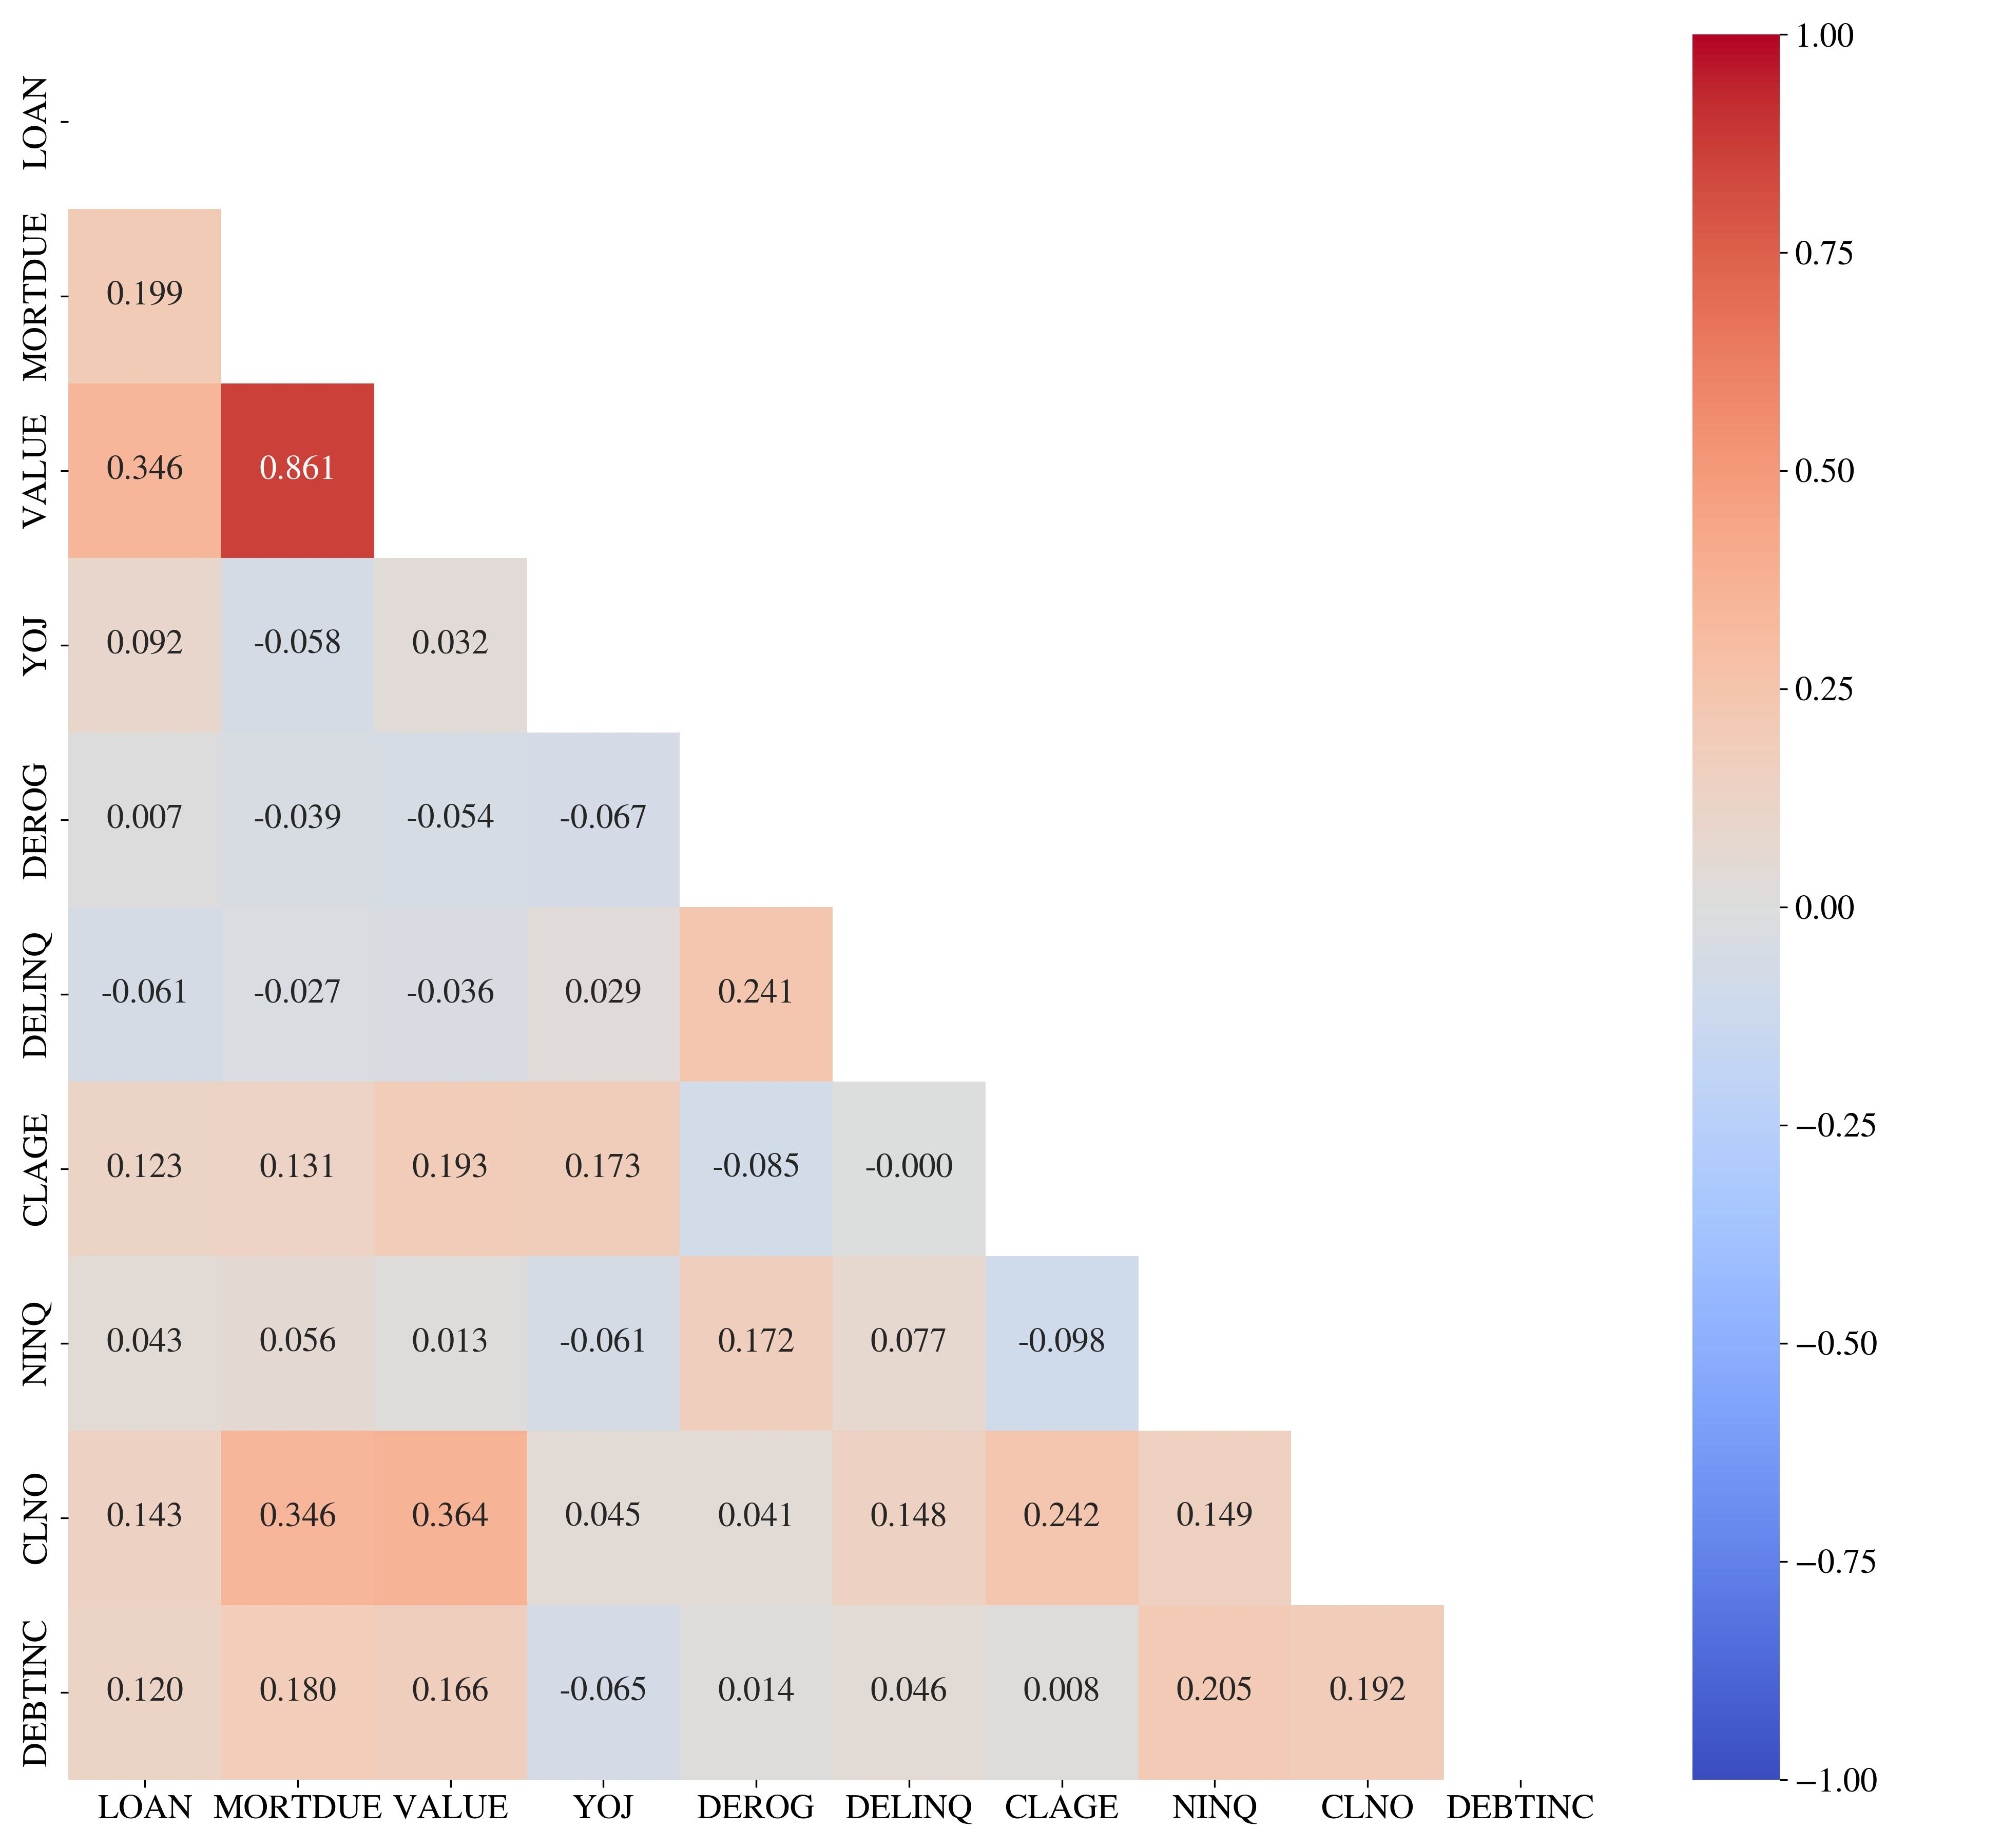
\includegraphics[width=150mm]{Figures/Spearman_Correlation_Matrix_Numeric_Features.jpg}
    \centering{\begin{source}Author's results in Python\end{source}}\vspace{-1em}
\end{figure}

\newpage
\section{Data Preprocessing}
In this section, the process of preprocessing data is described as the crucial step in the machine learning modelling. Particularly, the the process of dividing data for various tasks, oversampling due to the imbalanced class issue, discretization of features and Weight--of--Eveidence transformation are further discussed and described.

\subsection{Data Split and ADASYN Oversampling}
\label{subsec:data-split-ADASYN}

To ensure appropriate model training and unbiased evaluation, it is necessary to split data into separate sets for various purposes. Specifically, the data set is split into three sets: (1) training set for training the model, perform feature selection or hyperparameter tuning, (2) validation for hyperparameter tuning, and (3) test set for assess the model performance on the unseen data \citep{subasi2020practical}.
In this thesis, the data is plit into training, validation and test sets in ratio of 70:15:15, which ensures sufficient amount of data for training, hence the model would be able to generalize well, while keeping the validation and test sets large enough to provide reliable evaluation of the model's performance.

The data is split using stratified split to preserve the default status distribution, which is highly imbalanced.
Stratification ensures that the distribution of defaults and non-defaults remains the same across all sets, thereby avoiding overfitting and data leakage. Using stratification, each set had 80 \% non-defaults and 20 \% defaults. This method enables accurate prediction since the model is trained and evaluated on the same population \citep{igareta2021strat}.
However, stratification alone may not be sufficient for dealing with imbalanced classes. Therefore, ADASYN oversampling is performed as described in \autoref{sec:adasyntheory}. Note that ADASYN oversampling is performed on the training set only after the split to avoid data leakage and biased evaluation.

In Python, the data are divided and oversampled using a custom function \lstinline{data_split()}.
This function first employs the \lstinline{train_test_split()} function from the \lstinline{scikit-learn} module to split the data into training, validation, and test sets with a stratification technique.
Next, the \lstinline{ADASYN()} class from the \lstinline{imblearn} module is used to oversample the training set. This is achieved by generating synthetic instances of the minority class based on the five nearest neighbors and Euclidean distance.

However, the \lstinline{ADASYN()} class from \lstinline{imblearn} is not designed to handle missing values or categorical features encoded as character. To overcome this limitation, the following approach is taken:
\begin{enumerate}\setlength\itemsep{0em} 
\item Separate the categorical and numeric features;
\item Impute the missing values with arbitrary values:
\begin{itemize}
\item Categorical features: string \lstinline{'N/A'};
\item Numeric features: number \lstinline{99999999999999} - such value is chosen since it is highly unlikely to be present in the data set.
\end{itemize}
\item Convert the categorical features into dummy variables;
\item Join the numeric features with the dummy variables;
\item Perform the oversampling on the joined data set;
\item Convert the dummy variables back into categorical features;
\item Retrieve back the missing values:
\begin{itemize}
\item Categorical features: replace string \lstinline{'N/A'} with \lstinline{np.nan};
\item Numeric features: for each feature $X$ if its value exceeds the its original maximum value, then replace it with \lstinline{np.nan};
\end{itemize}
\end{enumerate}


The following \autoref{tab:split} shows the default distribution of the individual sets before and after oversampling. The default distribution in training set after ADASYN oversampling is balanced, while the default distribution remains the same across the validation and test sets, which is desirable due to stratification.
\begin{table}[H]
\small
\setlength{\tabcolsep}{8pt}
\renewcommand{\arraystretch}{1.3}
\centering
    \caption[Data Split Summary]{Data Split Summary}\label{tab:split}
    \begin{tabular}{lrrr}
\toprule
\textbf{Set} & \textbf{\# instances} & \textbf{\% defaults} & \textbf{\% non--defaults}\\
\midrule
\hline
Training & 4,171  & 19.95 \% & 80.05 \% \\
Training (oversampled) & 6,437 &  48.13 \% & 51.87 \% \\

Validation & 895 &  20.00 \% & 80.00 \% \\

Test & 894 &  20.00 \% & 80.00 \% \\
\hline
\bottomrule
\end{tabular}
\vspace{0.7em}

\centering{\begin{source}Author's results in Python\end{source}}\vspace{-1em}
\end{table}

Since ADASYN increases the sample size by generating, i.e., adding new instances into the sample, it may have an impact on the distribution of the features.
After the inspection in Python, it have no significant impact on the numeric features as the distributions before and after ADASYN oversampling do not differ that much.
However, pertaining to the categorical features, a significant impact of ADASYN oversampling can be observed as can be seen in  \autoref{tab:adasynimpact} and \autoref{fig:adasynimpact}, respectively, which depict the distribution of categorical features on the subsample of default cases within the training set, particularly distribution before and after the oversampling.
As such, $n_B$ and $n_A$ refer to the number of default cases within given category before and after oversampling, respectively, $N_B$ and $N_A$ represents the total number of default cases before and after oversampling, respectively.

Within the \texttt{REASON} feature, we can observe a significant increase the proportion of defaulted clients who applied for a loan due to the debt consolidation (\texttt{DebtCon}) among all the defaulters after an oversampling - particularly, the ratio has increased by 12.20 percentage points.
On the other hand, the proportion of defaulted clients who applied for a loan due to the home improvement (\texttt{HomeImp}) has decreased by 9.69 percentage points, indicating lower distribution of such clients in the oversampled set.
Regarding the \texttt{JOB} feature, we can observe a substantial increase in the proportion in the of defaulted managers (\texttt{Mgr}) among all the defaulters after oversampling by 38.75 percentage points.
On the other hand, the proportion of defaulted clients who are labelled as \texttt{Others} has decreased by 17.15 percentage points.

\begin{table}[H]
    \small
    \setlength{\tabcolsep}{8pt}
    \renewcommand{\arraystretch}{1.3}
    \centering
    \caption[ADASYN Impact on Categorical Features' Distribution]{ADASYN Impact on Categorical Features' Distribution}\label{tab:adasynimpact}
    \begin{tabular}{|ll|rr|rr|r|}
    
        \hline
    \textbf{Features} & \textbf{Category} & \textbf{$n_{B}$} & \textbf{$n_{A}$} & \textbf{$n_{B} / N_{B}$} & \textbf{$n_{A} / N_{A}$} & \textbf{Diff.} \\ 
    \midrule
    \midrule
    REASON & DebtCon & 528 & 2,344 & 63.46 \% & 75.66 \% & 12.20 p.p. \\ 
    REASON & HomeImp & 274 & 720 & 32.93 \% & 23.24 \% & -9.69 p.p. \\
    REASON & N/A & 30 & 34 & 3.61 \% & 1.10 \% & -2.51 p.p. \\
    \hline
    JOB & Mgr & 124 & 1,662 & 14.9 \% & 53.65 \% & 38.75 p.p. \\ 
    JOB & Other & 396 & 943 & 47.6 \% & 30.44 \% & -17.16 p.p. \\ 
    JOB & ProfExe & 142 & 272 & 17.07 \% & 8.78 \% & -8.29 p.p. \\ 
    JOB & Office & 85 & 104 & 10.22 \% & 3.36 \% & -6.86 p.p. \\ 
    JOB & Self & 39 & 58 & 4.69 \% & 1.87 \% & -2.82 p.p. \\
    JOB & Sales & 29 & 36 & 3.49 \% & 1.16 \% & -2.33 p.p. \\ 
    JOB & N/A & 17 & 23 & 2.04 \% & 0.74 \% & -1.30 p.p. \\ 
    \hline
    \bottomrule
    \end{tabular}
    \vspace{0.7em}
    
    \centering{\begin{source}Author's results in Python\end{source}}\vspace{-1em}
\end{table}

Such findings regarding the significant increases in the proportion of default cases regarding the \texttt{DebtCon} and \texttt{Mgr} categories are given to the nature of ADASYN oversampling.
As explained before, ADASYN generates more synthetic default class instances in the neighborhood of such default instances, which are hard--to--learn for ADASYN.
In other words, ADASYN creates more default instances for such default instances where the density of the non--default class is relatively high in given default instance's neighborhood.
Therefore, default instances which either are managers or applied for a loan due to the debt consolidation are difficult--to--learn for ADASYN, thus ADASYN replicates more instances with such characteristics, hence this results in a higher proportion of default cases in the oversampled set for such category.


\begin{figure}[H]
    \centering
    \caption{ADASYN Impact of Categorical Features' Distribution}\vspace{0.5em}
    \label{fig:adasynimpact}\
    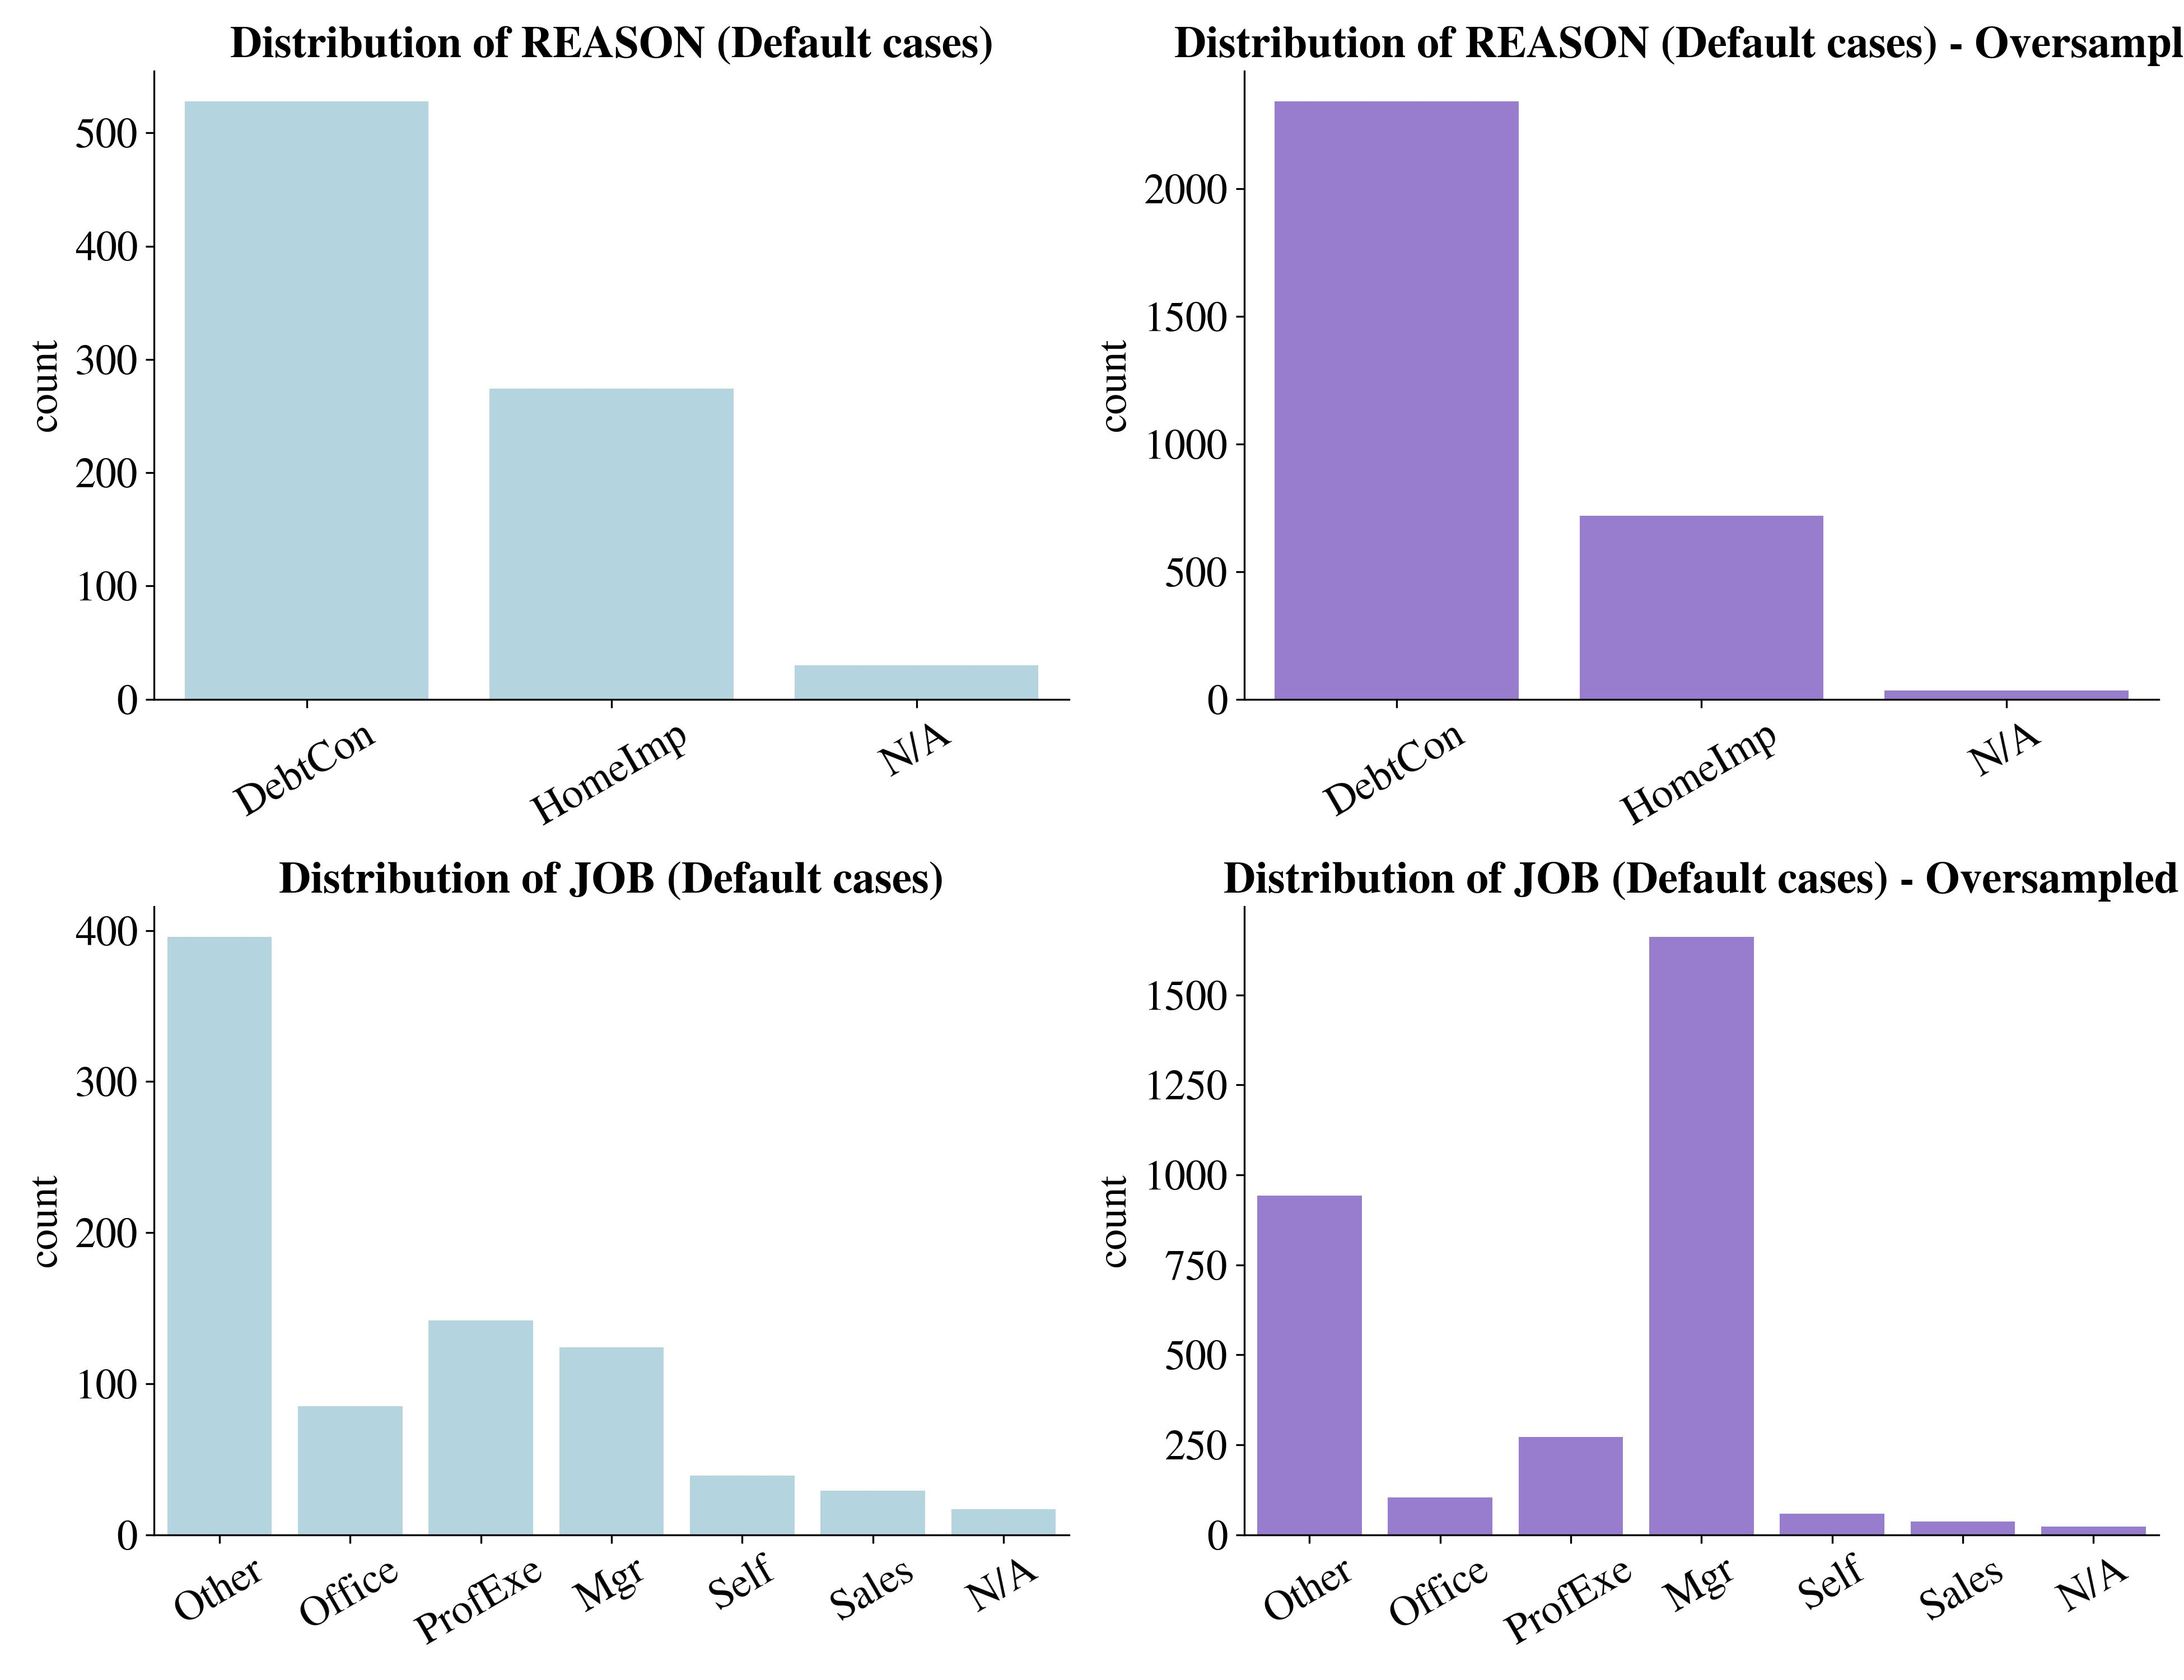
\includegraphics[width=140mm]{Figures/Categorical_Features_Distribution_OS_Default.jpg}
    \centering{\begin{source}Author's results in Python\end{source}}\vspace{-1em}
\end{figure}



\newpage
\subsection{Optimal Binning and Weight--of--Evidence}
\label{subsec:prep-optbinning}
As already described in \autoref{sec:optbinningtheory}, the optimal binning is employed as a data preprocessing step in this thesis.
Particularly, we employ \lstinline{BinningProcess} class from the \lstinline{optbinning} module in Python - such class optimally discretizes the continuous features into interval bins and optimally groups categorical features' categories into sub-group categories with respect to the target variable while maximizing Information Value, and afterwards such bins are encoded using WoE \citep{navas2020optimal}. Besides discretizing and grouping, it also creates special bins for capturing missing values.


In this thesis, this data preprocessing step is wrapped into a custom function \lstinline{woe_binning()} in Python.
First, the  \lstinline{BinningProcess} class is fitted on the training set only in order to avoid data leakage, while it learns the split points for binning, event rates, WoE coefficients etc., and afterwards, such fitted  \lstinline{BinningProcess} class is used to transform training, validation and test set.


The following \autoref{fig:woedist} depicts the distribution of WoE bins for each feature. It can be observed that binning captures either linear, non-linear, monotonic, or non-monotonic relationships between the default status and the numeric features in terms of WoE.
Regarding the \texttt{DELINQ} feature, a monotonic relationship can be observed, where the higher number of delinquent credit lines, the lower the WoE coefficient, indicating a larger distribution of defaults with respect to non-defaults in the given bin.
Thus, the higher the number of delinquent credit lines, the higher the likelihood of defaulting in terms of WoE.

A non-linear relationship can be observed with respect to the \texttt{YOJ} feature, where the WoE coefficient is positive for applicants who have recently started working at their new job (i.e., number of years at the present job is less than 1) and for applicants who have been working at their current job for a relatively long time (i.e., number of years at the present job is higher than 19).
Thus, applicants who have been working for a longer time have stable income and are more creditworthy and less likely to default.
Regarding applicants who have recently started working at their new job, it is possible that they are less likely to default since the \texttt{YOJ} feature does not capture the applicant's total number of years of work experience, but only the number of years at the present job.
Thus, in the given data set, applicants who have recently started working at their new job have a relatively higher total number of years of work experience, making them more creditworthy and less likely to default. On the other hand, for applicants who have been working at their present job between 1 and 19 years, the WoE coefficient is negative.
This relationship seems to be complex and can be influenced by other factors not present in the data set, such as the applicant's age, total number of years of work experience, education, etc.

As already mentioned numeric and categorical features contain a separate bin capturing missing values, which can be a useful indicator when training a model. This is evident in the \texttt{DEBTINC} feature, where the bin capturing missing values has the most negative WoE coefficient, indicating that there is a larger distribution of defaulters compared to non-defaulters.
This finding was already raised in \autoref{subsubsec:target-na-ass} in terms of the strong and statistically significant association between the default status and the missing values in \texttt{DEBTINC}.

Within the \texttt{JOB} feature, specifically regarding the \texttt{Mgr} category, we can observe the direct impact of ADASYN oversampling as already described by \autoref{tab:adasynimpact}.
Since ADASYN generated more default class instances for original default instances who are managers, this results in higher default rate within such job category, thus to the larger distribution of defaulters compared to non--defaulters, which is quantified in the negative WoE value.

\textbf{QUESTION FOR SUPERVISOR: should I also decsribe the WoE distribution for other features as well or is this sufficient?}


\begin{figure}[H]
\centering
\caption{WoE Bins Distribution}\vspace{0.5em}
\label{fig:woedist}
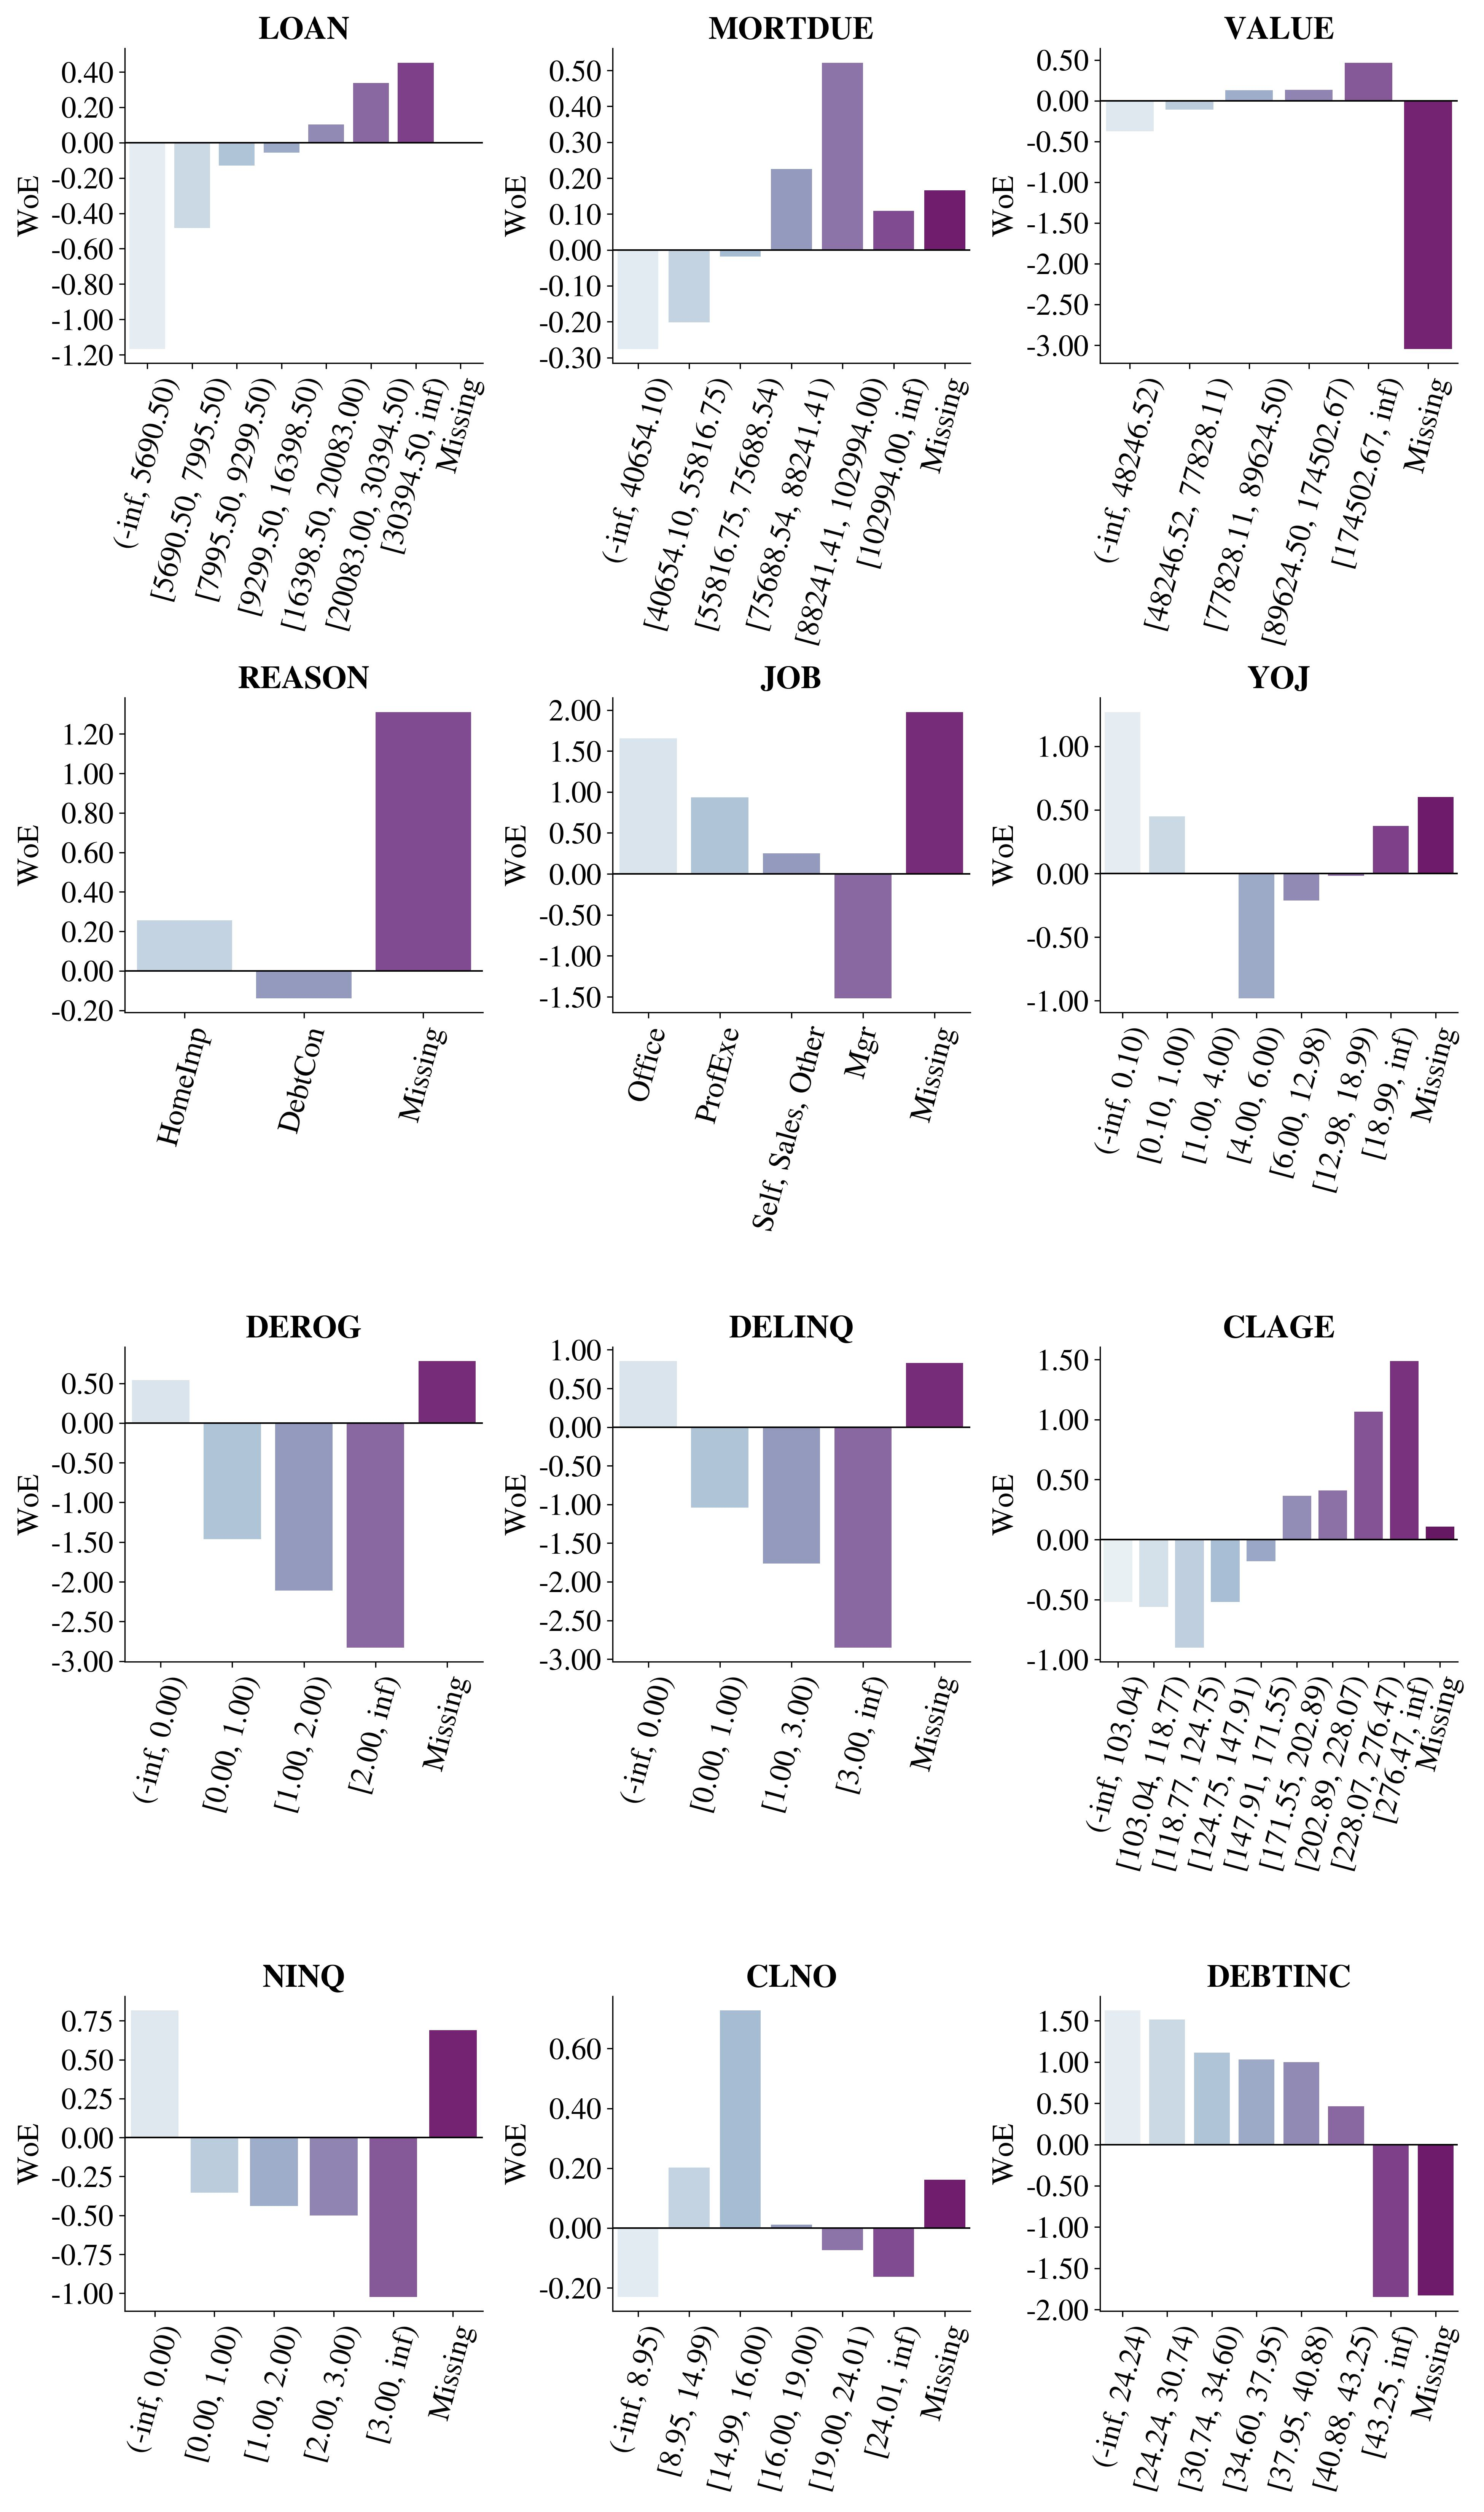
\includegraphics[width=140mm]{Figures/WoE_Distribution.jpg}
\centering{\begin{source}Author's results in Python\end{source}}\vspace{-1em}
\end{figure}

\newpage
\section{Modelling}
\label{sec:modelling}
Once the data are finally preprocessed, the next step regards the modelling part which includes hyperparameter tuning, feature selection, model selection and model building.

In Python, 8 different machine learning models from \lstinline{Scikit-learn} module are used for the default status prediction, which were already described in \autoref{sec:algorithms}, namely:
\begin{itemize}\setlength\itemsep{0em}
\item \textbf{Logistic Regression} - \lstinline{LogisticRegression()}
\item \textbf{Decision Tree} - \lstinline{DecisionTreeClassifier()}
\item \textbf{Gaussian Naive Bayes} - \lstinline{GaussianNB()}
\item \textbf{K-Nearest Neighbors} - \lstinline{KNeighborsClassifier()}
\item \textbf{Random Forest} - \lstinline{RandomForestClassifier()}
\item \textbf{Gradient Boosting} - \lstinline{GradientBoostingClassifier()}
\item \textbf{Support Vector Machine} - \lstinline{SVC()}
\item \textbf{Multi--Layer Percepton} (\textit{Neural Network}) - \lstinline{MLPClassifier()}
\begin{itemize}\setlength\itemsep{0em}
\item Henceforth, we will refer to Neural Network as \textbf{MLP}.
\end{itemize}
\end{itemize}

\subsection{Hyperparameter Bayesian Optimization}
In this thesis, hyperparameter tuning of models is performed using Bayesian Optimization as described in \autoref{sec:bayesoptheory}.
In Python, a custom function, \lstinline{bayesian_optimization()}, is implemented to perform hyperparameter tuning using Bayesian Optimization.
This function utilizes \lstinline{BayesSearchCV} class from the \lstinline{Scikit-optimize} module, with a 10-fold stratified cross-validation scheme and 50 iterations, while maximizing the F1 score. As a surrogate function, Gaussian Process is used \citep{scikit-opt}.
The use of \lstinline{BayesSearchCV} with stratified cross-validation in the hyperparameter tuning process provides a robust and reliable approach to selecting the optimal hyperparameters for the model, while the incorporation of Bayesian Optimization enables the efficient exploration of the hyperparameter space.
By maximizing the F1 score, the hyperparameters selected through this process will result in a model with improved performance. Note, that the hyperparameter tuning is performed solely on training set in order to preserve the independence of the validation and test set, and avoid the information/data leakage as well.

For each model, the Bayesian Optimization algorithm performs 50 iterations while searching for the best hyperparameters values that maximize the F1 score. Within each iteration, a 10-fold stratified cross-validation is conducted to evaluate the model's cross--validation F1 score.
Moreover, for each model, we specify the hyperparameter space, i.e., particular hyperparameters to be tuned and their possible ranges which the hyperparameter can take. The ranges are specified using \lstinline{Integer} class to define interval of integers, \lstinline{Real} to define interval of float numbers, and \lstinline{Categorical} to define a list of possible (categorical) values.
Note that not all the available hyperparameters are tuned, but only the most relevants due to the time complexity of the Bayesian Optimization algorithm.
The definition of hyperparameter space for each model is described further in the following subsubsections.

\subsubsection{Logistic Regression}
The first hyperparameter \textbf{\texttt{Intercept}} allows to specify whether the intercept should be estimated or not.
$C$ is the regularization strength, and it is used to specify the regularization penalty, i.e., the hyperparameter \textbf{\texttt{Penalty}}.
If the penalty is set to $ElasticNet$, we can also tune $L1$ ratio, which refers to the $\alpha$ parameter in in \autoref{eq:elasticnet}
Moreover, the  \textbf{\texttt{Class weight}} hyperparameter is a hyperparameter which allows to assign higher importance to the minority class instances during the training process.

Furthermore, \textbf{\texttt{Solver}} hyperparameter is used to specify which optimization algorithm should be used to estimate the coefficients' values.
According to Hale \citep{hale2019dont}, Scikit-learn provides five solvers for Logistic Regression, namely \textit{lbfgs} (Limited-memory Broyden-Fletcher-Goldfarb-Shanno) which approximates the second derivative matrix updates with gradient evaluations, \textit{liblinear} (Library for Large Linear Classification) which uses coordinate descent algorithm, \textit{newton-cg},
\textit{sag} (Stochastic Average Gradient descent) as a variation of gradient descent and incremental aggregated gradient approaches using random sample of previous gradient values, and \textit{saga} as an extension of \textit{sag} which allows $L1$ regularization.
For more information, please refer to the Scikit-learn documentation regarding Logistic Regression \citep{scikit-lr}.
The last hyperparameter of Logistic Regression to tune in this thesis is the \textbf{\texttt{Intercept scaling}} which allows to scale the intercept.

\begin{table}[H]
\small
\setlength{\tabcolsep}{8pt}
\renewcommand{\arraystretch}{1.3}
\centering
    \caption[Logistic Regression - Hyperparameter Space]{Logistic Regression - Hyperparameter Space}\label{tab:lrspace}
    \begin{tabular}{ll}
\toprule
\textbf{Hyperparameter} & \textbf{Space}\\
\midrule
\hline
Intercept & True, False \\
$C$ factor & <$1\times10^{-6}$, 5>\\
Penalty & L1, L2, Elastic Net, None \\
Solver & lbfgs, liblinear, newton-cg, sag, saga \\
Class weight & None, balanced \\
L1 ratio & <0, 1> \\
Intercept scaling & True, False  \\
\hline
\bottomrule
\end{tabular}
\vspace{0.7em}

\centering{\begin{source}Author's results in Python\end{source}}\vspace{-1em}
\end{table}


\subsubsection{Decision Tree}
The first hyperparameter of Decision Tree is the \textbf{\texttt{Criterion}} which allows to specify the function to measure the quality of a split - either Gini or Entropy impurity function.
Another important hyperparameter is the \textbf{\texttt{Max depth}} which allows to specify the maximum depth of the tree.
The last hyperparameter is the \textbf{\texttt{Max features}} which allows to specify the number of features to consider when looking for the best split \citep{scikit-dt}.
Note, that \textbf{\texttt{Max features}} has a variable range of values depending on the number of features which is dependent on the number of features selected during feature selection (where the feature are iteratively selected and the model is trained and evaluated on each iteration).
\begin{table}[H]
\small
\setlength{\tabcolsep}{8pt}
\renewcommand{\arraystretch}{1.3}
\centering
    \caption[Decision Tree - Hyperparameter Space]{Decision Tree - Hyperparameter Space}\label{tab:dtspace}
    \begin{tabular}{ll}
\toprule
\textbf{Hyperparameter} & \textbf{Space}\\
\midrule
\hline
Criterion & Gini, Entropy \\
Max depth & <1, 10> \\
Max features & <1, \verb|len(X.columns)|>  \\
\hline
\bottomrule
\end{tabular}
\vspace{0.7em}

\centering{\begin{source}Author's results in Python\end{source}}\vspace{-1em}
\end{table}

\subsubsection{Gaussian Naive Bayes}

In case of Gaussian Naive Bayes, the only hyperparameter to tune is the \textbf{\texttt{Variance smoothing}} which allows to specify the portion of the largest variance of all features to be added to variances for calculation stability \citep{scikit-gnb}, in order to smooth out the variances of each feature in case when the variance is zero.
\begin{table}[H]
\small
\setlength{\tabcolsep}{8pt}
\renewcommand{\arraystretch}{1.3}
\centering
    \caption[Gaussian Naive Bayes - Hyperparameter Space]{Gaussian Naive Bayes  - Hyperparameter Space}\label{tab:gnbspace}
    \begin{tabular}{ll}
\toprule
\textbf{Hyperparameter} & \textbf{Space}\\
\midrule
\hline
Variance smoothing & <$1\times 10^{-9}$, $1\times 10^{-6}$> \\
\hline
\bottomrule
\end{tabular}
\vspace{0.7em}

\centering{\begin{source}Author's results in Python\end{source}}\vspace{-1em}
\end{table}


\subsubsection{K--Nearest Neighbors}

In KNN, it is crucial to specify the number of neighbors to consider during the classification process, which is depicted in the \textbf{\texttt{\# neighbors}} hyperparameter.
Further, it is needed to select optimal distance measure, i.e., Euclidean, Manhattan or Minkowski as described in \autoref{subsec:knn-theory} - such selection refers to the \textbf{\texttt{Metric}} hyperparameter.
Pertaining to the Minowski distance, we tune also the \textbf{\texttt{Norm order}} hyperparameter which allows to specify the power parameter within the distance calculation.
Last but not least, KNN also allows to tune the \textbf{\texttt{Weights}} hyperparameter which allows to specify the weight function used in prediction - either uniform or distance. With the former function, all the points within each neighborhood are weighted uniformly and with the latter approach, the points are weighted inversely with respect to their distance. \citep{scikit-knn}.
\begin{table}[H]
\small
\setlength{\tabcolsep}{8pt}
\renewcommand{\arraystretch}{1.3}
\centering
    \caption[K--Nearest Neighbors - Hyperparameter Space]{K--Nearest Neighbors - Hyperparameter Space}\label{tab:knnspace}
    \begin{tabular}{ll}
\toprule
\textbf{Hyperparameter} & \textbf{Space}\\
\midrule
\hline
\# neighbors & <5, 20> \\
Metric & Euclidean, Manhattan, Minkowski \\
Norm order & <1, 5> \\
Weights & Uniform, Distance \\
\hline
\bottomrule
\end{tabular}
\vspace{0.7em}

\centering{\begin{source}Author's results in Python\end{source}}\vspace{-1em}
\end{table}

\subsubsection{Random Forest}
In in the Random Forest, we tune the number of base trees which are trained in parallel way in the ensemble, i.e., the \textbf{\texttt{\# estimators}} hyperparameter. 
Similarly to Decision Tree, Random Forest allows to select the optimal split measure, i.e., Gini, Entropy or additionaly even Log Loss, which is depicted in the \textbf{\texttt{Criterion}} hyperparameter.
Likewise Decision Tree, Random Forest also allows to specify the maximum depth of the tree as well as the  the number of features to consider when looking for the best split, i.e., the \textbf{\texttt{Max depth}} hyperparameter and \textbf{\texttt{Max features}}, respectively.
The \textbf{\texttt{Bootstrap}} hyperparameter allows to specify whether bootstrap samples are used when training the tree estimators.
Similarly to Logistic Regression, Random Forest also has the \textbf{\texttt{Class weight}} hyperparameter which allows to specify the weight of each class in the classification process - \textit{balanced} function takes the target variable to adjust the weights which are inversely proportional to class frequencies, whereas \textit{subsample balanced} does almost the same, but the weights are computed based on the bootstrap samples.
Last but not least, Random Forest also allows to tune the \textbf{\texttt{CCP alpha}} hyperparameter which allows to specify the complexity parameter used for Minimal Cost-Complexity Pruning (CCP), in order to reduce the size of the tree estimators and avoid overfitting by remocing subtrees from the tree estimators which do not improve the performance \citep{scikit-rf}.

\begin{table}[H]
\small
\setlength{\tabcolsep}{8pt}
\renewcommand{\arraystretch}{1.3}
\centering
    \caption[Random Forest - Hyperparameter Space]{Random Forest - Hyperparameter Space}\label{tab:rfspace}
    \begin{tabular}{ll}
\toprule
\textbf{Hyperparameter} & \textbf{Space}\\
\midrule
\hline
\# estimators & <100, 1000> \\
Criterion & Gini, Entropy, Log Loss \\
Max depth & <1, 10> \\
Max features & <1, \verb|len(X.columns)|>  \\
Bootstrap & True, False \\
Class weight & None, balanced, subsample balanced \\
CCP alpha & <$1\times10^{-12}$, 0.5> \\
\hline
\bottomrule
\end{tabular}
\vspace{0.7em}

\centering{\begin{source}Author's results in Python\end{source}}\vspace{-1em}
\end{table}

\subsubsection{Gradient Boosting}
Likewise Random Forest, Gradient Boosting also allows to tune the number of base trees which are trained in sequential way in the ensemble, i.e., the \textbf{\texttt{\# estimators}} hyperparameter, as well as the maximum depth of the tree and the number of features to consider when looking for the best split, i.e., the \textbf{\texttt{Max depth}} hyperparameter and \textbf{\texttt{Max features}}, respectively.
Is it also need to tune the \textbf{\texttt{Learning rate}} hyperparameter which shrinks the contribution of each tree in order prevent overfitting.
We can also select the optimal loss function of Gradient Boosting (\textbf{\texttt{Loss}} hyperparameter), either Log Log Loss or Exponential loss function - in the latter case, the model is equivalent to AdaBoost algorithm \citep{scikit-gb}.
Moreover, the \textbf{\texttt{Criterion}} hyperparameter allows to specify measurement method of the split quality, i.e., MSE or Friedman MSE which improves the MSE with Friedman scores \citep{scikit-gb}.

\begin{table}[H]
\small
\setlength{\tabcolsep}{8pt}
\renewcommand{\arraystretch}{1.3}
\centering
    \caption[Gradient Boosting - Hyperparameter Space]{Gradient Boosting - Hyperparameter Space}\label{tab:gbspace}
    \begin{tabular}{ll}
\toprule
\textbf{Hyperparameter} & \textbf{Space}\\
\midrule
\hline
\# estimators & <100, 1000> \\
Max depth & <1, 10> \\
Max features & <1, \verb|len(X.columns)|>  \\
Learning rate & <0.0001, 0.2> \\
Loss & Log Loss, Exponential \\
Criterion & MSE, Friedman MSE \\
\hline
\bottomrule
\end{tabular}
\vspace{0.7em}

\centering{\begin{source}Author's results in Python\end{source}}\vspace{-1em}
\end{table}

\subsubsection{Support Vector Machine}
Likewise Logistic Regression, SVM also allows to tune the \textbf{\texttt{C}} hyperparameter for the regularization, as well as the \textbf{\texttt{Kernel}} hyperparameter which specifies the kernel type to be used in the algorithm in order to map the data into higher dimensional space in order to find the optimal hyperplane which separates the classes.
If the kernel is $d$-degree polynomial, we can also tune the \textbf{\texttt{Degree}} hyperparameter which specifies the degree of the polynomial kernel function.
SVM also has the \textbf{\texttt{Class weight}} hyperparameter which assigns the weights to the input data based on the class frequencies in order to balance the classes.


\begin{table}[H]
\small
\setlength{\tabcolsep}{8pt}
\renewcommand{\arraystretch}{1.3}
\centering
    \caption[Support Vector Machine - Hyperparameter Space]{Support Vector Machine - Hyperparameter Space}\label{tab:svmspace}
    \begin{tabular}{ll}
\toprule
\textbf{Hyperparameter} & \textbf{Space}\\
\midrule
\hline
C factor & <$1\times 10^{-6}$, 5> \\
Kernel & Linear, Poly, RBF, Sigmoid \\
Degree & <1, 10> \\
Class weight & balanced, None \\
\hline
\bottomrule
\end{tabular}
\vspace{0.7em}

\centering{\begin{source}Author's results in Python\end{source}}\vspace{-1em}
\end{table}


\subsubsection{Multi--Layer Percepton}
Regarding the MLP, we use one hidden layer where we tune the number of units as represented by the \textbf{\texttt{Hidden layer size}} hyperparameter.
We also tune the \textbf{\texttt{Activation function}} applied in the hidden layer, namely Logistic, ReLU, Tanh which were already described in \autoref{subssec:nn}, and further Identity which is just a linear activation function, hence $f(z) = z$.
Regarding the optimization algorithm which refers to \textbf{\texttt{Solver}} hyperparameter, we can choose between \textit{lbgfs}, \textit{sgd} (Stochastic Gradient Descent) and \textit{adam} (Adaptive Moment Estimation).
The \textbf{\texttt{Learning rate}} can be either constant (i.e, 0.001), inversely scaled, i.e., gradually and inversely decreased with and inverse scaling exponent $t$ (where $t$ refers to the time step, by default $t=0.5$), or adaptive, i.e., the learning rate is kept constant as long as the training loss keeps decreasing, otherwise it is divided by 5 \citep{scikit-mlp}.

\begin{table}[H]
\small
\setlength{\tabcolsep}{8pt}
\renewcommand{\arraystretch}{1.3}
\centering
    \caption[Multi Layer Percepton - Hyperparameter Space]{Multi Layer Percepton - Hyperparameter Space}\label{tab:mlpspace}
    \begin{tabular}{ll}
\toprule
\textbf{Hyperparameter} & \textbf{Space}\\
\midrule
\hline
Hidden layer size & <5, 500> \\
Activation function & Identity, Logistic, Tanh, ReLU \\
Solver & Adam, sgd, lbfgs \\
Learning rate & Constant, Adaptive, Invscaling \\
\hline
\bottomrule
\end{tabular}
\vspace{0.7em}

\centering{\begin{source}Author's results in Python\end{source}}\vspace{-1em}
\end{table}

\newpage
\subsection{Sequential Feature Selection}
\label{subsec:feature-selection}

As the feature selection approach, Forward Sequential Feature Selection (henceforth SFS) is employed in order to choose the optimal set of features as described in \autoref{sec:fsfstheory}.
Within machine learning implemenation, instead of fitting Forward SFS only with one model, Forward SFS is fitted for each input model in order to obtain the best subsets of features for each model, assuming the importance of each features varies across the models.
Instead of using input models with default hyperparameters, each model is tuned with Bayesian Optimization in order to obtain the optimal hyperparameters for each model, which would further improve the performance of each model within SFS and therefore, it would lead to the more optimal selection of features.
The custom feature selection algorithm is stated in Algorithm \autoref{alg:feature_selection}, thus, when having $n$ input models, it returns $n$  subsets of optimal features, one per each model:
\begin{algorithm}[H]
\caption{Feature Selection Algorithm}
\label{alg:feature_selection}
\begin{algorithmic}[1]
\For{$model \in \textit{models}$}
    \State $\textit{optimized\_model} \gets \textsc{BayesianOptimization}(model)$
    \State $\textit{best\_features} \gets \textsc{ForwardSFS}(\textit{optimized\_model})$
\EndFor
\end{algorithmic}
\end{algorithm}
Particularly, each input model is first tuned on the training set with Bayesian Optimization with 50 iterations and 10--fold stratified cross validation (in order to preserve the target variable distribution across the folds) while maximizing the F1 score - within author's machine learning implemenation, his custom function \lstinline{bayesian_optimization()} is used.
Once the model is tuned, the Forward SFS is fitted with such tuned model on the same training set with 10--fold stratified cross validation while maximizing the F1 score. Instead of selecting the fixed number of features, Scikit-learn's \lstinline{SequentialFeatureSelector} class allows to set a stop criterion (\lstinline{tol} parameter) which stops adding features if the objective score function is not increasing at least by \lstinline{tol} between two consecutive feature additions \citep{sfs}.
Such paramaeter is set to the value which is close to zero, therefore the feature selection stops when the objective score function is not increasing anymore.

Such feature selection algorithm is wrapped into author's custom function \lstinline{SFS_feature_selection()}.
This function iteratively prints the process of the feature selection as can be seen in \autoref{fig:featselectprint}, including the current step (Bayesian Optimization or Feature Selection), the execution time in minutes, and the selected features per each model. Since we have 8 input models, we get 8 optimal subsets of features.

\begin{figure}[H]
\centering\caption{Feature Selection Print Statement}
\label{fig:featselectprint}

{\fontsize{8.8}{11}\selectfont 
\begin{verbatim}
-------------------------------------------------------------------------------------
------------------------------------------ 2/8 --------------------------------------
-------------------------------------------------------------------------------------
------------------------------- FEATURE SELECTION WITH DT ---------------------------
-------------------------------------------------------------------------------------
------------------------------------------------------------------------------------- 

1/4 ... Starting Bayesian Optimization on the whole set of features
2/4 ... Bayesian Optimization finished
3/4 ... Starting Forward Sequential Feature Selection
4/4 ... Forward Sequential Feature Selection with finished 

Execution time: 0.8622 minutes 

9 features selected: VALUE, JOB, YOJ, DEROG, DELINQ, CLAGE, NINQ, CLNO, DEBTINC 

-------------------------------------------------------------------------------------
------------------------------------------------------------------------------------- 


-------------------------------------------------------------------------------------
------------------------------------------ 3/8 --------------------------------------
-------------------------------------------------------------------------------------
------------------------------- FEATURE SELECTION WITH GNB --------------------------
-------------------------------------------------------------------------------------
------------------------------------------------------------------------------------- 

1/4 ... Starting Bayesian Optimization on the whole set of features
2/4 ... Bayesian Optimization finished
3/4 ... Starting Forward Sequential Feature Selection
4/4 ... Forward Sequential Feature Selection with finished 

Execution time: 0.4152 minutes 

6 features selected: MORTDUE, JOB, DELINQ, CLAGE, NINQ, DEBTINC 

------------------------------------------------------------------------------------- 
------------------------------------------------------------------------------------- 
\end{verbatim}
}
\centering{\begin{source}Author's results in Python\end{source}}\vspace{0em}
\end{figure}


The following \autoref{fig:fsrec} depicts the reccurrence of the selected features. As can be seen, features such as \texttt{CLAGE}, \texttt{DEBTINC}, \texttt{DELINQ} and \texttt{JOB} were selected by each model. 
On the other hand, features such as \texttt{LOAN} and \texttt{REASON} were selected only four times. Therefore, it can be expected that such features which were selected every time will have significant impact in predictions.
\begin{figure}[H]
\centering
\caption{Reccurrence of Selected Features}\vspace{0.5em}
\label{fig:fsrec}\
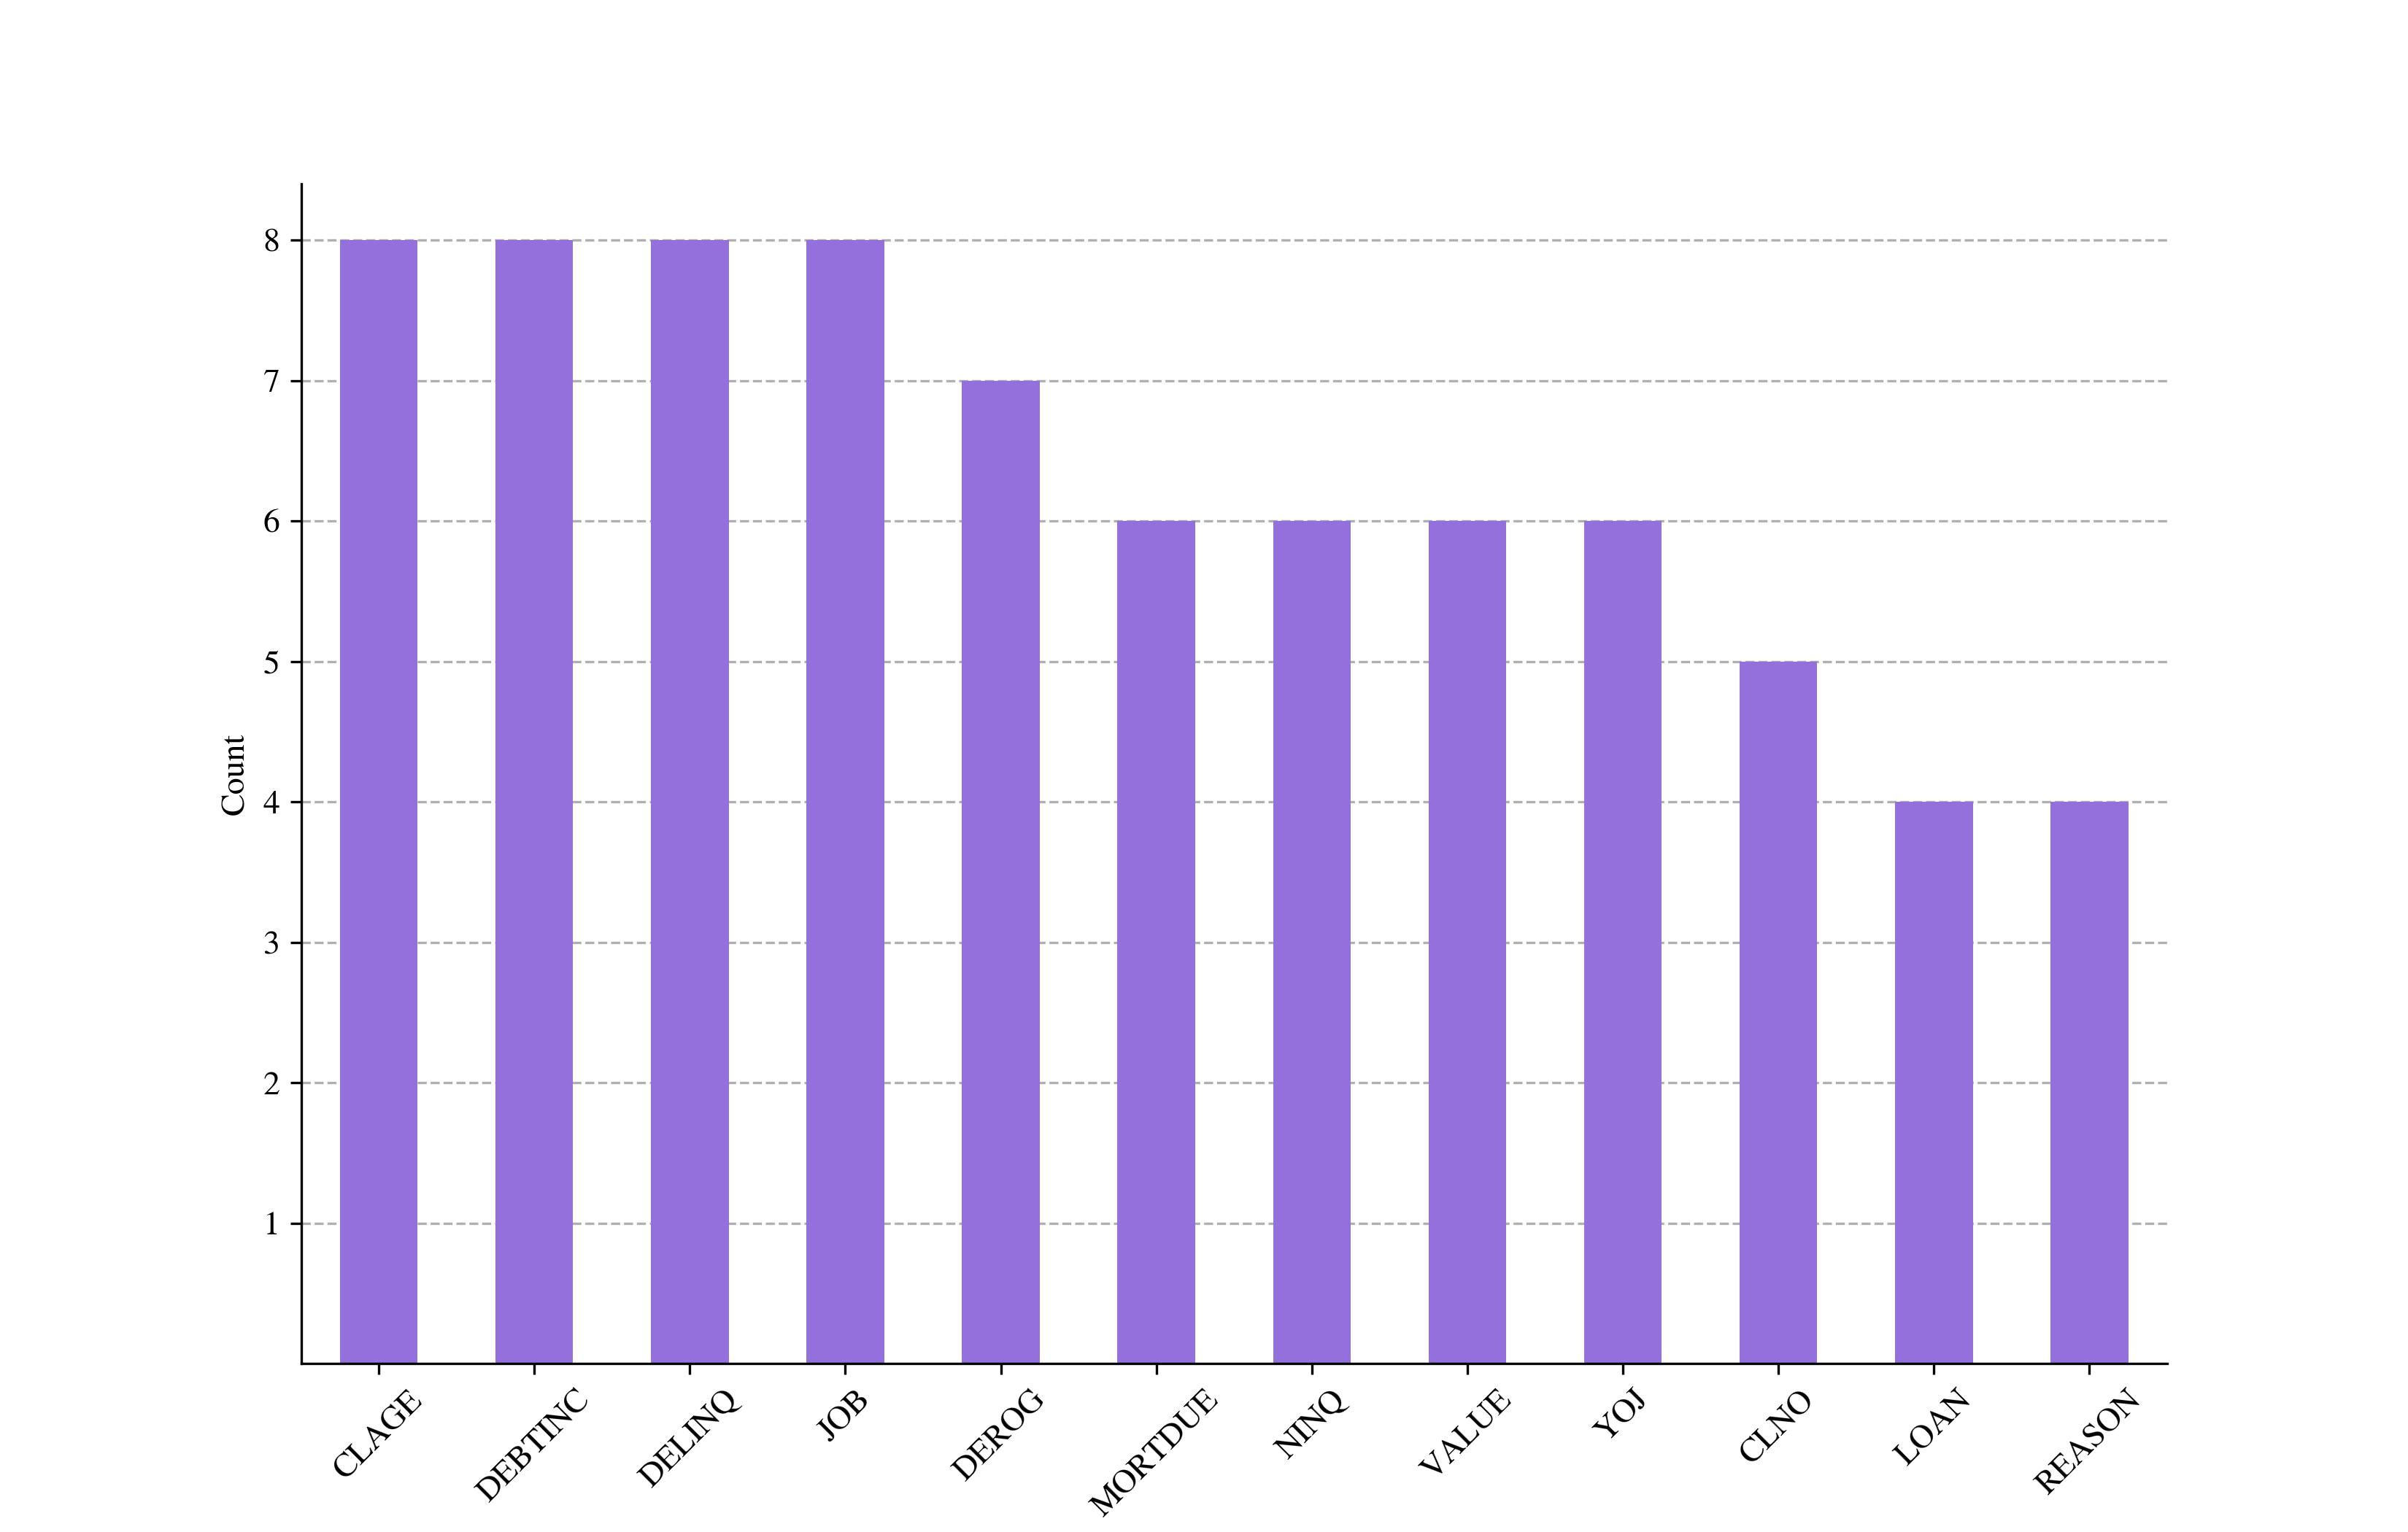
\includegraphics[width=140mm]{Figures/Recurrence_Selected_Features.jpg}
\centering{\begin{source}Author's results in Python\end{source}}\vspace{-1em}
\end{figure}


According to \autoref{fig:fsdistmod}, models such as KNN, Random Forest, Gradient Boosting and SVM chose almost all the features as onlt one feature feature was eliminated. On the other hand, Gaussian Naive Bayes chose only 6. It seems to be that most of the features are important as each model has selected a higher amount of features.
It is evident the more complex black--box models require more features in contrast to transparent models such as Logistic Regression or Gaussian Naive Bayes.
\begin{figure}[H]
    \centering
    \caption{Distribution of Selected Features per Model}\vspace{0.5em}
    \label{fig:fsdistmod}\
    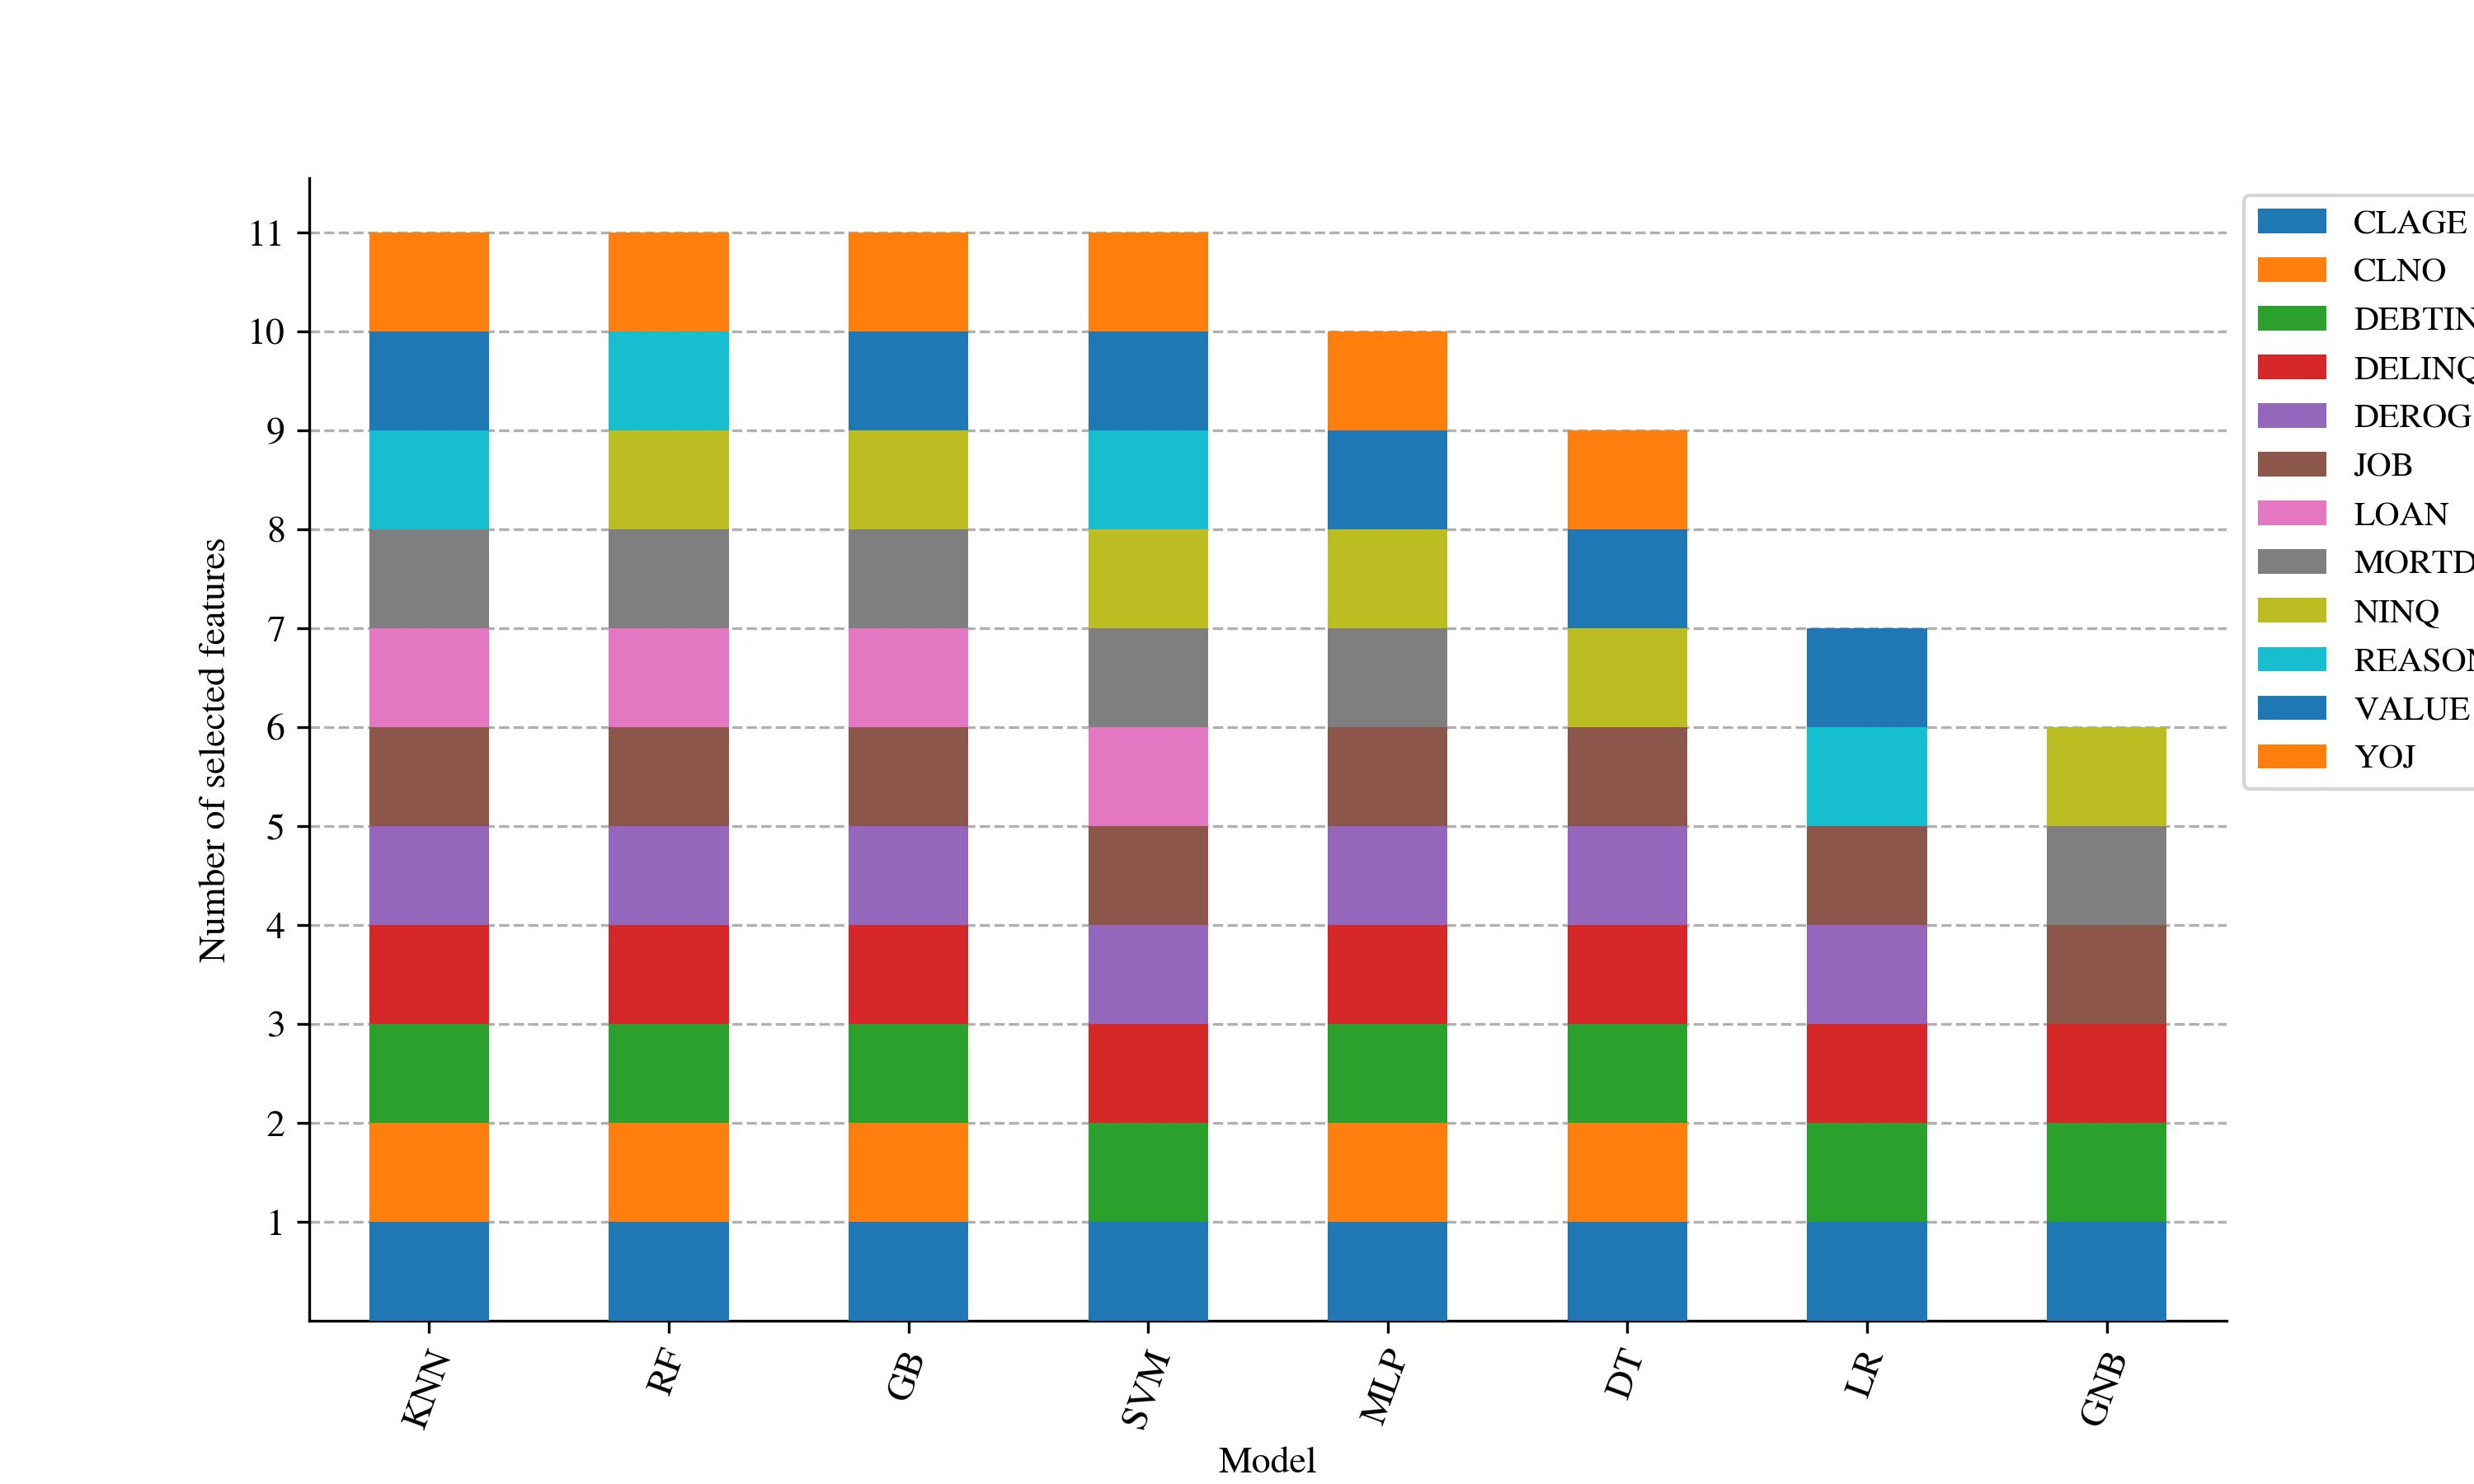
\includegraphics[width=140mm]{Figures/Selected_Features_Distribution.jpg}
    \centering{\begin{source}Author's results in Python\end{source}}\vspace{-1em}
\end{figure}

\subsection{Model Selection}

In combination with the pre--selected subsets of features, the next step regards the selection of the final model which will be further used within an evaluation and the deployment. The algorithm process is described in Algorithm  \autoref{alg:model_selection} below:
\begin{algorithm}[H]
\caption{Model Selection Algorithm}
\label{alg:model_selection}
\begin{algorithmic}[1]
\For{$model \in \textit{models}$}
    \For{$features \in \textit{features\_subsets}$}
        \State $\textit{optimized\_model} \gets \textsc{BayesianOptimization}(model, features)$
        \For{$\textit{metric} \in \textit{evaluation\_metrics}$}
            \State $\textit{performance} \gets \textsc{Evaluation}(\textit{optimized\_model}, \textit{metric})$
        \EndFor
    \EndFor
\EndFor
\end{algorithmic}
\end{algorithm}


\vspace{-1em}
Therefore, each input model is tuned on each subset of features selected within feature selection on the training set and subsequently, the optimized model is evaluated on the validation set. Thus, when having $n$ input models and $m$ subsets of selected features, we get $n \times m$ tuned models.
$m \leq n$ because we exclude duplicated subset of selected features which can occur when more than one model choose the same subset(s) of features.
Since there are 8 input models and 8 unique subsets of selected features, the total number of tuned models is 64.

\subsubsection{Metrics Space}

When evaluating classification models using class-based metrics such as F1 score, Precision, Recall, Accuracy, Matthews Correlation Coefficient, a default classification threshold of 0.5 is often used. This threshold separates predicted classes based on whether the predicted probability score is higher or lower than 0.5.
However, in real-world use cases, the 0.5 classification threshold may not be appropriate and according to \citep{esposito2021ghost}, such threshold is not appropriate when having imbalanced ata. Therefore, it is recommended to calculate an optimal threshold rather than relying on the default one.
For such case, the Youden index is employed which is derived from ROC curve and enables the selection of an optimal classification threshold value. 
The Younden index searches for the threshold that maximizes the sum of True Positive Rate and True Negative Rate, decreased by 1 \citep{fluss2005estimation}, thus:
\begin{equation}\label{eq}
J = TPR + TNR - 1
\end{equation}
Mathematically, the optimal threshold using Youden index is derived as follows:
\begin{equation}\label{eq}
T_{opt} = \text{argmax}_{t \in [0, 1]}\left(J\right)
\end{equation}
In Python, the \lstinline{roc_curve} function from \lstinline{Scikit-learn} returns False Positive Rate instead of the True Negative Rate. Nevertheless, we can derive the True Negative Rate from False Positive Rate as follows:
\begin{equation}\label{eq}
TNR =  1-FPR
\end{equation}
Therefore:
\begin{equation}\label{eq}
T_{opt} = \text{argmax}_{t \in [0, 1]}\left(TPR +  \left(1-FPR\right) - 1\right)
\end{equation}
Note, that the optimal threshold is calculated based on the training set and henceforth is applied within the evaluation on validation set.

In order to ensure a more comprehensive and unbiased evaluation of a model's performance, it is recommended to consider multiple metrics rather than relying on a single metric alone. This approach provides a more generalized overview of the model's performance across different aspects and helps to prevent any bias towards a single metric.
To accomplish this, models can be ranked based on their performance on each individual metric, where a higher score or a lower loss indicates a better model, resulting in a higher rank for that metric. Subsequently, for each metric, the ranking of the models is determined, and the final ranking is calculated as a weighted average of these individual rankings.
The weights have been set expertly and are summarized in \autoref{tab:weightsrank}.

Specifically, the highest weight (1.5) is assigned to the F1 score, which provides a balanced measure of a model's performance with respect to both False Positives and False Negatives.
This metric is commonly used in classification tasks, particularly in imbalanced data sets, such as the validation set in our case, which has not been oversampled.
In addition to the F1 score, higher weight is assigned to the Recall score as well (1.2), which is a metric that penalizes False Negatives.
False Negatives occur when the model predicts a negative result (i.e., no default) for an instance that is actually positive (i.e., default).
In the context of loan applications, one may prefer to reject a loan applicant who would not have defaulted (False Positive) rather than approving the application of a client who would have defaulted (False Negative). Therefore, it is appropriate to give higher weight to Recall in order to reduce the likelihood of False Negatives.
Henceforth, the weights are assigned to different metrics based on their relevance to the models' ranking, with the highest weight given to F1 score and additional weight given to Recall to ensure that False Negatives are minimized.

\begin{table}[H]
\small
\setlength{\tabcolsep}{8pt}
\renewcommand{\arraystretch}{1.3}
\centering
    \caption[Model Ranking Weights]{Model Ranking Weights}\label{tab:weightsrank}
    \begin{tabular}{>{\raggedleft\arraybackslash}p{0.4\linewidth} l}
\toprule
\textbf{Metric} & \textbf{Weight}\\
\midrule
\hline
F1 score & 1.5 \\
Recall & 1.2 \\
Precision & 1 \\
Accuracy & 1 \\
AUC & 1 \\
Somers' D & 1 \\ 
Kolmogorov Smirnov & 1 \\
Matthews Correlation Coefficient  & 1 \\
Brier Score Loss  & 1 \\
\hline
\bottomrule
\end{tabular}
\vspace{0.7em}

\centering{\begin{source}Author's results in Python\end{source}}\vspace{-1em}
\end{table}

Particularly, for each model a rank score is calculated in order to determine the final rank. The lower rank score indicates better model performance. For particular model $M$, the rank score as weighted sum of the individual ranks as follows:
\begin{equation}\label{eq:rankscorem}
    RankScore_{M} = \frac{\sum_{i=1}^{k} {r_i \times w_i}}{\sum_{i=1}^{k} {w_i}} 
\end{equation}
where $k$ is the number of metrics used to evaluated the model $M$, $r_i$ is the rank order of $i$--th metric for given model $M$ and $w_i$ is the weight assigned to the $i$--th metric.
Such metric lies in interval $<1, k>$, where 1 would indicate a perfect model performance across the all metrics.

\subsubsection{Model Selection Results}



The custom function \lstinline{model_selection()} iteratively prints the process of the model tuning and evaluation on each subset of features, in order to keep the track of such process as it is depicted in \autoref{fig:modselprint}.
Particularly, it prints which model on which features is being tuned and evaluated, exeuction time, optimal threshold, F1 score on the validation set and the best hyperparameters.

\begin{figure}[H]
\centering\caption{Model Selection Print Statement}
\label{fig:modselprint}

{\fontsize{8.8}{11}\selectfont 
\begin{verbatim}
-------------------------------------------------------------------------------------
--------------------------------------- 56/64 ---------------------------------------
-------------------------------------------------------------------------------------
---------------------------- BAYESIAN OPTIMIZATION OF SVM ---------------------------
--------------------------- WITH FEATURES SELECTED BY MLP ---------------------------
-------------------------------------------------------------------------------------
------------------------------------------------------------------------------------- 

1/2 ... Starting Bayesian Optimization on the subset of features (10 features):
        MORTDUE, VALUE, JOB, YOJ, DEROG, DELINQ, CLAGE, NINQ, CLNO, DEBTINC
2/2... Bayesian Optimization finished 

Execution time: 22.0695 minutes 

F1 Score on Validation set: 0.7102272727272726 

Optimal classification threshold: 0.6477 

Tuned hyperparameters of SVM: 

    C: 4.999999999999999
    break_ties: False
    cache_size: 200
    class_weight: balanced
    coef0: 0.0
    decision_function_shape: ovr
    degree: 1
    gamma: scale
    kernel: rbf
    max_iter: -1
    probability: True
    random_state: 42
    shrinking: False
    tol: 1.102507160381566e-09
    verbose: False

-------------------------------------------------------------------------------------
------------------------------------------------------------------------------------- 
\end{verbatim}
}
\centering{\begin{source}Author's results in Python\end{source}}\vspace{0em}
\end{figure}



The final output of the function \lstinline{model_selection()} is table which summarizes the model's computed metrics as depicted in \autoref{tab:modelsectab}. As can be seen, the best models in terms of ranking are the Gradient Boosting models which in general have the highest score metrics and the lowest loss metrics. On the other hand, the worst-performing models are Gaussian Naive Bayes models.


\clearpage
\newpage

\KOMAoptions{paper=landscape,DIV=last}
\newgeometry{hmargin=2.5cm,bottom=25mm,height=150mm,includehead}
\fancyheadoffset{0pt}



\begin{table}[H]
\small
\setlength{\tabcolsep}{8pt}
\renewcommand{\arraystretch}{1.3}
\caption[Model Selection Results]{Model Selection Results}\label{tab:modelsectab}
\centering
\scalebox{0.8}{

\begin{tabular}{|p{1.3cm}|p{1.3cm}|>{\raggedleft}p{1.5cm}|>{\raggedleft}p{1.3cm}|c|c|c|c|c|c|c|c|c|c|c|c||c|c|}
    \toprule
    \textbf{Tuned model} & \textbf{FS model} & \textbf{\# \newline Features} & \textbf{Exec. \newline Time} & \textbf{Thresh.} & \textbf{F1} & \textbf{Prec.} & \textbf{Rec.} & \textbf{Acc.} & \textbf{AUC} & \textbf{SD} & \textbf{KS} & \textbf{MCC} & \textbf{BS} & \textbf{Log Loss} & \textbf{Score} & \textbf{Rank} \\
    \midrule
    \hline
GB & MLP & 10 & 738.19 & 0.4955 & 0.7809 & 0.7853 & 0.7765 & 0.9128 & 0.9515 & 0.9030 & 0.7751 & 0.7265 & 0.0666 & 0.2487 & 3.48 & 1 \\ 
GB & KNN & 11 & 767.90 & 0.5072 & 0.7978 & 0.7912 & 0.8045 & 0.9184 & 0.9587 & 0.9175 & 0.7989 & 0.7467 & 0.0687 & 0.4135 & 3.82 & 2 \\ 
GB & SVM & 11 & 904.84 & 0.5053 & 0.7896 & 0.8155 & 0.7654 & 0.9184 & 0.9555 & 0.9109 & 0.7961 & 0.7397 & 0.0718 & 0.3486 & 4.17 & 3 \\ 
GB & GB & 11 & 686.26 & 0.4132 & 0.7799 & 0.7778 & 0.7821 & 0.9117 & 0.9543 & 0.9086 & 0.7989 & 0.7247 & 0.0703 & 0.3372 & 4.29 & 4 \\ 
GB & RF & 11 & 802.55 & 0.4973 & 0.7775 & 0.7841 & 0.7710 & 0.9117 & 0.9541 & 0.9081 & 0.7961 & 0.7225 & 0.0669 & 0.2803 & 4.37 & 5 \\ 
RF & KNN & 11 & 356.24 & 0.4725 & 0.7486 & 0.7326 & 0.7654 & 0.8972 & 0.9226 & 0.8452 & 0.7109 & 0.6843 & 0.0923 & 0.3232 & 8.66 & 6 \\ 
GB & DT & 9 & 719.92 & 0.4729 & 0.7675 & 0.7697 & 0.7654 & 0.9073 & 0.9407 & 0.8814 & 0.7556 & 0.7096  & 0.0808 & 0.4693 & 8.87 & 7 \\ 
RF & GB & 11 & 310.63 & 0.4517 & 0.7385 & 0.7135 & 0.7654 & 0.8916 & 0.9200 & 0.8400 & 0.7123 & 0.6709 & 0.0886 & 0.3135 & 9.47 & 8 \\ 
RF & MLP & 10 & 397.42 & 0.4761 & 0.7357 & 0.7181 & 0.7542 & 0.8916 & 0.9179 & 0.8358 & 0.7081 & 0.6679 & 0.0879 & 0.3084 & 10.39 & 9 \\ 
GB & LR & 7 & 1008.69 & 0.4362 & 0.7388 & 0.7000 & 0.7821 & 0.8894 & 0.9219 & 0.8438 & 0.7081 & 0.6706 & 0.0886 & 0.3925 & 10.79 & 10 \\ 
\ldots & \ldots & \ldots & \ldots & \ldots & \ldots & \ldots & \ldots & \ldots & \ldots & \ldots & \ldots & \ldots & \ldots & \ldots & \ldots & \ldots \\
DT & MLP & 10 & 54.19 & 0.5000 & 0.6427 & 0.6374 & 0.6480 & 0.8559 & 0.8133 & 0.6266 & 0.5810 & 0.5524 & 0.1254 & 2.0008 & 50.38 & 55 \\ 
GNB & GB & 11 & 23.04 & 0.1829 & 0.5970 & 0.4893 & 0.7654 & 0.7933 & 0.8531 & 0.7063 & 0.5810 & 0.4880 & 0.1310 & 0.6461 & 50.50 & 56 \\ 
GNB & KNN & 11 & 22.98 & 0.3588 & 0.6093 & 0.5219 & 0.7318 & 0.8123 & 0.8479 & 0.6957 & 0.5698 & 0.5024 & 0.1367 & 0.6686 & 50.81 & 57 \\ 
GNB & DT & 9 & 23.11 & 0.2241 & 0.6063 & 0.5095 & 0.7486 & 0.8056 & 0.8467 & 0.6935 & 0.5768 & 0.4991 & 0.1316 & 0.6370 & 50.85 & 58 \\ 
GNB & MLP & 10 & 23.11 & 0.2194 & 0.6013 & 0.5000 & 0.7542 & 0.8000 & 0.8493 & 0.6986 & 0.5768 & 0.4930 & 0.1319 & 0.6360 & 50.99 & 59 \\ 
DT & GNB & 6 & 53.14 & 0.5000 & 0.6354 & 0.6284 & 0.6425 & 0.8525 & 0.8187 & 0.6375 & 0.5838 & 0.5430 & 0.1251 & 2.1679 & 51.74 & 60 \\ 
GNB & GNB & 6 & 23.05 & 0.4787 & 0.5950 & 0.5039 & 0.7263 & 0.8022 & 0.8356 & 0.6711 & 0.5559 & 0.4835 & 0.1470 & 0.5280 & 54.53 & 61 \\ 
LR & GNB & 6 & 95.14 & 0.4561 & 0.5948 & 0.5121 & 0.7095 & 0.8067 & 0.8379 & 0.6758 & 0.5531 & 0.4831 & 0.1319 & 0.4180 & 54.97 & 62 \\ 
GNB & SVM & 11 & 22.91 & 0.1991 & 0.5885 & 0.4872 & 0.7430 & 0.7922 & 0.8425 & 0.6850 & 0.5712 & 0.4756 & 0.1345 & 0.6721 & 55.15 & 63 \\ 
GNB & RF & 11 & 23.25 & 0.3413 & 0.5864 & 0.4943 & 0.7207 & 0.7966 & 0.8288 & 0.6577 & 0.5545 & 0.4720 & 0.1486 & 0.7040 & 57.85 & 64 \\ 
    \hline
    \bottomrule 
\end{tabular}}
\vspace{1em}

\centering{\begin{source}Author's results in Python\end{source}}\vspace{-1em}
\end{table}

\clearpage
\newpage
\KOMAoptions{paper=portrait,DIV=last}
\restoregeometry
\fancyheadoffset{0pt}

In order to gain a more detailed understanding of the model selection results, the distribution of computed metrics is plotted. In \autoref{fig:f1dist}, the F1 score distribution is visualized for each input model. An outlier can be observed in KNN where the F1 score is 0.				
\begin{figure}[H]
\centering
\caption{F1 Score Distribution}\vspace{0.5em}
\label{fig:f1dist}\
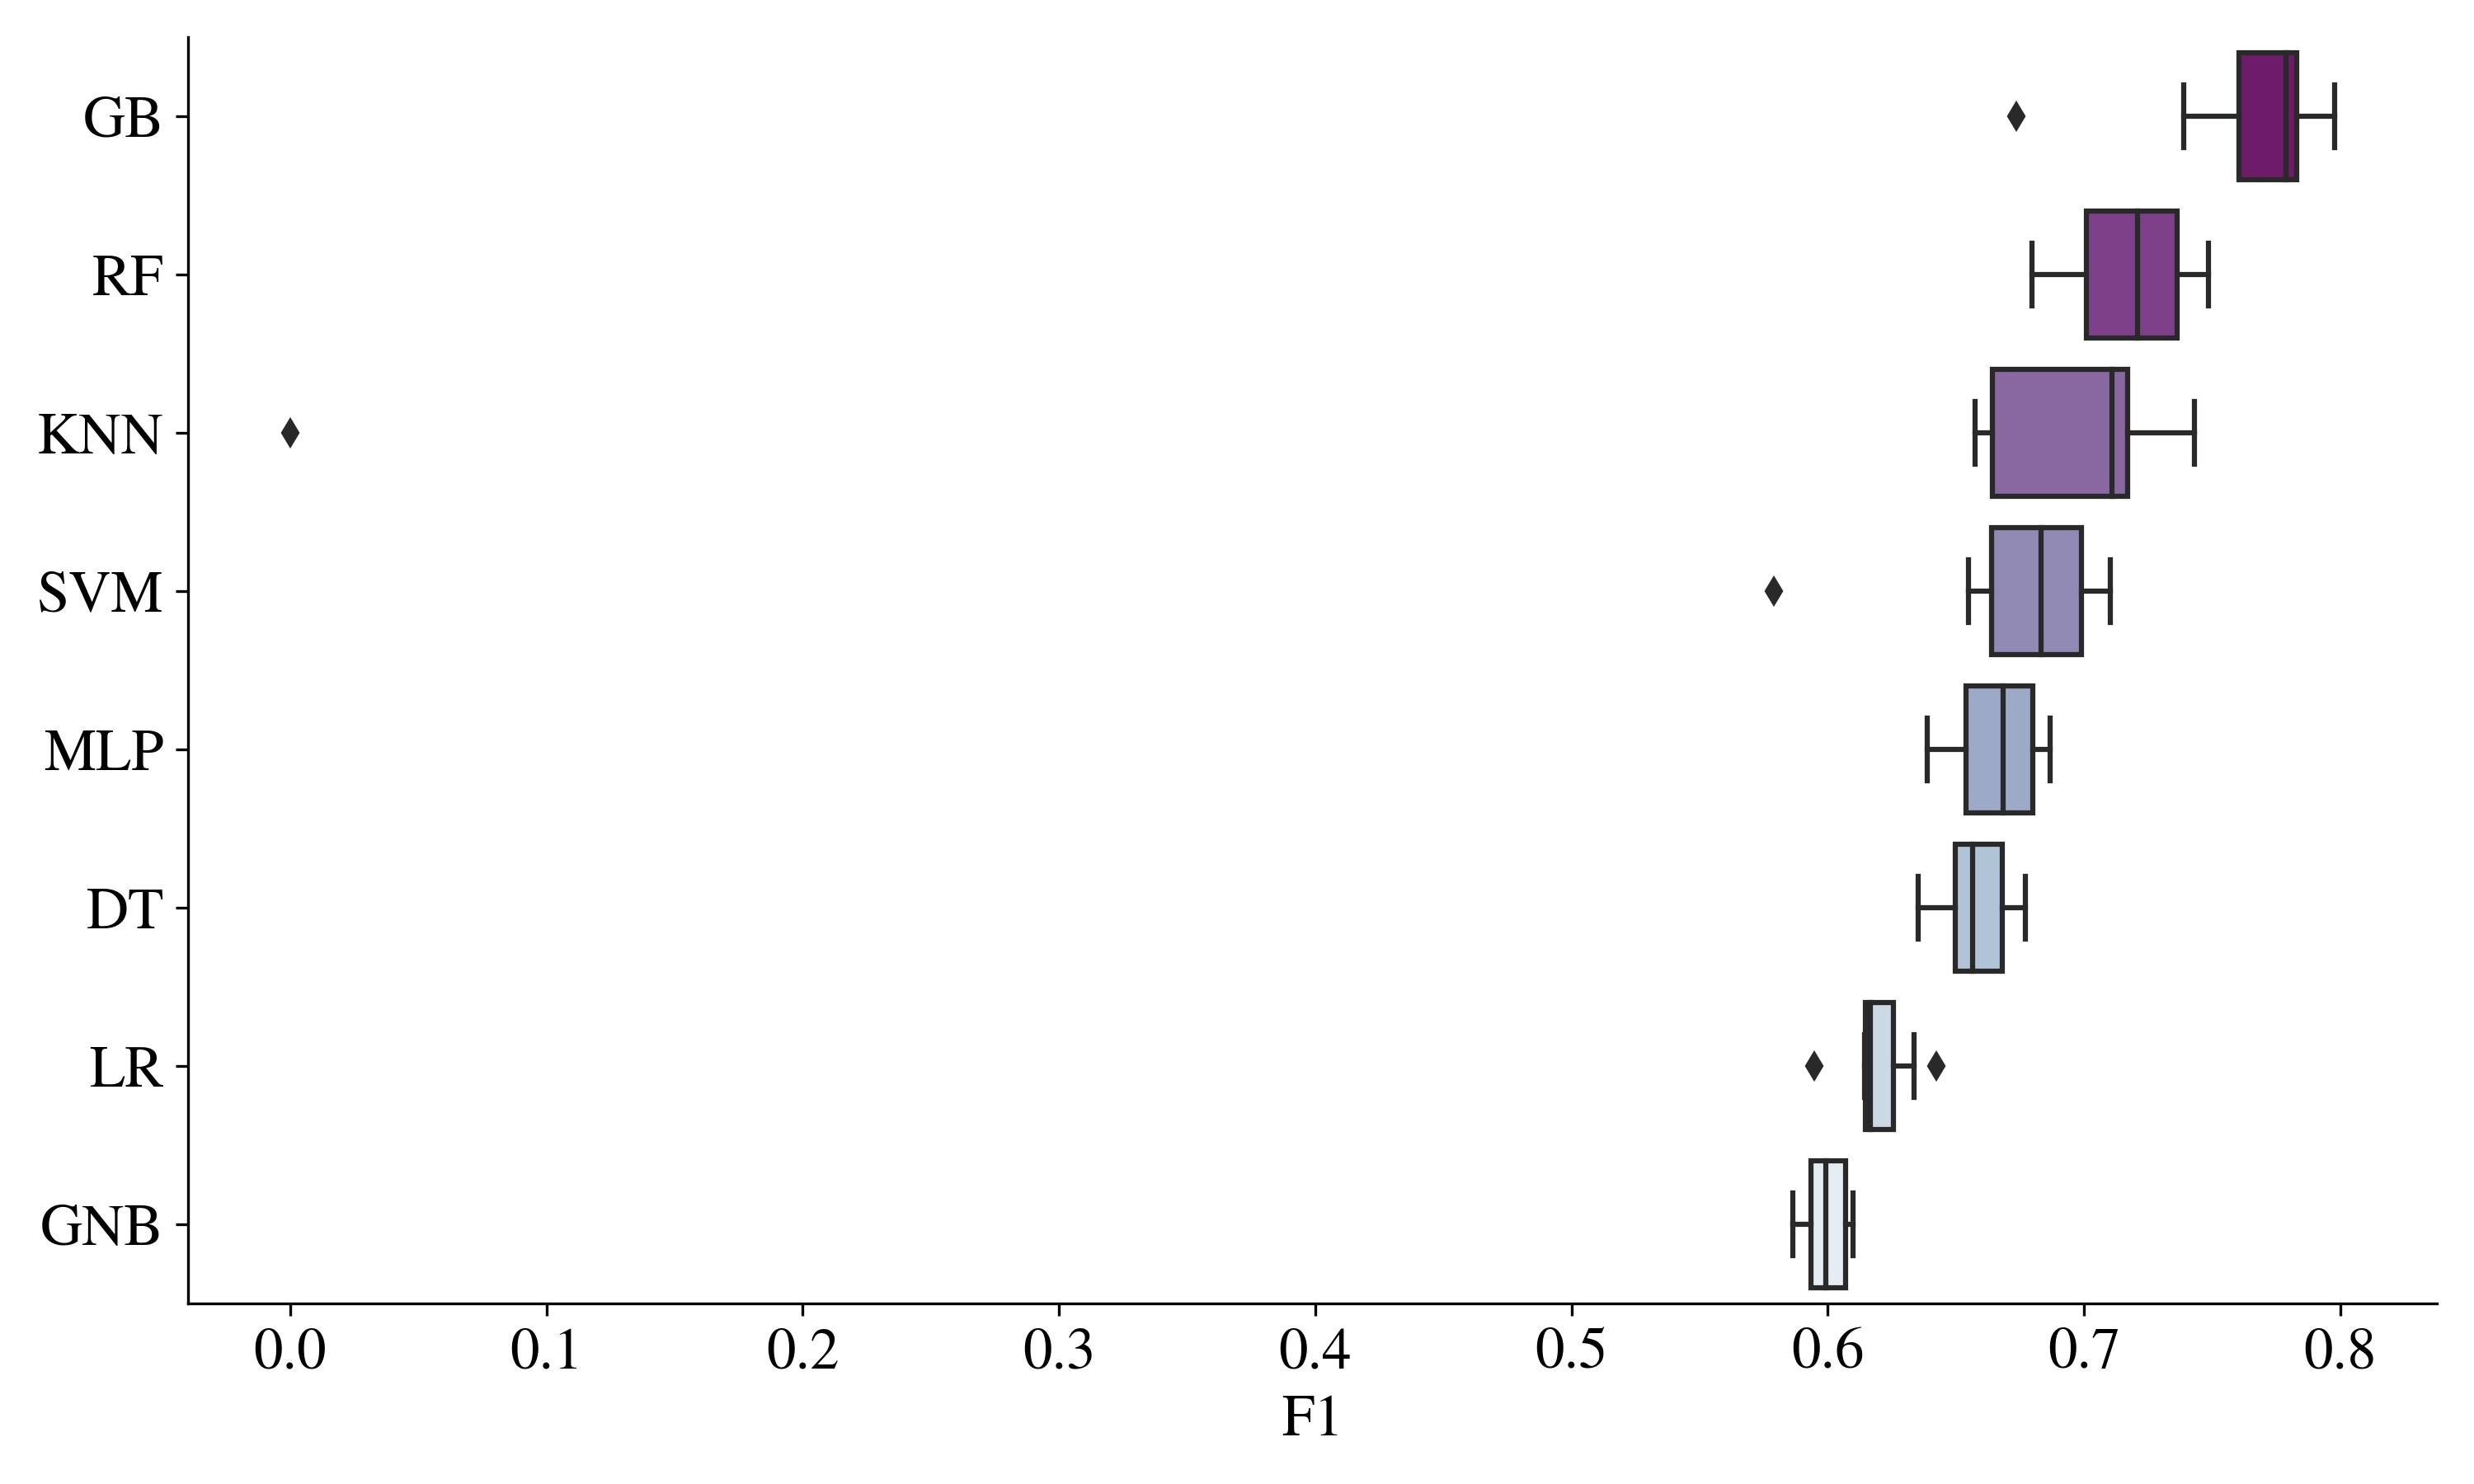
\includegraphics[width=140mm]{Figures/F1_Distribution.jpg}
\centering{\begin{source}Author's results in Python\end{source}}\vspace{-1em}
\end{figure}
Such outlier is removed in \autoref{fig:f1distclean} to gain a more general insight into the F1 score distribution.
It can be observed that Gradient Boosting models have the highest F1 scores of around 80 \%.
Another tree ensemble model, Random Forest, is performing well as the second best. However, more transparent models such as Logistic Regression and Naive Bayes are performing poorly, having F1 scores around 60 \%.
\begin{figure}[H]
\centering
\caption{F1 Score Distribution - \textit{without outlier}}\vspace{0.5em}
\label{fig:f1distclean}\
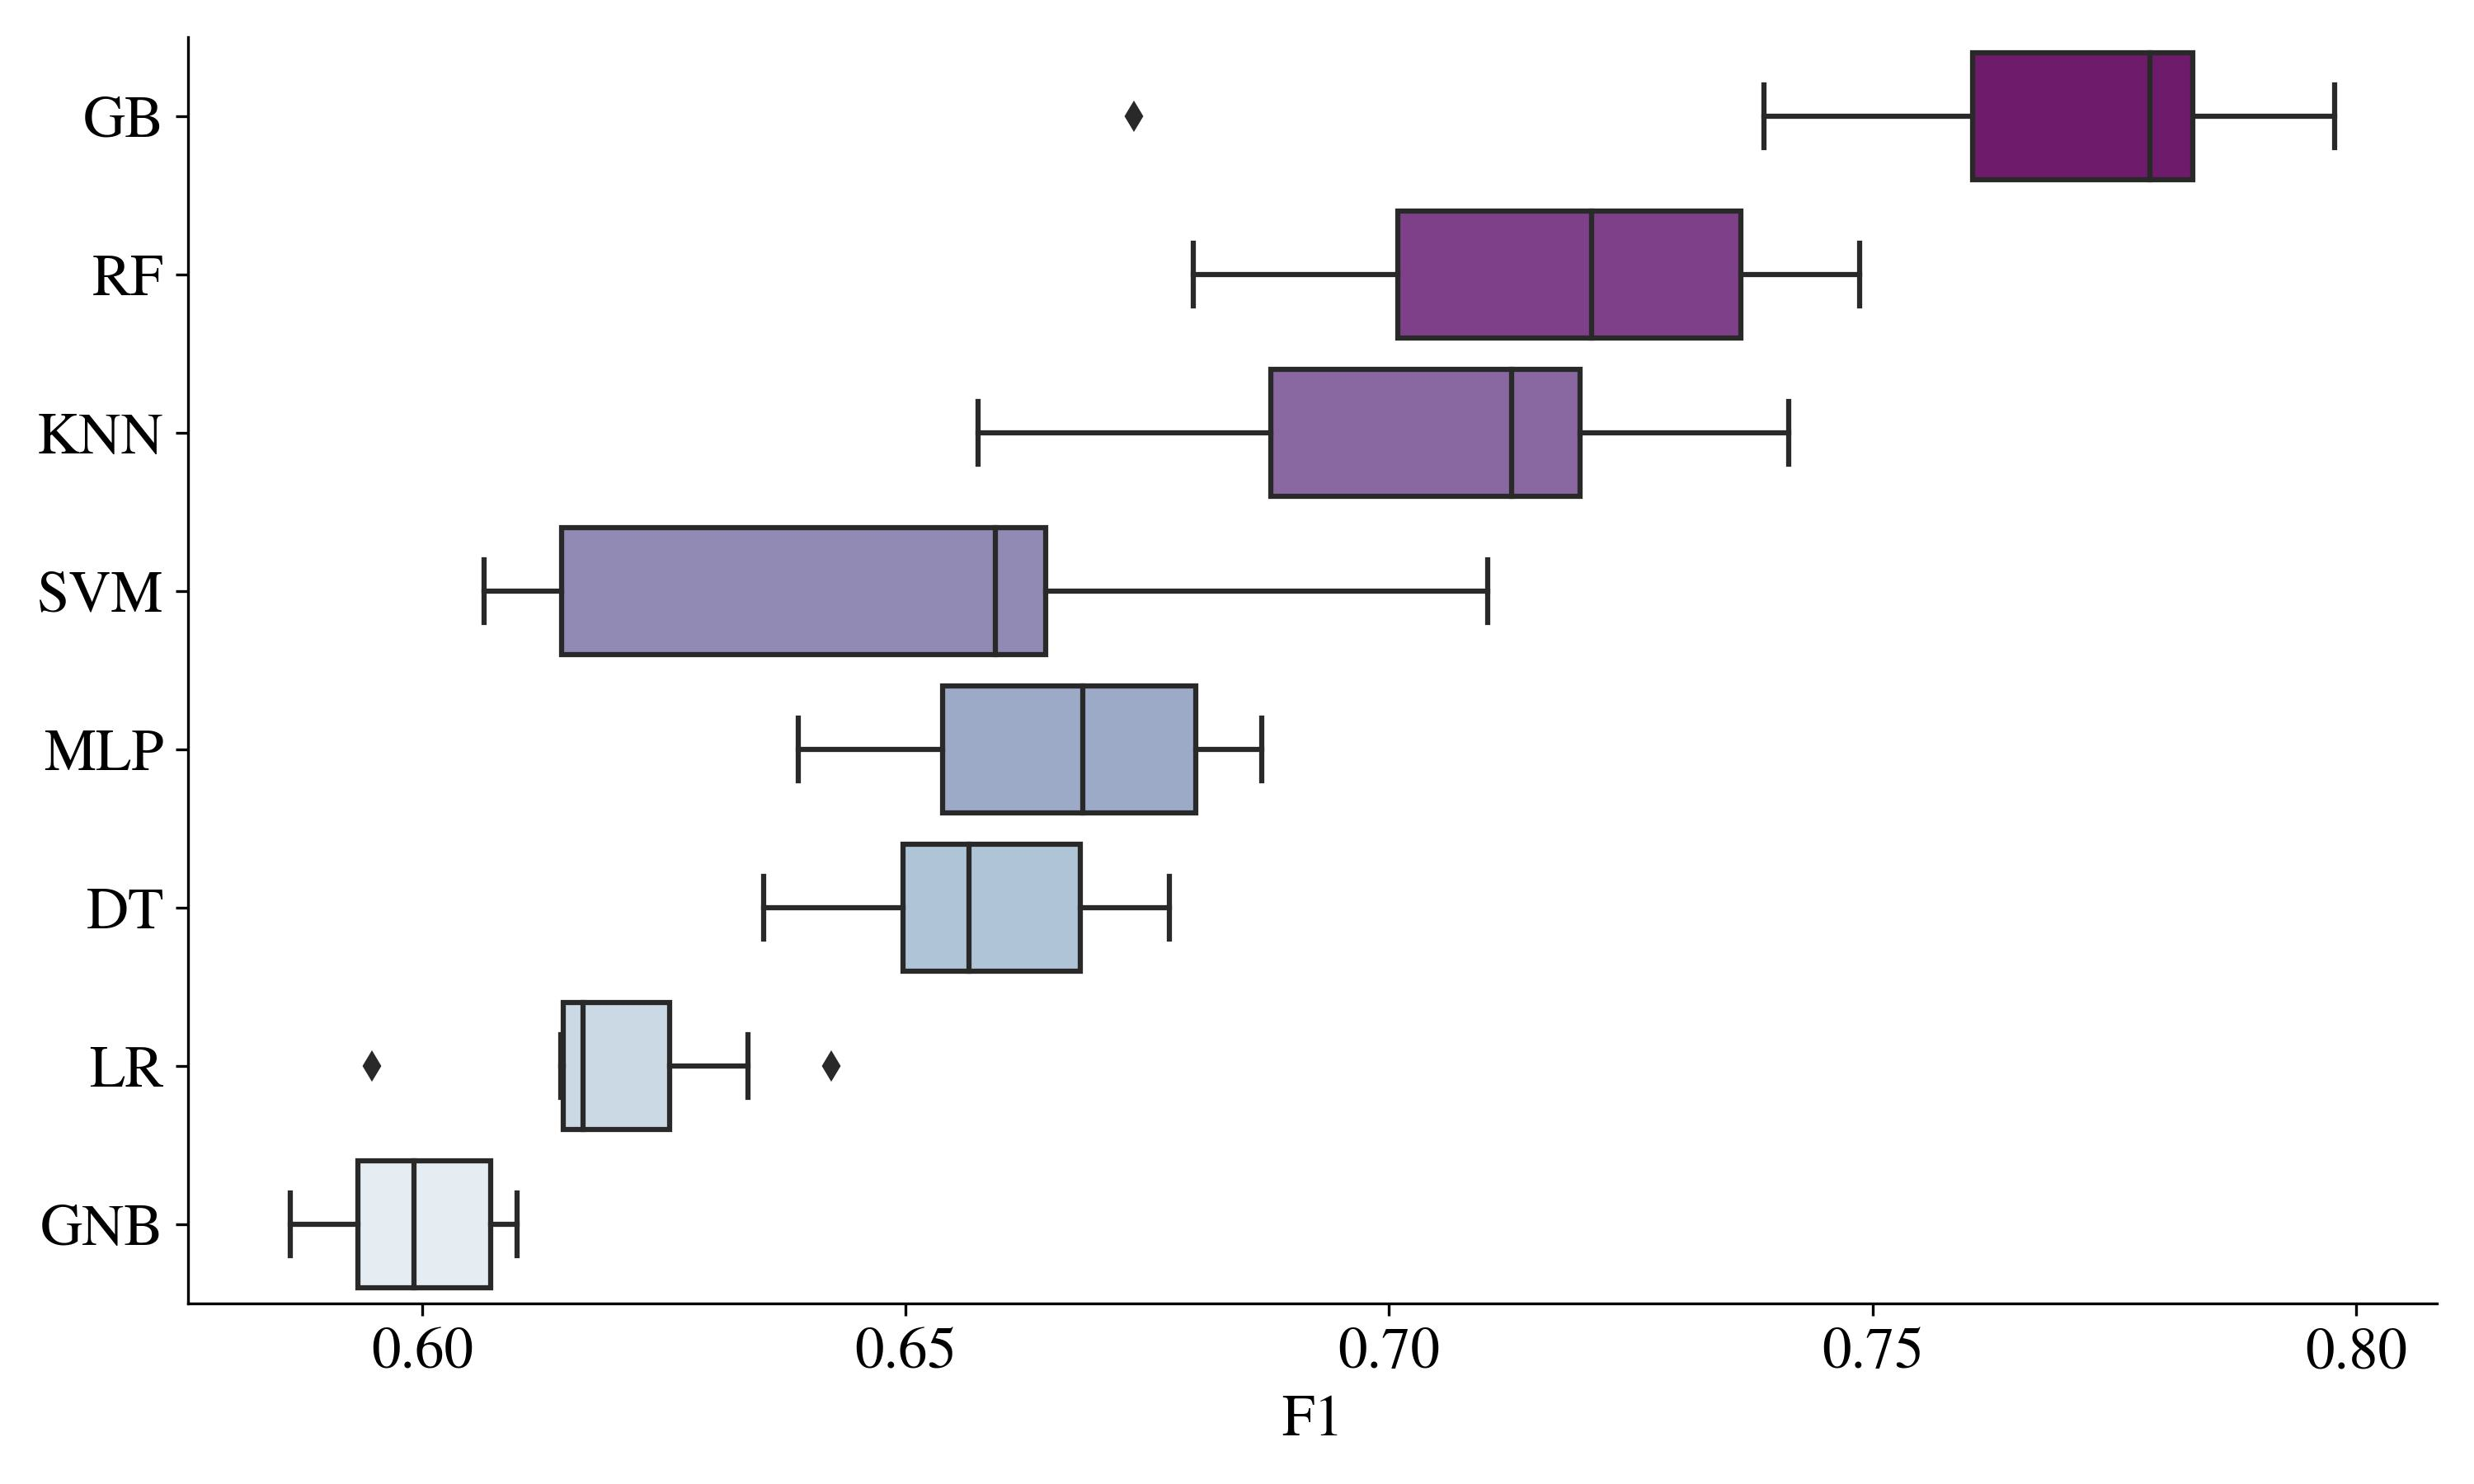
\includegraphics[width=140mm]{Figures/F1_wo_outliers_Distribution.jpg}
\centering{\begin{source}Author's results in Python\end{source}}\vspace{-1em}
\end{figure}

As depicted in \autoref{fig:f1distcleanbbwb}, it visualizes the distribution of F1 score (without the outlier) across the model type. Although, both score distributions overlap, it is evident, that black--box models outperform white--box model in terms of F1 score in overall as expected.
\begin{figure}[H]
    \centering
    \caption{F1 Score Distribution (Black--box/White--box dimension) - \textit{without outlier}}\vspace{0.5em}
    \label{fig:f1distcleanbbwb}\
    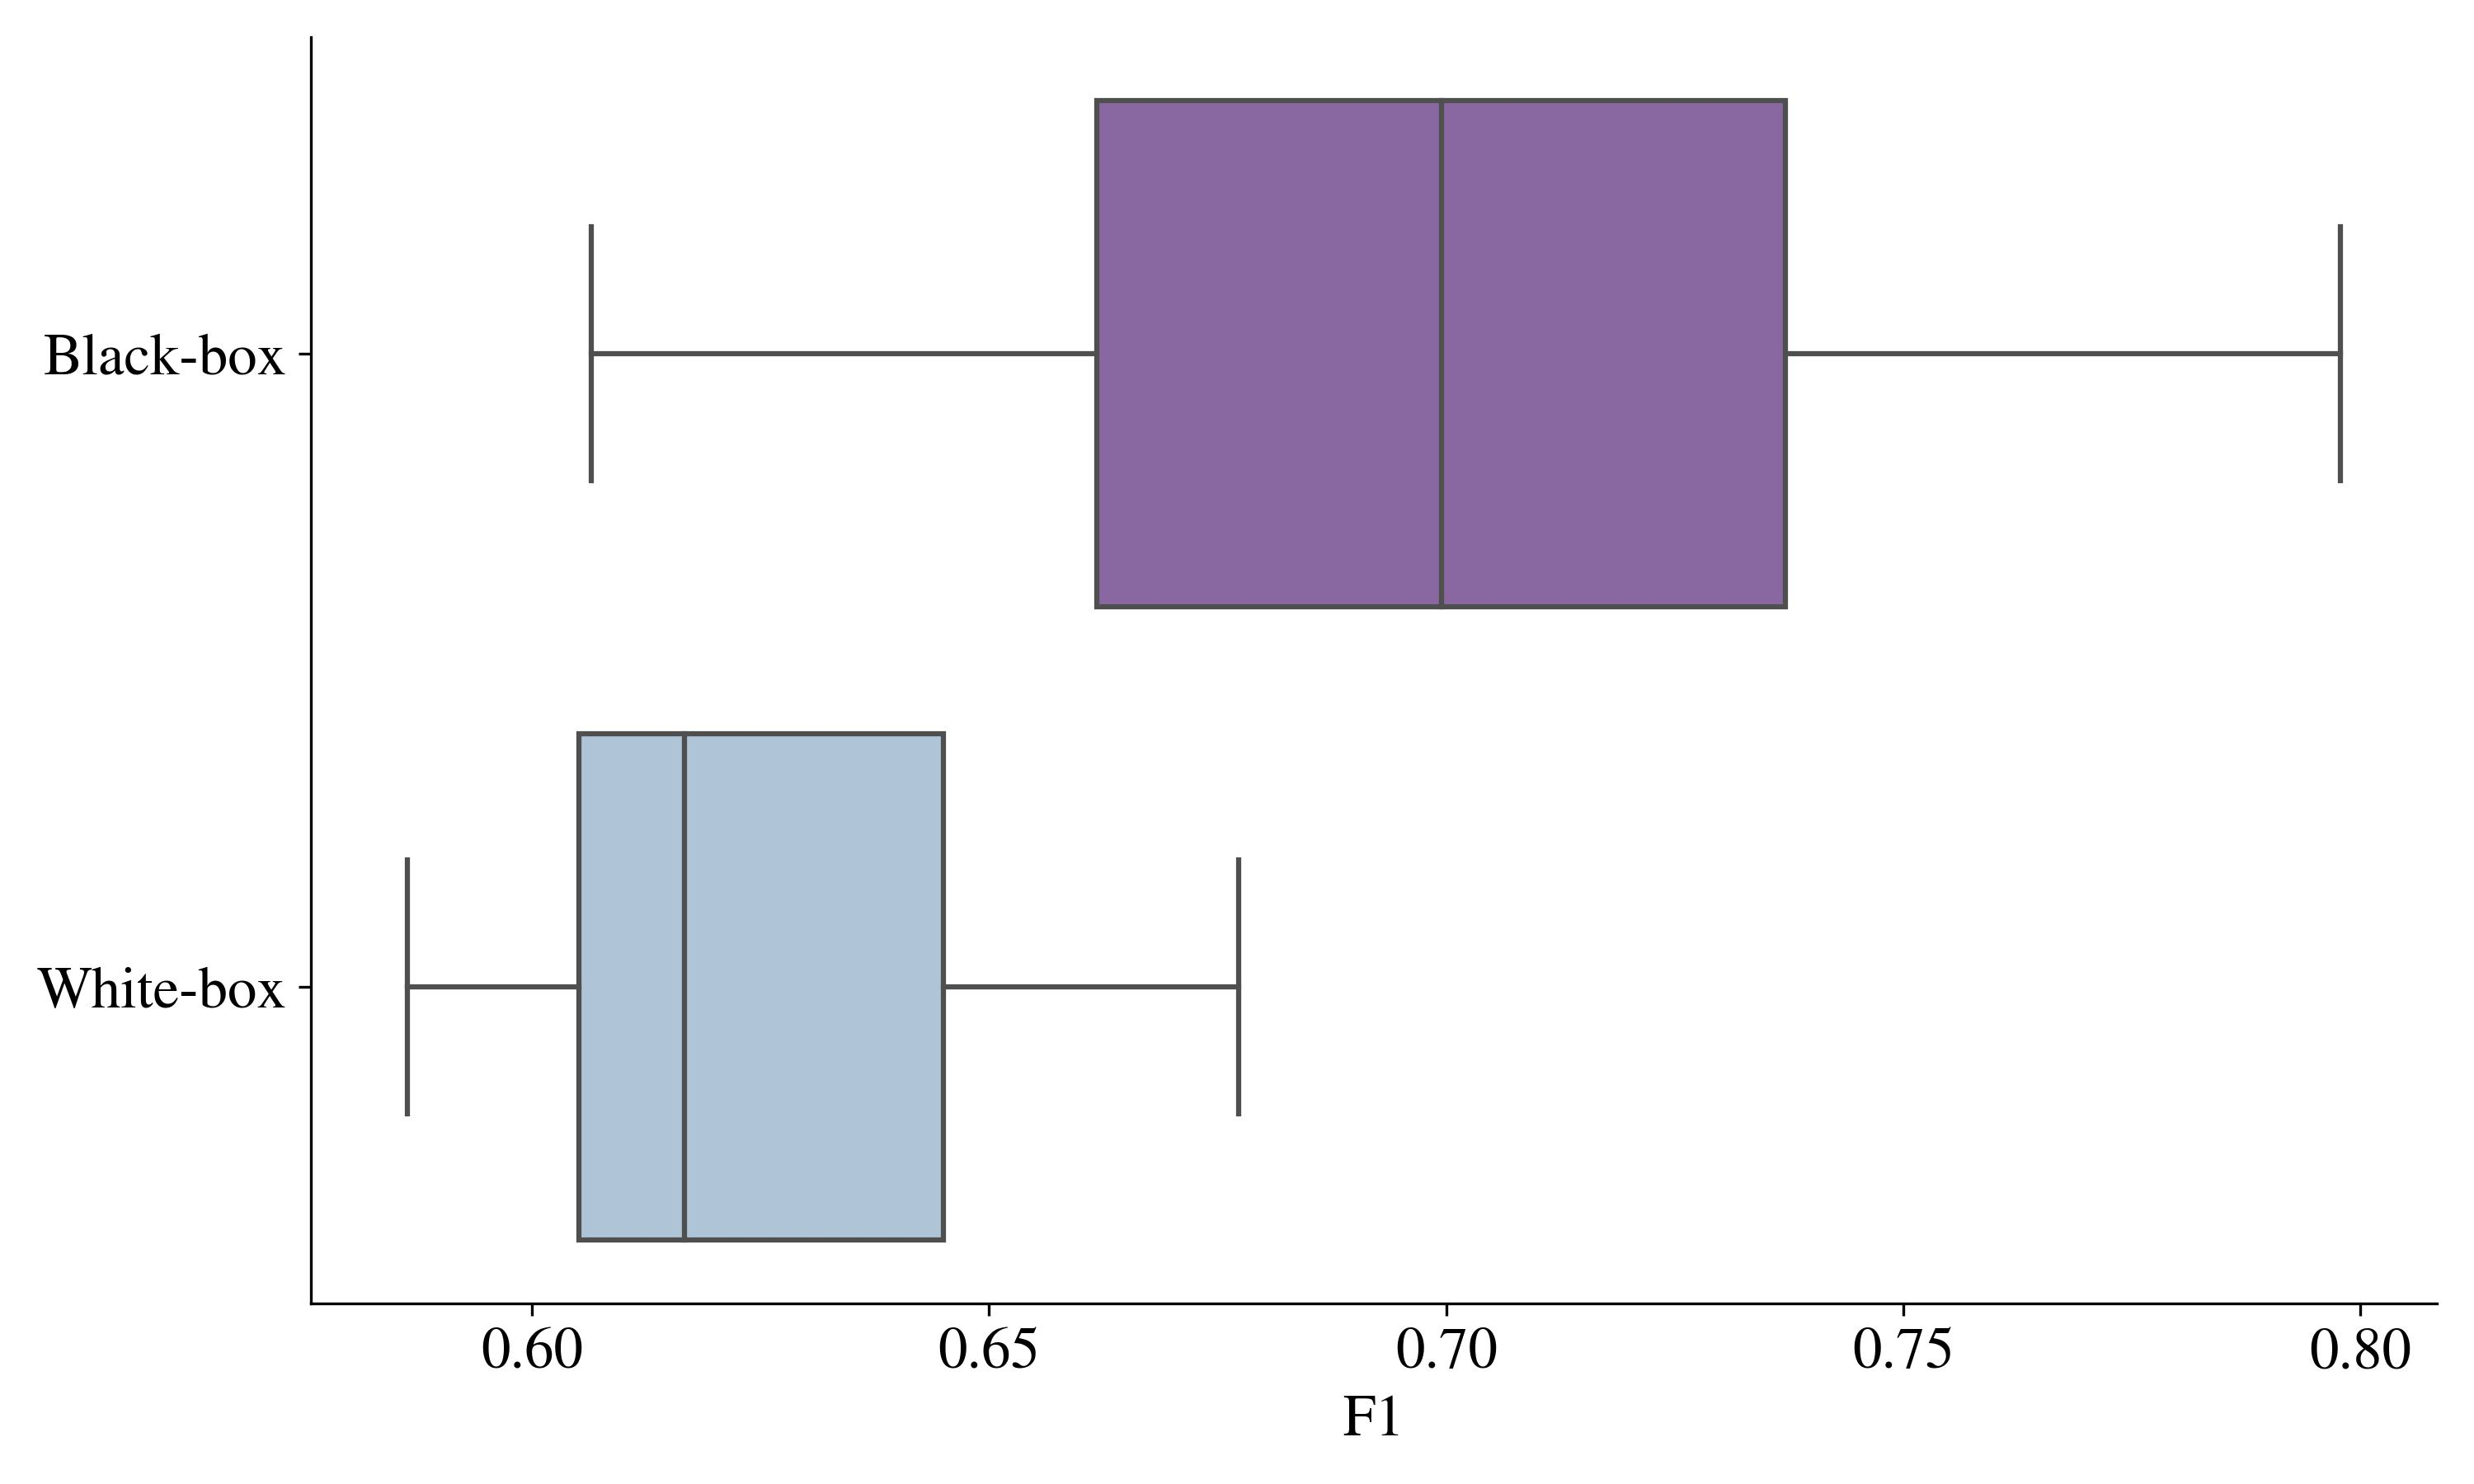
\includegraphics[width=140mm]{Figures/F1_wo_outliers_Distribution_BB_WB.jpg}
    \centering{\begin{source}Author's results in Python\end{source}}\vspace{-1em}
\end{figure}

We can also consider not only F1 score but also other metrics, which is quantified in the rank score calculated according to \autoref{eq:rankscorem}. As shown in \autoref{fig:avgrankdist}, we can observe that the order of models ranked by the rank score is identical as the order of the models ranked by F1 score in \autoref{fig:f1dist}.
Hence, across all the metrics, the Gradient Boosting perform the best in overall while Gaussian Naive Bayes does not perform well at all.
\begin{figure}[H]
    \centering
    \caption{Rank Score Distribution}\vspace{0.5em}
    \label{fig:avgrankdist}\
    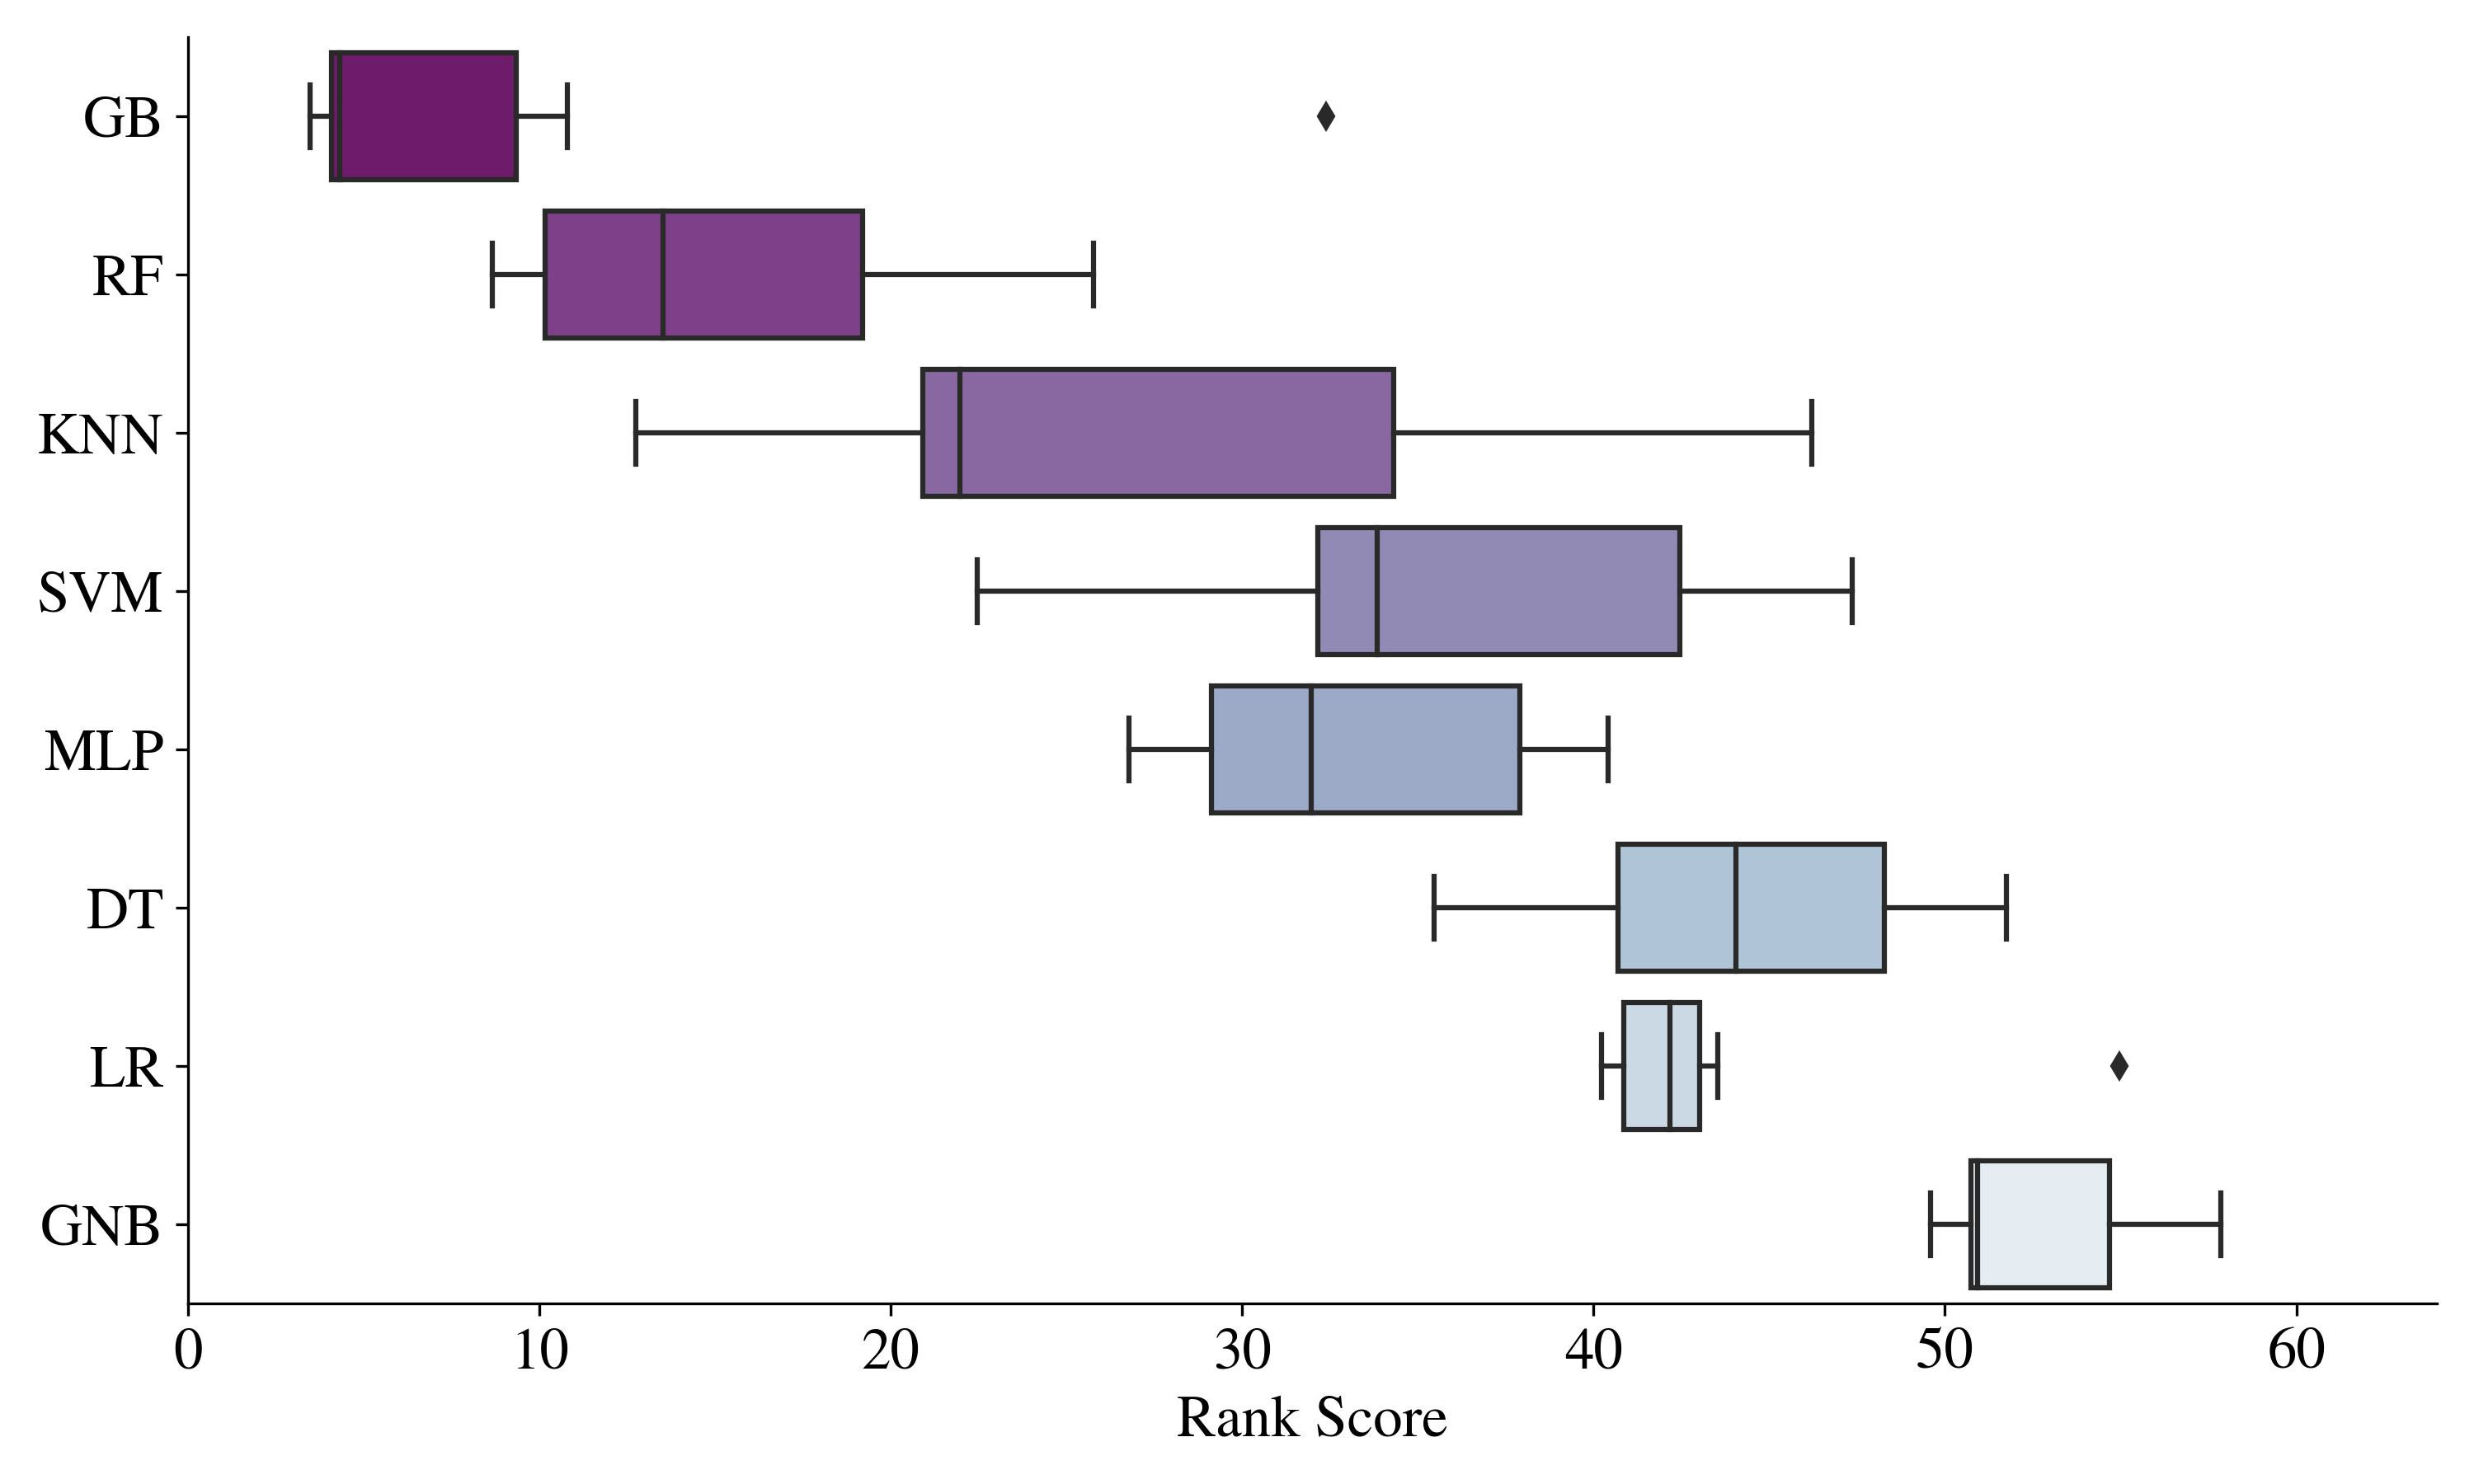
\includegraphics[width=140mm]{Figures/AVG_Rank_score_Distribution.jpg}
    \centering{\begin{source}Author's results in Python\end{source}}\vspace{-1em}
\end{figure}

As expected, also, the black--box models are ranked higher than the white--box models according to the rank score as shown in \autoref{fig:avgrankdistbbwb}. This is evident also from \autoref{tab:modelsectab} where the black--box models, namely Gradient Boosting and Random Forest, dominated amongst the first 10 ranked models.
\begin{figure}[H]
    \centering
    \caption{Rank Score Distribution (Black--box/White--box dimension)}\vspace{0.5em}
    \label{fig:avgrankdistbbwb}\
    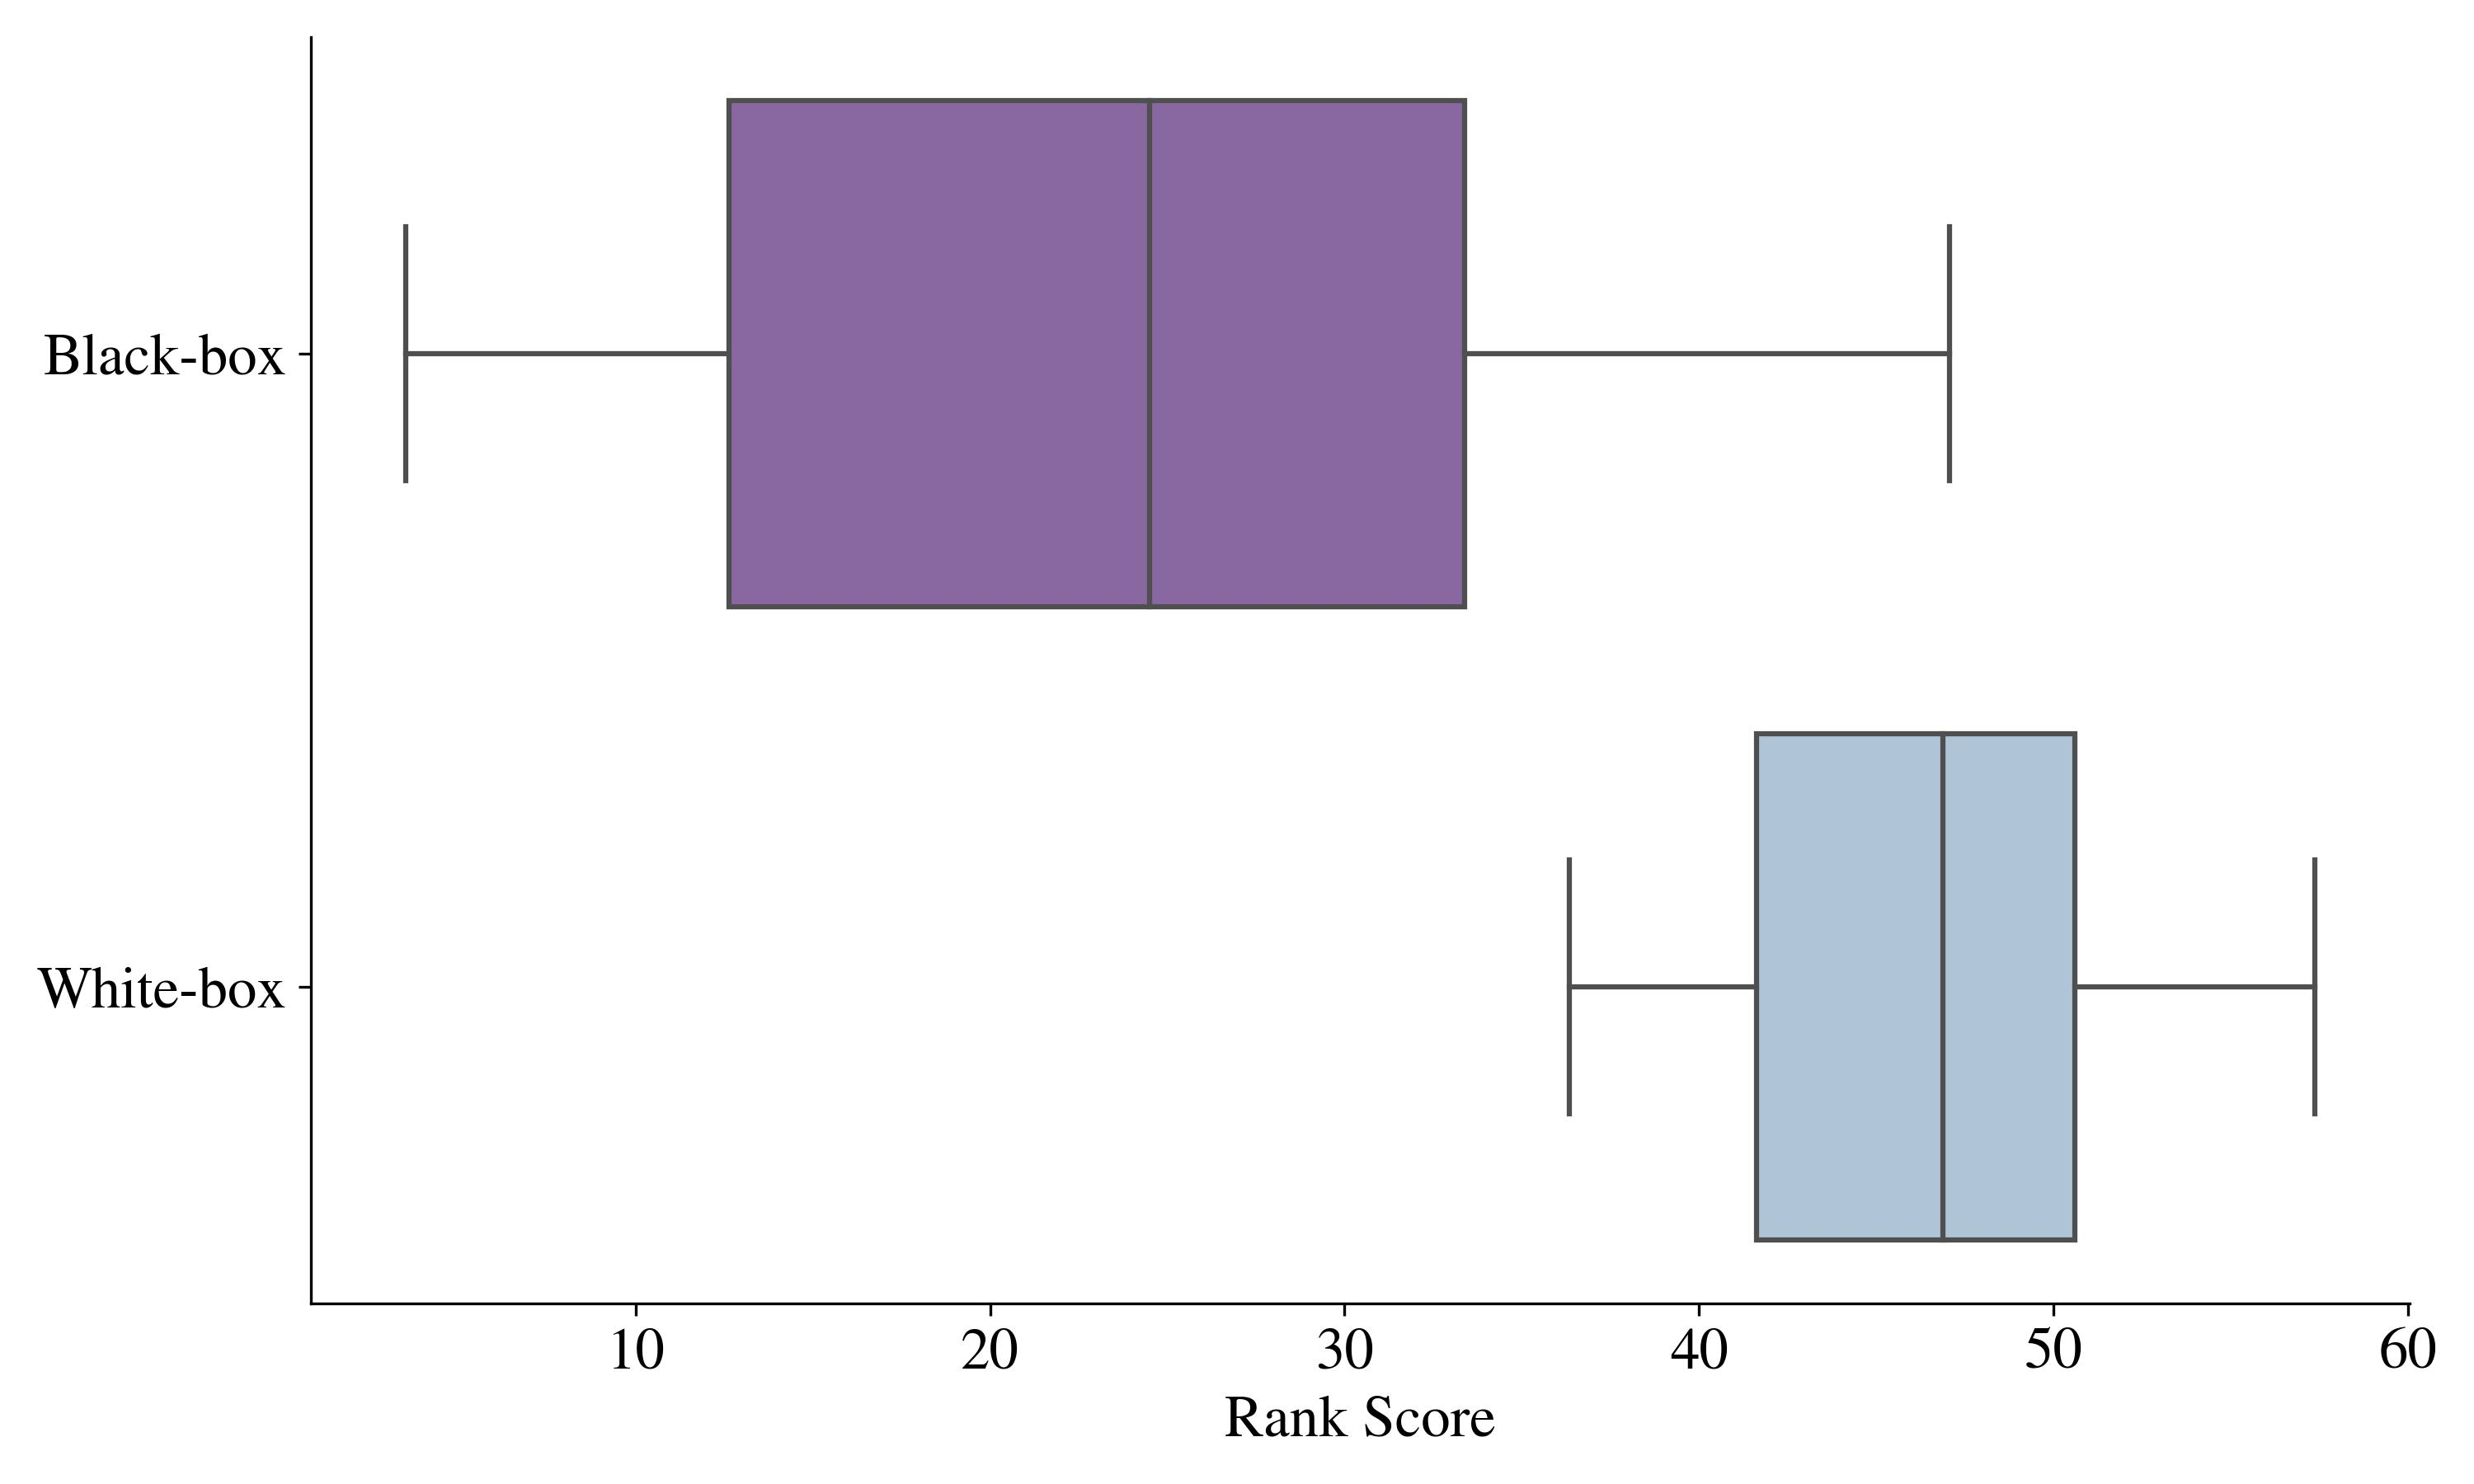
\includegraphics[width=140mm]{Figures/AVG_Rank_score_Distribution_BB_WB.jpg}
    \centering{\begin{source}Author's results in Python\end{source}}\vspace{-1em}
\end{figure}


The optimal threshold distribution for each base model is presented in \autoref{fig:thresdist}. We can observe an outlier in KNN having a threshold value of 1, which explains the F1 score outlier found previously in \autoref{fig:f1dist}.
\begin{figure}[H]
\centering
\caption{Threshold Distribution}\vspace{0.5em}
\label{fig:thresdist}\
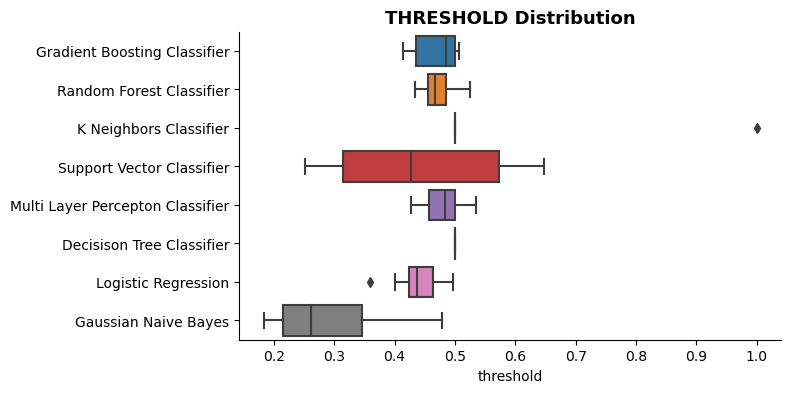
\includegraphics[width=140mm]{Figures/Threshold_Distribution.jpg}
\centering{\begin{source}Author's results in Python\end{source}}\vspace{-1em}
\end{figure}

In order to obtain a better insight into the distribution of optimal thresholds, the outlier in KNN is excluded, resulting in the threshold distribution depicted in \autoref{fig:thresdistclean}. The optimal threshold values are mostly distributed below 0.5, indicating that the models are generally more conservative. The most conservative model is Gaussian Naive Bayes, which has a median threshold value around 0.25.
\begin{figure}[H]
\centering
\caption{Threshold Distribution - \textit{without outlier}}\vspace{0.5em}
\label{fig:thresdistclean}\
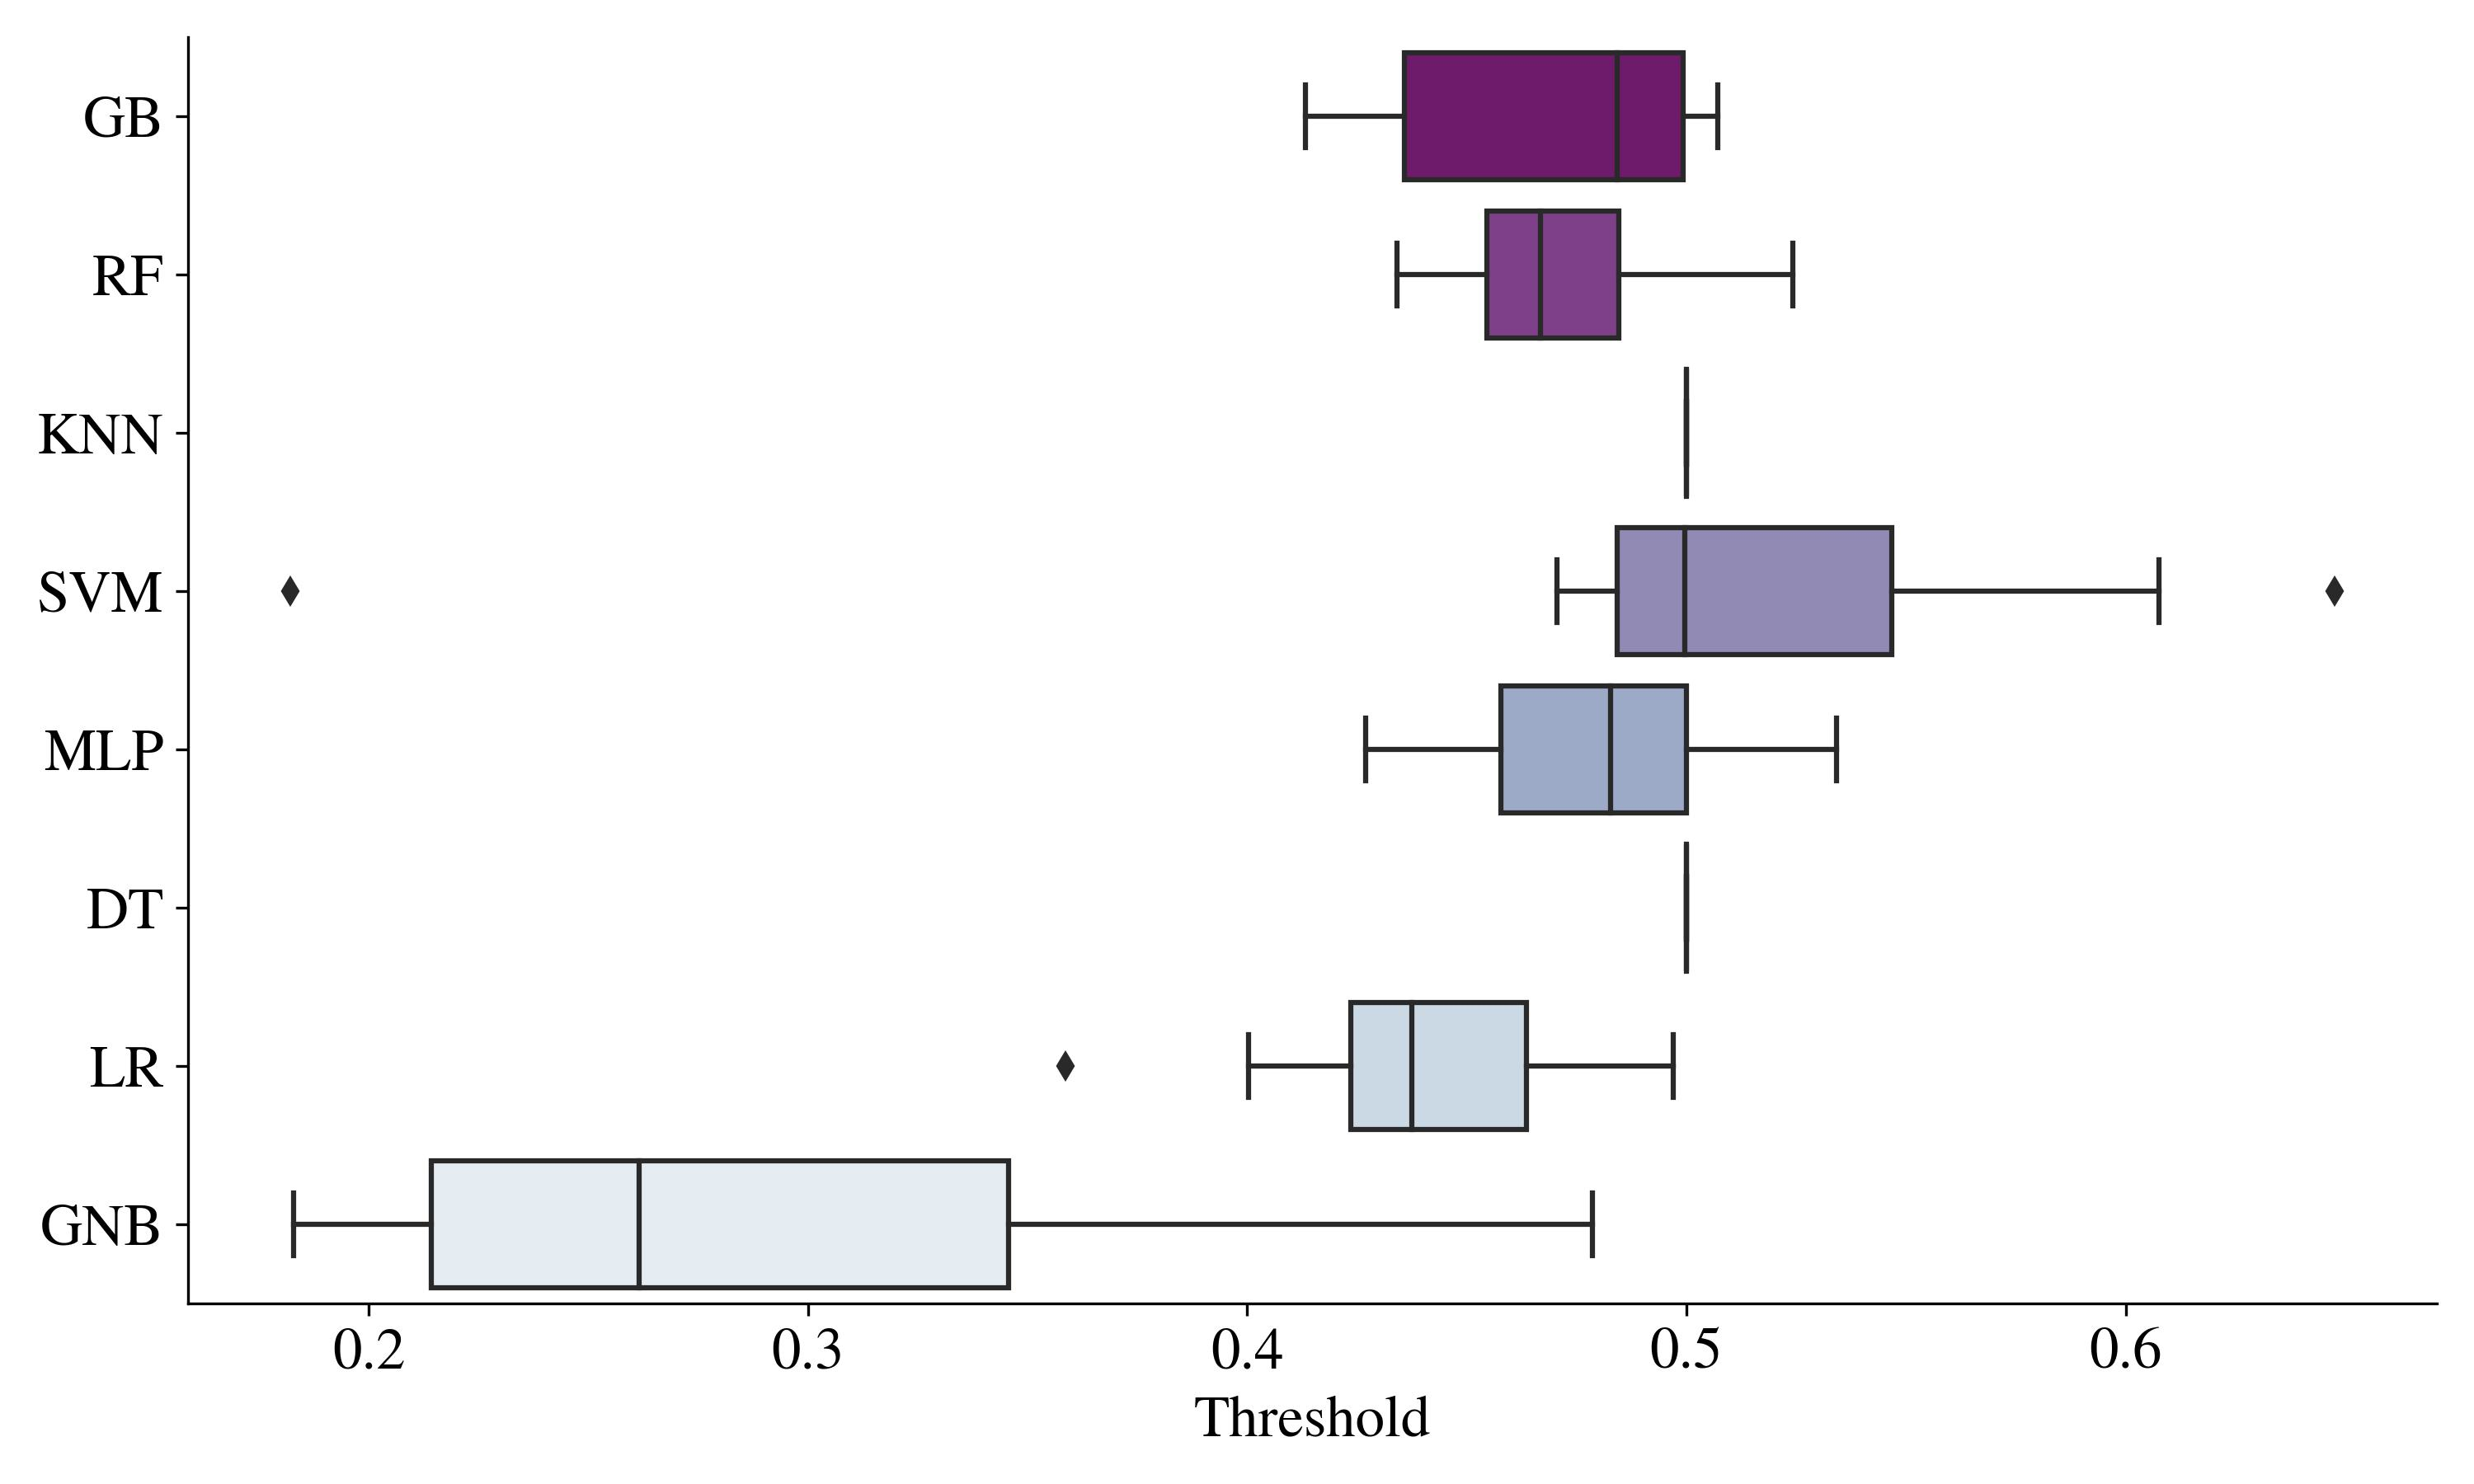
\includegraphics[width=140mm]{Figures/Threshold_wo_outliers_Distribution.jpg}
\centering{\begin{source}Author's results in Python\end{source}}\vspace{-1em}
\end{figure}




Upon examining the execution time of each model, it can be observed that the transparent and non-complex models such as Logistic Regression, Gaussian Naive Bayes, or even Decision Tree, which take around only 1 minute to optimize themselves, also perform poorly, as already inspected in \autoref{fig:f1distclean}.
Conversely, the most time-consuming models are undoubtedly the Neural Network models, which take around 30 minutes to optimize themselves. Other time-consuming models include Gradient Boosting and Support Vector Machine, which take around 13 and 11 minutes to optimize themselves, respectively.
This finding suggests that longer execution time does not necessarily lead to better performance, as the Neural Network models are significantly outperformed by several other models.
\begin{figure}[H]
\centering
\caption{Execution Time Distribution}\vspace{0.5em}
\label{fig:timedist}\
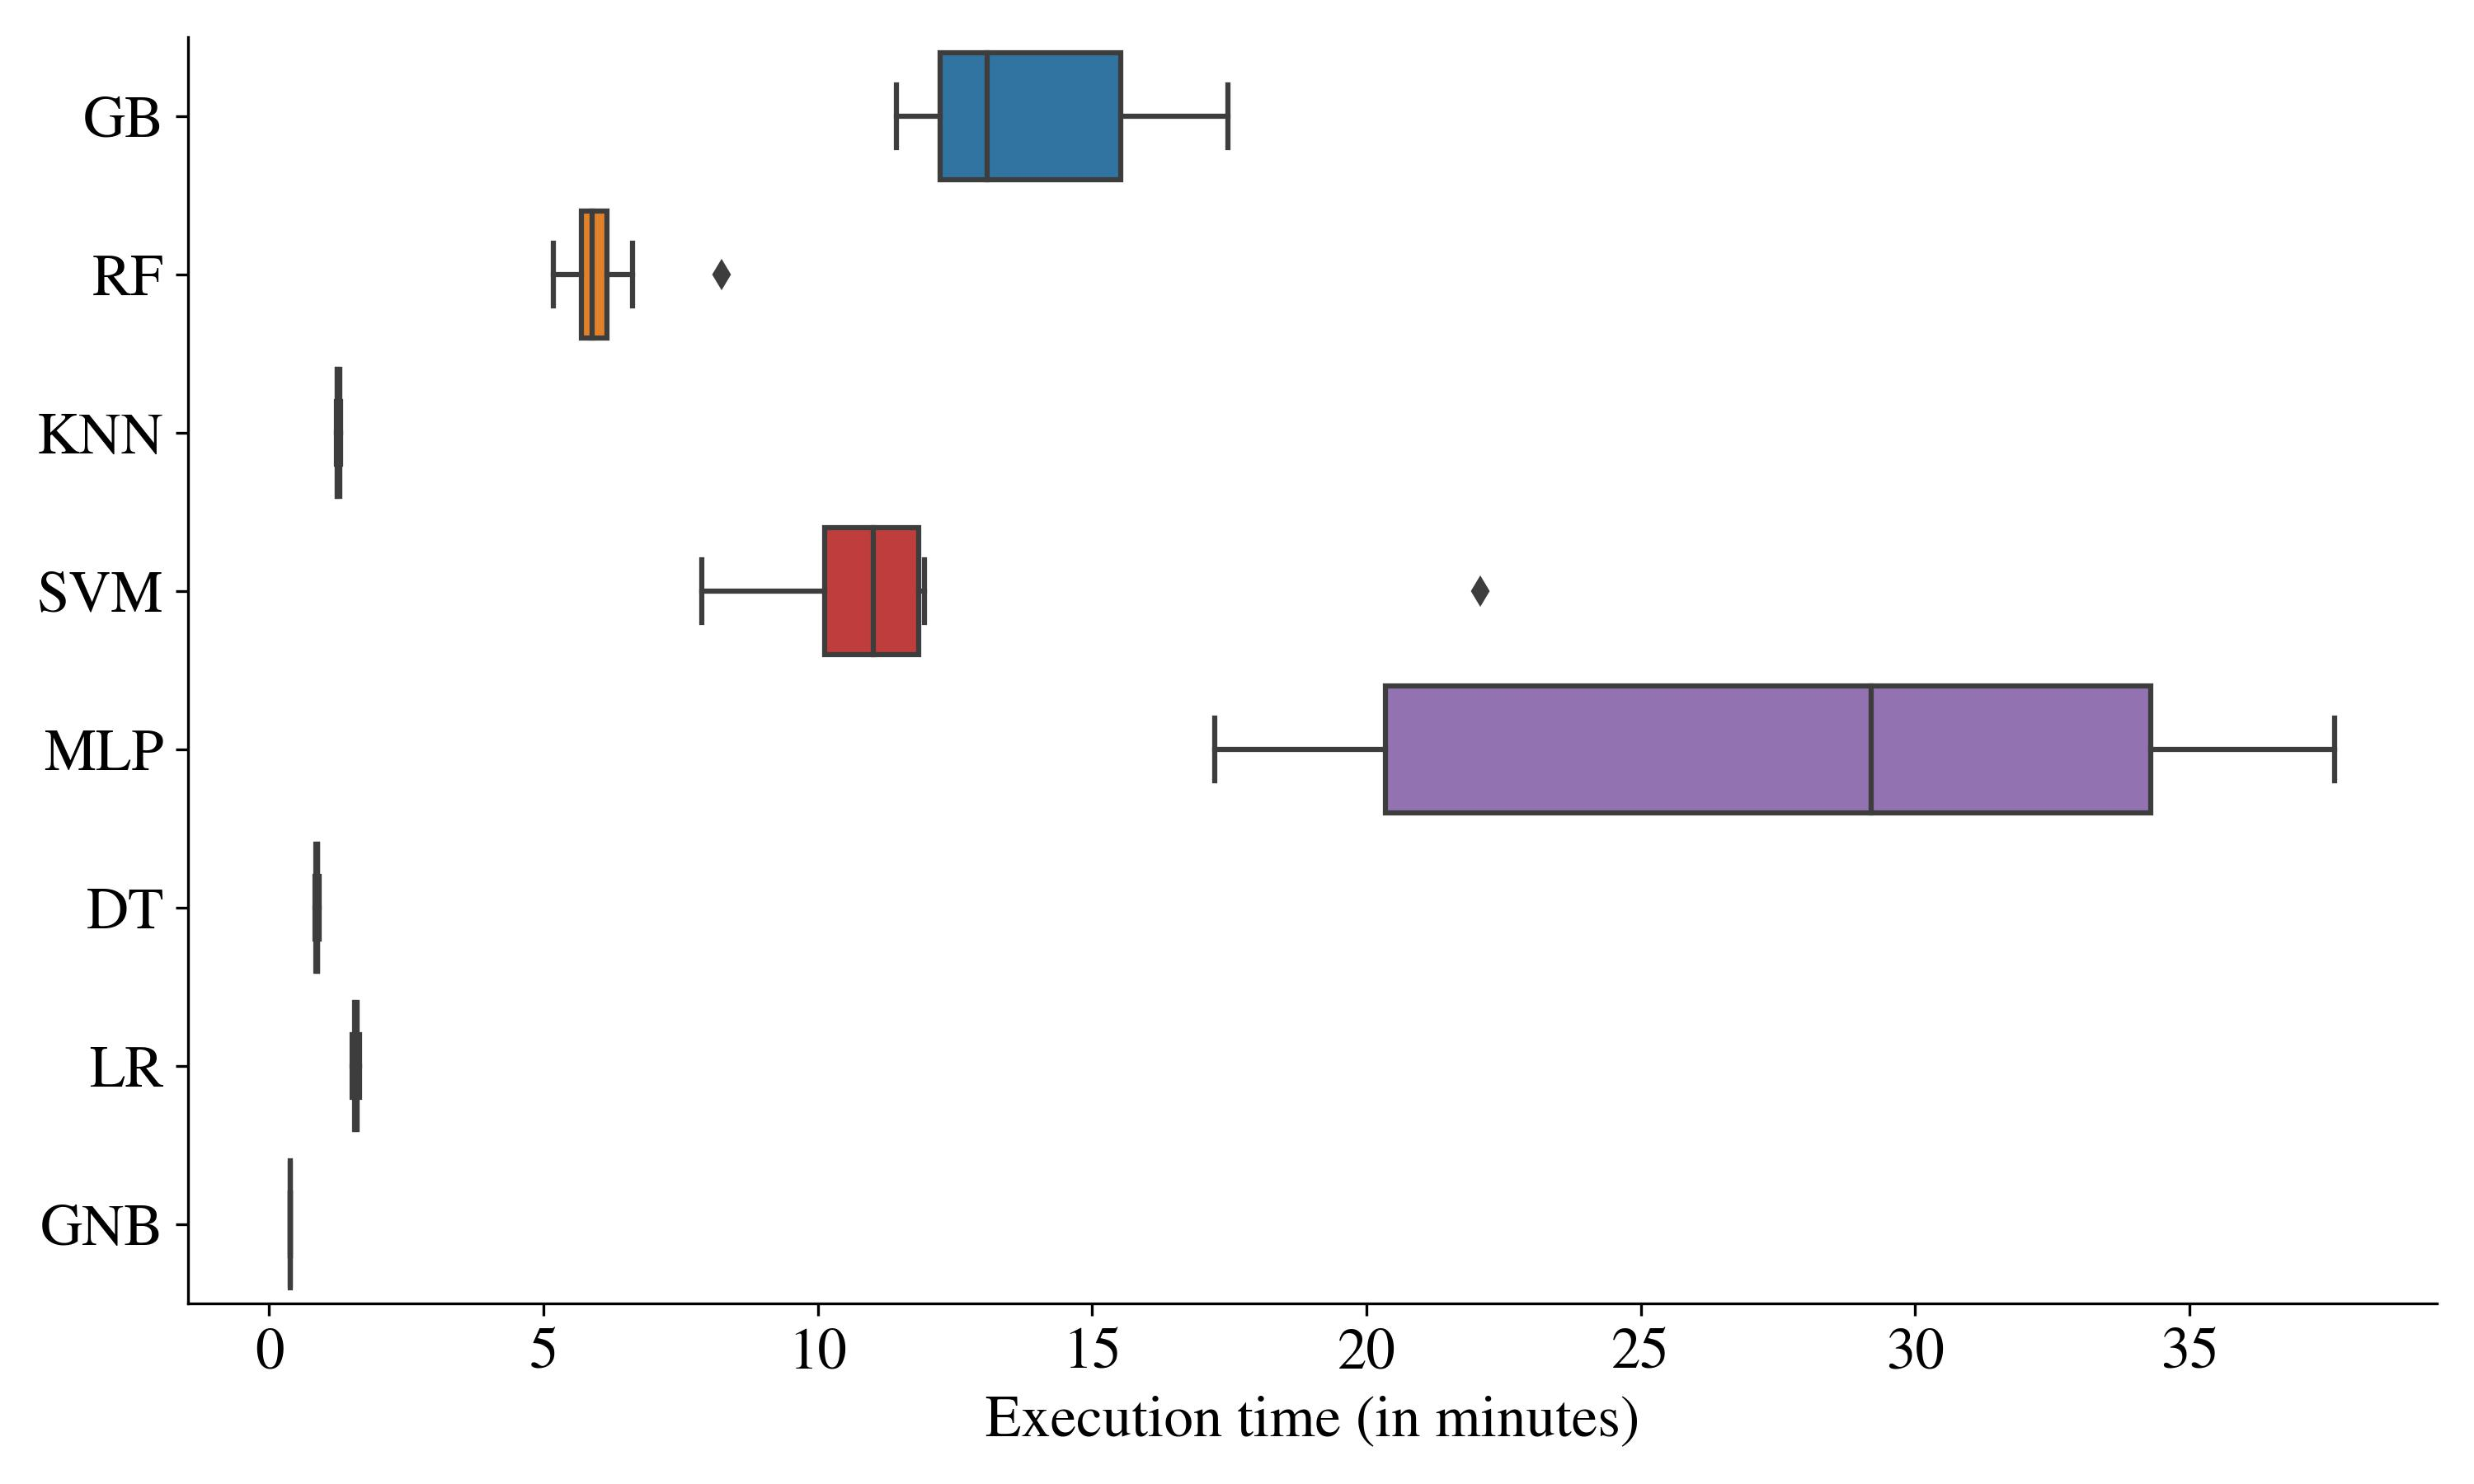
\includegraphics[width=140mm]{Figures/EXECUTION_TIME_Distribution.jpg}
\centering{\begin{source}Author's results in Python\end{source}}\vspace{-1em}
\end{figure}
We can inspect the execution time from another perspective as shown in \autoref{fig:timedistbbwb}.
It can be observed that black--box models take a significant amount of time ot opimize than the white--box models which is given due to the complexity of the black--box models.
Further we can notice that some of the black--box models took only few minutes to optimized themselves. This corresponds to KNN models and it can be attributed to the small sample size as of data set as well as lower data set dimensionality (i.e., low number of features) and further given the lower number of $k$ neighbors (which is constrained to 10 at most as depicted in \autoref{tab:knnspace}).
\begin{figure}[H]
    \centering
    \caption{Execution Time Distribution (Black--box/White--box dimension)}\vspace{0.5em}
    \label{fig:timedistbbwb}\
    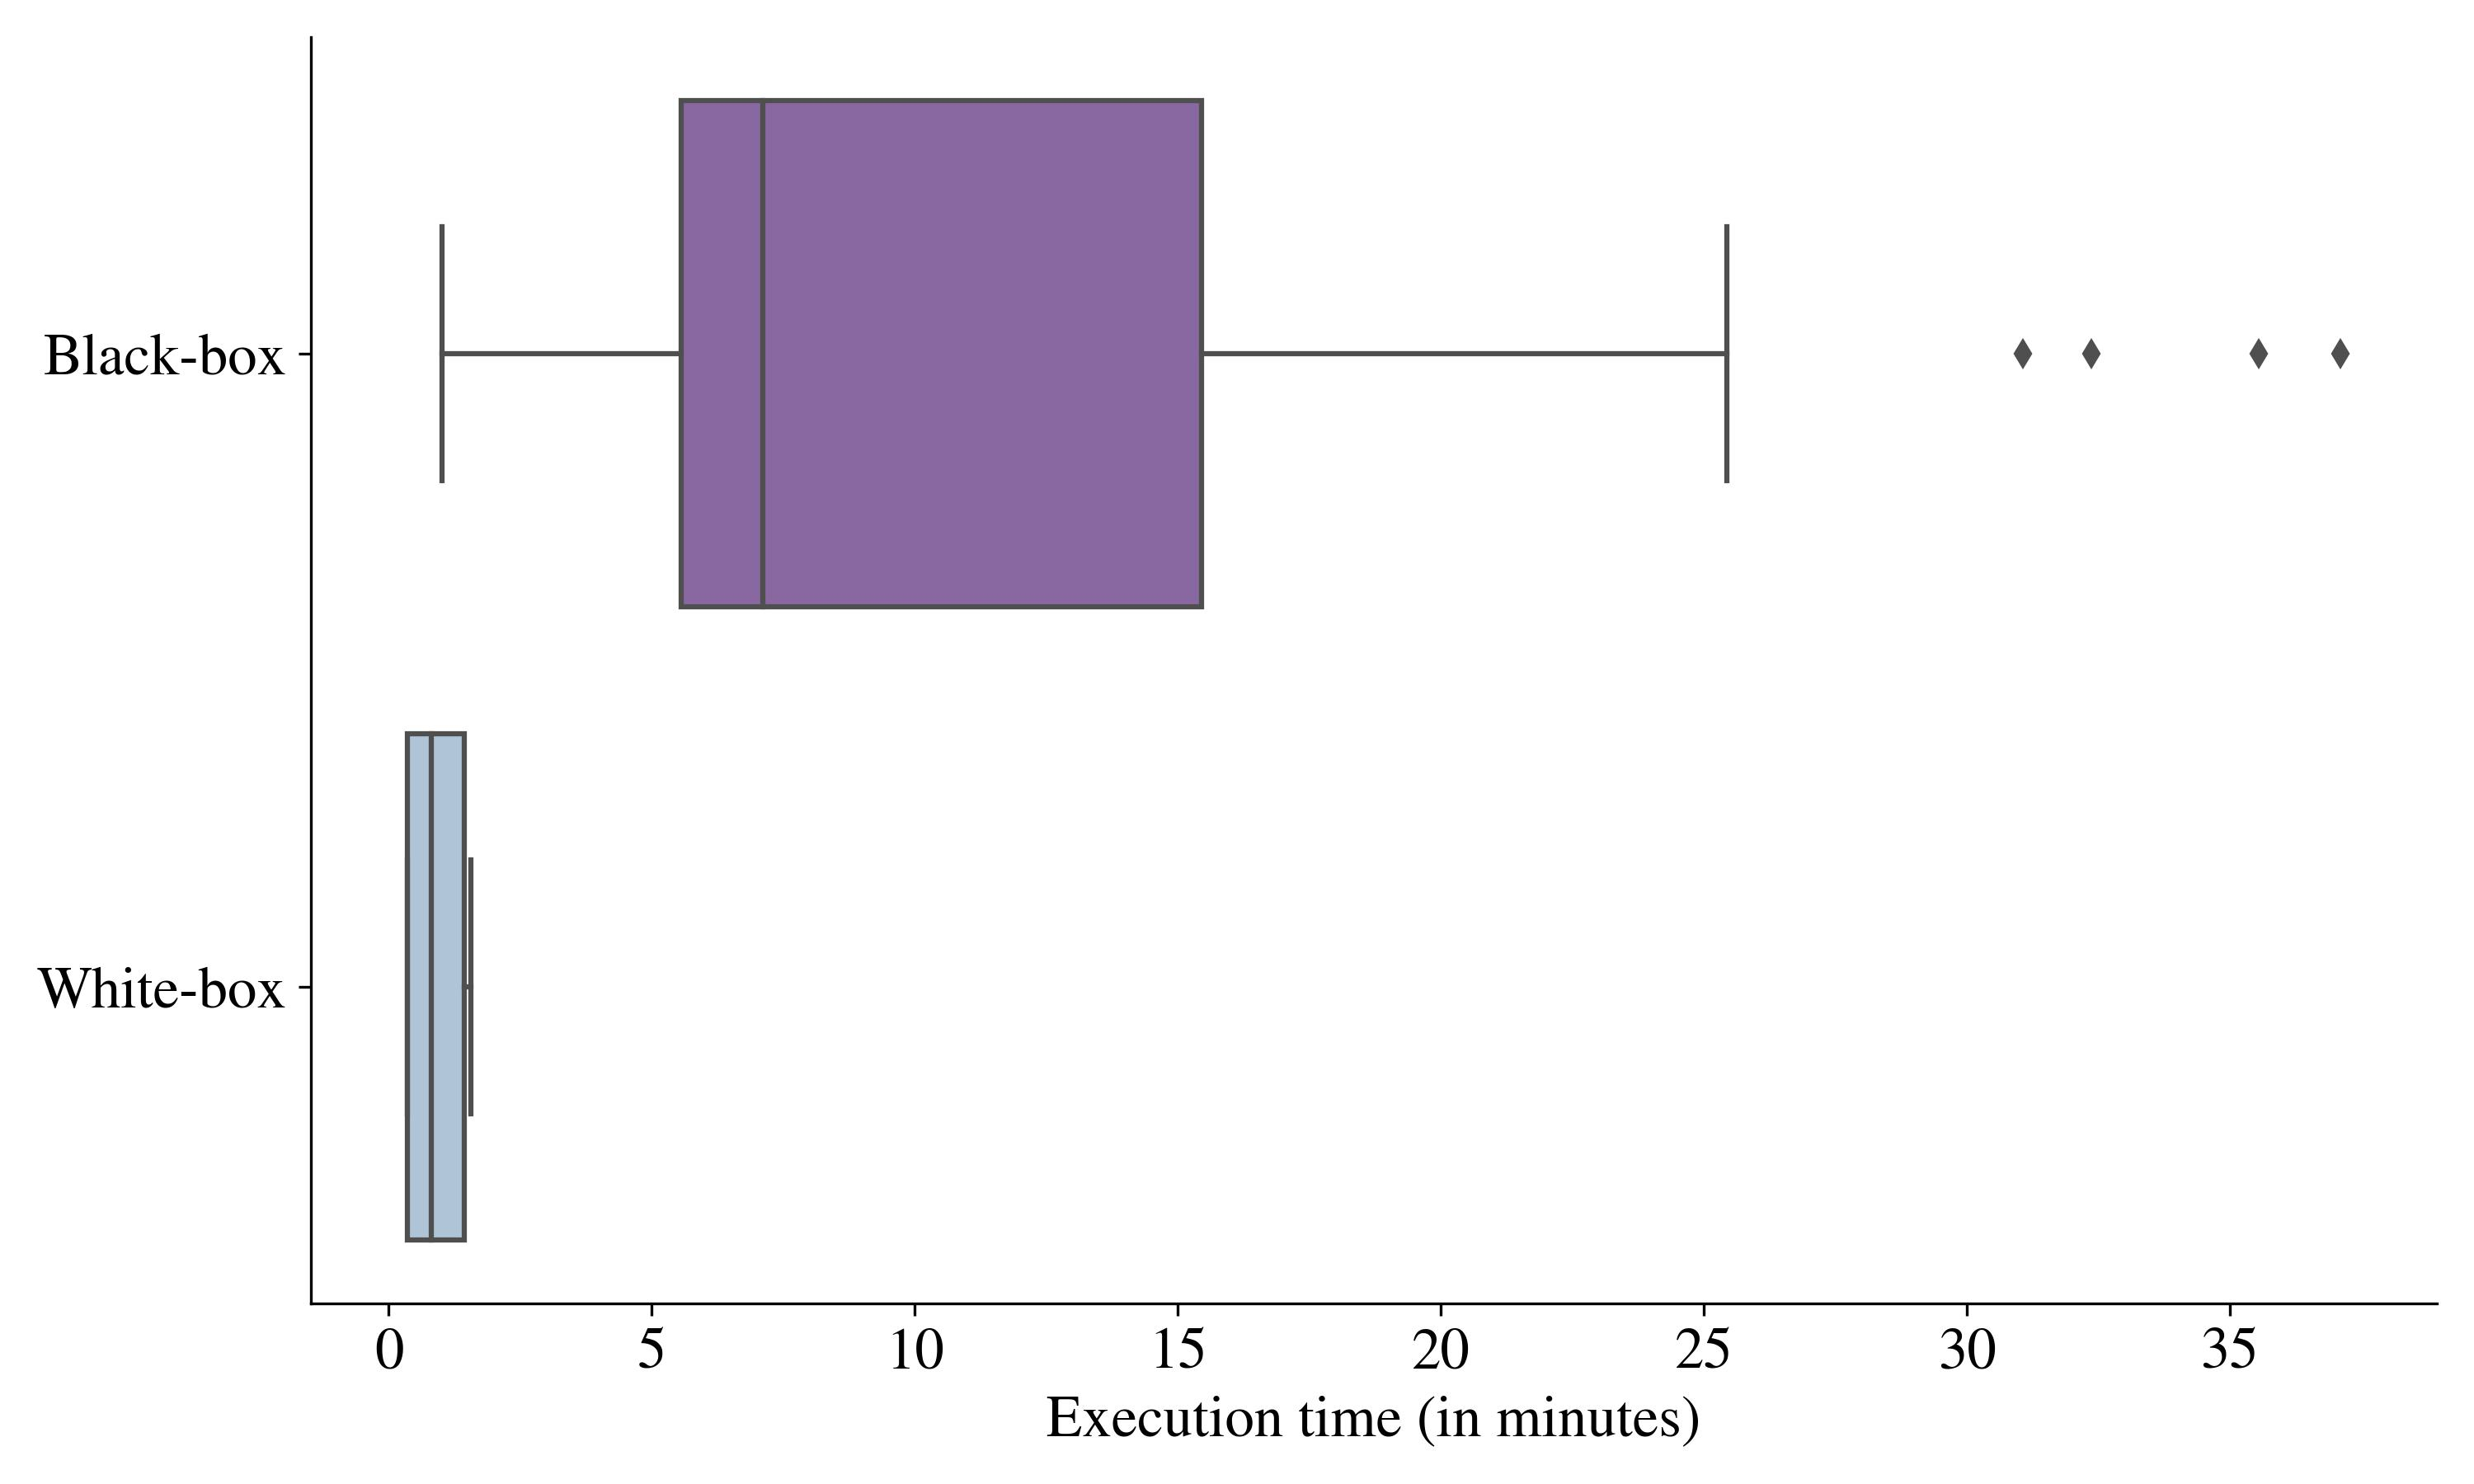
\includegraphics[width=140mm]{Figures/EXECUTION_TIME_Distribution_BB_WB.jpg}
    \centering{\begin{source}Author's results in Python\end{source}}\vspace{-1em}
\end{figure}


The execution time and the F1 score are inspected together using a scatterplot, as shown in \autoref{fig:scattertime}. 
A cluster of non-complex and transparent models, such as Logistic Regression, Gaussian Naive Bayes, and Decision Tree, can be observed around the vertical line near 0 execution time. These models are quick to optimize, but their F1 scores are generally low.
Further, their variance in execution time is quite low, regardless of the feature subset they are optimized on.
On the other hand, the Neural Network models always perform poorly, regardless of the length of the execution time. Furthermore, the variance of the F1 scores is quite low for these models, indicating that the execution time does not have a significant impact on the F1 score in the case of Neural Networks.

\begin{figure}[H]
\centering
\caption{Execution Time vs. F1 Scatterplot - \textit{without outlier}}\vspace{0.5em}
\label{fig:scattertime}\
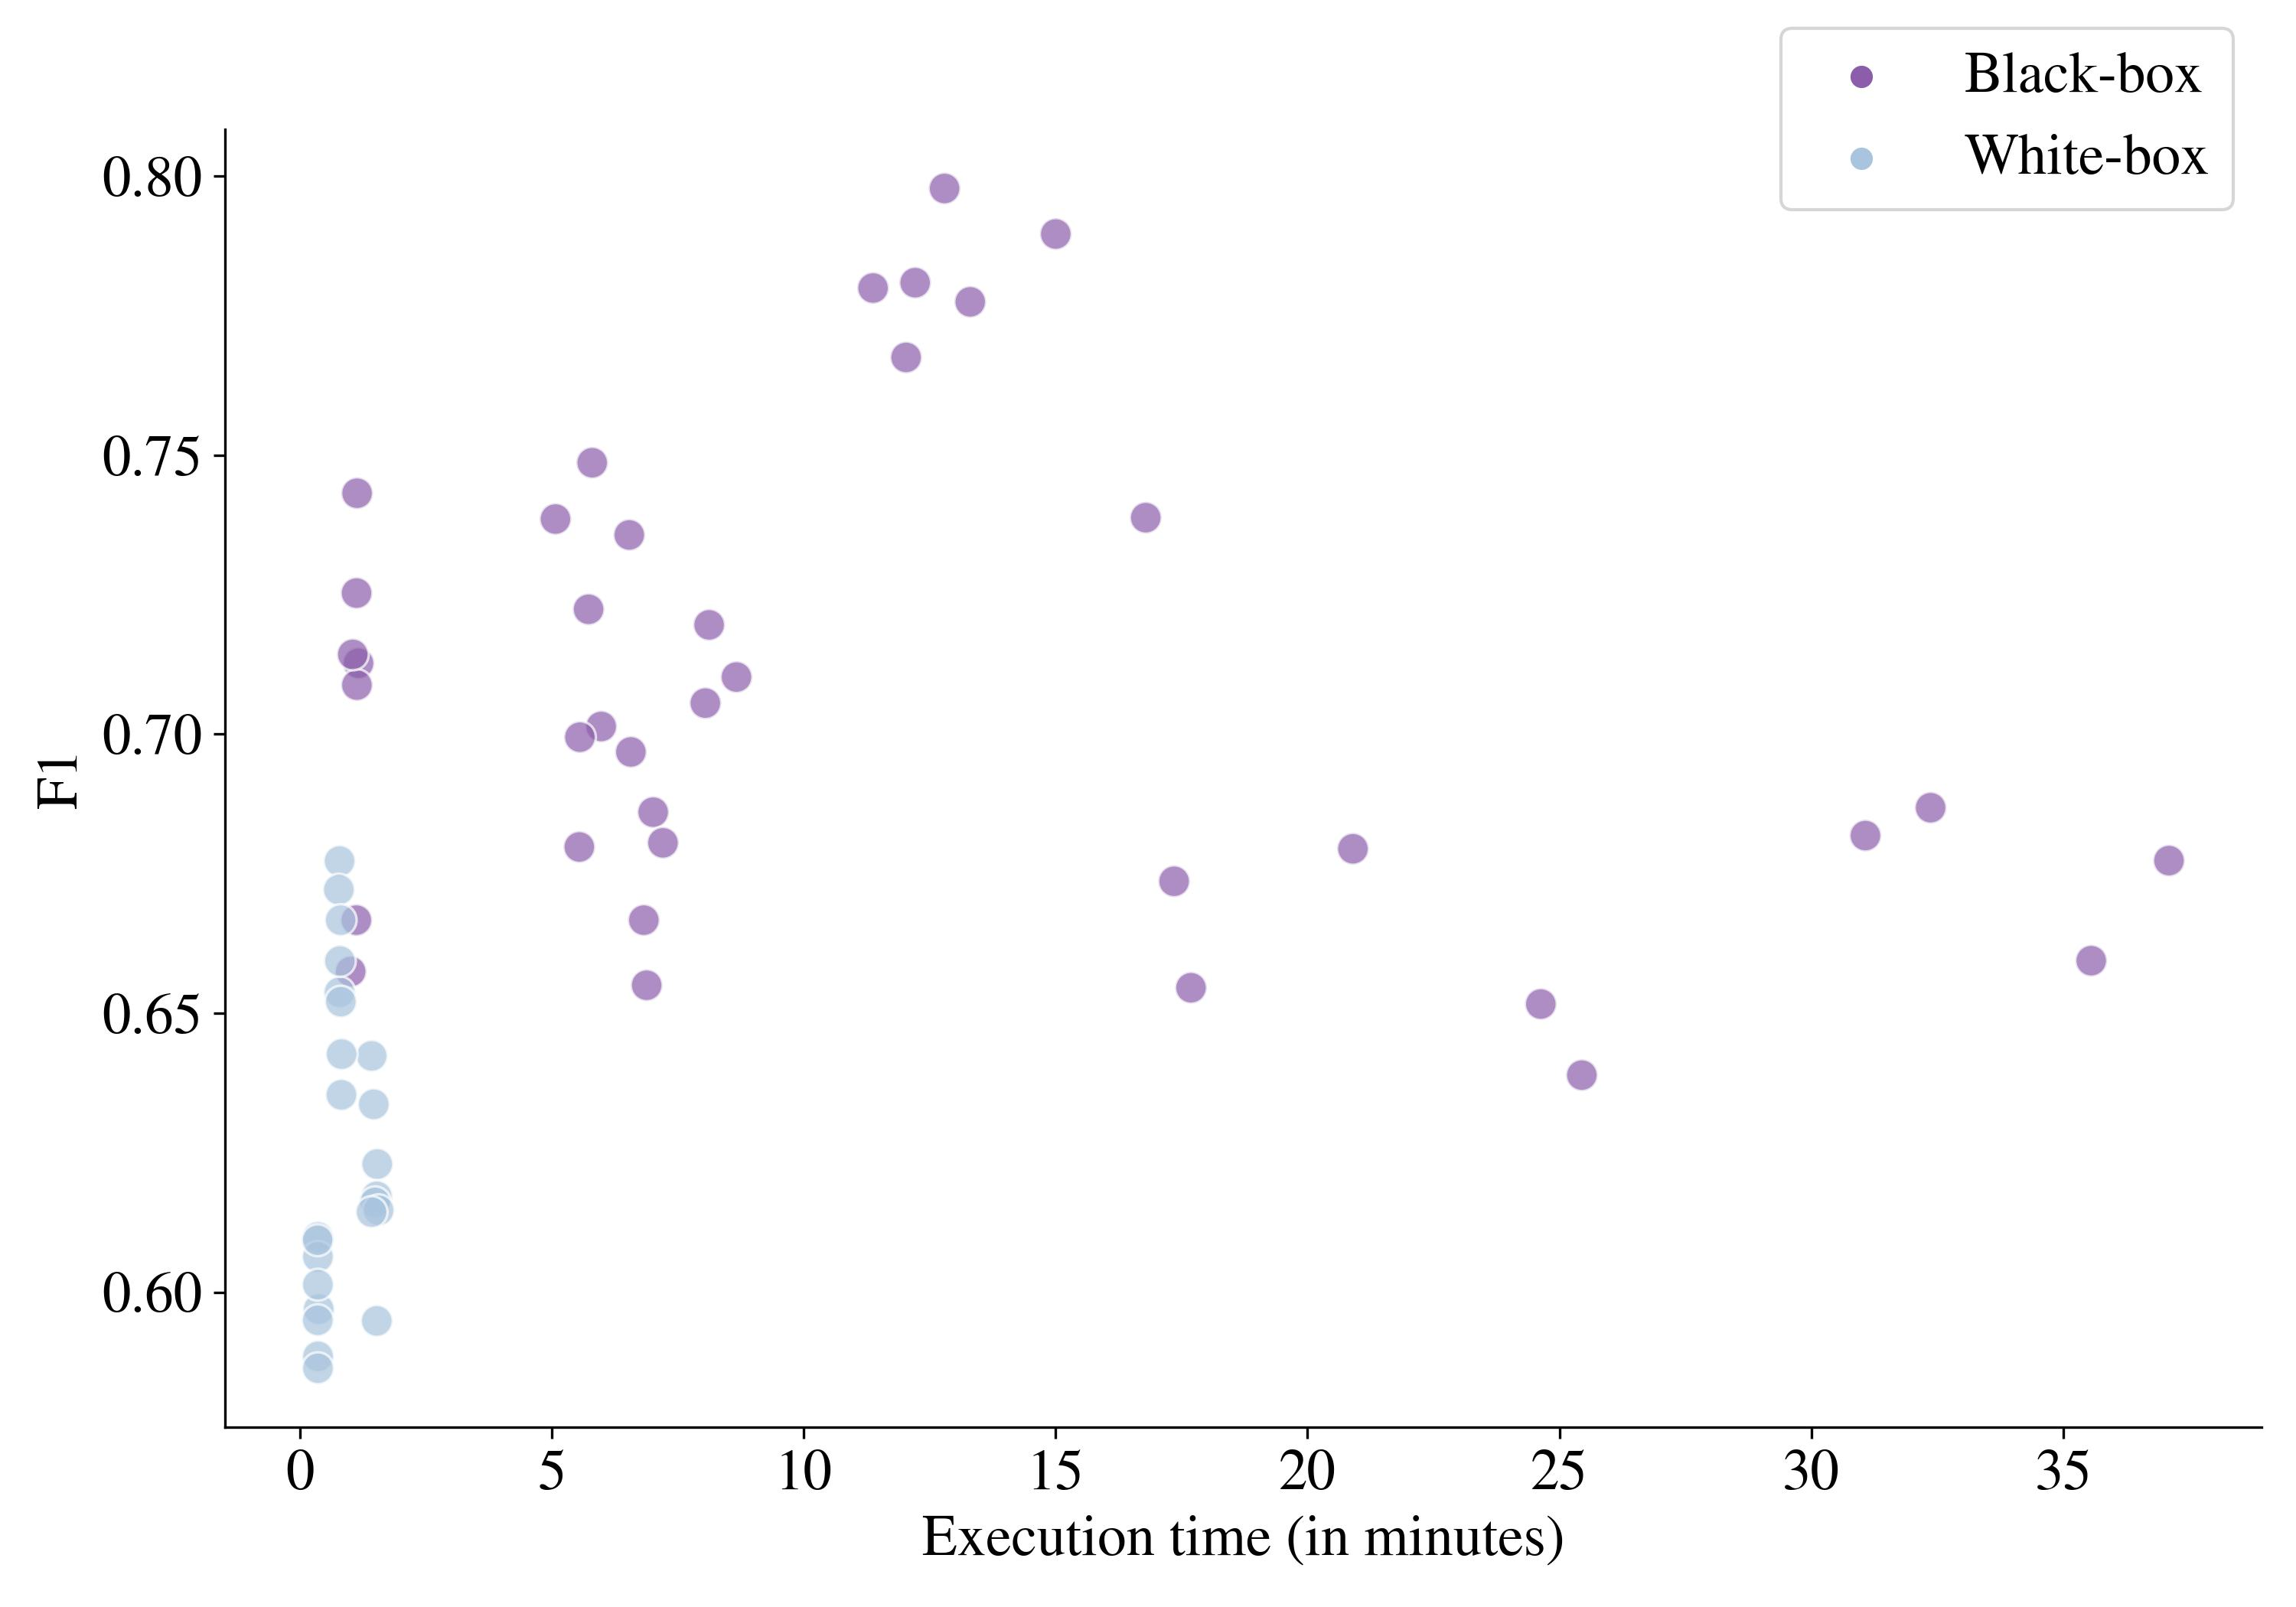
\includegraphics[width=140mm]{Figures/Scatterplot_execution_time_F1_wo_outliers.jpg}
\centering{\begin{source}Author's results in Python\end{source}}\vspace{-1em}
\end{figure}
Such separation of of the black--box and white--box models is more evident from \autoref{fig:scattertimebbwb} where the white--box models points are light blue-colored and the black--box models are purple-colored.
While the score of white--box models seems to be constant regardless the execution time length, the points of black--box models are more dispersed across the execution time--F1 score dimension.

\begin{figure}[H]
    \centering
    \caption{Execution Time vs. F1 Scatterplot (Black--box/White--box dimension) - \textit{without outlier}}\vspace{0.5em}
    \label{fig:scattertimebbwb}\
    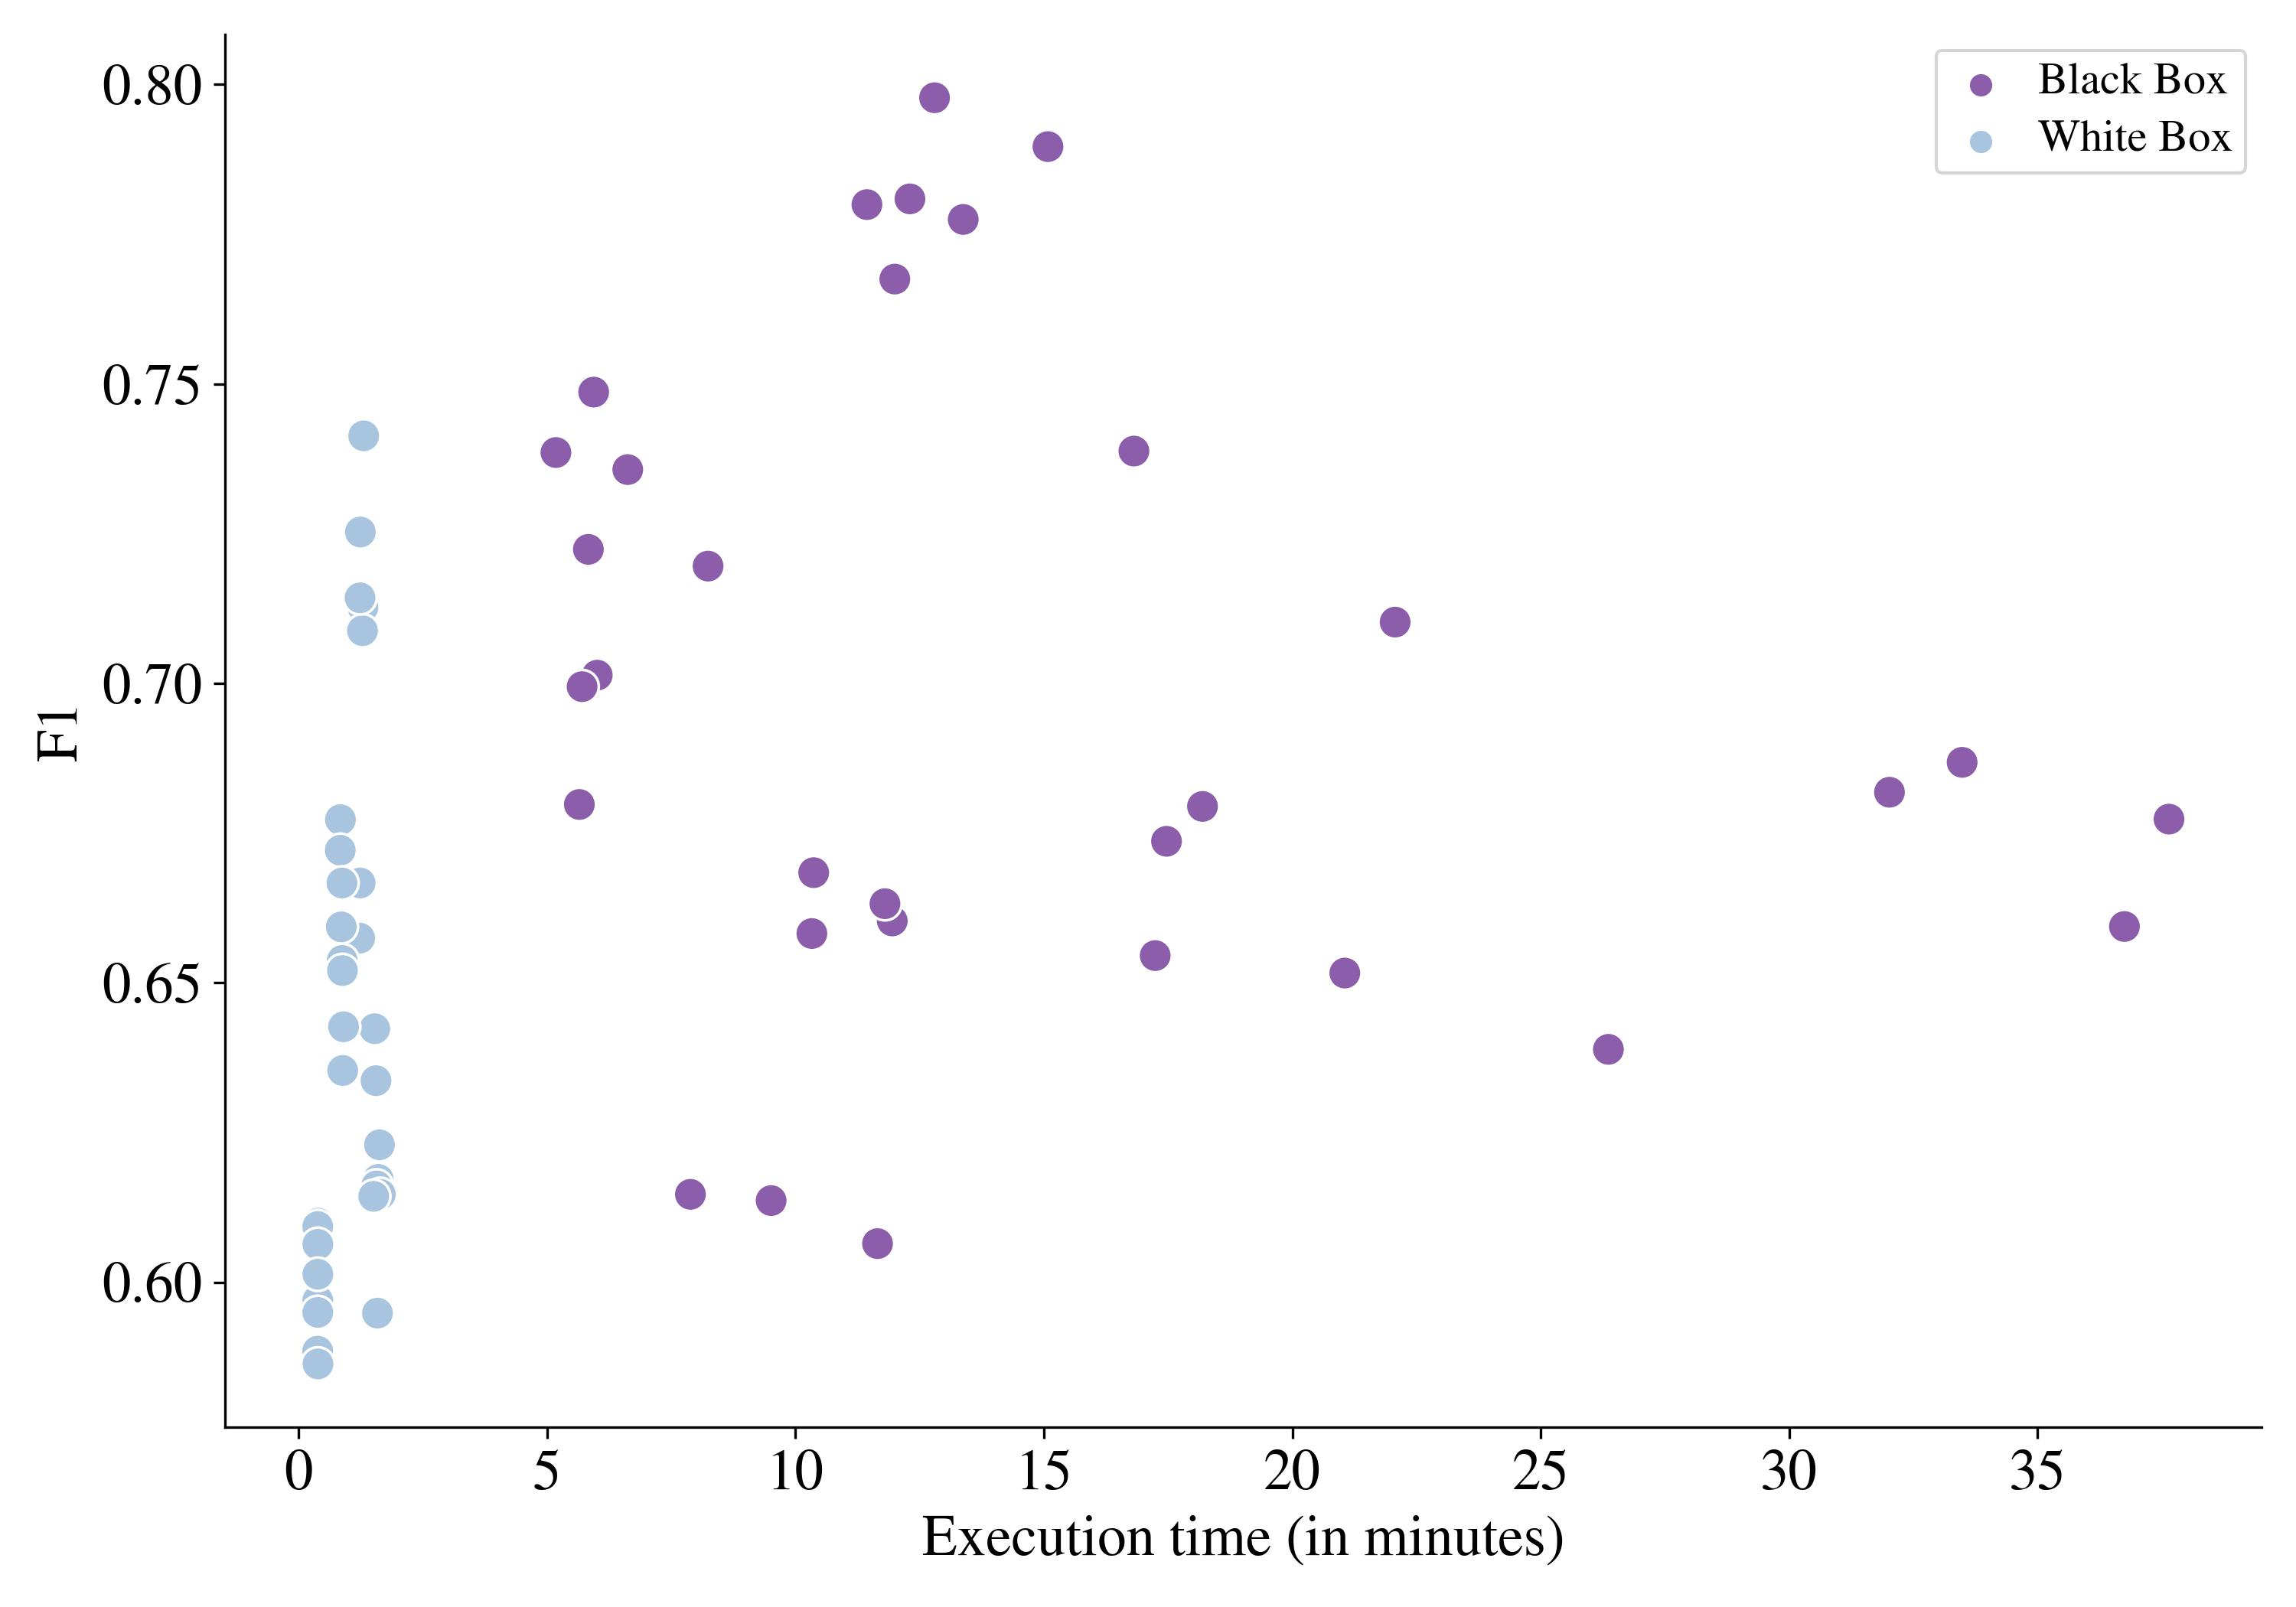
\includegraphics[width=140mm]{Figures/Scatterplot_execution_time_F1_wo_outliers_BB_WB.jpg}
    \centering{\begin{source}Author's results in Python\end{source}}\vspace{-1em}
\end{figure}


To summarize this subsection, the best and final model is the \textbf{Gradient Boosting Classifier} which was optimized on the subset of features selected by \textbf{MLP} - both the model information and its final hyperparameters' values are described in \autoref{tab:finalmodelinfo}. Such model is then used in the next modelling steps, including the recalibration, evaluation and deployment.
\begin{table}[H]
    \small
    \setlength{\tabcolsep}{8pt}
    \renewcommand{\arraystretch}{1.3}
    \centering
    \caption{Final Model Information}\label{tab:finalmodelinfo}
    \begin{tabular}{>{\raggedleft\arraybackslash}p{0.20\linewidth}|p{0.65\linewidth}}
    \toprule
    \midrule
    \textbf{Final Model} & Gradient Boosting \\
    \midrule
    \textbf{FS Model} & Multi--Layer Percepton \\
    \midrule
    \textbf{Final Features} &
    MORTDUE, VALUE, JOB, YOJ, DEROG, DELINQ, CLAGE, NINQ, CLNO, DEBTINC \\
    \midrule
    \textbf{Threshold} & 0.4955 \\
    \midrule
    \textbf{F1} & 0.7809 \\
    \midrule
    \textit{\# estimators} & 1,000 \\
    \midrule
    \textit{Criterion} & Friedman MSE \\
    \midrule
    \textit{Max depth} & 10 \\
    \midrule
    \textit{Max features} & 1 \\
    \midrule
    \textit{Loss} & Log loss \\
    \midrule
    \textit{Learning rate} & 0.0150 \\
    \midrule
    \bottomrule
    \end{tabular}
    \vspace{0.5em}
    
    \centering{\begin{source}Author's results in Python\end{source}}\vspace{-0.5em}
\end{table}

\newpage
\subsection{Model Recalibration}
\label{subsec:modelrecal}

In order to ensure that the final model performs well on unseen data, it is common practice to employ the recalibration approach, which involves retraining the model on both the training and validation sets.
By doing so, the sample size used for training is increased. As such, the retraining (or so called recalibration) model lead (or are expected to lead) to markedly improved model performance \citep{de2023predicting}.
The recalibrated model is then used to evaluate the performance of the final model on the test set, which is the ultimate measure of a model's performance.

In addition to recalibrating the final model, it is crucial to recalibrate the threshold value for assigning class labels based on predicted probabilities. The optimal threshold value can be determined using the training and validation sets. Such threshold is recalibrated based on the training and validation set.
In this thesis, the optimal threshold value is found to be \textbf{0.45109}, which is then used for evaluating the final model's performance on the test set.
By recalibrating the threshold value, the model's performance is further improved, resulting in more accurate predictions. After the recalibration process, we can observe that the model is more conservative as its optimal classification threshold has decreased. The impact on the model's performance is further assessed in \autoref{subsec:modelperformance}.

Moreover, the recalibration process helps to mitigate overfitting issues, which occur when the model is only trained on the training set.
By incorporating the validation set into the training process, the recalibrated model can better generalize to new data and improve its overall performance on the test set.
The inclusion of the validation set during the recalibration process does not cause any data leakage issues since this set was already used during model selection to evaluate each model's performance.
Therefore, using the validation data for recalibration is a sound practice that helps to ensure the reliability and accuracy of the final model.

\newpage
\section{Model Evaluation}
After recalibrating the model and threshold, the final step in evaluating the model's performance is to test it on previously unseen data, specifically the test set.
This evaluation is critical to determine whether the model can generalize well to new data beyond the training, feature selection, and model selection phases.
During the evaluation, the recalibrated classification threshold of 0.45109, determined in the model recalibration process, is also used.
\subsection{Model Performance Assessment}
\label{subsec:modelperformance}



In \autoref{fig:confmat}, the confusion matrix for the final model, based on the test set and using the recalibrated threshold, is presented. The matrix shows that the model is generalizing well, having correctly predicted 145 defaults and misclassified only 33 defaults and further, correctly predicted 683 non--defaults and misclassified only 33 non--defaults. Such a result indicates that the model is a good fit for the data and can provide useful predictions for the problem at hand.

\begin{figure}[H]
\centering
\caption{Confusion Matrix}\vspace{0.5em}
\label{fig:confmat}\
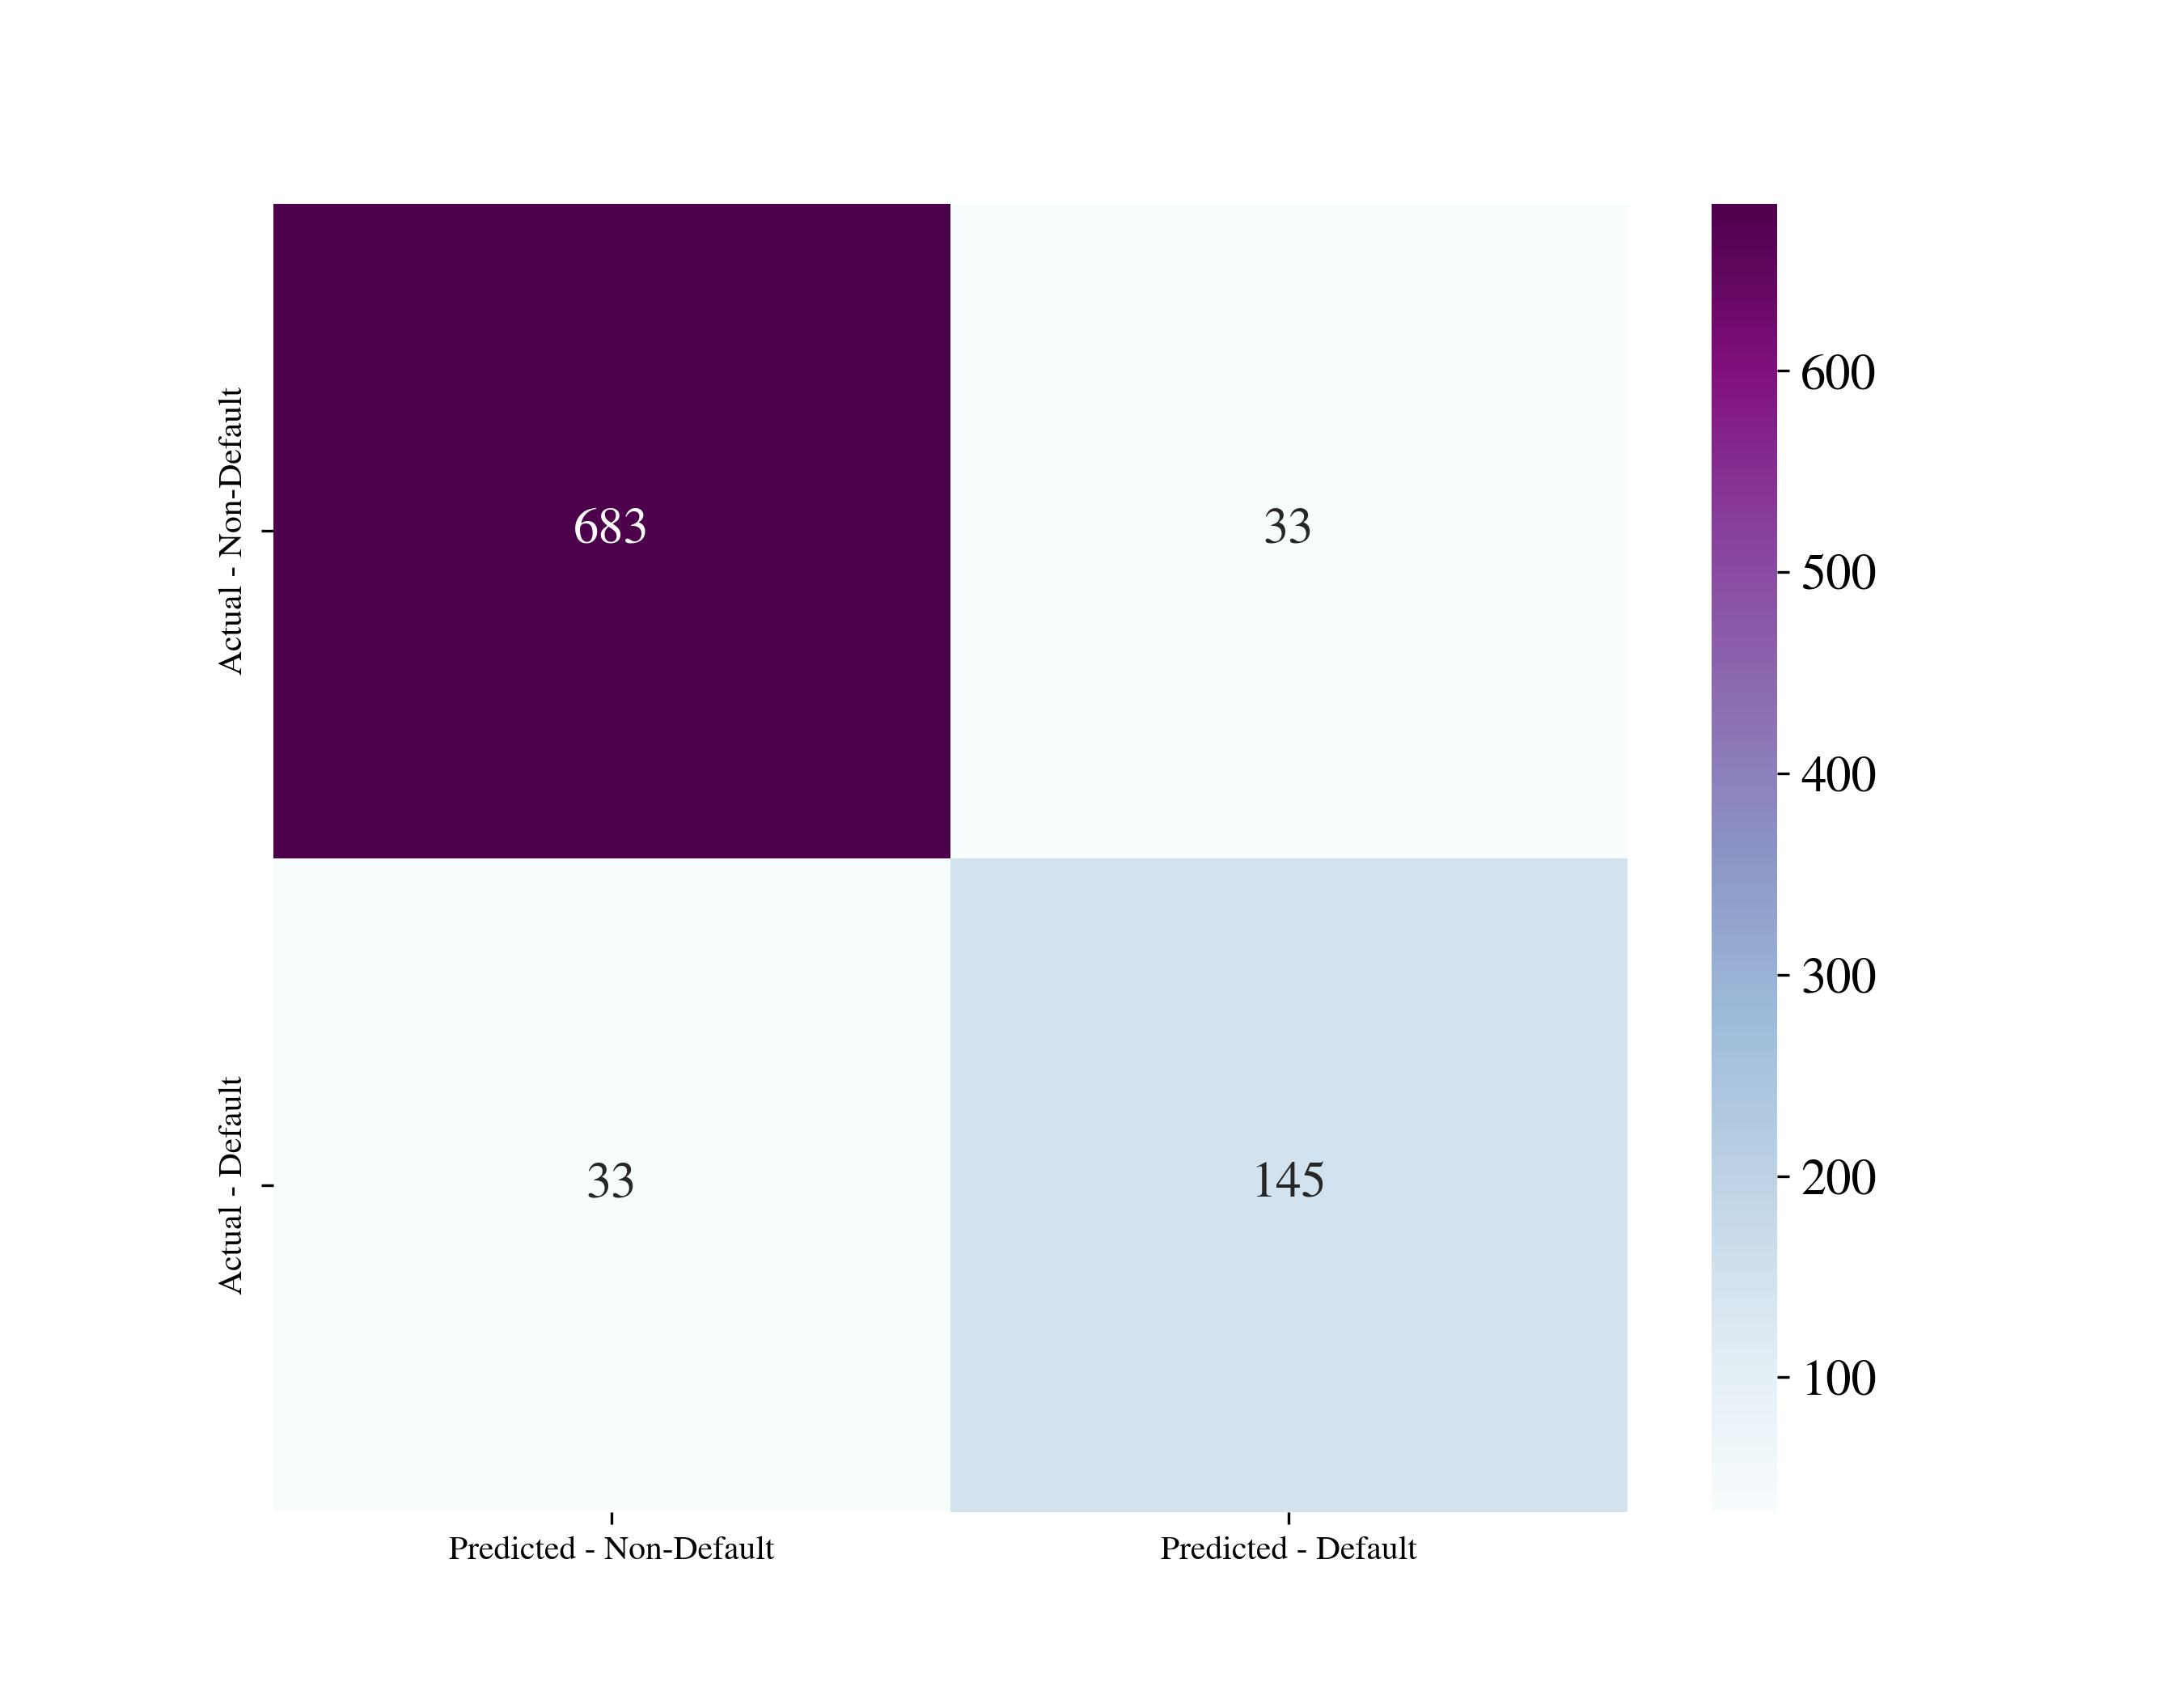
\includegraphics[width=130mm]{Figures/Confusion_Matrix.jpg}
\centering{\begin{source}Author's results in Python\end{source}}\vspace{-1em}
\end{figure}

In order to obtain a better understanding of the model's performance on previously unseen data, we computed several metrics that were used during the model selection process.
These metrics are presented in \autoref{tab:metricseval}. The results indicate that the model performs well on the unseen data, with most of the scores metrics around 80 \% to 90 \%.
Furthermore, the loss metrics are relatively low, indicating that the model can effectively distinguish between defaults and non-defaults.
Overall, these results suggest that the model is performing well and is suitable for predicting defaults.
The results suggest that the model has a good balance between correctly identifying defaults and non-defaults, as well as minimizing false positives and false negatives. This further confirms the model's ability to accurately predict defaults.

\begin{table}[H]
    \small
    \setlength{\tabcolsep}{8pt}
    \renewcommand{\arraystretch}{1.3}
    \centering
        \caption[Metrics Evaluation]{Metrics Evaluation}\label{tab:metricseval}
        \begin{tabular}{@{} r r @{\hspace{1cm}} l @{}}
    \toprule
    \textbf{Metric} & \textbf{Value}\\
    \midrule
    \hline
    F1 & 0.8146 \\ 
    Precision & 0.8146 \\ 
    Recall & 0.8146 \\ 
    Accuracy & 0.9262 \\ 
    AUC & 0.9564 \\ 
    Somers' D & 0.9128 \\ 
    KS & 0.7915 \\ 
    MCC & 0.7685 \\ 
    Brier Score Loss & 0.0594 \\
    Log Loss & 0.2163 \\
    \hline
    \bottomrule
    \end{tabular}
    \vspace{0.35em}

        \centering{\begin{source}Author's results in Python\end{source}}\vspace{-1em}
\end{table}

The following \autoref{tab:recab} shows the impact of recalibration on the model's performance metrics. $M_{NR}$ denotes the final model which was not recalibrated at all (i.e., was trained only on the training set), whereas $M_R$ denotes the recalibrated model (i.e., trained on the joined training and validation set). Respectively, $M_{NR}$ uses its threshold computed bas on the training set (0.4955), and $M_R$ uses its threshold computed on the joined training and validation set(0.45109).
As can be seen, the recalibration indeed has a positive impact on the metrics evaluation as all the metric scores have increased, while the metric loss functions decreased.
We can observe the most significant decrease in the Log Loss function, which decreased by 8.09 \%, while the objective function F1 score has increased by 3.30 \% thanks to to increase in both Precision and Recall.
Therefore, the recalibration process is deemed desired and appropriate in terms of model's performance.

\begin{table}[H]
    \small
    \setlength{\tabcolsep}{8pt}
    \renewcommand{\arraystretch}{1.3}
    \centering
        \caption[Recalibration Impact on Metrics Evaluation]{Recalibration Impact on Metrics Evaluation}\label{tab:recab}
        \begin{tabular}{@{} r r @{\hspace{0.5cm}} r @{\hspace{0.5cm}} r @{}}
            \toprule
            \textbf{Metric} & \textbf{$M_{NR}$} & \textbf{$M_{R}$} & \textbf{Diff.}\\
    \midrule
    \hline
    F1 & 0.7886 & 0.8146 & 3.30 \% \\ 
    Precision & 0.8023 & 0.8146 & 1.53 \% \\ 
    Recall & 0.7753 & 0.8146 & 5.07 \% \\ 
    Accuracy & 0.9172 & 0.9262 & 0.98 \% \\ 
    AUC & 0.9518 & 0.9564  & 0.48 \% \\ 
    Somers' D & 0.9037 & 0.9128 & 1.01 \% \\ 
    KS & 0.7845 & 0.7915 & 0.89 \% \\ 
    MCC & 0.7373 & 0.7685 & 4.23 \% \\ 
    Brier Score Loss & 0.0632 & 0.0594 & -6.11 \% \\
    Log Loss & 0.2353 & 0.2163 & -8.09 \% \\
    \hline
    \bottomrule
    \end{tabular}
    \vspace{0.35em}

        \centering{\begin{source}Author's results in Python\end{source}}\vspace{-1em}
\end{table}

To further evaluate the performance of the (recalibrated) model, we can visualize the ROC curve, as presented in \autoref{fig:roc}. The curve illustrates the trade-off between the true positive rate and the false positive rate at various classification thresholds. An ideal ROC curve should have an area under the curve (AUC) value of 100 \%, indicating a perfect classifier, while a random classifier would have an AUC of 50 \%.

From the curve, we observe that the AUC value of the model is 95.55 \%, indicating a high degree of accuracy in distinguishing between defaults and non-defaults. The curve covers most of the area under the diagonal line, indicating that the model is performing well in differentiating the two classes. Therefore, the results suggest that the model is performing well and is capable of accurately identifying potential defaulters.

\begin{figure}[H]
\centering
\caption{ROC Curve}\vspace{0.5em}
\label{fig:roc}\
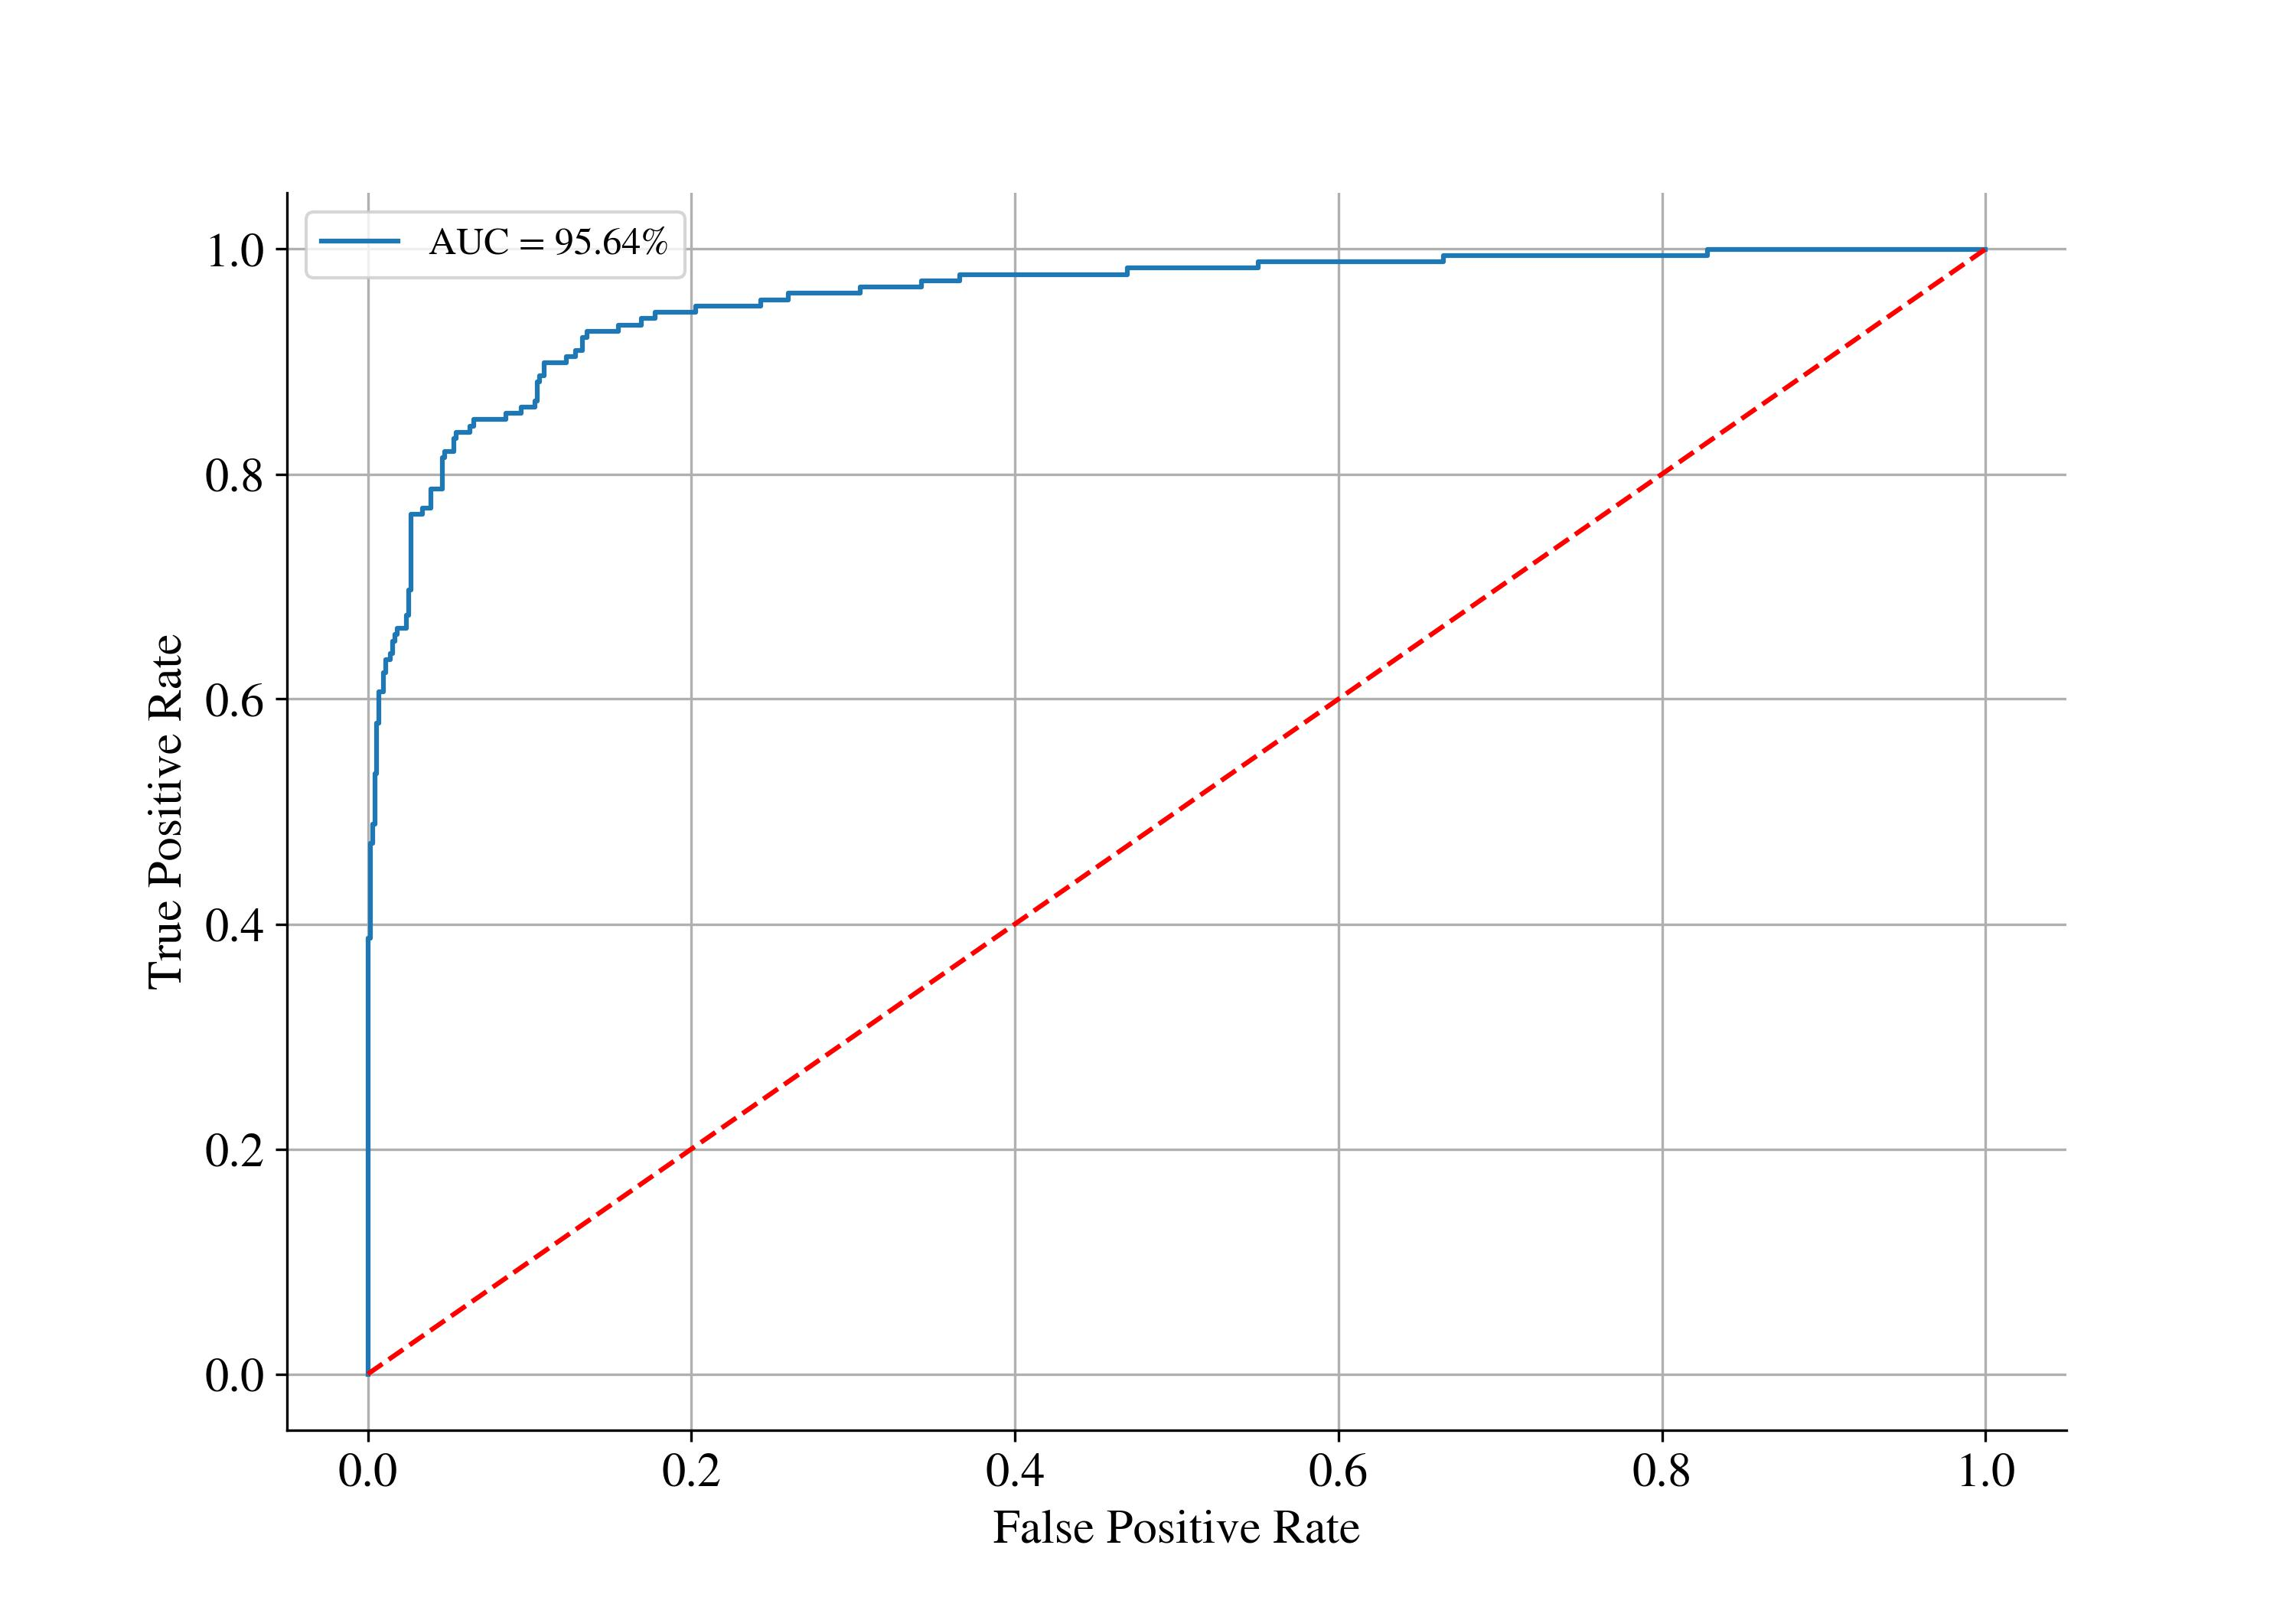
\includegraphics[width=140mm]{Figures/ROC_curve_FINAL.jpg}
\centering{\begin{source}Author's results in Python\end{source}}\vspace{-1em}
\end{figure}

\subsection{Model Explainability}
To gain insights into the impact of the features used in the final model, we can inspect the feature imporances of the final model, which is a part of family of tree ensemble algorithms.
As the name indicates, it is the score value representing the importance of the features, i.e., the higher score, the more important the feature is. Basically, it is the measure of how much a feature contributes to the overall performance of the model.
Overall, the feature importance plot provides valuable insights into the factors that are most important in predicting loan defaults. It can be used to identify which features are contributing the most to the model's accuracy and to guide future feature selection efforts.
According to Bonaccorso \citep{bonaccorso2020mastering}, feature importance is the measure proportional to the impurity reduction that a particular feature allows us to achieve, and is defined as:
\begin{equation}\label{eq}
    \text{FI}\left(\bar{x}^{\left(i\right)}\right) = \frac{1}{N} \displaystyle\sum_{k=1}^{N} \displaystyle\sum_{j=1}^{L} \frac{n(j)}{M} \delta I_{j}^{i}
\end{equation}
where $ \text{FI}\left(\bar{x}^{\left(i\right)}\right)$ referes to the feature importance of the feature $i$, $n(j)$ is the number of samples reaching the node $j$, $\delta I_{j}^{i}$ represents the impurity reduction at node $j$ after the splitting using the feature $j$, $M$ is total number of samples in the data set used to built the model, and $N$ refers to the number of tree estimators used within an ensemble model.

The following \autoref{fig:fi} depicts the feature importances of all the selected features on which the model was trained.
The two most important features used in the final model are \texttt{DEBTINC} and \texttt{DELINQ}, which are crucial delinquency indicators in determining whether a borrower would be able to repay their loan. These two features have a significant impact on the model's ability to accurately predict loan defaults, with high feature importance scores. This is also in line with the findings from the exploratory analysis, WoE distribution or feature selection.
\begin{figure}[H]
\centering
\caption{Feature Importance}\vspace{0.5em}
\label{fig:fi}\
\includegraphics[width=140mm]{Figures/Feature_Importances.jpg}
\centering{\begin{source}Author's results in Python\end{source}}\vspace{-1em}
\end{figure}

Thus, understanding the impact of individual features on model performance can be useful in identifying areas for improvement, as well as in identifying the most significant factors that drive loan defaults.
By focusing on these important features, lenders and policymakers can better understand and address the underlying factors that contribute to default risk, ultimately leading to better lending decisions and improved outcomes for borrowers and lenders alike.

\textbf{ADD BRIEF THEORY ABOUT THE SHAP VALUES}

To gain further insights into the impact of the features on the final model's predictions, the SHapley Additive exPlanations (henceforth SHAP) summary plot is displayed in \autoref{fig:shap}.
The SHAP summary plot provides a clear visualization of the contribution each feature makes to a prediction and is used for a black box model explainability.
Each dot in the plot represents a feature and its corresponding SHAP value.
The color of the dot represents the feature's value, with red indicating high values and blue indicating low values.
The position of the dot on the x-axis represents the impact of the feature on the prediction, with features on the right-hand side contributing more positively to the prediction, and features on the left-hand side contributing more negatively.

Since our data points are encoded in WoE values, the higher (the more positive) value, the larger distribution of non-defaulters compared to defaulters, and vice versa, the lower (the more negative) value, the larger distribution of defaulters compared to non-defaulters.
For the most important features, we can observe that the blue values (negative WoE values) and red values (positive WoE values) are quite separable.
Negative WoE values are positively contributing to the predictions, and the positive WoE values are negatively contributing to the predictions. This means that the more negative the WoE value, the more likely the borrower is to default, and vice versa.

Overall, the SHAP summary plot provides a valuable tool for interpreting and understanding the complex decision-making process of the final model.
The plot enables us to examine the impact of individual features on the model's output and helps us to identify which features are most influential in the model's decision-making process.
By understanding the relative importance of each feature, we can gain deeper insights into the creditworthiness assessment process and make more informed decisions in the lending industry.

\begin{figure}[H]
\centering
\caption{SHAP Summary Plot}\vspace{0.5em}
\label{fig:shap}\
\includegraphics[width=140mm]{Figures/SHAP_summary_plot.jpg}
\centering{\begin{source}Author's results in Python\end{source}}\vspace{-1em}
\end{figure}


\newpage
\section{Machine Learning Deployment}
This section describes the process of taking a trained machine learning model and making it available for use in the real world. It involves taking the model from a development environment and integrating it into a production environment where it can be used to make predictions or decisions based on new data. In this thesis, the machine learning model is deployed as web application using Flask and HTML.
\subsection{Final Model Recalibration}
Before deploying the model in a production setting, a meticulous process is undertaken to ensure optimal performance.
This involves conducting a final recalibration of the model using the entire data set, comprising the training, validation, and test sets.
The purpose of this recalibration is to fine-tune the model parameters, thereby maximizing its ability to generalize and yield accurate predictions.

The test set, which has been employed previously during the model evaluation phase, is incorporated into the recalibration process without any risk of data leakage.
By including the test set, the sample size for training is expanded, thereby increasing the model's capacity to generalize effectively.

Upon completion of the recalibration, the final classification threshold for deployment is determined to be \textbf{0.3358}.
This value is derived from a comprehensive analysis of the training, validation, and test sets, which ensures that the model's generalization capabilities are further enhanced for optimal performance in real-world applications.

\subsection{Flask and HTML Web Application}

In this case, the machine learning model is deployed into a web application using Flask and HTML. The application is temporarily deployed on the Cloud server on the \textbf{PythonAnywhere} platform and is accessible here: \url{http://ml-credit-risk-app-petrngn.pythonanywhere.com/}.
However, the application will be shut down after the thesis defense and will not be available online anymore due to the budget reasons.
Nevertheless, the code for the application is available in the GitHub repository, and the application can be run locally using any Python compiler.

Furthermore, prior to deployment, we need to prepare several Python inputs for the web application, including:
\begin{itemize}\setlength\itemsep{0em}
\item \textbf{Model} - the final model recalibrated on the training, validation and test set.
\item \textbf{Threshold} - the final classification threshold recalibrated on the training, validation and test set.
\item \textbf{Features} - the final features used in the final model.
\item \textbf{Data Frame} - the input tabular object used in the web application to store the loan applicant's inputs.
\item \textbf{Optimal Binning Transformator} - fitted \lstinline{BinningProcess} object for binning and WoE-encoding of the loan applicant's inputs.
\item \textbf{WoE Bins} - a set of bins and WoE values used for mapping the WoE values to missing values.
\item \textbf{LIME explainer} - fitted \lstinline{LimeTabularExplainer} object for local explainability of model's prediction.
\end{itemize}

Such inputs required for the machine learning application are exported in the \lstinline{.pkl} format using the \lstinline{dill} module. This format allows for efficient and easy-to-use serialization and deserialization of the inputs. The pickled file is then loaded directly into the Flask application.

For the back-end of the web application, Flask is used to deploy the machine learning model. The Flask application is written in the \lstinline{app.py} file, which is stored in the \lstinline{flask_app} directory. The front-end of the web application is coded in HTML, with CSS and JavaScript elements used to enhance the user interface.

The web application first renders a HTML page, as shown in \autoref{fig:flaskform}.
This page contains a loan application form, in which the user or the loan applicant fills in the respective field values that correspond to the features on which the machine learning model was trained.
The form is designed to capture the necessary information required for the model to make a prediction about the loan applicant's application.
Note that not all fields in the loan application form need to be filled out. This is because the missing values in certain features may indicate a higher risk of default. Conversely, one may choose to impose a restriction on the form, requiring all fields to be filled out. However, this could result in a lower number of received applications from delinquent clients, as they may not have all the necessary information to complete the form.
\begin{figure}[H]
\centering
\caption{Flask Web Application Form}\vspace{0.5em}
\label{fig:flaskform}\
\includegraphics[width=140mm]{Figures/flask_app_form.jpg}

\centering{\begin{source}Author's results in Python\end{source}}\vspace{-1em}
\end{figure}
\clearpage

Once, the loan application form is submitted, the web application uses the pickled input to transform the data from the loan application form and use it in the recalibrated model in order to get the result, whether the given loan applicant would repay his loan based on predetermined threshold. The result is then displayed in the web application, as shown in \autoref{fig:flaskres}.
Particularly, the web application returns whether the loan application would be denied or approved based on the model's output and also the probability score of default.

\begin{figure}[H]
\centering
\caption{Flask Web Application - Prediction Result}\vspace{0.5em}
\label{fig:flaskres}\
\includegraphics[width=130mm]{Figures/flask_app_result.jpg}

\centering{\begin{source}Author's results in Python\end{source}}\vspace{-1em}
\end{figure}

Besides the prediction results, it also displays the Local Interpretable Model-Agnostic Explanations (henceforth LIME) of the black--box model with respect to the inputs submitted within the form.
LIME focuses on the local explainability of the black box model around the black--box prediction as it generates a new data set consisting of perturbed samples around the given prediction and then trains a surrogate linear model on the new data set.
Such local interpretable, surrogate model should be a good approximation of the black box model in the vicinity of the given prediction, i.e., the local interpretable model is then used to explain the prediction of the black box model \citep{ribeiro2016should}.

The LIME explanation of input instances $x$ is given as follows:
\begin{equation}\label{eq}
\xi(x) = \arg\min_{g \in G} L(f, g, \pi_x) + \Omega(g)
\end{equation}

where $f$ is the original black--box model, $g$ is the surrogate model, $L$ is the loss functions measuring how far is the explanation $\xi(x)$ far from the prediction produced by black--box model $f$, and $\Omega(g)$ is the complexity of the surrogate model $g$.


The explanation is given in terms of the feature importance, which is represented by the magnitude of the feature's coefficient in the local interpretable model. The higher the magnitude of the coefficient, the more important the feature is in the prediction of the black box model.
Therefore, as it is shown in \autoref{fig:flaskres}, the red bars indicate positive contribution to the probability of default whereas green bars indicate negative contribution to the probability of default. In other words, The features with red bars indicate that the client would not probably repay his loan and vice versa.
The contributions' magnitudes are in line with the findings from feature imporance or SHAP values which is focused on the global explainability of the black--box model (not local explainability), that features such as debt--to--income ratio (\texttt{DEBTINC}) or number of deliquent credit lines (\texttt{DELINQ}) have the largest impact of the probability default.
Particularly, a high value of debt--to--income ratio causes higher probability default, whereas no delinquent credit lines leads to the lower probability default.

\chapter{Summary of Results}
\label{chap:five}
In this chapter, we evaluate the hypotheses presented in \autoref{sec:hypotest}, as outlined in \autoref{sec:hypo}.
These evaluations are based on the results obtained from the implementation of machine learning techniques described in \autoref{chap:four}. 
Furthermore, we compare our results with those of previous studies on HMEQ--based studies \citep{serkan2021bagging,zurada2014classification} in \autoref{sec:comparisonfinal}.
Additionally, we provide a summary of the key findings derived from the machine learning implementation from \autoref{chap:four} in  \autoref{sec:keyfindings}. 
Moreover, we delve into the author's contributions to the field of credit risk modelling and machine learning in \autoref{sec:contributions}.
Lastly, we address the key recommendations to improve this thesis and its machine learning implementation or for future research in \autoref{sec:recommendations}.

\section{Hypotheses' Testing}
\label{sec:hypotest}
\noindent \textbf{Result \#1:} \textit{The recalibration of the model \underline{DOES} enhace model performance on HMEQ data set.}

We fail to reject the \textbf{Hypothesis \#1} because we observe improvements across all the metrics within evaluation on test set when the final model was re-trained on the joined training and validation set instead solely on the training set.
In particular, all the score metrics and loss metrics have increased and decreased, respectively, as can be seen in \autoref{tab:recab}. Hereby, we can confirm that the recalibration of the model truly boost the model predictive power on HMEQ data set.

\vspace{0.3cm}

\noindent \textbf{Result \#2:} \textit{Neural Network and KNN model \underline{DO NOT} outperform all the models on HMEQ data set.}

We reject the \textbf{Hypothesis \#2} as the final model, which is the best performing, is the Gradient Boosting model as described in \autoref{tab:finalmodelinfo}.
KNN was also outperformed by the Random Forest and in case of Neural Network, it was outperformed by SVM as well, as can be seen in \autoref{fig:avgrankdist}.
If we aggregate the model selection results by looking the highest rank per each model, we can observe that the best KNN model had the 12th highest rank, while Neural Network (MLP) exhibited unsatisfactory performance with the 26th highest rank as can be seen in \autoref{tab:maxranks}.
Therefore, our results are not in with line with the outcomes of respective studies \citep{serkan2021bagging,zurada2014classification} which reported that Neural Network and KNN model outperformed all the models on HMEQ data set, respectively.

\begin{table}[H]
    \small
    \setlength{\tabcolsep}{8pt}
    \renewcommand{\arraystretch}{1.3}
    \centering
        \caption[Max--Aggregated Ranks of Models]{Max--Aggregated Ranks of Models}\label{tab:maxranks}
        \begin{tabular}{r r}
    \toprule
    \textbf{Model} & \textbf{Rank}\\
    \midrule
    \hline
    GB & 1 \\ 
    RF & 6 \\ 
    KNN & 12 \\ 
    SVM & 17 \\ 
    MLP & 26 \\ 
    DT & 35 \\ 
    LR & 39 \\
    GNB & 52 \\
    \hline
    \bottomrule
    \end{tabular}
    \vspace{0.35em}

        \centering{\begin{source}Author's results in Python\end{source}}\vspace{-1em}
\end{table}

\vspace{0.3cm}

\noindent \textbf{Result \#3:} \textit{Black--box models \underline{DO} perform better than the white--box models on HMEQ data set.}

We fail to reject the \textbf{Hypothesis \#3} as the black--box models truly outperformed the white--box models as can be seen in \autoref{fig:avgrankdistbbwb}, which depicts the distribution of ranks for both black--box and white--box models.
Most of the white--box models were ranked in the bottom half within the model selection, whereas the 10 best performing models consisted out of black--box models only, namely Gradient Boosting and Random Forest.
Even though that some black--box models' performances were weak and other white--box models exhibited relatively high ranks, we can still conclude that the black--box models outperformed the white--box models on average as the median of the black--box models' ranks is lower than the white--box models' median.
\vspace{0.3cm}

\noindent \textbf{Result \#4:} \textit{The longer execution time of a model \underline{DOES NOT} indicate better performance on HMEQ data set.}

We reject the \textbf{Hypothesis \#4} as according to \autoref{fig:timedist}, even though the Neural Network (MLP) model had the longest execution time on average, it underperformed several models such as Gradient Boosting, Random Forest, KNN and SVM which took significantly less time to execute. The same can be observed from \autoref{fig:scattertime}, where Neural Network performed poorly regardless the length of the execution time.
\vspace{0.3cm}

\noindent \textbf{Result \#5:} \textit{Debt and delinquency features \underline{ARE} the main default drivers on HMEQ data set.}

We fail to reject the \textbf{Hypothesis \#5} according to \autoref{fig:fi} which depicts the feature importance of the final model (Gradient Boosting). As can be seen, the most important features are debt--to--income ratio \texttt{DEBTINC} and number of delinquent credit lines \texttt{DELINQ}.
Based on the SHAP values depicted in \autoref{fig:shap}, we can observe that the negative values of \texttt{DEBTINC} and \texttt{DELINQ} positively contribute to the model's predictions of the target variable, whereas the positive values negatively contribute to the model's predictions.
In other words, the higher value of such features, the higher probability of default and vice versa.
Since the features' values are encoded as WoE, the negative WoE values indicates larger distribution of defaulters compared to non--defaulters in given bins.
Based on the WoE bins distribution in \autoref{fig:woedistdebtinc} and \autoref{fig:woedistdelinq}, respectively, we can observe negative WoE values for bins where the debt--to--income ratio is extremely high or is missing and regarding to the number of delinquent credit lines, we can observe a negative WoE value for bin corresponding to the relatively high number of delinquent credit lines.
Therefore, if the loan applicant has either high or missing debt--to--income ratio and/or relatively high number of delinquent credit lines, he would be likely to default.

\newpage
\section{Comparison with other HMEQ Studies}
\label{sec:comparisonfinal}
Within the literature review in \autoref{chap:three}, we disscused the studies of Aras \citep{serkan2021bagging} and Zurada \citep{zurada2014classification} which analyzed the HMEQ data set, i.e., the same data set as in this thesis.
In this section, we contrast their results with those of this thesis. Particularly, we compare the models' rankings from \autoref{tab:serkanresultsranks} and \autoref{tab:zuradaresultsranks}, respectively, with the thesis' author's rankings derived from \autoref{tab:maxranks}, which is summarized in the following \autoref{tab:comparisonfinal}.
Upon examination, it is apparent that none of the studies considered the Gradient Boosting model, which happens to be the best-performing model in this thesis.

With respect to the study of Aras \citep{serkan2021bagging}, when excluding our Gradient Boosting model, we can agree that Random Forest and KNN are the top-performing models. However, there is a discrepancy in the order of their performance. Aras found that KNN outperformed Random Forest, whereas in this thesis, Random Forest outperformed KNN.
Furthermore, it is worth noting that the worst-performing models, namely Decision Tree, Logistic Regression, and Gaussian Naive Bayes, align with both this thesis and Aras' study. Specifically, Aras identified Logistic Regression as the worst-performing model, while in this thesis, Gaussian Naive Bayes exhibited the poorest performance.

Regarding the Zurada's study \citep{zurada2014classification}, we again concur that Logistic Regression is one of the worst performing models.
However, there are significant disparities in the rankings of other models compared to the results obtained in this thesis.
It is evident from the findings that MLP was identified as the best performing model in Zurada's study, whereas in this thesis, MLP was ranked as the 5th best performing model, placing it in the second half of the ranked models.
In contrast, while KNN was ranked as the 3rd best performing model in this thesis, it received the position of the 2nd worst performing model according to Zurada.
Conversely, Zurada ranked Decision Tree as the best second performing model, while in this thesis, it was positioned as the 6th best performing model.
However, both Zurada's and Aras' studies, consistent with this thesis, ranked the SVM model in the middle range, aligning with our findings.
\begin{table}[H]
    \small
    \setlength{\tabcolsep}{8pt}
    \renewcommand{\arraystretch}{1.3}
    \centering
        \caption[Ranking Results Comparison based on HMEQ Data Set]{Ranking Results Comparison based on HMEQ Data Set}\label{tab:comparisonfinal}
        \begin{tabular}{r r r r}
    \toprule
    \textbf{Model} & \textbf{This Thesis} & \textbf{\citep{serkan2021bagging}} & \textbf{\citep{zurada2014classification}}\\
    \midrule
    \hline
    GB & 1 & - & - \\ 
    RF & 2 & 2 & - \\ 
    KNN & 3 & 1 & 4 \\ 
    SVM & 4 & 3 & 3 \\ 
    MLP & 5 & - & 1 \\ 
    DT & 6 & 4 & 2 \\ 
    LR & 7 & 6 & 5 \\
    GNB & 8 & 5 & - \\
    \hline
    \bottomrule
    \end{tabular}
    \vspace{0.35em}

        \centering{\begin{source}Author's results in Python, Rankings of \citep{serkan2021bagging}, \citep{zurada2014classification}\end{source}}\vspace{-1em}
\end{table}

It is important to note that the author of the thesis, Aras, and Zurada employed distinct data preprocessing techniques and different data splits, leading to variations in the training, tuning, and evaluation samples, resulting in disparate outcomes.
While Zurada and Aras utilized Grid Search with cross-validation for hyperparameter tuning, the author of the thesis employed Bayesian Optimization with stratified cross-validation. Besides, each author used different hyperparameters' spaces.

Additionally, each author utilized different evaluation metrics. Aras utilized Accuracy, Recall, Precision, F1, and Matthews Correlation Coefficient, while Zurada employed Accuracy, Recall, and AUC.
In contrast, the author of the thesis employed a broader range of metrics, including Accuracy, Recall, Precision, F1, Matthews Correlation Coefficient, AUC, Kolmogorov-Smirnov Distance, Somers' D, Brier Score Loss, and Log Loss.
Moreover, it is worth mentioning that the authors may have used different software tools. The thesis' author utilized Python, while Zurada employed Weka, and the software used by Aras is unknown.
These various factors contribute to the discrepancies in the obtained results among the studies and the thesis. Therefore, it is advisable to refrain from making direct comparisons due to the incomparability of the results.
\vspace{0.3cm}

\newpage
\section{Key Findings}
\label{sec:keyfindings}
The key findings of this thesis are summarized in the following list. We exclude such findings which are derived from the hypotheses' testing in \autoref{sec:hypotest}, namely that the most important features for predicting default are the number of delinquent credit lines \texttt{DELINQ} and the debt--to--income ratio \texttt{DEBTINC}, and that the Gradient Boosting model outperforms all other models in terms of the majority of evaluation metrics etc.

\begin{itemize}\setlength\itemsep{0em}
    \item ADASYN oversampling generates more default--case instances which are managers according to \texttt{JOB} feature as described in depicted in \autoref{tab:adasynimpact} and \autoref{fig:adasynimpact}.
    This is attributed to ADASYN nature as it generates more synthetic instances for such default--case instances which are hard-to--learn, therefore default clients who are managers are hard--to--learn according to ADASYN and its underlying KNN algorithm as described in \autoref{subsec:data-split-ADASYN}. By generating more synthetic learn for instances which are hard--to--learn, ADASYN oversampling is expected to improve the model's performance.
    \item We can also observe the impact of missing values within default prediction, particularly in case of debt--to--income ratio \texttt{DEBTINC}. As can be seen in \autoref{fig:woedistdebtinc}, the WoE corresponding the bin capturing missing values has a negative value of (approx. -2), which indicates a larger distribution of defaulters compared to non--defaulters.
    Referring to the WoE values, the SHAP summary plot (\autoref{fig:shap}) depicts the global model explainability and the contribution of each feature to the predictions. As can be seen in case of \texttt{DEBTINC}, the blue values (i.e., negative WoE values) contributes positively to the default, hence when the debt--to--income ratio is missing, the model is more likely to predict default for such instance.
    \item Another finding regards the features \texttt{DEBTINC} and \texttt{DELINQ}. The higher debt--to--income ratio and/or the higher number of delinquent credit lines, the higher the probability of default. This is evident from the WoE values in \autoref{fig:woedistdebtinc} and \autoref{fig:woedistdelinq}, respectively, and the SHAP summary plot in \autoref{fig:shap}.
    \item Most of the models are conservative as most of their optimal thresholds obtained using Youden index are below the standard classification threshold of 0.5 as depicted in \autoref{fig:thresdistclean}.
    \item Ensemble models, such as Gradient Boosting and Random Forest, perform better than SVM or Neural Network (MLP), while the transparent models such as Decision Tree, Logistic Regression, and Gaussian Naive Bayes perform the worst. This is depicted in \autoref{fig:avgrankdist}.
    \item Black--box models which are complex tend to select more features than transparent white box--models within feature selection (\autoref{fig:fsrec}).
\end{itemize}
\section{Contributions}
\label{sec:contributions}
The primary contribution of the thesis author involves the implementation of a customized machine learning framework on a credit risk dataset consisting of performing and non-performing US home equity loans, as described in \autoref{fig:mlframe} from high--level point of view. This framework encompasses several key steps.

Firstly, the author conducts data exploration (\autoref{sec:dataexploration}), including distribution and association analysis. To address the imbalanced distribution of defaults, an advanced approach utilizing ADASYN oversampling is employed (\autoref{subsec:data-split-ADASYN}).
Additionally, a preprocessing step utilizing Optimal Binning is implemented to discretize feature values into bins optimized with respect to the default status, while also capturing the impact of extreme and missing values by converting them into Weight-of-Evidence values (\autoref{subsec:prep-optbinning}).

The author then utilizes custom wrapped algorithms for both feature selectionand model selection.
These algorithms incorporate Bayesian Optimization for hyperparameter tuning based on the chosen classification models (\autoref{subsec:hyperoptbayes}).
Within the feature selection, algorithm, each model is tuned and used within Forward Sequential Feature Selection to determine the subset of optimal features  (\autoref{subsec:feature-selection}).
Within the model selection algorithm, each model is tuned and trained on subsets of selected features, determining an optimal threshold for classification using the Youden index, and subsequently evaluated on a validation set using a variety of metrics (\autoref{subsec:modelselection}).
The models are ranked based on these metrics, considering explicit weights defined by the author.
The best performing model is selected for final evaluation on the test set and for deployment.

To enhance the model's performance and generalization ability, the author performs recalibration of the model and threshold prior to evaluation, by joining the training and validation sets into one set used for model recalibration (\autoref{subsec:modelrecal}).
The evaluation process encompasses various approaches, including the assessment of the model's performance using a confusion matrix, evaluation metric scores and losses, and ROC curve analysis (\autoref{subsec:modelperformance}).
The impact of recalibration on the evaluation is also examined.
Additionally, the author assesses the explainability of the black-box model by analyzing feature importances and SHAP values (\autoref{subsec:explainability}).

Another significant contribution involves deploying the model as a web application using Flask and HTML (\autoref{sec:deployment}).
The deployed application is recalibrated alongside its threshold on the joined training, validation and test sets to enhace model's ability to generalize.
Such application is temporarily hosted and deployed on PythonAnywhere cloud platform and made publicly accessible.
Users are required to complete a loan application form, with the fields corresponding to the features on which the model was trained.
After submission, the application provides a result and default prediction, accompanied by explainability insights using LIME, which highlights the contribution of each feature to the prediction (\autoref{subsec:flaskapp}).


\section{Recommendations}
\label{sec:recommendations}
Despite the complexity of the custom machine learning solution applied in this thesis, and the hundreds of hours invested by the author, it still has its limitations and drawbacks. We aim to address these issues in this section and provide suggestions for future studies.
\begin{enumerate}\setlength\itemsep{0em}
    \item \textbf{Use more relevant and actual data} - Given the nature of the data set analyzed in this thesis, it might not be the most relevant for the current market situation. Thus, using an up-to-date data would either lead to a more realistic generalization \citep {kumar2021blockchain} or an improvement in model's performance \citep{karatas2020increasing}.
    \item \textbf{Use bigger data} - Since the real bank data sets often contain hunders of thousands or even millions of instances, and the number of features can be in hundreds or even higher, it would be beneficial to use bigger data sets to train the models on. Therefore, having bigger sample size for the training, we can enhace model's performance \citep{ng2020influence}, as the model would be able to learn more complex patterns in the data. 
    \item \textbf{Use behavioral scoring data} - The data set used in this thesis is based on the application data only, however, the behavioral scoring data is often used in the real--world applications as well. Therefore, it would be also beneficial to use behavioral scoring data which would dynamically capture the client's information about his behavior and it would help the bank to make more informed decision about how to deal with the existing clients \citep{li2012overview}.
    \item \textbf{Use macroeconomic data} - Using macroeconomic data such as GDP, unemployment rate, inflation rate, interest rate etc. would allow to create macroeceonomic forecasts, i.e., to take into account possible changes in the macroeconomic changes by incorporating forward--looking information \citep{jakubik2007macroeconomic}.
    Thanks to that, one would be able to achieve more more reliable estimates by would dynamically capturing the current economic situation.
    \item \textbf{Use TensorFlow/Keras or PyTorch for NN development} - In this thesis, we used Neural Network (Multi--Layer Percepton) from \lstinline{Scikit-learn} module. Howeover, in ML engineering or deep learning, the Neural Networks are mostly developed using TensorFlow/Keras or Keras modules which are more efficient and provide more flexibility \citep{gevorkyan2019review}.
    \item \textbf{Django for ML deployment} - In this thesis, a Flask framework was used for ML deployment as a web application. Although Flask is a great tool for ML deployment when it comes to the small projects or micro-framework solutions, it is not suitable for production environment.
    Therefore, we recommend to use Django framework for ML deployment, which is a full--stack Python--based web application framework and is more suitable for production environment and creating larger more complex database--backed websites and applications \citep{khatri2023}.
    \item \textbf{ML implementation in other credit risk modelling components} - Besides applying ML prediction models in credit risk for default prediction (i.e., PD), it would be also beneficial to apply ML models in other credit risk modelling components such as LGD and EAD, ECL \citep{munkhdalai2019empirical, grzybowska2020application} or even for macroeceonomic forecasting \citep{hall2018machine}.
    \item \textbf{Hyperparameter Optimization with Optuna} - In this thesis, we used Bayesian Optimization from \lstinline{Scikit-optimize} module for hyperparameter optimization. However, there are more efficient framwork, namely Optuna module, which is deemed as the next--generation hyperparameter optimization software which allows to construct the hyperparameter search space dynamically, efficient implementation of searching and pruning strategies and it also provides
    a versatile architecture which can be deployed in scalable distributed computing or light--weight experiments conducted through interactive interface \citep{akiba2019optuna}.
    \item \textbf{H2O ML library} - H2O is an automated machine learning library which is more efficient than \lstinline{Scikit-learn} and provides more flexibility in terms of faster scoring capabilities or producing high quality models suitable for deployment in enterprise envinronment \citep{ledell2020h2o}. 
    According to H2O's documentation, it provides wrapper functions which perform a large number of modelling-related tasks that would typically require many lines of code and it can be also used for automating the machine learning workflow including automatic training and tuning of many models \citep{H2Oai2023}.
\end{enumerate}
\chapter{Conclusion}
\label{conclusion}

The main contribution of this thesis is to develop a custom machine learning implementation framework using Python which is further applied to the application scoring data set of US home equity loans (HMEQ).
In this thesis, we use 8 machine learning classification models - Logistic Regression, Decision Tree, Gaussian Naive Bayes, K--Nearest Neighbors, Random Forest, Gradient Boosting, Support Vector Machine, and Neural Network (Multi--Layer Perceptron). As evaluiation metrics, we use F1 score, Precision, Recall, Accuracy, Matthews Correlation Coefficient, AUC, Kolmogorov--Smirnov Distance, Somers' D, Brier Score Loss and Log Loss.

Within this thesis, we have covered theoretical background of credit risk as well as particular machine learning algorithms and the evaluation of classification models, including more advanced machine learning techniques such as ADASYN oversmapling, Optimal Binning, Bayesian Optimization or Forward Sequential Feature Selection, as all described in \autoref{chap:two}.
In \autoref{chap:three} we have proposed five hypothesess, including the literature review with the main focus on HMEQ--based studies of Aras \citep{serkan2021bagging} and Zurada \citep{zurada2014classification}.

The \autoref{chap:four} pertains to the very extensive empirical analysis, i.e., machine learning implementation on HMEQ data set.  This includes the high--level overview of the custom machine learning framework, repository and envinronment structure in Python (\autoref{sec:repo}), data exploration, data preprocessing, hyperparameter tuning, feature selection, model selection, model recalibration, model evaluation and final machine learning deployment.
Within data exploration (\autoref{sec:dataexploration}), we delve into the description of the data set, disribution analysis and association analysis.

This chapter further employs an data preprocessing step (\autoref{sec:dataprep}), including the data split into training set (for hyperparameter tuning, feature selection and model training), validation set (for model selection), and test set (for model evaluation).
Such data is split into ratio 70:15:15 with stratification and further, ADASYN oversampling is performed in order to balance the default distribution (\autoref{subsec:data-split-ADASYN}).
The next step of data preprocessing involves Optimal Binning (\autoref{subsec:prep-optbinning}), which is utilized using \lstinline{optbinning} module in Python developed by Navas--Palencia \citep{navas2020optimal}. This module is employed in order to discretize the numeric features into interval bins and categorical features into subgroups of categories, both are optimally binned with respect to the default, and further transforms these bins using Weight--of--Evidence.


\autoref{chap:four} also contains modelling part (\autoref{sec:modelling}), which includes Bayesian Optimization, feature selection and model selection.
Bayesian Optimization is used for hyperparameter tuning, particularly we use \lstinline{scikit-optimize} module which employes Bayesian Optimization with 50 iterations, stratified 10--fold cross validation, while maximizing F1 score. For each model, we further define hyperparameters' spaces over which the model is tuned (\autoref{subsec:hyperoptbayes}).
The feature selection (\autoref{subsec:feature-selection}) is performed using custom algorithm developed by the author, which iterates over the models. Each model is tuned with Bayesian Optimization on training set and is further used as an input estimator within Forward Sequential Feature Selection on training set, which returns subset of optimal features for given model. Since we have eight models, we obtain eight subset of features.
Within the model selection \autoref{subsec:modelselection}, each model is tuned on each subset of selected features on training set, and then is evaluated on the validation set by computing several evaluation metrics.
Instead of using standard classification threshold of 0.5, we compute an optimal threshold using Youden index. Since we have 8 models and 8 subsets of features, we obtain 64 models in total.
All the models are ranked on each metric, based on which we calculate a rank score as a weighted average of the individual ranks, where the weights are set explicitly by the author. Based on the rank score, we determine the final rank. The model with the highest rank (i.e., rank of 1) is then selected as the final model for both evaluation and deployment.
The final model is \textbf{Gradient Boosting} which was trained on the features selected by \textbf{Multi--Layer Perceptron}.

Such final model is then recalibrated on the joined training and validation set and also, the optimal threshold is recalculated using Youden index, as described in \autoref{subsec:modelrecal}.
afterwards, the final recalibrated model is evaluated on test set (\autoref{sec:modeleval}), where we assess the model performance, inspect impact of the recalibration on the model's predictive power and also we delve into black--box model explainability using feature importances and SHAP summary plot. It is evident that debt--to--income ratio and number of delinquent credit lines are the main default drivers.

In the last part of machine learning implementation, the final model is deployed into a production enviroment (\autoref{sec:deployment}).
Prior the deployment, the final model and its optimal threshold are recalibrated on the whole data set (training, validation and test set) in order to maximize the predictive power of the model.
Particularly, such model is deployed as a web application built in Flask (back--end) and HTML with CSS and JavaScript elements (front-end). The web application itself is temporarily deployed on PythonAnywhere cloud platform which is accessible via the folllowing link: \url{http://ml-credit-risk-app-petrngn.pythonanywhere.com/}.
This application requires to fill in the loan application form where its fields correspond to the features on which the final model was trained (\autoref{fig:flaskform}). After a submission of the form, the application processes the inputs, bins them and transforms them into WoE values and afterwards, it predicts the result, whether the loan is rejected or approved based on the optimal threshold, and the probability of default. The result is then displayed on the web page (\autoref{fig:flaskres}).
The application also displays LIME which depicts the local Explainability of the model around the given prediction, i.e., it shows the contribution of each feature to the prediction.

In the last \autoref{chap:five}, we summarize the results of this thesis. Particularly, we assess hypotheses' testing (\autoref{sec:hypotest}) which is depicted in  \autoref{tab:hypoconclusion}.

This chapter also includes the discussion of the model rankings results with the results of the studies of Aras \citep{serkan2021bagging} and Zurada \citep{zurada2014classification} as discussed in \autoref{sec:comparisonfinal}.
While the results of Aras' study are in line with the results of this thesis, i.e., Random Forest and K-Nearest Neighbors perform well whereas Decision Tree, Logistic Regression and Gaussian Naive Bayes perform poorly,
the results of Zurada's study are not in line with the results of this thesis, as its best models are Multi--Layer Perceptron and Decision Tree, which are outperformed by Gradient Boosting, Random Forest, K-Nearest Neighbors and Support Vector Machine.
Further, Zurada ranks K-Nearest Neighbors as one the worst performing models (after Logistic Regression), whereas K-Nearest Neighbors performs well in this thesis and outperforms Support Vector Machine, Multi--Layer Perceptron, Decision Tree, Logistic Regression and Gaussian Naive Bayes.
Since either thesis' author, Zurada and Aras used different data preprocessing steps, hyperparameter tuning approach and spaces, evaluation metrics and software tools, we should refrain from making direct comparisons due to the incomparability of the results, given the factors mentioned above.

Regarding the key findings of this thesis, particularly of the machine learning implementation \autoref{sec:keyfindings}, besides the findings observed within hypotheses' testing and studies' comparisons, we further observe that ADASYN oversampling generates more default--case instances which are managers
which is attributed to the nature of ADASYN oversampling,
which generates more synthetic default--case samples for such default cases which are hard--to--learn by ADASYN,
thus defaulted managers are hard--to--learn by ADASYN (\autoref{subsec:data-split-ADASYN}).
By generating more syntehtic instances which are hard--to--learn, it is expected that the model's performance will be enhanced.
Another finding regards the impact of the missing value of debt--to--income ratio within default prediction, in particular, if the debt--to--income ratio is missing, it increases the probability of default (\autoref{fig:shap}), since bin capturing missing values has negative WoE coefficient (\autoref{fig:woedist}).
Following this observation, also higher of debt-to--income ratio and/or number of delinquent credit lines increase the probability of default as can be seen in SHAP summary plot (\autoref{fig:shap}) and WoE distribution (\autoref{fig:woedist}).
Further, most of the models are conservative since their optimal thresholds are lower than the standard classification threshold 0.5, i.e., they are more likely to reject the loan application than to approve it, as depicted in \autoref{fig:thresdistclean}.
Moreover, ensemble models, such as Gradient Boosting and Random Forest, outperform Support Vector Machine and Multi--Layer Perceptron, whereas the less complex, white--box models, such as Decision Tree, Logistic Regression and Gaussian Naive Bayes have very poor performance, as shown in \autoref{fig:avgrankdist}.
Last but not least, Black--box models which are complex require more features than transparent white box--models to perform well within feature selection (\autoref{fig:fsrec}).

In the final part, we discuss the contribution of this thesis which is further elaborated in detail in \autoref{sec:contributions}, and the recommendations for future research \autoref{sec:keyfindings}, given the limitation of the analyzed data set which might not be representative for the current situation in the financial industry.
We recommend to use more relevant actual data to capture current market situation; use bigger data to increase the training sample size; use macroeconomic data to dynamically capture the current economic state;
use TensorFlow/Keras or PyTorch for development of Neural Network which is more versatile than Scikit-learn; use Django for machine learning deployment which is more suitable for full--stack projects than Flask;
implement machine learning in other components of credit risk modelling, such as EAD, LGD, recovery rates or ECL itself; use Optuna module for hyperparameter tuning which is the state--of--the--art hyperparameter optimization framework; use H2O module for automated machine learning.
\clearpage
%-----<<< -------- >>>-----

%-----<<< REFERENCES >>>-----
\fancyhead[LO]{\sffamily Bibliography}					%headers in sans serif and not in uppercase
\bibliographystyle{Styles/Stylebib}							%style of literature, you can use e.g. newapa	instead of Styles/Stylebib
\bibliography{Styles/Bibliography}							%bibliography database
\addcontentsline{toc}{chapter}{Bibliography} 		%Add bibliography to the table of contents
\clearpage
%-----<<< ---------- >>>-----

%-----<<< APPENDIXES >>>-----
\backmatter																			%uppercase roman pagination for back matter; appendices start
\autohdr																				%automatic headers     				
\chapter{Additional Figures and Tables}
\label{chap:app1}

\begin{table}[H]
    \small
    \setlength{\tabcolsep}{8pt}
    \renewcommand{\arraystretch}{1.3}
    \centering
        \caption[Normality Test - Shapiro--Wilk]{Normality Test - Shapiro--Wilk}\label{tab:normalitytest}
        \begin{tabular}{rrrr}
    \toprule
    \textbf{Feature} & \textbf{Shapiro-Wilk} & \textbf{Significance} & \textbf{Result}\\
    \midrule
    \hline
    LOAN & 0.8519 & *** & Not normally distributed \\ 
    MORTDUE & 0.8802 & *** & Not normally distributed \\ 
    VALUE & 0.8100 & *** & Not normally distributed \\ 
    YOJ & 0.9078 & *** & Not normally distributed \\ 
    DEROG & 0.3360 & *** & Not normally distributed \\ 
    DELINQ & 0.4578 & *** & Not normally distributed \\ 
    CLAGE & 0.9346 & *** & Not normally distributed \\ 
    NINQ & 0.6909 & *** & Not normally distributed \\ 
    CLNO & 0.9665 & *** & Not normally distributed \\ 
    DEBTINC & 0.8272 & *** & Not normally distributed \\
    \hline
    \bottomrule
    \end{tabular}
    \vspace{0.35em}

        \centering{\begin{source}Author's results in Python\end{source}}\vspace{-1em}
\end{table}


\begin{figure}[H]
    \centering
    \caption{ADASYN Impact of Numeric Features' Distribution}\vspace{0.5em}
    \label{fig:adasynimpactnum}
    \includegraphics[width=140mm]{Figures/Numeric_Features_Distribution_OS_Violinplots.jpg}
    
    \centering{\begin{source}Author's results in Python\end{source}}\vspace{-1em}
\end{figure}


\begin{figure}[H]
    \centering
    \caption{WoE Bins Distribution}\vspace{0.5em}
    \label{fig:woedist}
    \includegraphics[width=100mm]{Figures/WoE_Distribution.jpg}
    
    \centering{\begin{source}Author's results in Python\end{source}}\vspace{-1em}
\end{figure}

\section{Model Selection Results}

\begin{figure}[H]
    \centering
    \caption{Precision Distribution}\vspace{0.5em}
    \label{fig:precdist}
    \includegraphics[width=140mm]{Figures/PRECISION_Distribution.jpg}
    
    \centering{\begin{source}Author's results in Python\end{source}}\vspace{-1em}
\end{figure}

\begin{figure}[H]
    \centering
    \caption{Precision Distribution - \textit{without outlier}}\vspace{0.5em}
    \label{fig:precdistwoout}
    \includegraphics[width=140mm]{Figures/PRECISION_WO_OUTLIERS_Distribution.jpg}
    
    \centering{\begin{source}Author's results in Python\end{source}}\vspace{-1em}
\end{figure}

\begin{figure}[H]
    \centering
    \caption{Precision Distribution (Black--box/White--box dimension)}\vspace{0.5em}
    \label{fig:precdistbbwb}
    \includegraphics[width=140mm]{Figures/PRECISION_Distribution_BB_WB.jpg}
    
    \centering{\begin{source}Author's results in Python\end{source}}\vspace{-1em}
\end{figure}

\begin{figure}[H]
    \centering
    \caption{Precision Distribution (Black--box/White--box dimension) - \textit{without outlier}}\vspace{0.5em}
    \label{fig:precdistwooutbbwb}
    \includegraphics[width=140mm]{Figures/PRECISION_WO_OUTLIERS_Distribution_BB_WB.jpg}
    
    \centering{\begin{source}Author's results in Python\end{source}}\vspace{-1em}
\end{figure}



\begin{figure}[H]
    \centering
    \caption{Recall Distribution}\vspace{0.5em}
    \label{fig:reccdist}
    \includegraphics[width=140mm]{Figures/RECALL_Distribution.jpg}
    
    \centering{\begin{source}Author's results in Python\end{source}}\vspace{-1em}
\end{figure}

\begin{figure}[H]
    \centering
    \caption{Recall Distribution - \textit{without outlier}}\vspace{0.5em}
    \label{fig:recdistwoout}
    \includegraphics[width=140mm]{Figures/RECALL_WO_OUTLIERS_Distribution.jpg}
    
    \centering{\begin{source}Author's results in Python\end{source}}\vspace{-1em}
\end{figure}

\begin{figure}[H]
    \centering
    \caption{Recall Distribution (Black--box/White--box dimension)}\vspace{0.5em}
    \label{fig:recdistbbwb}
    \includegraphics[width=140mm]{Figures/RECALL_Distribution_BB_WB.jpg}
    
    \centering{\begin{source}Author's results in Python\end{source}}\vspace{-1em}
\end{figure}

\begin{figure}[H]
    \centering
    \caption{Recall Distribution (Black--box/White--box dimension) - \textit{without outlier}}\vspace{0.5em}
    \label{fig:recdistwooutbbwb}
    \includegraphics[width=140mm]{Figures/RECALL_WO_OUTLIERS_Distribution_BB_WB.jpg}
    
    \centering{\begin{source}Author's results in Python\end{source}}\vspace{-1em}
\end{figure}

\begin{figure}[H]
    \centering
    \caption{Accuracy Distribution}\vspace{0.5em}
    \label{fig:accdist}
    \includegraphics[width=140mm]{Figures/ACCURACY_Distribution.jpg}
    
    \centering{\begin{source}Author's results in Python\end{source}}\vspace{-1em}
\end{figure}

\begin{figure}[H]
    \centering
    \caption{Accuracy Distribution (Black--box/White--box dimension)}\vspace{0.5em}
    \label{fig:accdistbbwb}
    \includegraphics[width=140mm]{Figures/ACCURACY_Distribution_BB_WB.jpg}
    
    \centering{\begin{source}Author's results in Python\end{source}}\vspace{-1em}
\end{figure}

\begin{figure}[H]
    \centering
    \caption{AUC Distribution}\vspace{0.5em}
    \label{fig:aucdist}
    \includegraphics[width=140mm]{Figures/AUC_Distribution.jpg}
    
    \centering{\begin{source}Author's results in Python\end{source}}\vspace{-1em}
\end{figure}

\begin{figure}[H]
    \centering
    \caption{AUC Distribution (Black--box/White--box dimension)}\vspace{0.5em}
    \label{fig:aucdistbbwb}
    \includegraphics[width=140mm]{Figures/AUC_Distribution_BB_WB.jpg}
    
    \centering{\begin{source}Author's results in Python\end{source}}\vspace{-1em}
\end{figure}

\begin{figure}[H]
    \centering
    \caption{Matthews Correlation Coefficient Distribution}\vspace{0.5em}
    \label{fig:mccdist}
    \includegraphics[width=140mm]{Figures/MCC_Distribution.jpg}
    
    \centering{\begin{source}Author's results in Python\end{source}}\vspace{-1em}
\end{figure}

\begin{figure}[H]
    \centering
    \caption{Matthews Correlation Coefficient Distribution - \textit{without outlier}}\vspace{0.5em}
    \label{fig:mccdistwoout}
    \includegraphics[width=140mm]{Figures/MCC_WO_OUTLIERS_Distribution.jpg}
    
    \centering{\begin{source}Author's results in Python\end{source}}\vspace{-1em}
\end{figure}

\begin{figure}[H]
    \centering
    \caption{Matthews Correlation Coefficient Distribution (Black--box/White--box dimension)}\vspace{0.5em}
    \label{fig:mccdistbbwb}
    \includegraphics[width=140mm]{Figures/MCC_Distribution_BB_WB.jpg}
    
    \centering{\begin{source}Author's results in Python\end{source}}\vspace{-1em}
\end{figure}

\begin{figure}[H]
    \centering
    \caption{Matthews Correlation Coefficient Distribution (Black--box/White--box dimension) - \textit{without outlier}}\vspace{0.5em}
    \label{fig:mccdistwooutbbwb}
    \includegraphics[width=140mm]{Figures/MCC_WO_OUTLIERS_Distribution_BB_WB.jpg}
    
    \centering{\begin{source}Author's results in Python\end{source}}\vspace{-1em}
\end{figure}

\begin{figure}[H]
    \centering
    \caption{Brier Score Loss Distribution}\vspace{0.5em}
    \label{fig:bsldist}
    \includegraphics[width=140mm]{Figures/BRIER SCORE LOSS_Distribution.jpg}
    
    \centering{\begin{source}Author's results in Python\end{source}}\vspace{-1em}
\end{figure}

\begin{figure}[H]
    \centering
    \caption{Brier Score Loss Distribution (Black--box/White--box dimension)}\vspace{0.5em}
    \label{fig:bsldistbbwb}
    \includegraphics[width=140mm]{Figures/BRIER SCORE LOSS_Distribution_BB_WB.jpg}
    
    \centering{\begin{source}Author's results in Python\end{source}}\vspace{-1em}
\end{figure}

\begin{figure}[H]
    \centering
    \caption{Kolmogorov--Smirnov Distance Distribution}\vspace{0.5em}
    \label{fig:ksdist}
    \includegraphics[width=140mm]{Figures/KS_Distribution.jpg}
    
    \centering{\begin{source}Author's results in Python\end{source}}\vspace{-1em}
\end{figure}

\begin{figure}[H]
    \centering
    \caption{Kolmogorov--Smirnov Distance Distribution (Black--box/White--box dimension)}\vspace{0.5em}
    \label{fig:ksdistbbwb}
    \includegraphics[width=140mm]{Figures/KS_Distribution_BB_WB.jpg}
    
    \centering{\begin{source}Author's results in Python\end{source}}\vspace{-1em}
\end{figure}

\begin{figure}[H]
    \centering
    \caption{Log Loss Distribution}\vspace{0.5em}
    \label{fig:loglossdist}
    \includegraphics[width=140mm]{Figures/LOG LOSS_Distribution.jpg}
    
    \centering{\begin{source}Author's results in Python\end{source}}\vspace{-1em}
\end{figure}

\begin{figure}[H]
    \centering
    \caption{Log Loss Distribution (Black--box/White--box dimension)}\vspace{0.5em}
    \label{fig:loglossdistbbwb}
    \includegraphics[width=140mm]{Figures/LOG LOSS_Distribution_BB_WB.jpg}
    
    \centering{\begin{source}Author's results in Python\end{source}}\vspace{-1em}
\end{figure}

\begin{figure}[H]
    \centering
    \caption{Somers' D Distribution}\vspace{0.5em}
    \label{fig:sddist}
    \includegraphics[width=140mm]{Figures/SOMERS D_Distribution.jpg}
    
    \centering{\begin{source}Author's results in Python\end{source}}\vspace{-1em}
\end{figure}

\begin{figure}[H]
    \centering
    \caption{Somers' D Distribution (Black--box/White--box dimension)}\vspace{0.5em}
    \label{fig:sddistbbwb}
    \includegraphics[width=140mm]{Figures/SOMERS D_Distribution_BB_WB.jpg}
    
    \centering{\begin{source}Author's results in Python\end{source}}\vspace{-1em}
\end{figure}           			%input file
\KOMAoptions{paper=landscape,DIV=last}
\newgeometry{hmargin=2.5cm,bottom=25mm,height=150mm, includehead}
\fancyheadoffset{0pt}
\chapter{Source Codes}


\section{Python Notebook Code}
\begin{lstlisting}[basicstyle=\footnotesize\ttfamily]
import warnings

warnings.filterwarnings("ignore")

import os
import numpy as np
import pandas as pd
import matplotlib
import matplotlib.pyplot as plt
from matplotlib import ticker
import seaborn as sns
import time
import math
import missingno
from itertools import combinations

from scipy.stats import chi2_contingency, ks_2samp, pointbiserialr, somersd
from imblearn.over_sampling import ADASYN

from optbinning import BinningProcess

from sklearn.model_selection import train_test_split, StratifiedKFold
from sklearn.feature_selection import SequentialFeatureSelector
from sklearn.metrics import (
	accuracy_score,
	recall_score,
	precision_score,
	f1_score,
	matthews_corrcoef,
	brier_score_loss,
	confusion_matrix,
	roc_curve,
	roc_auc_score,
	log_loss,
)


from sklearn.linear_model import LogisticRegression
from sklearn.tree import DecisionTreeClassifier
from sklearn.naive_bayes import GaussianNB
from sklearn.ensemble import RandomForestClassifier, GradientBoostingClassifier
from sklearn.neighbors import KNeighborsClassifier
from sklearn.svm import SVC
from sklearn.neural_network import MLPClassifier

from skopt import BayesSearchCV
from skopt.space import Real, Categorical, Integer
import shap

import lime
import dill

data = pd.read_csv("./data/raw_data.csv")
\end{lstlisting}
\subsection{Data Exploration}
\begin{lstlisting}[basicstyle=\footnotesize\ttfamily]
data.info()

no_duplicates = data.duplicated(subset = [col for col in data.columns if col != 'BAD']).sum()
print(f"Duplicates check: {no_duplicates} duplicated rows.")


def categorical_numeric_vars(df: pd.DataFrame, target:str = "BAD") -> tuple[list, list]:
    
    cat_vars = [col for col in df.columns if df[col].dtypes == "O" and col != target]
    num_vars = [col for col in df.columns if col not in cat_vars + [target]]

    print(f"Categorical features: {', '.join(cat_vars)}")
    print(f"Numeric features: {', '.join(num_vars)}")

    return (cat_vars, num_vars)

cat_vars, num_vars = categorical_numeric_vars(data)


def default_distribution_plot(df, target="BAD", export=True):
    
    matplotlib.rcParams["mathtext.fontset"] = "stix"
    matplotlib.rcParams["font.family"] = "STIXGeneral"
    
    # Replacing the Booleans with non-default/default strings for visualization
    df_plot = df[[target]].copy().replace({0: "Non-default", 1: "Default"})

    # Figure's initialization
    fig, ax = plt.subplots(figsize=(8, 6))
    
    # Default distribution
    sns.countplot(data=df_plot, x=target, palette="BuPu",
                  order=list(df_plot[target].unique())[::-1], ax=ax)
    
    # Increase the fontsize for xlabel and ylabel
    ax.set_ylabel(ax.yaxis.label.get_text(), fontsize=17)
    ax.set_xlabel(ax.xaxis.label.get_text(), fontsize=17)

    # Increase the fontsize for xticks and yticks
    plt.xticks(fontsize=17)
    plt.yticks(fontsize=17)

    # Removing upper and right axes spines
    ax.spines["top"].set_visible(False)
    ax.spines["right"].set_visible(False)

    plt.tight_layout()
    
    # Exporting plot
    if export:
        os.makedirs("./plots/", exist_ok=True)
        plt.savefig(f"./plots/Default_Distribution.jpg", dpi=300)

    plt.show()

default_distribution_plot(data)


def numeric_distribution_plot(df: pd.DataFrame, num_vars: list,
                                 plot_type: str, target: str = "BAD", 
                                 export: bool = True):

    def custom_int_formatter(x, pos):
        return f"{x:.0f}"

    #Possible plot types
    plot_types = {"boxplot": sns.boxplot,
                  "violinplot": sns.violinplot,
                  "histogram": sns.histplot}

    #Plot type parameter check
    if plot_type not in plot_types.keys():
		plot_types = ','.join([key for key in plot_types.keys()])
        raise ValueError(f"Invalid plot type. Please, select one of these available plot types: {plot_types}")

        
    matplotlib.rcParams["mathtext.fontset"] = "stix"
    matplotlib.rcParams["font.family"] = "STIXGeneral"
    
    #Plot either boxplots or violinplots
    if plot_type in ["boxplot", "violinplot"]:
        
        #replace 0/1's with (Non)-default texts for visualization's sake.
        df_plot = df.copy()
        df_plot[target] = df_plot[target].replace({0: "Non-default", 1: "Default"})

        #Figure's and axes' initialization
        fig, axs = plt.subplots(nrows = 5, ncols = 2, figsize = (12, 20))

        for ax, var in zip(axs.ravel(), num_vars):
            
            #Boxplot/violinplot
            plot_types[plot_type](data = df_plot, x = target, y = var, ax = ax,
                                  palette = "BuPu", order = ["Non-default", "Default"])

            ax.set_title(f"Distribution of {var}", size = 19, fontweight = "bold")
            ax.tick_params(axis = "both", which = "major", labelsize = 18)
            ax.set(xlabel = None)
            ax.set(ylabel = None)
            ax.spines["top"].set_visible(False)
            ax.spines["right"].set_visible(False)
            ax.yaxis.set_major_formatter(matplotlib.ticker.FuncFormatter(custom_int_formatter))
        
        plt.tight_layout()

        #Exporting the plots
        if export:
            os.makedirs("./plots/", exist_ok = True)
            plt.savefig(f"./plots/Numeric_Features_Distribution_{plot_type.capitalize()}s.jpg", dpi = 300)
        plt.show()


    #Plot histograms
    elif plot_type == "histogram":
        def integer_formatter(x, pos):
            return f"{int(x)}"

        #Figure's and axes' initialization
        fig, axs = plt.subplots(nrows = len(num_vars), ncols = 2, figsize = (12, 25))

        #Column index
        col_ind = 0
        # Axis index
        # (if the value is even, the plot will be located on the left side, otherwise on the right side)
        axis_count = 0

        for ax in axs.ravel():

            #Accessing the feature name.
            var = num_vars[col_ind]
            #Subsetting the data based on the feature.
            var_series = df[var]

            # Calculating the bin size for given feature ensuring that both conditional plots
            # (left and right) will have the same number of bins.
            # Using rule of thumb (Scott, 1979)
            # https://stackoverflow.com/questions/33458566/how-to-choose-bins-in-matplotlib-histogram
       
            R = var_series.max() - var_series.min() #Range of the feature's values
            n = len(var_series) #Number of feature's values
            sigma = var_series.std() #Standard deviation of the feature's values
        
            #Number of bins
            no_bins = int(R*(n**(1/3))/(3.49*sigma))

            # The left side (even axis_count) depicts the features' distribution
            # conditional on the non-default cases.
            if axis_count % 2 == 0:
                #Subsetting the data for non-default cases only.
                df_subset= df.query(f"{target} == 0")
                #Number of missing values within given feature
                no_missings = df_subset[var].isna().sum()
                # Percentage of missing values within subset of given feature
                # (i.e., percentage of missing values of given feature within the non-default cases)
                pct_missings = no_missings/df_subset.shape[0] * 100

                # Histogram with kernel density function
                # binrange to ensure that both left and right plot will have the same data range.
                plot_types[plot_type](data = df_subset, x = var, ax = ax, bins = no_bins,
                                binrange = ((var_series.min(), var_series.max())),
                                kde = True, color = "lightblue")
 
                ax.set_title(f"Distribution of {var} (Non-default cases)", size = 17, fontweight = "bold")
                ax.tick_params(axis = "both", which = "major", labelsize = 15, rotation = 30)
                ax.set(xlabel = None)
                ax.set_ylabel(ax.get_ylabel(), fontsize=15)
                ax.xaxis.set_major_formatter(ticker.FuncFormatter(integer_formatter))
                ax.spines["top"].set_visible(False)
                ax.spines["right"].set_visible(False)

                #Inserting a text box with an information about the missing values.
                ax.text(0.7, 0.9, f"Number of NA's: {no_missings} ({pct_missings:.1f}%)",
                       horizontalalignment = "center", verticalalignment = "center",
                       fontsize = 14,
                       transform = ax.transAxes, bbox = dict(facecolor = "pink", alpha = 0.3))

            # The right side (odd axis_count) depicts the features' distribution
            # conditional on the default cases.
            else:
                #Subsetting the data for default cases only.
                df_subset = df.query(f"{target} == 1")
                #Number of missing values within given feature
                no_missings = df_subset[var].isna().sum()
                # Percentage of missing values within subset of given feature
                # (i.e., percentage of missing values of given feature within the default cases)
                pct_missings = no_missings/df_subset.shape[0] * 100

                # Histogram with kernel density function
                # binrange to ensure that both left and right plot will have the same data range.
                sns.histplot(data = df_subset, x = var, ax = ax, bins = no_bins,
                                binrange = ((var_series.min(), var_series.max())),
                                kde = True, color = "mediumpurple")
                
                ax.set_title(f"Distribution of {var} (Default cases)", size = 17, fontweight = "bold")
                ax.tick_params(axis = "both", which = "major", labelsize = 15, rotation = 30)
                ax.set(xlabel = None)
                ax.set_ylabel(ax.get_ylabel(), fontsize=15)
                ax.xaxis.set_major_formatter(ticker.FuncFormatter(integer_formatter))
                ax.spines["top"].set_visible(False)
                ax.spines["right"].set_visible(False)

                #Inserting a text box with an information about the missing values.
                ax.text(0.7, 0.9, f"Number of NA's: {no_missings} ({pct_missings:.1f}%)",
                        horizontalalignment = "center", verticalalignment = "center",
                        fontsize = 14,
                        transform = ax.transAxes, bbox = dict(facecolor = "pink", alpha = 0.3))
                
                #Proceeding with the next feature
                col_ind += 1

            #Switching to the left/right side of the figure
            axis_count +=1
        
        plt.tight_layout()
        
        #Exporting the plots
        if export:
            os.makedirs("./plots/", exist_ok = True)
            plt.savefig(f"./plots/Numeric_Features_Distribution_{plot_type.capitalize()}s.jpg", dpi = 300)
    
        plt.show()


numeric_distribution_plot(data, num_vars, plot_type = "boxplot")
numeric_distribution_plot(data, num_vars, plot_type = "violinplot")
numeric_distribution_plot(data, num_vars, plot_type = "histogram")


def normality_test(data: pd.DataFrame, num_vars: list) -> pd.DataFrame:

    from scipy.stats import shapiro

    output_df = pd.DataFrame(columns = ["Feature", "Shapiro-Wilk", "Significance", "Result"])
    
    for i, col in enumerate(num_vars):
        temp_df = data.copy()
        temp_df = temp_df[temp_df[col].notna()].copy()

        output_df.loc[i, "Feature"] = col

        shapiro_stat, shapiro_p = shapiro(temp_df[col])
        shapiro_significance_stars = "***" if shapiro_p < 0.01 else "**" if shapiro_p < 0.05 \ 
		                            else "*" if shapiro_p < 0.1 else ""
        shapiro_significance_result = "Normally distributed" if shapiro_p > 0.05 \
                                       else "Not normally distributed"

        output_df.loc[i, "Shapiro-Wilk"] = round(shapiro_stat,4)
        output_df.loc[i, "Significance"] = shapiro_significance_stars
        output_df.loc[i, "Result"] = shapiro_significance_result
        
    return output_df


normality_test(data, num_vars)


def num_na_table(df: pd.DataFrame, num_vars: list, target: str = "BAD") -> pd.DataFrame:
    output_df = pd.DataFrame(index = num_vars,
                      columns = ["# of NA's (Y=0)", "# of NA's (Y=1)",  "% of NA's (Y=0)", "% of NA's (Y=1)"])
    for num in num_vars:
        output_df.loc[num, "# of NA's (Y=0)"] = df.query(f"{target} == 0")[num].isna().sum()
        output_df.loc[num, "# of NA's (Y=1)"] = df.query(f"{target} == 1")[num].isna().sum()

        pct_nd = df.query(f"{target} == 0")[num].isna().sum()/df.query(f"{target} == 0").shape[0] * 100
        pct_d = df.query(f"{target} == 1")[num].isna().sum()/df.query(f"{target} == 1").shape[0] * 100
        output_df.loc[num, "% of NA's (Y=0)"] = pct_nd
        output_df.loc[num, "% of NA's (Y=1)"] = pct_d

    return output_df

num_na_table(data, num_vars)


def categorical_distribution_plot(df: pd.DataFrame, cat_vars: list,
                                  target: str = "BAD", export: bool = True):
    
    #Figure's and axes' initialization
    fig, axs = plt.subplots(nrows = len(cat_vars),ncols = 2, figsize = (11, 10))

    #Column index
    col_ind = 0
    # Axis index
    # (if the value is even, the plot will be located on the left side, otherwise on the right side)
    axis_count = 0
    
    matplotlib.rcParams["mathtext.fontset"] = "stix"
    matplotlib.rcParams["font.family"] = "STIXGeneral"
    
    for ax in axs.ravel():

        #Accessing the feature name
        var = cat_vars[col_ind]
        # Subsetting the data based on the feature with subsequent replacing missing values
        # with N/A's strings (for visualization's sake).
        var_target_df = df[[var, target]].copy().fillna("N/A")
        
        #If the feature has some missing values, put the N/A category at the end of the plot.
        if var_target_df.query(f"{var} == 'N/A'").shape[0] != 0:
            categories = [cat for cat in var_target_df[var].unique() if cat != "N/A"] + ["N/A"]
        else:
            categories = var_target_df[var].unique()

        # The left side (even axis_count) depicts the features' distribution
        # conditional on the non-default cases.
        if axis_count % 2 == 0:

            sns.countplot(data = var_target_df.query(f"{target} == 0"), x = var,
                          ax = ax, order = categories, color = "lightblue")

            ax.set_title(f"Distribution of {var} (Non-default cases)", size = 19, fontweight = "bold")
            ax.tick_params(axis = "both", which = "major", labelsize = 18)
            ax.tick_params(axis = "x", rotation = 30, which = "major", labelsize = 18)
            ax.set(xlabel = None)
            ax.set_ylabel(ax.get_ylabel(), fontsize=15)
            ax.spines["top"].set_visible(False)
            ax.spines["right"].set_visible(False)
                        
        
        # The right side (odd axis_count) depicts the features' distribution
        # conditional on the default cases.
        else:
            
            sns.countplot(data = var_target_df.query(f"{target} == 1"), x = var,
                          ax = ax, order = categories, color = "mediumpurple")

            ax.set_title(f"Distribution of {var} (Default cases)", size = 19, fontweight = "bold")
            ax.tick_params(axis = "both", which = "major", labelsize = 18)
            ax.tick_params(axis = "x", rotation = 30, which = "major", labelsize = 18)
            ax.set_ylabel(ax.get_ylabel(), fontsize=15)
            ax.set(xlabel = None)
            ax.spines["top"].set_visible(False)
            ax.spines["right"].set_visible(False)

            #Proceeding with the next feature
            col_ind += 1

        #Switching to the left/right side of the figure
        axis_count += 1

    plt.tight_layout()

    #Exporting the plots
    if export:
        os.makedirs("./plots/", exist_ok = True)
        plt.savefig(f"./plots/Categorical_Features_Distribution.jpg", dpi = 300)
        
    plt.show()


categorical_distribution_plot(data, cat_vars)


def cat_na_table(df: pd.DataFrame, cat_var: str, target: str = "BAD") -> pd.DataFrame:
    temp_df = df.copy()
    temp_df[cat_var] = temp_df[cat_var].fillna("N/A") 
    output_df = pd.DataFrame(index = list(temp_df[cat_var].unique()),
                             columns = ["# (Y=0)", "# (Y=1)",  "% (Y=0)", "% (Y=1)"])

    for cat in output_df.index:
        output_df.loc[cat, "# (Y=1)"] = temp_df.query(f"{target} == 1 and {cat_var} == '{cat}'").shape[0]
        output_df.loc[cat, "# (Y=0)"] = temp_df.query(f"{target} == 0 and {cat_var} == '{cat}'").shape[0]
        pct_d = round(output_df.loc[cat, "# (Y=1)"]/temp_df.query(f"{target} == 1").shape[0], 4)* 100
        pct_nd = round(output_df.loc[cat, "# (Y=0)"]/temp_df.query(f"{target} == 0").shape[0] , 4)* 100
        output_df.loc[cat, "% (Y=1)"] = pct_d
        output_df.loc[cat, "% (Y=0)"] = pct_nd

    return output_df

cat_na_table(data, "JOB")
cat_na_table(data, "REASON")

def point_biserial_corr_table(data: pd.DataFrame, num_features, target = 'BAD') -> pd.DataFrame:
    
    output_df = pd.DataFrame(columns = ['Feature', 'Point-Biserial Correlation', 'Significance'])
    for i, col in enumerate(num_features):
        
        temp_df = data[data[col].notna()].copy()
        coef, p_value = pointbiserialr(temp_df[target], temp_df[col])
        output_df.loc[i, 'Feature'] = col
        output_df.loc[i, 'Point-Biserial Correlation'] = round(coef, 3)

        significance_stars =  '***' if p_value <= 0.01 else '**' if p_value <= 0.05 else \
		              '*' if p_value <= 0.1 else ' '
        output_df.loc[i, 'Significance'] = significance_stars

    return output_df
    

point_biserial_corr_table(data, num_vars)


def cramer_v_table(data: pd.DataFrame, cat_features, target = 'BAD') -> pd.DataFrame:
    
    output_df = pd.DataFrame(columns = ['Variable #1',  'Variable #2', "Cramer's V", 'Significance'])

    pairs = list(combinations(cat_features + [target], 2))

    pairs =  [sorted(pair) for pair in pairs]

    pairs = sorted(pairs)

    for i, pair in enumerate(pairs):
        temp_df = data.copy()
        temp_df = temp_df[temp_df[pair[0]].notna()]
        temp_df = temp_df[temp_df[pair[1]].notna()]

        cross_tab = pd.crosstab(temp_df[pair[0]], temp_df[pair[1]])
        chi2, p_value, *_ = chi2_contingency(cross_tab, correction = False)

        N = cross_tab.sum().sum()
        k = min(cross_tab.shape)
        cr_v = np.sqrt((chi2/N) / (k-1))

        significance_stars =  '***' if p_value <= 0.01 else '**' if p_value <= 0.05 else \
		               '*' if p_value <= 0.1 else ' '

        output_df.loc[i, 'Variable #1'] = pair[0]
        output_df.loc[i, 'Variable #2'] = pair[1]
        output_df.loc[i, "Cramer's V"] = round(cr_v, 3)

        significance_stars =  '***' if p_value <= 0.01 else '**' if p_value <= 0.05 else \
		              '*' if p_value <= 0.1 else ' '
        output_df.loc[i, 'Significance'] = significance_stars

    return output_df


cramer_v_table(data, cat_vars)


def phi_correlation(var1, var2) -> float:

    cross_tab = pd.crosstab(var1, var2)

    chi2, p_value, *_ = chi2_contingency(cross_tab)
    n = cross_tab.sum().sum() 

    phi = np.sqrt(chi2/n)
    
    return phi


def na_phi_corr_table(data: pd.DataFrame, target = 'BAD') -> pd.DataFrame:

    output_df = pd.DataFrame(columns = ['Feature', 'Phi Correlation', 'Significance'])

    for i, col in enumerate(data.drop(target, axis = 1).columns):
        na_indicator = [1 if pd.isnull(i) else 0 for i in data[col]]
        cross_tab = pd.crosstab(data[target], na_indicator)
        chi2, p_value, *_ = chi2_contingency(cross_tab)
        n = cross_tab.sum().sum() 

        phi = np.sqrt(chi2/n)
        significance_stars =  '***' if p_value <= 0.01 else '**' if p_value <= 0.05 else \
		              '*' if p_value <= 0.1 else ' '

        output_df.loc[i, 'Feature'] = col
        output_df.loc[i, 'Phi Correlation'] = round(phi, 3)
        output_df.loc[i, 'Significance'] = significance_stars

    return output_df

na_phi_corr_table(data)


def spearman_corr_matrix_plot(df: pd.DataFrame, num_var: list, export: bool = True):
    
    #Figure's initialization
    plt.figure(figsize = (16,13))
    matplotlib.rcParams['mathtext.fontset'] = 'stix'
    matplotlib.rcParams['font.family'] = 'STIXGeneral'
    #Corelation matrix heatmap
    heatmap = sns.heatmap(df[num_var].corr(method = "spearman"), vmin = -1, vmax = 1,
                        mask = np.triu(np.ones_like(df[num_var].corr())),
                        annot = True, cmap  = "coolwarm",  fmt = ".3f",
                        xticklabels = num_var, yticklabels = num_var,
                        annot_kws={"size": 19})

    plt.xticks(fontsize = 19)
    plt.yticks(fontsize = 19)

    cbar = heatmap.collections[0].colorbar
    cbar.ax.tick_params(labelsize=19)
    
    plt.tight_layout()

    #Exporting the plots
    if export:
        os.makedirs("./plots/", exist_ok = True)
        plt.savefig(f"./plots/Spearman_Correlation_Matrix_Numeric_Features.jpg", dpi = 300)
    
    plt.show()


spearman_corr_matrix_plot(data, num_vars)


def na_dendrogram(df:pd.DataFrame, export:bool = True, plot_suffix:str = ""):

    matplotlib.rcParams['mathtext.fontset'] = 'stix'
    matplotlib.rcParams['font.family'] = 'STIXGeneral'

    #True/False values indicating whether a column has some NA's.
    na_columns_indicators = df.describe(include = "all").T["count"] < df.shape[0]
    #Filtering the column names having NA's.
    na_columns = df.columns[na_columns_indicators]
    #Subsetting the data based on the NA's columns.
    final_df_dendogram = df[na_columns]

    #Plotting the dendrogram
    missingno.dendrogram(final_df_dendogram, orientation = "top", figsize = (10, 6), fontsize = 11)
    #plt.title("Dendrogram of variables having NA's", size = 13, fontweight = "bold")
    plt.yticks(fontsize=17)
    plt.xticks(rotation=45, fontsize=17)

    plt.tight_layout()

    #Exporting the plot
    if export:
        os.makedirs("./plots/", exist_ok = True)
        plt.savefig(f"./plots/NA_Dendrogram{plot_suffix}.jpg", dpi = 300)
    
    plt.show()

na_dendrogram(data)
na_dendrogram(data[data['BAD'] == 1], plot_suffix = "_defaults")
\end{lstlisting}

\subsection{Data Preprocessing}
\begin{lstlisting}[language=Python, basicstyle=\footnotesize\ttfamily]
	def data_split(
		df: pd.DataFrame,
		test_size: float,
		validation_size: float,
		seed: int,
		num_vars,
		cat_vars,
		oversampling: str = "None",
		target: str = "BAD",
	) -> tuple[pd.DataFrame, pd.Series, pd.DataFrame, pd.Series, pd.DataFrame, pd.Series]:
	
		# Separating the target variable (Y) and the features (X)
		Y = df[target]
		X = df.drop(target, axis=1)
	
		# Stratified split into training set, validation set and test set
		X_temp, X_test, y_temp, y_test = train_test_split(
			X, Y, stratify=Y, test_size=test_size, random_state=seed
		)
		X_train, X_valid, y_train, y_valid = train_test_split(
			X_temp, y_temp, stratify=y_temp, test_size=validation_size, random_state=seed
		)
	
		# ADASYN Oversampling
		if oversampling == "ADASYN":
	
			# ADASYN initialization
			adasyn = ADASYN(random_state=seed, n_jobs=-1)
	
			# Temporary imputing of missing values
			# (separately for categorical and numeric features)
			# ADASYN cannot work with NA's, thus we replace them with arbitrary values.
			X_train_imputed = pd.concat(
				(
					X_train[cat_vars].copy().fillna("NAN"),
					X_train[num_vars].copy().fillna(99999999999999),
				),
				axis=1,
			)[X_train.columns].copy()
	
			# Dummy encoding of categorical features
			# ADASYN cannot work with categorical features, thus we need to encode them.
			for cat in cat_vars:
				X_cat_dummies = pd.get_dummies(X_train_imputed[[cat]])
				X_train_imputed = X_train_imputed.drop(cat, axis=1)
				X_train_imputed = pd.concat((X_train_imputed, X_cat_dummies), axis=1)
	
			# Oversampling on the training set.
			X_train_final, y_train_final = adasyn.fit_resample(
				X_train_imputed, pd.DataFrame(y_train)
			)
	
			# Converting dummies back into the original categorical features.
			for cat in cat_vars:
				X_train_final[cat] = (
					X_train_final.loc[
						:, [col for col in X_train_final.columns if cat in col]
					]
					.idxmax(axis=1)
					.str.replace(f"{cat}_", "")
				)
				X_train_final = X_train_final.drop(
					[col for col in X_train_final.columns if f"{cat}_" in col], axis=1
				)
	
			# Replacing the NA's strings back to NA's with respect to the categorical features.
			X_train_final = X_train_final.replace({"NAN": np.nan})
	
			# Replacing back the missing values (99999999999999) with NA's in such case
			# whether the value is exceeding the maximum value of given numeric feature before imputing.
			for num in num_vars:
				max_value = X_train[num].max()
				X_train_final[num] = X_train_final[num].apply(
					lambda x: np.nan if x > max_value else x
				)
	
			y_train_final = y_train_final[target]
	
			X_train_final = X_train_final.reindex(columns=X_train.columns)
	
			return X_train_final, y_train_final, X_valid, y_valid, X_test, y_test
	
		# No oversampling
		else:
	
			return X_train, y_train, X_valid, y_valid, X_test, y_test


seed = 42
test_size = 0.15
validation_size = test_size/(1 - test_size)

(
    X_train,
    y_train,
    X_valid,
    y_valid,
    X_test,
    y_test,
) = data_split(data, test_size, validation_size, seed, num_vars, cat_vars, oversampling="ADASYN")

(
    X_train_orig,
    y_train_orig,
    X_valid_orig,
    y_valid_orig,
    X_test_orig,
    y_test_orig,
) = data_split(data, test_size, validation_size, seed, num_vars, cat_vars)


def print_data_info(**kwargs):
    
    for name, _set in kwargs.items():

        no_dashes = 50
        no_dashes_name_left = int((no_dashes - len(name) - 1)/2)*"-"
        no_dashes_name_right  = f"{(no_dashes - len(name) - len(no_dashes_name_left) - 2)*'-'}"

        data_info = f"{_set['features'].shape[0]} instances, {_set['features'].shape[1]} features"
        no_dashes_data_info_left = int((no_dashes - len(data_info) - 1)/2)*"-"
        no_dashes_data_info_right = f'{(no_dashes - len(data_info) - len(no_dashes_data_info_left) - 2)*"-"}'
        pct_d = np.sum(_set['target']) / _set['target'].shape[0]*100:
        pct_nd = np.sum(_set['target'] == 0)/ _set['target'].shape[0]*100
        target_info = f"Default: {pct_d:.2f}%  | Non-default: {pct_nd:.2f}%"
        no_dashes_target_info_left = int((no_dashes - len(target_info) - 1)/2)*"-"
        length_dashes_target_info_right = (no_dashes - len(target_info) - len(no_dashes_target_info_left) - 2)
        no_dashes_target_info_right = f'{length_dashes_target_info_right*"-"}'


        print(no_dashes*"-")
        print(f"{no_dashes_name_left} {name} {no_dashes_name_right}")
        print(f"{no_dashes_data_info_left} {data_info} {no_dashes_data_info_right}")
        print(f"{no_dashes_target_info_left} {target_info} {no_dashes_target_info_right}")
        print(no_dashes*"-", "\n")

print_data_info(Training = {'features': X_train, 'target': y_train},
                Validation = {'features': X_valid, 'target': y_valid},
                Test = {'features': X_test, 'target': y_test})


				def woe_binning(
					x_train_set: pd.DataFrame,
					y_train_labels: pd.Series,
					cat_vars: list,
					export: bool = True,
					**kwargs,
				) -> tuple[dict, pd.DataFrame]:
				
					binning_path = "./models/feature_preprocessing"
					final_objects_path = "./models/objects_FINAL"
				
					# Initializing the binning process object.
					bn = BinningProcess(
						variable_names=list(x_train_set.columns),
						categorical_variables=cat_vars
					)
				
					# Fitting the binning on training set.
					bn.fit(x_train_set, y_train_labels)
				
					# DataFrame including binned categories' information.
					bins_woe = pd.DataFrame()
				
					for i in x_train_set.columns:
				
						var = bn.get_binned_variable(i).binning_table.build()
						var = var[(~var["Bin"].isin(["Special", "Totals"]))]
						var["Variable"] = i
				
						bins_woe = pd.concat((bins_woe, var))
				
					bins_woe = bins_woe.loc[:, ~bins_woe.columns.isin(["JS"])]
				
					if export:
						for save_path in [binning_path, final_objects_path]:
							os.makedirs(save_path, exist_ok=True)
							bn.save(f"{save_path}/binning_woe_object.h5")
							bins_woe.to_csv(f"{save_path}/woe_bins.csv",
							   index = False)
				
					# Transforming both training set and test set
					# based on the fitted training binning.
					def woe_bin_transform(bn_fit, x_set):
						x_set_binned = bn_fit.transform(x_set, metric="woe")
						x_set_binned.index = x_set.index
				
						return x_set_binned
				
					X_binned_sets = {"X_train_binned": woe_bin_transform(bn, x_train_set)}
					x_set_copy = X_binned_sets["X_train_binned"].copy()
				
					for col in x_set_copy.columns:
						na_woe = (bins_woe
						         .query('Variable == @col and Bin == "Missing"')["WoE"]
							 .values[0]
							 )
						x_set_copy.loc[x_train_set[col].isna(), col] = na_woe
					X_binned_sets["X_train_binned"] = x_set_copy
				
					for name, x_set in kwargs.items():
						X_binned_sets[f"{name}_binned"] = woe_bin_transform(bn, x_set)
						x_set_copy = X_binned_sets[f"{name}_binned"].copy()
						for col in x_set_copy.columns:
							na_woe = (bins_woe
							         .query('Variable == @col and Bin == "Missing"')
								 ["WoE"]
					           		 .values[0])
							x_set_copy.loc[x_set[col].isna(), col] = na_woe
						X_binned_sets[f"{name}_binned"] = x_set_copy
				
					return (X_binned_sets, bins_woe, bn)

				
X_binned_sets, woe_bins, binning_transformator = woe_binning(X_train, y_train, cat_vars,
                                                             X_valid = X_valid, X_test = X_test)
X_train_binned, X_valid_binned, X_test_binned = (xset for i, xset in X_binned_sets.items())

X_binned_sets_orig, woe_bins_orig, binning_transformator_orig = woe_binning(X_train_orig, y_train_orig,
                                                                            export = False, cat_vars,
                                                                            X_valid = X_valid_orig,
                                                                            X_test = X_test_orig)
X_train_binned_orig, X_valid_binned_orig, X_test_binned_orig = (xset for i, xset in X_binned_sets_orig.items())


def prep_data_export(features: tuple, labels: tuple,
                     ind_sets: tuple = ("Training", "Validation", "Test"),
                     csv_name:str = '') -> pd.DataFrame:

    df_list = []
    
    #Join each pair of features and labels data, assign to it a set indicator,
        # append to the list and then,
        #  transform that list into a data frame (and export it).
    for feat, lab, ind in zip(features, labels, ind_sets):
        
        temp = pd.concat((lab, feat), axis = 1)
        temp["set"] = ind
        df_list.append(temp)
    
    dfs = [df for df in df_list]

    final_df = pd.concat(dfs, axis = 0).sort_index()

    if len(csv_name) != 0:
        os.makedirs("./data/", exist_ok = True)
        final_df.to_csv(f"./data/{csv_name}.csv", index = False)
    
    return final_df


interim = prep_data_export((X_train_binned, X_valid_binned, X_test_binned),
                            (y_train, y_valid, y_test),
                            ("Training", "Validation", "Test"),
                            csv_name = "interim_data")


def categorical_distribution_plot_OS(df_orig: pd.DataFrame, df_os, cat_vars: list,
                                  target: str = "BAD", class_val = 1, export: bool = False):
    
    #Figure's and axes' initialization
    fig, axs = plt.subplots(nrows = len(cat_vars),ncols = 2, figsize = (14, 10))

    #Column index
    col_ind = 0
    #Axis index (if the value is even, the plot will be located on the left side, otherwise on the right side)
    axis_count = 0
    
    matplotlib.rcParams['mathtext.fontset'] = 'stix'
    matplotlib.rcParams['font.family'] = 'STIXGeneral'

    class_title_name = 'Default' if class_val == 1 else 'Non-Default'
    
    for ax in axs.ravel():

        #Accessing the feature name
        var = cat_vars[col_ind]
        # Subsetting the data based on the feature with subsequent replacing missing values#
        # with N/A's strings (for visualization's sake).
        var_target_df_orig = df_orig[[var, target]].copy().fillna("N/A")
        var_target_df_os = df_os[[var, target]].copy().fillna("N/A")
        
        #If the feature has some missing values, put the N/A category at the end of the plot.
        if var_target_df_orig.query(f"{var} == 'N/A'").shape[0] != 0:
            categories_orig = [cat for cat in var_target_df_orig[var].unique() if cat != "N/A"] + ["N/A"]
        else:
            categories_orig = var_target_df_orig[var].unique()

        #If the feature has some missing values, put the N/A category at the end of the plot.
        if var_target_df_os.query(f"{var} == 'N/A'").shape[0] != 0:
            categories_os = [cat for cat in var_target_df_os[var].unique() if cat != "N/A"] + ["N/A"]
        else:
            categories_os = var_target_df_os[var].unique()

        # The left side (even axis_count) depicts the features' distribution
        # conditional on the non-default cases.
        if axis_count % 2 == 0:

            sns.countplot(data = var_target_df_orig.query(f"{target} == {class_val}"), x = var,
                          ax = ax, order = categories_orig, color = "lightblue")

            ax.set_title(f"Distribution of {var} ({class_title_name} cases)", size = 19, fontweight = "bold")
            ax.tick_params(axis = "both", which = "major", labelsize = 18)
            ax.tick_params(axis = "x", rotation = 30, which = "major", labelsize = 18)
            ax.set(xlabel = None)
            ax.set_ylabel(ax.get_ylabel(), fontsize=18)
            ax.spines["top"].set_visible(False)
            ax.spines["right"].set_visible(False)
                        
        
        #The right side (odd axis_count) depicts the features' distribution conditional on the default cases.
        else:
            
            sns.countplot(data = var_target_df_os.query(f"{target} == {class_val}"), x = var,
                          ax = ax, order = categories_os, color = "mediumpurple")

            ax.set_title(f"Distribution of {var} ({class_title_name} cases) - Oversampled",
                         size = 19, fontweight = "bold")
            ax.tick_params(axis = "both", which = "major", labelsize = 18)
            ax.tick_params(axis = "x", rotation = 30, which = "major", labelsize = 18)
            ax.set_ylabel(ax.get_ylabel(), fontsize=18)
            ax.set(xlabel = None)
            ax.spines["top"].set_visible(False)
            ax.spines["right"].set_visible(False)

            #Proceeding with the next feature
            col_ind += 1

        #Switching to the left/right side of the figure
        axis_count += 1

    plt.tight_layout()

    #Exporting the plots
    if export:
        os.makedirs("./plots/", exist_ok = True)
        plt.savefig(f"./plots/Categorical_Features_Distribution_OS_{class_title_name}.jpg", dpi = 300)
        
    plt.show()


categorical_distribution_plot_OS(pd.concat((X_train_orig, y_train_orig), axis = 1),
                                 pd.concat((X_train, y_train), axis = 1),
                                   cat_vars, class_val = 1, export = True)

df_temp = pd.DataFrame(columns = ['Feature', 'Category', '# (Y=1)', '# (Y=1) - Oversampled',
                                  '% (Y=1)','% (Y=1) - Oversampled'])
i = 0
orig_temp_df = pd.concat((X_train_orig, y_train_orig), axis = 1).copy()
temp_df = pd.concat((X_train, y_train), axis = 1).copy()
for cat_var in cat_vars:
    orig_temp_df[cat_var] = orig_temp_df[cat_var].fillna("N/A")
    temp_df[cat_var] = temp_df[cat_var].fillna("N/A")

    for category in orig_temp_df[cat_var].unique():
        df_temp.loc[i, 'Feature'] = cat_var
        df_temp.loc[i, 'Category'] = category

        count_d = orig_temp_df.query(f"{cat_var} == '{category}' and BAD == 1").shape[0]
        count_d_os = temp_df.query(f"{cat_var} == '{category}' and BAD == 1").shape[0]
        df_temp.loc[i, '# (Y=1)'] = count_d
        df_temp.loc[i, '# (Y=1) - Oversampled'] = count_d_os

        pct_d = df_temp.loc[i, '# (Y=1)'] /  orig_temp_df.query("BAD == 1").shape[0]
        pct_d_os = df_temp.loc[i, '# (Y=1) - Oversampled'] /  temp_df.query("BAD == 1").shape[0]
        df_temp.loc[i, '% (Y=1)'] = round(pct_d * 100, 2)
        df_temp.loc[i, '% (Y=1) - Oversampled'] = round(pct_d_os * 100, 2)
        i += 1

df_temp['rel diff'] = df_temp['% (Y=1) - Oversampled'] - df_temp['% (Y=1)']
df_temp.reindex(df_temp['rel diff'].abs().sort_values(ascending=False).index)



def numeric_distribution_plot_OS(df_orig: pd.DataFrame, df_os: pd.DataFrame, num_vars: list,
                                 plot_type: str, target: str = "BAD", class_val = 1,
                                 export: bool = True):

    #Possible plot types
    plot_types = {"boxplot": sns.boxplot,
                  "violinplot": sns.violinplot
                  }

    #Figure's and axes' initialization
    fig, axs = plt.subplots(nrows = len(num_vars),ncols = 2, figsize = (11, 45))

    #Column index
    col_ind = 0
    #Axis index (if the value is even, the plot will be located on the left side, otherwise on the right side)
    axis_count = 0

    matplotlib.rcParams['mathtext.fontset'] = 'stix'
    matplotlib.rcParams['font.family'] = 'STIXGeneral'

    class_title_name = 'Default' if class_val == 1 else 'Non-Default'

    for ax in axs.ravel():

        #Accessing the feature name
        var = num_vars[col_ind]

        # The left side (even axis_count) depicts the features' distribution
        # conditional on the non-default cases.
        if axis_count % 2 == 0:

            plot_types[plot_type](data = df_orig.loc[df_orig[target] == class_val], y = var, ax = ax,
                                  color = "lightblue")

            ax.set_title(f"Distribution of {var} ({class_title_name} cases)", size = 17)
            ax.tick_params(axis = "both", which = "major", labelsize = 15)
            ax.tick_params(axis = "x", rotation = 30, which = "major", labelsize = 15)
            ax.set(xlabel = None)
            ax.set_ylabel(ax.get_ylabel(), fontsize=15)
            ax.spines["top"].set_visible(False)
            ax.spines["right"].set_visible(False)

        #The right side (odd axis_count) depicts the features' distribution conditional on the default cases.
        else:

            plot_types[plot_type](data = df_os.loc[df_os[target] == class_val], y = var, ax = ax,
                                  color = "mediumpurple")

            ax.set_title(f"Distribution of {var} ({class_title_name} cases) - Oversampled", size = 17)
            ax.tick_params(axis = "both", which = "major", labelsize = 15)
            ax.tick_params(axis = "x", rotation = 30, which = "major", labelsize = 15)
            ax.set_ylabel(ax.get_ylabel(), fontsize=15)
            ax.set(xlabel = None)
            ax.spines["top"].set_visible(False)
            ax.spines["right"].set_visible(False)

            #Proceeding with the next feature
            col_ind += 1

        #Switching to the left/right side of the figure
        axis_count += 1

    plt.tight_layout()

    #Exporting the plots
    if export:
        os.makedirs("./plots/", exist_ok = True)
        plt.savefig(f"./plots/Numeric_Features_Distribution_{plot_type.capitalize()}s.jpg", dpi = 300)

    plt.show()


numeric_distribution_plot_OS(pd.concat((X_train_orig, y_train_orig), axis = 1),
                                pd.concat((X_train, y_train), axis = 1), num_vars,
                                plot_type = "violinplot", export = False)

def woe_bins_plot(bins_woe: pd.DataFrame, export: bool = True):
    
    matplotlib.rcParams['mathtext.fontset'] = 'stix'
    matplotlib.rcParams['font.family'] = 'STIXGeneral'
    

    fig, axs = plt.subplots(nrows = 4, ncols = 3, figsize = (13, 22))
    
    for i, ax in zip(bins_woe["Variable"].unique(), axs.ravel()):
    
        temp = bins_woe.loc[bins_woe["Variable"] == i]
        sns.barplot(x = temp.index, y = "WoE", data = temp, ax = ax, palette = "BuPu")
        ax.axhline(y = 0, color = "black", linewidth = 1)

        
        cat = False

        for j in temp["Bin"]:
            if isinstance(j, np.ndarray):
                cat = True
                break
        if cat == False:
            labels = list(temp["Bin"])
 
        elif cat == True:
            temp_bins = [k if type(k) == str else str(list(k)) for k in temp["Bin"]]
            labels = [k..replace("[", "").replace("]", "").replace("'","") for k in temp_bins]
        
        ax.set_title(i, size = 20, fontweight = "bold")
        ax.set_xticklabels(labels, rotation = 75, size = 19)
        ax.set_yticklabels(['%.2f' % y for y in ax.get_yticks()], size = 19)
        ax.set_xlabel(ax.get_xlabel(), fontsize=19)
        ax.set_ylabel(ax.get_ylabel(), fontsize=19)

        ax.spines["top"].set_visible(False)
        ax.spines["right"].set_visible(False)
    

    fig.tight_layout()

    
    if export:
        os.makedirs("./plots/", exist_ok = True)
        plt.savefig(f"./plots/WoE_Distribution.jpg", dpi = 300)

    plt.show()


woe_bins_plot(woe_bins)
\end{lstlisting}
\subsection{Modelling}
\begin{lstlisting}[language=Python, basicstyle=\footnotesize\ttfamily]
models_dict = {
               "LR": LogisticRegression(random_state = seed, n_jobs = -1),
               "DT": DecisionTreeClassifier(random_state = seed),
               "GNB": GaussianNB(),
               "KNN": KNeighborsClassifier(n_jobs = -1), 
               "RF": RandomForestClassifier(random_state = seed, n_jobs = -1),
               "GB": GradientBoostingClassifier(random_state = seed),
               "SVM": SVC(probability = True, random_state = seed),
               "MLP": MLP(random_state = seed)
              }


def bayesian_optimization(model, x_train: pd.DataFrame, y_train:
                          pd.Series, seed: int, objective_function: str = "f1"):
    
    estimator = model

    #Adjustment of max_features hyperparameter within the final model selection.
    max_features = len(x_train.columns)

    #Defining a searching space of possible ranges of hyperparameters, given the model.
    
    if type(model) == type(RandomForestClassifier()):

        search_space = {
                        "n_estimators": Integer(100, 1000),
                        "criterion": Categorical(["gini", "entropy", "log_loss"]),
                        "max_depth": Integer(1, 10),
                        "max_features": Integer(1, max_features),
                        "class_weight": Categorical(["balanced", "balanced_subsample", None]),
                        "bootstrap": Categorical([True, False]),
                        "ccp_alpha": Real(0.000000000001, 0.5, prior="log-uniform"),
                        }



    elif type(model) == type(GradientBoostingClassifier()):

        search_space = {
                        "n_estimators": Integer(100, 1000),
                        "loss": Categorical(["log_loss", "exponential"]),
                        "max_depth": Integer(1, 10),
                        "learning_rate":Real(0.0001, 0.2, prior="log-uniform"),
                        "max_features": Integer(1, max_features),
                        "criterion": Categorical(["friedman_mse", "squared_error"]),
                        }



    elif type(model) == type(LogisticRegression()):

        search_space = {
                        "fit_intercept": Categorical([True, False]),
                        "C": Real(0.000001, 5, prior = "log-uniform"),
                        "penalty": Categorical(["l1", "l2", "none", "elasticnet"]),
                        "solver": Categorical(["lbfgs", "liblinear", "newton-cg", "sag", "saga"]),
                        "class_weight": Categorical(["balanced", None])
                        }

        for solver in ["lbfgs", "liblinear", "newton-cg", "sag", "saga"]:
            if solver == "lbfgs" or solver == "newton-cg":
                search_space["penalty"] = Categorical(["l2", "none"])
            elif solver == "sag":
                search_space["penalty"] = Categorical(["l2", "elasticnet"])
                search_space["l1_ratio"] = Real(0, 1, prior = "uniform")
            elif solver == "liblinear":
                search_space["penalty"] = Categorical(["l1", "l2", "none", "elasticnet"])
                if search_space["penalty"] == "l2":
                    search_space["dual"] = Categorical([True, False])
                if search_space["fit_intercept"]:
                    search_space["intercept_scaling"] = Real(0.1, 100.0, prior="log-uniform")
            else:
                search_space["penalty"] = Categorical(["l1", "l2", "none", "elasticnet"])
                search_space["l1_ratio"] = Real(0, 1, prior = "uniform")
                search_space["solver"] = Categorical(["saga"])




    elif type(model) == type(SVC()):
        search_space = {
                        "C": Real(0.000001, 5, prior = "log-uniform"),
                        "kernel": Categorical(["linear", "poly", "rbf", "sigmoid"]),
                        "degree": Integer(1, 10),
                        "class_weight": Categorical(["balanced", None])
                       }


    elif type(model) == type(MLPClassifier()):
        search_space = {
                        "hidden_layer_sizes": Integer(5, 500),
                        "activation": Categorical(["logistic", "identity", "tanh", "relu"]),
                        "solver": Categorical(["lbfgs", "sgd", "adam"]),
                        "learning_rate": Categorical(["constant", "invscaling", "adaptive"]),
                       }
        


    elif type(model) == type(DecisionTreeClassifier()):
        
        search_space = {
                        "criterion": Categorical(["gini", "entropy"]),
                        "max_depth": Integer(1, 10),
                        "max_features": Integer(1, max_features),
                        }  
        


    elif type(model) == type(GaussianNB()):

        search_space = {
                        "var_smoothing": Real(1e-9, 1e-6, prior = "log-uniform")
                       }



    elif type(model) == type(KNeighborsClassifier()):

        search_space = {
                        'n_neighbors': Integer(5, 20),
                        'weights':  Categorical(['uniform', 'distance']),
                        'metric': Categorical(['minkowski', 'manhattan', 'euclidean']),
                        'p': Integer(1, 5)
                       }

        
    #Initialization of the stratified 10-fold cross validation.
    stratified_cv = StratifiedKFold(n_splits = 10, shuffle = True, random_state = seed)

    # Initialization of the Bayesian Optimization.
    # using the stratified 10-fold cross validation and given model,
    # while maximizing the objective function F1 score.
    bayescv = BayesSearchCV(estimator = estimator,
                            search_spaces = search_space,
                            scoring = objective_function, cv = stratified_cv,
                            n_jobs = -1, n_iter = 50,
                            random_state = seed)

    #Fitting the Bayesian optimization algorithm on the training data.
    bayescv.fit(x_train, y_train)

    #Outputs the model with the best tuned hyperparameters with respect to F1 score.
    return bayescv.best_estimator_


def SFS_feature_selection(x_train:pd.DataFrame, y_train:pd.Series,
                   models_dict:dict, seed:int, objective_function: str = "f1", 
                   sfs_method: str = 'forward', export:bool = True) -> pd.DataFrame:
    
    #Printing output settings and functions
    dashes = 115 * "-"
    count = 1

    def print_FS(name: str, dashes: str,
                 count: int, models_dict: dict):

        print(dashes)
        order = f"{count}/{len(models_dict.keys())}"
        no_dashes_left = int((len(dashes) - len(order) - 1)/2)*"-"
        no_dashes_right  = f"{(len(dashes) - len(order) - len(no_dashes_left) - 2)*'-'}"
        print(f"{no_dashes_left} {order} {no_dashes_right}")
        print(dashes)

        text_ = f"FEATURE SELECTION WITH {name.upper()}"
        
        no_dashes_left_ = int((len(dashes) - len(text_) - 1)/2)*"-"
        no_dashes_right_  = f"{(len(dashes) - len(text_) - len(no_dashes_left_) - 2)*'-'}"
        print(f'{no_dashes_left_} {text_} {no_dashes_right_}')
        print(dashes)
        print(dashes, "\n")

    def print_FS_exec_time(time, number_features: int,
                        selected_feats: list, dashes: str):

        print(f'    Execution time: {round(time, 4)} minutes', "\n")
        print(f'    {number_features} features selected: {", ".join(selected_feats)}', "\n")
        print(dashes)
        print(dashes, "\n")
        print()


    #Definitions of paths for exported files    
    opt_models_path = "./models/feature_selection/opt_models"
    feat_select_path = "./models/feature_selection/feat_select_objects"
    df_feat_select_path = "./models/feature_selection"
    
    # Empty list for storing all the models with their tuned hyperparameters,
    # number of features selected, and names of selected features.
    models_feats_list = []

    # For each model, tune its hyperparameters using Bayesian Optimization.
    # Then use the tuned model for feature selection using Forward Sequential Feature Selector,
    # while maximizing an objective function F1 Score.
    for model_name, model in models_dict.items():

        print_FS(model_name, dashes, count, models_dict)

        start = time.time()
        print("    1/4 ... Starting Bayesian Optimization on the whole set of features")

        #Tuning the hyperparameters of the model using Bayesian Optimization.
        tuned_model = bayesian_optimization(model, x_train, y_train, seed, objective_function)

        print("    2/4 ... Bayesian Optimization finished")

        #Initialization of the stratified 10-fold cross validation.
        stratified_cv = StratifiedKFold(n_splits = 10, shuffle = True, random_state = seed)

        print(f"    3/4 ... Starting {sfs_method.capitalize()} Sequential Feature Selection")

        # Initialization of the Forward Sequential Feature Selector 10-fold Cross Validation
        # in order to select the optimal number of features
        # based on the model with tuned hyperparameters and maximizing F1 score function.
        # Instead of selected a fixed number of features, we use an auto selection which stops adding features 
        # when the objective function (F1) is not incremented by at least "tol"
        # between two consecutive feature additions.
                
        sfs = SequentialFeatureSelector(tuned_model, n_features_to_select = "auto",
                                        direction = sfs_method, scoring = objective_function,
                                        cv = stratified_cv, n_jobs = -1, tol = 0.0000000000000000001)
        sfs.fit(x_train, y_train)

        print(f"    4/4 ... {sfs_method.capitalize()} Sequential Feature Selection with finished", "\n")
        end = time.time()

        #Extracting the final selected features and number of the selected features.
        selected_feats = x_train.columns[sfs.get_support()].tolist()
        number_features = len(selected_feats)

        print_FS_exec_time((end - start)/60, number_features, selected_feats, dashes)

        #Exporting both fitted tuned model and feature selection object.
        if export:
            for save_path, export_obj, save_name in zip([opt_models_path, feat_select_path],
                                                        [tuned_model, sfs],
                                                        ["FS_tuned", "SFS_with"]):
        
                os.makedirs(save_path, exist_ok = True)
                with open(f'{save_path}/{save_name}_{model_name}.h5', "wb") as save_obj:
                    dill.dump(export_obj, save_obj)

        #Appeding all the model's information from both Bayesian Optimization an Sequential Feature Selection.
        models_feats_list.append([model_name, #name of the tuned base model
                                  number_features, #number of selected features
                                  selected_feats, #list of selected features' names
                                  (end - start)/60 #execution time
                                  ])

        count += 1
        
    # Storing all the models with their tuned hyperparameters,
    # number of features selected, and names of selected features.
    feat_sel_cols = ["model_name",
                     "n_features", "final_features", "execution_time"]

    feat_sel = pd.DataFrame(models_feats_list, columns = feat_sel_cols)
    
    # Exporting the data frame storing all the models' information
    # from both Bayesian Optimization an Sequential Feature Selection.
    if export:
        with open(f"{df_feat_select_path}/feat_selection_df_ORIGINAL.pkl", "wb") as feat_select_df_save:
            dill.dump(feat_sel, feat_select_df_save)

    return feat_sel


feat_selection_df = SFS_feature_selection(X_train_binned, y_train, models_dict, seed)


def selected_features_recurrence(df: pd.DataFrame, export: bool = True):

    matplotlib.rcParams['mathtext.fontset'] = 'stix'
    matplotlib.rcParams['font.family'] = 'STIXGeneral'
    
    df_plot = (
                pd.get_dummies(df["final_features"]
                               .apply(pd.Series)
                               .stack()
                              )
                .sum(level = 0)
                .sum()
                .reset_index()
                .rename(columns = {"index": "Model", 0: "Count"})
                .sort_values("Count", ascending = False)
              )
    
    fig, ax = plt.subplots(nrows = 1, ncols = 1, figsize = (11, 7))

    
    
    df_plot.plot.bar(x = "Model", y = "Count", color = "mediumpurple",
                     legend = False, ax = ax, zorder = 2)
    
    ax.grid(which = "major", axis = "y", linestyle = "--", zorder = 0)
    
    # set title and axis labels
    #plt.title("Recurrence of the selected features", size = 13, fontweight = "bold")
    #plt.xlabel("Features", size = 14)
    plt.xlabel(None)
    plt.ylabel("Count", size = 20)
    plt.yticks(range(1, df_plot['Count'].max() + 1), size = 20)
    plt.xticks(size = 20, rotation = 45)
    
    plt.legend().set_visible(False)
    
        #Removing upper and right axes spines
    axes = plt.gca()
    axes.spines["top"].set_visible(False)
    axes.spines["right"].set_visible(False)

    plt.tight_layout()

    if export:
        os.makedirs("./plots/", exist_ok = True)
        plt.savefig(f"./plots/Recurrence_Selected_Features.jpg", dpi = 300)

    plt.show()


selected_features_recurrence(feat_selection_df)

def selected_features_dist(df: pd.DataFrame, export: bool = True):
    
    matplotlib.rcParams['mathtext.fontset'] = 'stix'
    matplotlib.rcParams['font.family'] = 'STIXGeneral'
    
    df_plot = (
        pd.concat(
            (
                df[["model_name"]],
                pd.get_dummies(
                    df["final_features"]
                    .apply(pd.Series)
                    .stack()
                )
                .sum(level=0)
            ),
            axis=1
        )
        .copy()
    )

    df_plot["totals"] = df_plot.drop("model_name", axis=1).sum(axis=1)
    df_plot = (
        df_plot
        .sort_values(by="totals", ascending=False)
        .drop("totals", axis=1)
    )

    fig, ax = plt.subplots(nrows=1, ncols=1, figsize=(11, 7))
    
    colors = plt.cm.tab20.colors
    
    df_plot.plot(
        x="model_name",
        y=[col for col in df_plot.columns if col != "model_name"],
        kind="bar",
        stacked=True,
        figsize=(10, 6),
        ax=ax,
        color=colors,
        zorder=3
    )

    ax.grid(which="major", axis="y", linestyle="--", zorder=0)
    #plt.title("Distribution of Selected Features", size=15, fontweight="bold")
    plt.xlabel(None)
    plt.ylabel("Number of selected features", size=19)
    plt.xticks(size=19, rotation=0)
    plt.yticks(range(1,
                     df_plot[[col for col in df_plot.columns if col != "model_name"]].sum(axis=1).max() + 1),
               size=19)
    plt.legend(bbox_to_anchor=(1, 1), fontsize=14)

    # Removing upper and right axes spines
    axes = plt.gca()
    axes.spines["top"].set_visible(False)
    axes.spines["right"].set_visible(False)

    plt.tight_layout()

    if export:
        os.makedirs("./plots/", exist_ok=True)
        plt.savefig(f"./plots/Selected_Features_Distribution.jpg", dpi=300)

    plt.show()


selected_features_dist(feat_selection_df)


def remove_duplicated_selected_feats(df:pd.DataFrame, export:bool = True) -> pd.DataFrame:

   df_feat_select_path = "./models/feature_selection"
   
   #Filtering indices of duplicated selected features
   feat_duplicated_ind = (
                            df["final_features"]
                           .apply( lambda x: ", ".join(x))
                           .duplicated(keep = False)
                           .values
                          )
   
   if sum(feat_duplicated_ind) != 0:
      #Keeping the model which was the fastest to execute and drop the others
      duplicated_models = (
                           df[feat_duplicated_ind]
                           .sort_values("execution_time")
                           .reset_index(drop = True)
                        )
    
      drop_models = (
                   duplicated_models
                   .loc[1:,'model_name']
                   .values
                  )
      
      keep_model = duplicated_models.head(1)["model_name"].values[0]

      models_name_join = ', '.join(duplicated_models["model_name"].tolist())
      
      final_feat_selection_df = (
                                df[~df["model_name"].isin(drop_models)]
                                .reset_index(drop = True)
                                )
      filter_row = (final_feat_selection_df["model_name"] == keep_model)
      final_feat_selection_df.loc[filter_row, "model_name"] = models_name_join
      
   else:
      final_feat_selection_df = df.copy()

   if export:
      with open(f"{df_feat_select_path}/feat_selection_df_FINAL.pkl", "wb") as feat_select_df_save:
         dill.dump(final_feat_selection_df, feat_select_df_save)

   return final_feat_selection_df


feat_selection_df_FINAL = remove_duplicated_selected_feats(feat_selection_df)


metrics_weights = {
                    "descending_rank": {
                                        "F1": 1.5,
                                        "Recall": 1.2,
                                        "Precision": 1,
                                        "Accuracy": 1,
                                        "AUC": 1,
                                        "Somers D": 1,
                                        "KS": 1,
                                        "MCC": 1
                                       },

                    "ascending_rank": {
                                        "Brier Score Loss": 1,
                                        "Log Loss": 1
                                       }
                    }


def calc_opt_threshold(model, x:pd.DataFrame, y:pd.Series) -> float:

    y_scores = model.predict_proba(x)[:, 1]

    fpr, tpr, thresholds = roc_curve(y, y_scores)

    youden_index = tpr + (1 - fpr) - 1
    threshold = thresholds[np.argmax(youden_index)]

    return threshold



def model_selection(x_train:pd.DataFrame, y_train:pd.Series,
                    x_val:pd.DataFrame, y_val:pd.Series,
                    models_dict:dict, feat_sel:pd.DataFrame,
                    seed:int, metrics_weights:dict,
                    target:str = "BAD", objective_function: str = "f1",
                    export:bool = True) -> pd.DataFrame:
    

    #Printing output settings functions
    dashes = 115 * "-"
    count = 1

    def print_model_selection(name: str, fs_name: str, feat_sel: pd.DataFrame,
                              models_dict: dict, dashes: str, count: int):
        
        print(dashes)

        order = f"{count}/{len(models_dict.keys())*feat_sel.shape[0]}"
        no_dashes_left = int((len(dashes) - len(order) - 1)/2)*"-"
        no_dashes_right  = f"{(len(dashes) - len(order) - len(no_dashes_left) - 2)*'-'}"

        print(f"{no_dashes_left} {order} {no_dashes_right}")

        print(dashes)

        text_ = f"BAYESIAN OPTIMIZATION OF {name.upper()}"
        text__ = f"WITH FEATURES SELECTED BY {fs_name.upper()}"
            
        no_dashes_left_ = int((len(dashes) - len(text_) - 1)/2)*"-"
        no_dashes_right_  = f"{(len(dashes) - len(text_) - len(no_dashes_left_) - 2)*'-'}"
        no_dashes_left__ = int((len(dashes) - len(text__) - 1)/2)*"-"
        no_dashes_right__  = f"{(len(dashes) - len(text__) - len(no_dashes_left__) - 2)*'-'}"     

        print(f"{no_dashes_left_} {text_} {no_dashes_right_}")
        print(f"{no_dashes_left__} {text__} {no_dashes_right__}")
        print(dashes)
        print(dashes, "\n")
    

    def exec_time_model_selection(name: str, opt_mod, time, evs_list: list,
                                  threshold: float, dashes: str):
        
        print(f"    Execution time: {round(time, 4)} minutes", "\n")
        print(f"    {objective_function.capitalize()} Score on Validation set: {evs_list[0]}", "\n")
        print(f"    Optimal classification threshold: {round(threshold, 4)}", "\n")
        print(f"    Tuned hyperparameters of {name}:", "\n")
        for hyp, val in opt_mod.get_params().items():
            print(f"        {hyp}: {val}")
        print("")
        print(dashes, "\n")
    
    #Path to save the model selection data frame.
    model_selection_path = "./models/model_selection"

    #Metrics space.
    metrics = { 
                "F1": f1_score,
                "Precision": precision_score, 
                "Recall": recall_score, 
                "Accuracy": accuracy_score,
                "AUC": roc_auc_score,
                "Somers D": somersd,
                "KS": ks_2samp, 
                "MCC": matthews_corrcoef,
                "Brier Score Loss": brier_score_loss,
                "Log Loss": log_loss
                }
    
    #Metrics categorization
    probs_evs = ["AUC", "Brier Score Loss"]
    class_evs = ["Precision", "Recall", "F1", "Accuracy", "MCC"]
    
    #List for storing the results of the model selection.
    tuned_list = []


    #For each model, optimize it on the each subset of optimal features on training set
        # and then evaluate it on validation set with filtered features (using set of several metrics).
    for model_name, model in models_dict.items():
        
        for _, row in feat_sel.iterrows():
            
            #Model name and feature selection method.
            fs_name = row["model_name"]

            #Final features
            final_features = row["final_features"]

            #Filtered training and validation sets based on the final features.
            X_train_filtered = x_train[final_features]
            X_val_filtered = x_val[final_features]

            print_model_selection(model_name, fs_name, feat_sel, models_dict, dashes, count)
            n_f = len(final_features)
            print(f"    1/2 ... Starting Bayesian Optimization on the subset of features ({n_f} features):")
            print(f'               {", ".join(final_features)}')

            start = time.time()

            #Bayesian Optimization
            tuned_model = bayesian_optimization(model, X_train_filtered, y_train, seed, objective_function)

            end = time.time()

            #Optimal threshold calculation
            threshold = calc_opt_threshold(tuned_model, X_train_filtered, y_train)
            
            #Predicted probabilities and classes on validation set (using optimal threshold)
            y_val_scores = tuned_model.predict_proba(X_val_filtered)[:, 1]
            y_val_preds = pd.Series(y_val_scores).apply(lambda x: 1 if x > threshold else 0)

            #List for storing calculated evaluation metrics.
            evs_list = []

            #Metrics calculation on validation set.
            for metric_name, metric in metrics.items():
                if metric_name in probs_evs:
                    evs_list.append(metric(y_val, y_val_scores))
                elif metric_name in class_evs:
                    evs_list.append(metric(y_val, y_val_preds))
                elif metric_name == 'Log Loss':
                    evs_list.append(metric(y_val, tuned_model.predict_proba(X_val_filtered)))
                elif metric_name == "Somers D":
                    evs_list.append(metric(y_val, y_val_scores).statistic)
                elif metric_name == "KS":
                    X_Y_concat = pd.concat((y_val, X_val_filtered), axis = 1)
                    X_Y_concat["prob"] =  y_val_scores
                    evs_list.append(metric(X_Y_concat.loc[X_Y_concat[target] == 1, "prob"],
                                           X_Y_concat.loc[X_Y_concat[target] == 0, "prob"]).statistic)

            #Storing the results of the model selection.
            tuned_list.append([model_name,
                               fs_name,
                               tuned_model,
                               len(final_features),
                               final_features,
                               (end - start)/60,
                               threshold] + 
                               evs_list
                               )

           #Exporting the final tuned model in .h5 format 
            if export:
                os.makedirs(model_selection_path, exist_ok = True)
                os.makedirs(f"{model_selection_path}/models", exist_ok = True)

                with open(f"{model_selection_path}/models/{model_name}_with_{fs_name}.h5", "wb") as mod_save:
                    dill.dump(tuned_model, mod_save)

            
            print("    2/2... Bayesian Optimization finished", "\n")

            exec_time_model_selection(model_name, tuned_model, (end - start)/60, evs_list, threshold, dashes)

            count += 1

    #Model selection data frame.
    model_sel_cols = ["tuned_model_name", "fs_model_name",
                      "sfs_object", "n_features",
                      "final_features", "execution_time",
                      "threshold"] + list(metrics.keys())
    
    model_selection_df = pd.DataFrame(tuned_list, columns = model_sel_cols)
            
    #Ranking the models based on the evaluation metrics and the provided weights.
    for dict_name, metric_weight_dict in metrics_weights.items():

        #Ranking each metric.
        for metric in metric_weight_dict.keys():
                
                # Ranking the models whether the metric is ascending or descending
                # (score metrics are descending, loss metrics are ascending).
                order = True if dict_name == "ascending_rank" else False

                #Ranking
                model_selection_df[f"{metric}_rank"] = (
                                                        model_selection_df[[metric]]
                                                        .rank(ascending = order)
                                                        )
    
    #Accessing individual ranking metrics columns.
    ranked_cols = [rank for rank in model_selection_df.columns if "_rank" in rank]

    unnested_metric_weights = {k: v for in_dict in metrics_weights.values() for k, v in in_dict.items()}


    for i, row in model_selection_df[ranked_cols].iterrows():

        numerator = sum([row[col] * unnested_metric_weights[col.split("_")[0]] for col in ranked_cols])
        deniminator = sum(unnested_metric_weights.values())

        model_selection_df.loc[i, "avg_rank"] = numerator / deniminator
        

    model_selection_df['final_rank'] = model_selection_df['avg_rank'].rank(ascending = True)

    #Ordering the model selection data frame based on the final ranking.
    model_selection_df = (
                           model_selection_df
                          .drop(ranked_cols, axis = 1)
                          .sort_values("final_rank")
                          .reset_index(drop = True)
                          )
    
    #Exporting the model selection data frame.
    if export:
        with open(f"{model_selection_path}/model_selection_df.pkl", "wb") as model_select_df_save:
            dill.dump(model_selection_df, model_select_df_save)

    return model_selection_df



model_selection_df = model_selection(X_train_binned, y_train, X_valid_binned, y_valid,
                                     models_dict, feat_selection_df_FINAL, seed, metrics_weights)


(
    model_selection_df
    .loc[(model_selection_df
          .loc[:, ~model_selection_df
               .columns
               .isin(["final_features"])]
           .groupby("tuned_model_name")["final_rank"]
           .idxmin()), 
         ~model_selection_df
         .columns
         .isin(["final_features"])]
    .sort_values("final_rank")
)


def plot_models_metrics(df: pd.DataFrame, metric: str, group_by: str = "tuned_model_name",
                        plot_name: str = "", export:bool = True):

    matplotlib.rcParams["mathtext.fontset"] = "stix"
    matplotlib.rcParams["font.family"] = "STIXGeneral"

    plt.figure(figsize = (10, 6))  # Increase the figsize values to make the plot bigger
    sns.boxplot(data = df, x = metric, y = group_by, palette = "BuPu_r")

    axes = plt.gca()
    axes.spines["top"].set_visible(False)
    axes.spines["right"].set_visible(False)
    axes.set(ylabel = None)

    # Increase the fontsize for xticks and yticks
    plt.xticks(fontsize = 17)
    plt.yticks(fontsize = 17)

    # Increase the fontsize for x and y axis labels
    if metric == "execution_time":
        plt.xlabel(f"Execution time (in minutes)", fontsize = 17)
    else:
        plt.xlabel(metric, fontsize = 17)

    plt.tight_layout()
    
    if export:
        os.makedirs("./plots/", exist_ok=True)
        plot_name_save = metric.upper() if len(plot_name) == 0 else plot_name.upper()
        plt.savefig(f"./plots/{plot_name_save}_Distribution.jpg", dpi=300)

    plt.show()


plot_models_metrics(model_selection_df, "F1")
plot_models_metrics(model_selection_df[model_selection_df["F1"]>model_selection_df["F1"].min()],
                    "F1", plot_name = "F1_wo_outliers")

plot_models_metrics(model_selection_df, "threshold")
plot_models_metrics(model_selection_df[model_selection_df["threshold"] < model_selection_df["threshold"].max()],
                    "threshold", plot_name = "threshold_wo_outliers")

plot_models_metrics(model_selection_df, "execution_time")

for col in ["Precision", "Recall", "Accuracy", "AUC", "Somers D", "KS", "MCC", "Brier Score Loss", "Log Loss"]:
    plot_models_metrics(model_selection_df, col, export = "_".join([col]))


def scatter_metrics_plot(df: pd.DataFrame, metric_1: str, metric_2: str,
                         plot_name: str = "", export: bool = True):
    
    matplotlib.rcParams["mathtext.fontset"] = "stix"
    matplotlib.rcParams["font.family"] = "STIXGeneral"
    
    plt.figure(figsize = (10, 7))
    plot_df = df.copy()
    sns.scatterplot(data = plot_df, x = metric_1, y = metric_2,
                    hue = "tuned_model_name", palette = "Set2", s = 100, alpha = 0.7)
    axes = plt.gca()
    axes.spines["top"].set_visible(False)
    axes.spines["right"].set_visible(False)

    # Increase the fontsize for xticks and yticks
    plt.xticks(fontsize=18)
    plt.yticks(fontsize=18)

    if metric_1 == "execution_time":
        metric_xlabel = "Execution time (in minutes)"
    else:
        metric_xlabel = metric_1

    if metric_2 == "execution_time":
        metric_ylabel = "Execution time (in minutes)"
    else:
        metric_ylabel = metric_2

    # Increase the fontsize for x and y axis labels
    plt.xlabel(metric_xlabel, fontsize = 18)
    plt.ylabel(metric_ylabel, fontsize = 18)

    plt.legend(bbox_to_anchor = (1.2, 1.1), fontsize = 18)  # Increase the fontsize for the legend
    plt.tight_layout()

    if export:
        os.makedirs("./plots/", exist_ok = True)
        plt.savefig(f"./plots/Scatterplot_{metric_1}_{metric_2}{plot_name}.jpg", dpi = 300)
    
    plt.show()


scatter_metrics_plot(model_selection_df, "execution_time", "F1")
scatter_metrics_plot(model_selection_df[model_selection_df["F1"] > model_selection_df["F1"].min()],
                     "execution_time", "F1", plot_name = "_wo_outliers")


def print_final_model(df: pd.DataFrame, model_order: int = 0):

    final_model_path = "./models/model_selection/models"

    with open(os.path.join(final_model_path, f"{final_model_name}_with_{fs_model_name}.h5"), "rb") as mod_load:
        final_model = dill.load(mod_load)

    final_model_name = df.loc[model_order, "tuned_model_name"]
    fs_model_name = df.loc[model_order, "fs_model_name"]
    final_features = df.loc[model_order, "final_features"]
    final_threshold, final_hyperparameters = df.loc[model_order, "threshold"], final_model.get_params()

    #Final model

    print(f"Final model: {final_model_name.upper()}")
    print(f"Final model trained on features selected by: {fs_model_name.upper()}")
    print(f"Final subset of features: {', '.join(final_features)}")
    print(f"The final threshold: {final_threshold}")
    print("Final hyperparameters:")

    for hp_name, hp_value in final_hyperparameters.items():
        print(f"{(len('Final hyperparameters:') + 2) * ' '}{hp_name}: {hp_value}")


print_final_model(model_selection_df)


def data_filter_join(hyp_tuning_df: pd.DataFrame, x_train: pd.DataFrame,
                     x_valid: pd.DataFrame, x_test: pd.DataFrame,
                     y_train: pd.Series, y_valid: pd.Series,
                     model_order:int = 0) -> tuple[pd.Series, pd.DataFrame, pd.DataFrame]:
    
    #Final features
    final_features = [feat for feat in hyp_tuning_df.loc[model_order, "final_features"]]

    #Joined training and validation labels.
    y_train_valid = pd.concat((y_train, y_valid))

    #Filtered joined training and validation set based on final features.
    x_train_valid_filtered = pd.concat((x_train, x_valid))[final_features]
    
    #Filtered test set based on final features.
    x_test_filtered = x_test[final_features]

    return (y_train_valid, x_train_valid_filtered, x_test_filtered)


(
  y_train_valid,
  X_train_valid_binned_filtered,
  X_test_binned_filtered
) = data_filter_join(model_selection_df, X_train_binned, X_valid_binned, X_test_binned, y_train, y_valid)

preprocessed = prep_data_export((X_train_valid_binned_filtered, X_test_binned_filtered),
                                    (y_train_valid, y_test),
                                    ("Training_Validation", "Test"),
                                    csv_name = "preprocessed_data")


def final_model_fit_eval(hyp_tuning_df: pd.DataFrame,
                    x_fit: pd.DataFrame, y_fit: pd.Series,
                    model_order: int = 0,
                    save_model: bool = True):
  
    final_model_path = "./models/model_selection/models"
    output_path = "./models/objects_FINAL"

    final_model_name = hyp_tuning_df.loc[model_order, "tuned_model_name"]
    fs_model_name = hyp_tuning_df.loc[model_order, "fs_model_name"]

    #Final model
    with open(os.path.join(final_model_path, f"{final_model_name}_with_{fs_model_name}.h5"), "rb") as mod_load:
        final_model = dill.load(mod_load)

    #Fitting the final model on the joined training and validation set
    final_model.fit(x_fit, y_fit)
    
    if save_model:
        with open(f"{output_path}/final_model_eval.h5", "wb") as mod_save:
            dill.dump(final_model, mod_save)

    return final_model


final_model_eval = final_model_fit_eval(model_selection_df, X_train_valid_binned_filtered, y_train_valid)

def get_final_features(model_selection_df: pd.DataFrame, model_order: int = 0) -> tuple[float, list]:

    final_features = model_selection_df.loc[model_order, "final_features"]
    
    return final_features


final_features = get_final_features(model_selection_df)

opt_threshold = calc_opt_threshold(final_model_eval, X_train_valid_binned_filtered, y_train_valid)
\end{lstlisting}

\subsection{Evaluation}
\begin{lstlisting}[language=Python, basicstyle=\footnotesize\ttfamily]
def conf_mat(model, X: pd.DataFrame, y: pd.Series, threshold: float) -> pd.DataFrame:

    y_scores = pd.Series(model.predict_proba(X)[:, 1])
    y_preds = y_scores.apply(lambda x: 1 if x > threshold else 0)

    confm = pd.DataFrame(
                         confusion_matrix(y, y_preds),
                         columns = ["Predicted - Non-Default", "Predicted - Default"],
                         index = ["Actual - Non-Default", "Actual - Default"]
                        )
    return confm


conf_matrix = conf_mat(final_model_eval, X_test_binned_filtered, y_test, opt_threshold)


def conf_mat_plot(conf_matrix: pd.DataFrame, export:bool = True):

    matplotlib.rcParams["mathtext.fontset"] = "stix"
    matplotlib.rcParams["font.family"] = "STIXGeneral"
    
    plt.figure(figsize = (9, 7))
    #plt.title("Confusion matrix", size = 13, fontweight = "bold")


    ax = sns.heatmap(conf_matrix, annot=True, cmap = "BuPu", fmt = "g", annot_kws = {"size": 18})

    cbar = ax.collections[0].colorbar
    cbar.ax.tick_params(labelsize = 18)  # Set fontsize for color bar

    plt.xticks(size = 18)
    plt.yticks(size = 18)

    plt.tight_layout()


    if export:
        os.makedirs("./plots", exist_ok=True)
        plt.savefig(f"./plots/Confusion_Matrix.jpg", dpi=300)
    plt.show()


conf_mat_plot(conf_matrix)

def evaluation_metrics(model, X: pd.DataFrame, y: pd.Series,
                       threshold: float, target: str = "BAD") -> pd.DataFrame:

    metrics = {
                "F1": f1_score,
                "Precision": precision_score, 
                "Recall": recall_score, 
                "Accuracy": accuracy_score,
                "AUC": roc_auc_score,
                "Somers D": somersd,
                "KS": ks_2samp, 
                "MCC": matthews_corrcoef,
                "Brier Score Loss": brier_score_loss,
                "Log Loss": log_loss
                }


    probs_evs = ["AUC","Brier Score Loss"]
    class_evs = ["Precision", "Recall", "F1", "Accuracy", "MCC"]
    evs_list = []

    y_scores = model.predict_proba(X)[:, 1]
    y_preds = pd.Series(y_scores).apply(lambda x: 1 if x > threshold else 0)
    
    for metric_name, metric in metrics.items():
        if metric_name in probs_evs:
            evs_list.append([metric_name, metric(y, y_scores)])
        elif metric_name in class_evs:
            evs_list.append([metric_name, metric(y, y_preds)])
        elif metric_name == "Log Loss":
            evs_list.append([metric_name, metric(y, model.predict_proba(X))])
        elif metric_name == "Somers D":
            evs_list.append([metric_name, metric(y, y_scores).statistic])
        elif metric_name == "KS":
            X_Y_concat = pd.concat((y, X), axis = 1)
            X_Y_concat["prob"] =  y_scores
            evs_list.append([metric_name, metric(X_Y_concat.loc[X_Y_concat[target] == 1, "prob"],
                                                 X_Y_concat.loc[X_Y_concat[target] == 0, "prob"]).statistic])

    evaluation_df = pd.DataFrame(evs_list, columns = ["Metric", "Score"])

    return evaluation_df


evaluation_metrics(final_model_eval, X_test_binned_filtered, y_test, opt_threshold)


def ROC_curve_plot(model, X: pd.DataFrame, y: pd.Series, export:bool = True):

    matplotlib.rcParams["mathtext.fontset"] = "stix"
    matplotlib.rcParams["font.family"] = "STIXGeneral"

    y_pred = model.predict_proba(X)[:, 1]
    fpr, tpr, _ = roc_curve(y, y_pred)
    auc = roc_auc_score(y, y_pred)
    plt.figure(figsize = (10, 7))
    plt.plot(fpr,tpr,label = f"AUC = {auc*100:.2f}%")
    plt.plot([0, 1], [0, 1], "r--")
    plt.ylabel("True Positive Rate",  size = 18)
    plt.xlabel("False Positive Rate",  size = 18)
    plt.xticks(size = 18)
    plt.yticks(size = 18)
    plt.legend(prop={'size': 16})
    #plt.title("ROC curve", size = 13, fontweight = "bold")
    plt.grid()
    axes = plt.gca()
    axes.spines["top"].set_visible(False)
    axes.spines["right"].set_visible(False)


    plt.tight_layout()

    if export:
        os.makedirs("./plots/", exist_ok = True)
        plt.savefig(f"./plots/ROC_curve_FINAL.jpg", dpi = 300)
    plt.show()


ROC_curve_plot(final_model_eval, X_test_binned_filtered, y_test)


def feature_importance_plot(model, features: list, export:bool = True):

    matplotlib.rcParams["mathtext.fontset"] = "stix"
    matplotlib.rcParams["font.family"] = "STIXGeneral"

    importances = model.feature_importances_

    plot_df = pd.DataFrame({"Feature": features, "Importance": importances})
    plot_df = plot_df.sort_values("Importance", ascending = False)

    plt.figure(figsize = (10, 6))
    sns.barplot(plot_df, x = "Importance", y = "Feature", palette = "BuPu_r")
    #plt.title("Feature Importances", fontsize = 15, fontweight = "bold")

    axes = plt.gca()
    axes.spines["top"].set_visible(False)
    axes.spines["right"].set_visible(False)

    axes.xaxis.label.set_size(18)
    axes.yaxis.label.set_size(18)
    plt.xticks(fontsize = 18)
    plt.yticks(fontsize = 18)

    plt.tight_layout()

    if export:
        os.makedirs("./plots/", exist_ok = True)
        plt.savefig(f"./plots/Feature_Importances.jpg", dpi = 300)
        
    plt.show()


feature_importance_plot(final_model_eval, final_features)


def GBC_SHAP_plot(model, X: pd.DataFrame, export: bool = True):

    matplotlib.rcParams["mathtext.fontset"] = "stix"
    matplotlib.rcParams["font.family"] = "STIXGeneral"


    explainer = shap.TreeExplainer(model, model_output = "probability", data = X)

    shap_values = explainer.shap_values(X)

    #Scaling the SHAP values in order to be between -1 and 1.
    #max_abs_shap = np.max(np.abs(shap_values))
    #scaled_shap_values = shap_values / max_abs_shap

    # Set plot size here
    plot_size = (16, 12)

    # Create a summary plot and specify the plot_size
# Set plot size
    plot_size = (8, 8)

    # Create a summary plot and specify the plot_size
    summary_plot = shap.summary_plot(shap_values,
                                    X.values,
                                    feature_names = X.columns,
                                    show = False,
                                    plot_size = plot_size,
                                    color_bar = True)

    # Increase fontsize of labels and ticks
    plt.gca().xaxis.label.set_size(18)
    plt.gca().yaxis.label.set_size(18)
    plt.xticks(fontsize = 18)
    plt.yticks(fontsize = 18)

    # Find the colorbar object and modify its fontsize
    colorbar = plt.gcf().get_axes()[-1]
    colorbar.tick_params(labelsize = 18)
    colorbar.set_ylabel("Feature Value", fontsize = 18)  # Increase fontsize of the "Feature Value" label

    plt.tight_layout()

    if export:
        os.makedirs("./plots/", exist_ok = True)
        plt.savefig(f"./plots/SHAP_summary_plot.jpg", dpi = 1200)

    plt.show()


GBC_SHAP_plot(final_model_eval, X_test_binned_filtered)


def final_model_fit_deploy(final_model, X: tuple, y: tuple, final_features: list,
                           target = "BAD", export: bool = True):

    df_list = []
    output_path = "./models/objects_FINAL"

    #Joining the features and labels from training, validation and test sets.
    for feat, lab in zip(X, y):
        temp = pd.concat((lab, feat), axis = 1)
        df_list.append(temp)
    dfs = [df for df in df_list]

    #Final model fit.
    final_df = pd.concat(dfs, axis = 0).sort_index()
    X_final = final_df[final_features]
    y_final = final_df[target]

    final_model.fit(X_final, y_final)
    
    #Exporting the final model.
    if export:
        with open(f"{output_path}/final_model_deploy.h5", "wb") as mod_save:
            dill.dump(final_model, mod_save)

    #Final classification threshold
    final_threshold = calc_opt_threshold(final_model, X_final, y_final)

    return (final_model, final_threshold)

(
  final_model_deployment, final_threshold_deployment
) = final_model_fit_deploy(final_model_eval,
                           (X_train_valid_binned_filtered, X_test_binned_filtered),
						   (y_train_valid, y_test),
						   final_features)

def flask_app_input_export(**kwargs):

    with open(r"flask_app\inputs\inputs_flask_app_dict.pkl", "wb") as f:
        dill.dump(kwargs, f)

    with open(r"models\objects_FINAL\inputs_flask_app_dict.pkl", "wb") as f:
        dill.dump(kwargs, f)
		

def lime_explanation(X: pd.DataFrame, export: bool = True):

    explainer = lime.lime_tabular.LimeTabularExplainer(
                                                        training_data = np.array(X),
                                                        feature_names = X.columns,
                                                        class_names = ["non-default", "default"],
                                                        mode = "classification"
                                                        )
    
    return explainer


lime_explainer = lime_explanation(pd.concat((X_train_valid_binned_filtered, X_test_binned_filtered)))


flask_app_input_export(woe_bins = woe_bins,
                       binning_transformator = binning_transformator,
                       final_model = final_model_deployment,
                       threshold = final_threshold_deployment,
                       final_features = final_features,
                       categorical_features = cat_vars,
                       input_df = pd.DataFrame(columns = X_train_binned.columns),
                       lime_explainer = lime_explainer)
\end{lstlisting}

\section{Flask Web Application Code}
\begin{lstlisting}[language=Python, basicstyle=\footnotesize\ttfamily]
import warnings

warnings.filterwarnings("ignore")
from flask import Flask, render_template, request
import pandas as pd
import numpy as np
import os
import lime
import dill
import matplotlib
import matplotlib.pyplot as plt


app = Flask(__name__)


current_dir = os.path.dirname(os.path.abspath(__file__))
input_file_path = os.path.join(current_dir, "inputs", "inputs_flask_app_dict.pkl")

with open(input_file_path, "rb") as f:
	inputs = dill.load(f)

with open(os.path.join(current_dir, "inputs", "explainer.pkl"), "rb") as f:
	lime_explainer = dill.load(f)


def lime_plot(input, model, lime_explainer):
	def custom_lime_plot(exp, pos_color: str = "red", neg_color: str = "green"):

		fig, ax = plt.subplots()
		vals = [i[1] for i in exp.as_list()][::-1]
		names = [
			i[0].split(" <=")[0].split("< ")[-1].split(" >")[0] for i in exp.as_list()
		][::-1]
		feat_dict = {
			"JOB": "Job occupancy",
			"REASON": "Reason of loan application",
			"LOAN": "Requested loan amount",
			"MORTDUE": "Amount due on existing mortgage",
			"VALUE": "Current property value",
			"YOJ": "Years at present job",
			"DEROG": "# of major derogatory reports",
			"DELINQ": "# of delinquent credit lines",
			"CLAGE": "Age of the oldest credit line",
			"NINQ": "# of recent credit inquiries",
			"CLNO": "# of credit lines",
			"DEBTINC": "Debt-to-income ratio",
		}
		names = [feat_dict[i] for i in names]
		colors = [pos_color if x > 0 else neg_color for x in vals]
		pos = np.arange(len(vals)) + 0.5

		ax.barh(pos, vals, align="center", color=colors)
		ax.set_yticks(pos)
		ax.set_yticklabels(names)

		return fig

	plt.rcParams["font.family"] = "Segoe UI"

	exp = lime_explainer.explain_instance(
		data_row=input, predict_fn=model.predict_proba
	)

	fig = custom_lime_plot(exp)
	fig.set_size_inches(11, 9)

	ax = plt.gca()
	ax.spines["right"].set_visible(False)
	ax.spines["top"].set_visible(False)
	ax.set_ylabel("Feature", fontsize=21, color="#6c6c6c")
	ax.set_xlabel("Contribution", fontsize=21, color="#6c6c6c")
	ax.tick_params(axis="x", labelsize=20)
	ax.tick_params(axis="y", labelsize=20)

	plt.title("")
	for xticklabel, yticklabel in zip(ax.get_xticklabels(), ax.get_yticklabels()):
		xticklabel.set_color("#6c6c6c")
		yticklabel.set_color("#6c6c6c")

	fig.savefig(
		os.path.join(current_dir, "static", "lime_explanation.png"),
		format="png",
		bbox_inches="tight",
		dpi=300,
		transparent=True,
	)
	plt.close(fig)


@app.route("/")
def home():
	features = inputs["final_features"]
	categorical_features = inputs["categorical_features"]
	return render_template(
		"index.html", variables=features, categorical_features=categorical_features
	)


@app.route("/predict", methods=["POST"])
def predict():
	(
		woe_bins,
		woe_binning,
		model,
		threshold,
		final_features,
		categorical_features,
		input_df,
	) = (input for _, input in inputs.items())

	for feature in input_df.columns:
		if feature in final_features:
			if feature in categorical_features:
				input_df.loc[0, feature] = (
					str(request.form[feature]) if request.form[feature] else np.nan
				)
			elif feature == "LOAN":
				input_df.loc[0, feature] = (
					int(request.form[feature]) if request.form[feature] else np.nan
				)
			else:
				input_df.loc[0, feature] = (
					float(request.form[feature]) if request.form[feature] else np.nan
				)
		else:
			input_df.loc[0, feature] = np.nan

	input_df_woe = woe_binning.transform(input_df, metric="woe")

	for feature in input_df_woe.columns:
		na_woe = woe_bins.query('Variable == @feature and Bin == "Missing"')[
			"WoE"
		].values[0]
		input_df_woe.loc[input_df[feature].isna(), feature] = na_woe

	input_df_woe_FINAL = input_df_woe[final_features]
	pred_score = model.predict_proba(input_df_woe_FINAL)[:, 1]

	result = [
		"Loan application denied" if i > threshold else "Loan application approved"
		for i in pred_score
	]

	lime_plot(input_df_woe_FINAL.iloc[0], model, lime_explainer)

	return render_template(
		"results.html",
		prediction=round(pred_score[0] * 100, 2),
		predicted_class=result[0],
	)


if __name__ == "__main__":
	app.run(debug=True)	
\end{lstlisting}

\section{HTML UI Codes}
\subsection{\lstinline{index.html}}
\begin{lstlisting}[language=HTML, basicstyle=\footnotesize\ttfamily]
<!DOCTYPE html>
<html>
	<head>
		<style>
			body {
				font-family: Arial, sans-serif;
				background-color: #f3f3f3;
				color: #444;
			}
			form {
				margin: 20px auto;
				padding: 30px;
				background-color: #ffffff;
				border: 1px solid #e6e6e6;
				box-shadow: 2px 2px 15px rgba(0, 0, 0, 0.1);
				max-width: 700px;
				border-radius: 5px;
			}
			h1 {
				text-align: center;
				color: #333;
				margin-bottom: 20px;
			}

			p {
				text-align: center;
				color: #666;
				margin-bottom: 30px;
			}

			label {
				display: block;
				margin-bottom: 5px;
				color: #555;
			}

			input[type="number"],
			select {
				padding: 10px 20px;
				font-size: 16px;
				border: 1px solid #ccc;
				border-radius: 4px;
				width: 100%;
				box-sizing: border-box;
				margin: 10px 0;
				transition: border 0.3s;
			}

			input[type="submit"] {
				background-color: #4caf50;
				color: white;
				padding: 12px 30px;
				border: none;
				border-radius: 4px;
				cursor: pointer;
				margin-top: 30px;
				width: auto;
				transition: background-color 0.3s;
				display: block;
				margin-left: auto;
				margin-right: auto;
			}

			input[type="submit"]:hover {
				background-color: #45a049;
			}

			select:hover,
			input[type="number"]:hover,
			select:focus,
			input[type="number"]:focus {
				border-color: #4caf50;
			}
			.form-grid {
				display: grid;
				grid-template-columns: repeat(2, 1fr);
				gap: 20px;
			}

			.form-grid > div {
				grid-column: span 1;
			}
		</style>
	</head>
	<body>
		<h1>Default Prediction Application</h1>
		<p><b>Author:</b> Petr Nguyen</p>
		<form method="POST" action="/predict">
			<div class="form-grid">
				
				<div>
					
					<label for="JOB">Job occupancy:</label>
					<select name="JOB">
						<option value=""></option>
						<option value="Mgr">Manager</option>
						<option value="Office">Office worker</option>
						<option value="ProfExe">Professional/Executive</option>
						<option value="Sales">Sales</option>
						<option value="Self">Self-employed</option>
						<option value="Other">Other</option>
					</select>
					<br />
					
					<label for="REASON">Reason of loan application:</label>
					<select name="REASON">
						<option value=""></option>
						<option value="DebtCon">Debt Consolidation</option>
						<option value="HomeImp">Home Improvement</option>
					</select>
					<br />
					
					<label for="LOAN">Requested loan amount:</label>
					<input type="number" name="LOAN" min="0" required /><br />
					
					<label for="MORTDUE">Amount due on existing mortgage:</label>
					<input type="number" name="MORTDUE" min="0" /><br />
					
					<label for="VALUE">Current property value:</label>
					<input type="number" name="VALUE" min="0" /><br />
					
					<label for="YOJ">Number of years at present job:</label>
					<input type="number" name="YOJ" min="0" step="0.1" /><br />
					
					<label for="DEROG">Number of major derogatory reports:</label>
					<input type="number" name="DEROG" min="0" /><br />
					
					<label for="DELINQ">Number of delinquent credit lines:</label>
					<input type="number" name="DELINQ" min="0" /><br />
					
					<label for="CLAGE">Age of the oldest credit line (in months):</label>
					<input type="number" name="CLAGE" min="0" /><br />
					
					<label for="NINQ">Number of recent credit inquiries:</label>
					<input type="number" name="NINQ" min="0" /><br />
					
					<label for="CLNO">Number of credit lines:</label>
					<input type="number" name="CLNO" min="0" /><br />
					
					<label for="DEBTINC">Debt-to-income ratio:</label>
					<input type="number" name="DEBTINC" min="0" step="0.0000001" /><br />
					
				</div>
				
			</div>
			<input type="submit" value="Submit" />
		</form>
	</body>
</html>	
\end{lstlisting}

\subsection{\lstinline{results.html}}

\begin{lstlisting}[language=HTML, basicstyle=\footnotesize\ttfamily]
<!DOCTYPE html>
<html>
	<head>
		<title>Default Prediction - Result</title>
		<style>
			body {
				font-family: "Segoe UI", Tahoma, Geneva, Verdana, sans-serif;
				background-color: #f5f5f5;
				color: #333;
			}
			h1 {
				text-align: center;
				color: #4c4c4c;
				font-size: 2.5em;
				margin-top: 50px;
			}
			p {
				text-align: center;
				color: #6c6c6c;
				font-size: 1.5em;
				margin-top: 50px;
			}
			.box {
				background-color: #ccc;
				width: 200px;
				height: 200px;
				display: flex;
				justify-content: center;
				align-items: center;
				font-size: 24px;
				font-weight: bold;
				text-align: center;
				text-decoration: none;
				color: #333;
			}
			img {
				max-width: 100%;
			}
		</style>
	</head>
	<body>
		<h1>Default Prediction Result</h1>
		<p>Result: <b>{{predicted_class}}!</b></p>
		<p>The probability of default is <b>{{ prediction }}%</b></p>

		<img src="{{ url_for('static', filename='lime_explanation.png') }}" 
				alt="LIME Explanation" width="50%" style="display: block; margin: auto;" />
	</body>
</html>	
\end{lstlisting}

\KOMAoptions{paper=portrait,DIV=last}
\restoregeometry
\fancyheadoffset{0pt}           			%input file
\clearpage
%-----<<< --------- >>>-----


\end{document}
%-----<<<<<<<<< END OF DOCUMENT >>>>>>>>>-----
